\documentclass[10pt,compsoc,onecolumn]{IEEEtran}
\usepackage{etex}
\input{preamble.tex}
%\usepackage{tikz}
\tikzexternalenable
\begin{document}


\begin{figure}[t]

  \begin{centering}

    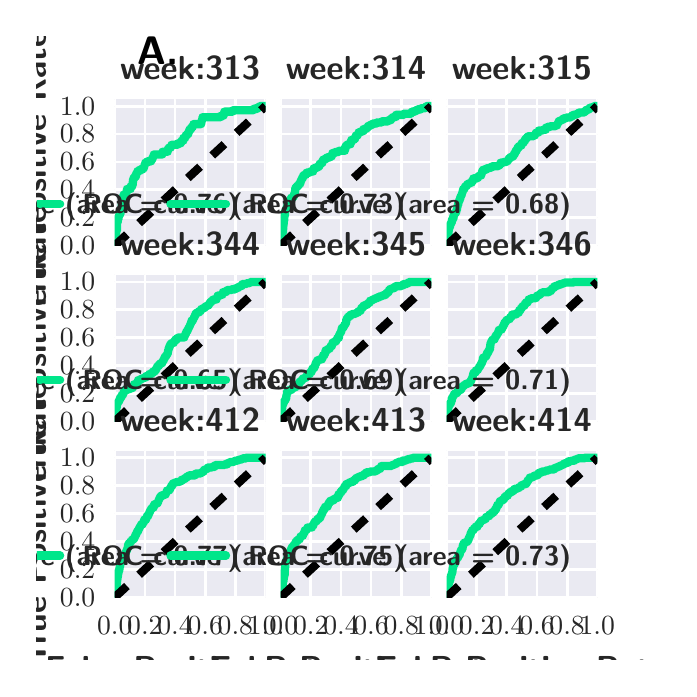
\begin{tikzpicture}[font=\bf\sffamily\fontsize{8}{8}\selectfont]
      \def\XST{-0.25in}
      \def\YST{0.25in}
      \node[] (A) {%% Creator: Matplotlib, PGF backend
%%
%% To include the figure in your LaTeX document, write
%%   \input{<filename>.pgf}
%%
%% Make sure the required packages are loaded in your preamble
%%   \usepackage{pgf}
%%
%% Figures using additional raster images can only be included by \input if
%% they are in the same directory as the main LaTeX file. For loading figures
%% from other directories you can use the `import` package
%%   \usepackage{import}
%% and then include the figures with
%%   \import{<path to file>}{<filename>.pgf}
%%
%% Matplotlib used the following preamble
%%   \usepackage[utf8x]{inputenc}
%%   \usepackage[T1]{fontenc}
%%
\begingroup%
\makeatletter%
\begin{pgfpicture}%
\pgfpathrectangle{\pgfpointorigin}{\pgfqpoint{3.113325in}{3.113325in}}%
\pgfusepath{use as bounding box, clip}%
\begin{pgfscope}%
\pgfsetbuttcap%
\pgfsetmiterjoin%
\definecolor{currentfill}{rgb}{1.000000,1.000000,1.000000}%
\pgfsetfillcolor{currentfill}%
\pgfsetlinewidth{0.000000pt}%
\definecolor{currentstroke}{rgb}{1.000000,1.000000,1.000000}%
\pgfsetstrokecolor{currentstroke}%
\pgfsetdash{}{0pt}%
\pgfpathmoveto{\pgfqpoint{0.000000in}{0.000000in}}%
\pgfpathlineto{\pgfqpoint{3.113325in}{0.000000in}}%
\pgfpathlineto{\pgfqpoint{3.113325in}{3.113325in}}%
\pgfpathlineto{\pgfqpoint{0.000000in}{3.113325in}}%
\pgfpathclose%
\pgfusepath{fill}%
\end{pgfscope}%
\begin{pgfscope}%
\pgfsetbuttcap%
\pgfsetmiterjoin%
\definecolor{currentfill}{rgb}{0.917647,0.917647,0.949020}%
\pgfsetfillcolor{currentfill}%
\pgfsetlinewidth{0.000000pt}%
\definecolor{currentstroke}{rgb}{0.000000,0.000000,0.000000}%
\pgfsetstrokecolor{currentstroke}%
\pgfsetstrokeopacity{0.000000}%
\pgfsetdash{}{0pt}%
\pgfpathmoveto{\pgfqpoint{0.389166in}{2.069445in}}%
\pgfpathlineto{\pgfqpoint{1.143174in}{2.069445in}}%
\pgfpathlineto{\pgfqpoint{1.143174in}{2.801993in}}%
\pgfpathlineto{\pgfqpoint{0.389166in}{2.801993in}}%
\pgfpathclose%
\pgfusepath{fill}%
\end{pgfscope}%
\begin{pgfscope}%
\pgfpathrectangle{\pgfqpoint{0.389166in}{2.069445in}}{\pgfqpoint{0.754008in}{0.732547in}} %
\pgfusepath{clip}%
\pgfsetroundcap%
\pgfsetroundjoin%
\pgfsetlinewidth{1.003750pt}%
\definecolor{currentstroke}{rgb}{1.000000,1.000000,1.000000}%
\pgfsetstrokecolor{currentstroke}%
\pgfsetdash{}{0pt}%
\pgfpathmoveto{\pgfqpoint{0.389166in}{2.069445in}}%
\pgfpathlineto{\pgfqpoint{0.389166in}{2.801993in}}%
\pgfusepath{stroke}%
\end{pgfscope}%
\begin{pgfscope}%
\pgfsetbuttcap%
\pgfsetroundjoin%
\definecolor{currentfill}{rgb}{0.150000,0.150000,0.150000}%
\pgfsetfillcolor{currentfill}%
\pgfsetlinewidth{1.003750pt}%
\definecolor{currentstroke}{rgb}{0.150000,0.150000,0.150000}%
\pgfsetstrokecolor{currentstroke}%
\pgfsetdash{}{0pt}%
\pgfsys@defobject{currentmarker}{\pgfqpoint{0.000000in}{0.000000in}}{\pgfqpoint{0.000000in}{0.000000in}}{%
\pgfpathmoveto{\pgfqpoint{0.000000in}{0.000000in}}%
\pgfpathlineto{\pgfqpoint{0.000000in}{0.000000in}}%
\pgfusepath{stroke,fill}%
}%
\begin{pgfscope}%
\pgfsys@transformshift{0.389166in}{2.069445in}%
\pgfsys@useobject{currentmarker}{}%
\end{pgfscope}%
\end{pgfscope}%
\begin{pgfscope}%
\pgfsetbuttcap%
\pgfsetroundjoin%
\definecolor{currentfill}{rgb}{0.150000,0.150000,0.150000}%
\pgfsetfillcolor{currentfill}%
\pgfsetlinewidth{1.003750pt}%
\definecolor{currentstroke}{rgb}{0.150000,0.150000,0.150000}%
\pgfsetstrokecolor{currentstroke}%
\pgfsetdash{}{0pt}%
\pgfsys@defobject{currentmarker}{\pgfqpoint{0.000000in}{0.000000in}}{\pgfqpoint{0.000000in}{0.000000in}}{%
\pgfpathmoveto{\pgfqpoint{0.000000in}{0.000000in}}%
\pgfpathlineto{\pgfqpoint{0.000000in}{0.000000in}}%
\pgfusepath{stroke,fill}%
}%
\begin{pgfscope}%
\pgfsys@transformshift{0.389166in}{2.801993in}%
\pgfsys@useobject{currentmarker}{}%
\end{pgfscope}%
\end{pgfscope}%
\begin{pgfscope}%
\pgfpathrectangle{\pgfqpoint{0.389166in}{2.069445in}}{\pgfqpoint{0.754008in}{0.732547in}} %
\pgfusepath{clip}%
\pgfsetroundcap%
\pgfsetroundjoin%
\pgfsetlinewidth{1.003750pt}%
\definecolor{currentstroke}{rgb}{1.000000,1.000000,1.000000}%
\pgfsetstrokecolor{currentstroke}%
\pgfsetdash{}{0pt}%
\pgfpathmoveto{\pgfqpoint{0.539967in}{2.069445in}}%
\pgfpathlineto{\pgfqpoint{0.539967in}{2.801993in}}%
\pgfusepath{stroke}%
\end{pgfscope}%
\begin{pgfscope}%
\pgfsetbuttcap%
\pgfsetroundjoin%
\definecolor{currentfill}{rgb}{0.150000,0.150000,0.150000}%
\pgfsetfillcolor{currentfill}%
\pgfsetlinewidth{1.003750pt}%
\definecolor{currentstroke}{rgb}{0.150000,0.150000,0.150000}%
\pgfsetstrokecolor{currentstroke}%
\pgfsetdash{}{0pt}%
\pgfsys@defobject{currentmarker}{\pgfqpoint{0.000000in}{0.000000in}}{\pgfqpoint{0.000000in}{0.000000in}}{%
\pgfpathmoveto{\pgfqpoint{0.000000in}{0.000000in}}%
\pgfpathlineto{\pgfqpoint{0.000000in}{0.000000in}}%
\pgfusepath{stroke,fill}%
}%
\begin{pgfscope}%
\pgfsys@transformshift{0.539967in}{2.069445in}%
\pgfsys@useobject{currentmarker}{}%
\end{pgfscope}%
\end{pgfscope}%
\begin{pgfscope}%
\pgfsetbuttcap%
\pgfsetroundjoin%
\definecolor{currentfill}{rgb}{0.150000,0.150000,0.150000}%
\pgfsetfillcolor{currentfill}%
\pgfsetlinewidth{1.003750pt}%
\definecolor{currentstroke}{rgb}{0.150000,0.150000,0.150000}%
\pgfsetstrokecolor{currentstroke}%
\pgfsetdash{}{0pt}%
\pgfsys@defobject{currentmarker}{\pgfqpoint{0.000000in}{0.000000in}}{\pgfqpoint{0.000000in}{0.000000in}}{%
\pgfpathmoveto{\pgfqpoint{0.000000in}{0.000000in}}%
\pgfpathlineto{\pgfqpoint{0.000000in}{0.000000in}}%
\pgfusepath{stroke,fill}%
}%
\begin{pgfscope}%
\pgfsys@transformshift{0.539967in}{2.801993in}%
\pgfsys@useobject{currentmarker}{}%
\end{pgfscope}%
\end{pgfscope}%
\begin{pgfscope}%
\pgfpathrectangle{\pgfqpoint{0.389166in}{2.069445in}}{\pgfqpoint{0.754008in}{0.732547in}} %
\pgfusepath{clip}%
\pgfsetroundcap%
\pgfsetroundjoin%
\pgfsetlinewidth{1.003750pt}%
\definecolor{currentstroke}{rgb}{1.000000,1.000000,1.000000}%
\pgfsetstrokecolor{currentstroke}%
\pgfsetdash{}{0pt}%
\pgfpathmoveto{\pgfqpoint{0.690769in}{2.069445in}}%
\pgfpathlineto{\pgfqpoint{0.690769in}{2.801993in}}%
\pgfusepath{stroke}%
\end{pgfscope}%
\begin{pgfscope}%
\pgfsetbuttcap%
\pgfsetroundjoin%
\definecolor{currentfill}{rgb}{0.150000,0.150000,0.150000}%
\pgfsetfillcolor{currentfill}%
\pgfsetlinewidth{1.003750pt}%
\definecolor{currentstroke}{rgb}{0.150000,0.150000,0.150000}%
\pgfsetstrokecolor{currentstroke}%
\pgfsetdash{}{0pt}%
\pgfsys@defobject{currentmarker}{\pgfqpoint{0.000000in}{0.000000in}}{\pgfqpoint{0.000000in}{0.000000in}}{%
\pgfpathmoveto{\pgfqpoint{0.000000in}{0.000000in}}%
\pgfpathlineto{\pgfqpoint{0.000000in}{0.000000in}}%
\pgfusepath{stroke,fill}%
}%
\begin{pgfscope}%
\pgfsys@transformshift{0.690769in}{2.069445in}%
\pgfsys@useobject{currentmarker}{}%
\end{pgfscope}%
\end{pgfscope}%
\begin{pgfscope}%
\pgfsetbuttcap%
\pgfsetroundjoin%
\definecolor{currentfill}{rgb}{0.150000,0.150000,0.150000}%
\pgfsetfillcolor{currentfill}%
\pgfsetlinewidth{1.003750pt}%
\definecolor{currentstroke}{rgb}{0.150000,0.150000,0.150000}%
\pgfsetstrokecolor{currentstroke}%
\pgfsetdash{}{0pt}%
\pgfsys@defobject{currentmarker}{\pgfqpoint{0.000000in}{0.000000in}}{\pgfqpoint{0.000000in}{0.000000in}}{%
\pgfpathmoveto{\pgfqpoint{0.000000in}{0.000000in}}%
\pgfpathlineto{\pgfqpoint{0.000000in}{0.000000in}}%
\pgfusepath{stroke,fill}%
}%
\begin{pgfscope}%
\pgfsys@transformshift{0.690769in}{2.801993in}%
\pgfsys@useobject{currentmarker}{}%
\end{pgfscope}%
\end{pgfscope}%
\begin{pgfscope}%
\pgfpathrectangle{\pgfqpoint{0.389166in}{2.069445in}}{\pgfqpoint{0.754008in}{0.732547in}} %
\pgfusepath{clip}%
\pgfsetroundcap%
\pgfsetroundjoin%
\pgfsetlinewidth{1.003750pt}%
\definecolor{currentstroke}{rgb}{1.000000,1.000000,1.000000}%
\pgfsetstrokecolor{currentstroke}%
\pgfsetdash{}{0pt}%
\pgfpathmoveto{\pgfqpoint{0.841571in}{2.069445in}}%
\pgfpathlineto{\pgfqpoint{0.841571in}{2.801993in}}%
\pgfusepath{stroke}%
\end{pgfscope}%
\begin{pgfscope}%
\pgfsetbuttcap%
\pgfsetroundjoin%
\definecolor{currentfill}{rgb}{0.150000,0.150000,0.150000}%
\pgfsetfillcolor{currentfill}%
\pgfsetlinewidth{1.003750pt}%
\definecolor{currentstroke}{rgb}{0.150000,0.150000,0.150000}%
\pgfsetstrokecolor{currentstroke}%
\pgfsetdash{}{0pt}%
\pgfsys@defobject{currentmarker}{\pgfqpoint{0.000000in}{0.000000in}}{\pgfqpoint{0.000000in}{0.000000in}}{%
\pgfpathmoveto{\pgfqpoint{0.000000in}{0.000000in}}%
\pgfpathlineto{\pgfqpoint{0.000000in}{0.000000in}}%
\pgfusepath{stroke,fill}%
}%
\begin{pgfscope}%
\pgfsys@transformshift{0.841571in}{2.069445in}%
\pgfsys@useobject{currentmarker}{}%
\end{pgfscope}%
\end{pgfscope}%
\begin{pgfscope}%
\pgfsetbuttcap%
\pgfsetroundjoin%
\definecolor{currentfill}{rgb}{0.150000,0.150000,0.150000}%
\pgfsetfillcolor{currentfill}%
\pgfsetlinewidth{1.003750pt}%
\definecolor{currentstroke}{rgb}{0.150000,0.150000,0.150000}%
\pgfsetstrokecolor{currentstroke}%
\pgfsetdash{}{0pt}%
\pgfsys@defobject{currentmarker}{\pgfqpoint{0.000000in}{0.000000in}}{\pgfqpoint{0.000000in}{0.000000in}}{%
\pgfpathmoveto{\pgfqpoint{0.000000in}{0.000000in}}%
\pgfpathlineto{\pgfqpoint{0.000000in}{0.000000in}}%
\pgfusepath{stroke,fill}%
}%
\begin{pgfscope}%
\pgfsys@transformshift{0.841571in}{2.801993in}%
\pgfsys@useobject{currentmarker}{}%
\end{pgfscope}%
\end{pgfscope}%
\begin{pgfscope}%
\pgfpathrectangle{\pgfqpoint{0.389166in}{2.069445in}}{\pgfqpoint{0.754008in}{0.732547in}} %
\pgfusepath{clip}%
\pgfsetroundcap%
\pgfsetroundjoin%
\pgfsetlinewidth{1.003750pt}%
\definecolor{currentstroke}{rgb}{1.000000,1.000000,1.000000}%
\pgfsetstrokecolor{currentstroke}%
\pgfsetdash{}{0pt}%
\pgfpathmoveto{\pgfqpoint{0.992372in}{2.069445in}}%
\pgfpathlineto{\pgfqpoint{0.992372in}{2.801993in}}%
\pgfusepath{stroke}%
\end{pgfscope}%
\begin{pgfscope}%
\pgfsetbuttcap%
\pgfsetroundjoin%
\definecolor{currentfill}{rgb}{0.150000,0.150000,0.150000}%
\pgfsetfillcolor{currentfill}%
\pgfsetlinewidth{1.003750pt}%
\definecolor{currentstroke}{rgb}{0.150000,0.150000,0.150000}%
\pgfsetstrokecolor{currentstroke}%
\pgfsetdash{}{0pt}%
\pgfsys@defobject{currentmarker}{\pgfqpoint{0.000000in}{0.000000in}}{\pgfqpoint{0.000000in}{0.000000in}}{%
\pgfpathmoveto{\pgfqpoint{0.000000in}{0.000000in}}%
\pgfpathlineto{\pgfqpoint{0.000000in}{0.000000in}}%
\pgfusepath{stroke,fill}%
}%
\begin{pgfscope}%
\pgfsys@transformshift{0.992372in}{2.069445in}%
\pgfsys@useobject{currentmarker}{}%
\end{pgfscope}%
\end{pgfscope}%
\begin{pgfscope}%
\pgfsetbuttcap%
\pgfsetroundjoin%
\definecolor{currentfill}{rgb}{0.150000,0.150000,0.150000}%
\pgfsetfillcolor{currentfill}%
\pgfsetlinewidth{1.003750pt}%
\definecolor{currentstroke}{rgb}{0.150000,0.150000,0.150000}%
\pgfsetstrokecolor{currentstroke}%
\pgfsetdash{}{0pt}%
\pgfsys@defobject{currentmarker}{\pgfqpoint{0.000000in}{0.000000in}}{\pgfqpoint{0.000000in}{0.000000in}}{%
\pgfpathmoveto{\pgfqpoint{0.000000in}{0.000000in}}%
\pgfpathlineto{\pgfqpoint{0.000000in}{0.000000in}}%
\pgfusepath{stroke,fill}%
}%
\begin{pgfscope}%
\pgfsys@transformshift{0.992372in}{2.801993in}%
\pgfsys@useobject{currentmarker}{}%
\end{pgfscope}%
\end{pgfscope}%
\begin{pgfscope}%
\pgfpathrectangle{\pgfqpoint{0.389166in}{2.069445in}}{\pgfqpoint{0.754008in}{0.732547in}} %
\pgfusepath{clip}%
\pgfsetroundcap%
\pgfsetroundjoin%
\pgfsetlinewidth{1.003750pt}%
\definecolor{currentstroke}{rgb}{1.000000,1.000000,1.000000}%
\pgfsetstrokecolor{currentstroke}%
\pgfsetdash{}{0pt}%
\pgfpathmoveto{\pgfqpoint{1.143174in}{2.069445in}}%
\pgfpathlineto{\pgfqpoint{1.143174in}{2.801993in}}%
\pgfusepath{stroke}%
\end{pgfscope}%
\begin{pgfscope}%
\pgfsetbuttcap%
\pgfsetroundjoin%
\definecolor{currentfill}{rgb}{0.150000,0.150000,0.150000}%
\pgfsetfillcolor{currentfill}%
\pgfsetlinewidth{1.003750pt}%
\definecolor{currentstroke}{rgb}{0.150000,0.150000,0.150000}%
\pgfsetstrokecolor{currentstroke}%
\pgfsetdash{}{0pt}%
\pgfsys@defobject{currentmarker}{\pgfqpoint{0.000000in}{0.000000in}}{\pgfqpoint{0.000000in}{0.000000in}}{%
\pgfpathmoveto{\pgfqpoint{0.000000in}{0.000000in}}%
\pgfpathlineto{\pgfqpoint{0.000000in}{0.000000in}}%
\pgfusepath{stroke,fill}%
}%
\begin{pgfscope}%
\pgfsys@transformshift{1.143174in}{2.069445in}%
\pgfsys@useobject{currentmarker}{}%
\end{pgfscope}%
\end{pgfscope}%
\begin{pgfscope}%
\pgfsetbuttcap%
\pgfsetroundjoin%
\definecolor{currentfill}{rgb}{0.150000,0.150000,0.150000}%
\pgfsetfillcolor{currentfill}%
\pgfsetlinewidth{1.003750pt}%
\definecolor{currentstroke}{rgb}{0.150000,0.150000,0.150000}%
\pgfsetstrokecolor{currentstroke}%
\pgfsetdash{}{0pt}%
\pgfsys@defobject{currentmarker}{\pgfqpoint{0.000000in}{0.000000in}}{\pgfqpoint{0.000000in}{0.000000in}}{%
\pgfpathmoveto{\pgfqpoint{0.000000in}{0.000000in}}%
\pgfpathlineto{\pgfqpoint{0.000000in}{0.000000in}}%
\pgfusepath{stroke,fill}%
}%
\begin{pgfscope}%
\pgfsys@transformshift{1.143174in}{2.801993in}%
\pgfsys@useobject{currentmarker}{}%
\end{pgfscope}%
\end{pgfscope}%
\begin{pgfscope}%
\pgfpathrectangle{\pgfqpoint{0.389166in}{2.069445in}}{\pgfqpoint{0.754008in}{0.732547in}} %
\pgfusepath{clip}%
\pgfsetroundcap%
\pgfsetroundjoin%
\pgfsetlinewidth{1.003750pt}%
\definecolor{currentstroke}{rgb}{1.000000,1.000000,1.000000}%
\pgfsetstrokecolor{currentstroke}%
\pgfsetdash{}{0pt}%
\pgfpathmoveto{\pgfqpoint{0.389166in}{2.069445in}}%
\pgfpathlineto{\pgfqpoint{1.143174in}{2.069445in}}%
\pgfusepath{stroke}%
\end{pgfscope}%
\begin{pgfscope}%
\pgfsetbuttcap%
\pgfsetroundjoin%
\definecolor{currentfill}{rgb}{0.150000,0.150000,0.150000}%
\pgfsetfillcolor{currentfill}%
\pgfsetlinewidth{1.003750pt}%
\definecolor{currentstroke}{rgb}{0.150000,0.150000,0.150000}%
\pgfsetstrokecolor{currentstroke}%
\pgfsetdash{}{0pt}%
\pgfsys@defobject{currentmarker}{\pgfqpoint{0.000000in}{0.000000in}}{\pgfqpoint{0.000000in}{0.000000in}}{%
\pgfpathmoveto{\pgfqpoint{0.000000in}{0.000000in}}%
\pgfpathlineto{\pgfqpoint{0.000000in}{0.000000in}}%
\pgfusepath{stroke,fill}%
}%
\begin{pgfscope}%
\pgfsys@transformshift{0.389166in}{2.069445in}%
\pgfsys@useobject{currentmarker}{}%
\end{pgfscope}%
\end{pgfscope}%
\begin{pgfscope}%
\pgfsetbuttcap%
\pgfsetroundjoin%
\definecolor{currentfill}{rgb}{0.150000,0.150000,0.150000}%
\pgfsetfillcolor{currentfill}%
\pgfsetlinewidth{1.003750pt}%
\definecolor{currentstroke}{rgb}{0.150000,0.150000,0.150000}%
\pgfsetstrokecolor{currentstroke}%
\pgfsetdash{}{0pt}%
\pgfsys@defobject{currentmarker}{\pgfqpoint{0.000000in}{0.000000in}}{\pgfqpoint{0.000000in}{0.000000in}}{%
\pgfpathmoveto{\pgfqpoint{0.000000in}{0.000000in}}%
\pgfpathlineto{\pgfqpoint{0.000000in}{0.000000in}}%
\pgfusepath{stroke,fill}%
}%
\begin{pgfscope}%
\pgfsys@transformshift{1.143174in}{2.069445in}%
\pgfsys@useobject{currentmarker}{}%
\end{pgfscope}%
\end{pgfscope}%
\begin{pgfscope}%
\definecolor{textcolor}{rgb}{0.150000,0.150000,0.150000}%
\pgfsetstrokecolor{textcolor}%
\pgfsetfillcolor{textcolor}%
\pgftext[x=0.291943in,y=2.069445in,right,]{\color{textcolor}\sffamily\fontsize{10.000000}{12.000000}\bfseries\selectfont \(\displaystyle 0.0\)}%
\end{pgfscope}%
\begin{pgfscope}%
\pgfpathrectangle{\pgfqpoint{0.389166in}{2.069445in}}{\pgfqpoint{0.754008in}{0.732547in}} %
\pgfusepath{clip}%
\pgfsetroundcap%
\pgfsetroundjoin%
\pgfsetlinewidth{1.003750pt}%
\definecolor{currentstroke}{rgb}{1.000000,1.000000,1.000000}%
\pgfsetstrokecolor{currentstroke}%
\pgfsetdash{}{0pt}%
\pgfpathmoveto{\pgfqpoint{0.389166in}{2.208978in}}%
\pgfpathlineto{\pgfqpoint{1.143174in}{2.208978in}}%
\pgfusepath{stroke}%
\end{pgfscope}%
\begin{pgfscope}%
\pgfsetbuttcap%
\pgfsetroundjoin%
\definecolor{currentfill}{rgb}{0.150000,0.150000,0.150000}%
\pgfsetfillcolor{currentfill}%
\pgfsetlinewidth{1.003750pt}%
\definecolor{currentstroke}{rgb}{0.150000,0.150000,0.150000}%
\pgfsetstrokecolor{currentstroke}%
\pgfsetdash{}{0pt}%
\pgfsys@defobject{currentmarker}{\pgfqpoint{0.000000in}{0.000000in}}{\pgfqpoint{0.000000in}{0.000000in}}{%
\pgfpathmoveto{\pgfqpoint{0.000000in}{0.000000in}}%
\pgfpathlineto{\pgfqpoint{0.000000in}{0.000000in}}%
\pgfusepath{stroke,fill}%
}%
\begin{pgfscope}%
\pgfsys@transformshift{0.389166in}{2.208978in}%
\pgfsys@useobject{currentmarker}{}%
\end{pgfscope}%
\end{pgfscope}%
\begin{pgfscope}%
\pgfsetbuttcap%
\pgfsetroundjoin%
\definecolor{currentfill}{rgb}{0.150000,0.150000,0.150000}%
\pgfsetfillcolor{currentfill}%
\pgfsetlinewidth{1.003750pt}%
\definecolor{currentstroke}{rgb}{0.150000,0.150000,0.150000}%
\pgfsetstrokecolor{currentstroke}%
\pgfsetdash{}{0pt}%
\pgfsys@defobject{currentmarker}{\pgfqpoint{0.000000in}{0.000000in}}{\pgfqpoint{0.000000in}{0.000000in}}{%
\pgfpathmoveto{\pgfqpoint{0.000000in}{0.000000in}}%
\pgfpathlineto{\pgfqpoint{0.000000in}{0.000000in}}%
\pgfusepath{stroke,fill}%
}%
\begin{pgfscope}%
\pgfsys@transformshift{1.143174in}{2.208978in}%
\pgfsys@useobject{currentmarker}{}%
\end{pgfscope}%
\end{pgfscope}%
\begin{pgfscope}%
\definecolor{textcolor}{rgb}{0.150000,0.150000,0.150000}%
\pgfsetstrokecolor{textcolor}%
\pgfsetfillcolor{textcolor}%
\pgftext[x=0.291943in,y=2.208978in,right,]{\color{textcolor}\sffamily\fontsize{10.000000}{12.000000}\bfseries\selectfont \(\displaystyle 0.2\)}%
\end{pgfscope}%
\begin{pgfscope}%
\pgfpathrectangle{\pgfqpoint{0.389166in}{2.069445in}}{\pgfqpoint{0.754008in}{0.732547in}} %
\pgfusepath{clip}%
\pgfsetroundcap%
\pgfsetroundjoin%
\pgfsetlinewidth{1.003750pt}%
\definecolor{currentstroke}{rgb}{1.000000,1.000000,1.000000}%
\pgfsetstrokecolor{currentstroke}%
\pgfsetdash{}{0pt}%
\pgfpathmoveto{\pgfqpoint{0.389166in}{2.348511in}}%
\pgfpathlineto{\pgfqpoint{1.143174in}{2.348511in}}%
\pgfusepath{stroke}%
\end{pgfscope}%
\begin{pgfscope}%
\pgfsetbuttcap%
\pgfsetroundjoin%
\definecolor{currentfill}{rgb}{0.150000,0.150000,0.150000}%
\pgfsetfillcolor{currentfill}%
\pgfsetlinewidth{1.003750pt}%
\definecolor{currentstroke}{rgb}{0.150000,0.150000,0.150000}%
\pgfsetstrokecolor{currentstroke}%
\pgfsetdash{}{0pt}%
\pgfsys@defobject{currentmarker}{\pgfqpoint{0.000000in}{0.000000in}}{\pgfqpoint{0.000000in}{0.000000in}}{%
\pgfpathmoveto{\pgfqpoint{0.000000in}{0.000000in}}%
\pgfpathlineto{\pgfqpoint{0.000000in}{0.000000in}}%
\pgfusepath{stroke,fill}%
}%
\begin{pgfscope}%
\pgfsys@transformshift{0.389166in}{2.348511in}%
\pgfsys@useobject{currentmarker}{}%
\end{pgfscope}%
\end{pgfscope}%
\begin{pgfscope}%
\pgfsetbuttcap%
\pgfsetroundjoin%
\definecolor{currentfill}{rgb}{0.150000,0.150000,0.150000}%
\pgfsetfillcolor{currentfill}%
\pgfsetlinewidth{1.003750pt}%
\definecolor{currentstroke}{rgb}{0.150000,0.150000,0.150000}%
\pgfsetstrokecolor{currentstroke}%
\pgfsetdash{}{0pt}%
\pgfsys@defobject{currentmarker}{\pgfqpoint{0.000000in}{0.000000in}}{\pgfqpoint{0.000000in}{0.000000in}}{%
\pgfpathmoveto{\pgfqpoint{0.000000in}{0.000000in}}%
\pgfpathlineto{\pgfqpoint{0.000000in}{0.000000in}}%
\pgfusepath{stroke,fill}%
}%
\begin{pgfscope}%
\pgfsys@transformshift{1.143174in}{2.348511in}%
\pgfsys@useobject{currentmarker}{}%
\end{pgfscope}%
\end{pgfscope}%
\begin{pgfscope}%
\definecolor{textcolor}{rgb}{0.150000,0.150000,0.150000}%
\pgfsetstrokecolor{textcolor}%
\pgfsetfillcolor{textcolor}%
\pgftext[x=0.291943in,y=2.348511in,right,]{\color{textcolor}\sffamily\fontsize{10.000000}{12.000000}\bfseries\selectfont \(\displaystyle 0.4\)}%
\end{pgfscope}%
\begin{pgfscope}%
\pgfpathrectangle{\pgfqpoint{0.389166in}{2.069445in}}{\pgfqpoint{0.754008in}{0.732547in}} %
\pgfusepath{clip}%
\pgfsetroundcap%
\pgfsetroundjoin%
\pgfsetlinewidth{1.003750pt}%
\definecolor{currentstroke}{rgb}{1.000000,1.000000,1.000000}%
\pgfsetstrokecolor{currentstroke}%
\pgfsetdash{}{0pt}%
\pgfpathmoveto{\pgfqpoint{0.389166in}{2.488044in}}%
\pgfpathlineto{\pgfqpoint{1.143174in}{2.488044in}}%
\pgfusepath{stroke}%
\end{pgfscope}%
\begin{pgfscope}%
\pgfsetbuttcap%
\pgfsetroundjoin%
\definecolor{currentfill}{rgb}{0.150000,0.150000,0.150000}%
\pgfsetfillcolor{currentfill}%
\pgfsetlinewidth{1.003750pt}%
\definecolor{currentstroke}{rgb}{0.150000,0.150000,0.150000}%
\pgfsetstrokecolor{currentstroke}%
\pgfsetdash{}{0pt}%
\pgfsys@defobject{currentmarker}{\pgfqpoint{0.000000in}{0.000000in}}{\pgfqpoint{0.000000in}{0.000000in}}{%
\pgfpathmoveto{\pgfqpoint{0.000000in}{0.000000in}}%
\pgfpathlineto{\pgfqpoint{0.000000in}{0.000000in}}%
\pgfusepath{stroke,fill}%
}%
\begin{pgfscope}%
\pgfsys@transformshift{0.389166in}{2.488044in}%
\pgfsys@useobject{currentmarker}{}%
\end{pgfscope}%
\end{pgfscope}%
\begin{pgfscope}%
\pgfsetbuttcap%
\pgfsetroundjoin%
\definecolor{currentfill}{rgb}{0.150000,0.150000,0.150000}%
\pgfsetfillcolor{currentfill}%
\pgfsetlinewidth{1.003750pt}%
\definecolor{currentstroke}{rgb}{0.150000,0.150000,0.150000}%
\pgfsetstrokecolor{currentstroke}%
\pgfsetdash{}{0pt}%
\pgfsys@defobject{currentmarker}{\pgfqpoint{0.000000in}{0.000000in}}{\pgfqpoint{0.000000in}{0.000000in}}{%
\pgfpathmoveto{\pgfqpoint{0.000000in}{0.000000in}}%
\pgfpathlineto{\pgfqpoint{0.000000in}{0.000000in}}%
\pgfusepath{stroke,fill}%
}%
\begin{pgfscope}%
\pgfsys@transformshift{1.143174in}{2.488044in}%
\pgfsys@useobject{currentmarker}{}%
\end{pgfscope}%
\end{pgfscope}%
\begin{pgfscope}%
\definecolor{textcolor}{rgb}{0.150000,0.150000,0.150000}%
\pgfsetstrokecolor{textcolor}%
\pgfsetfillcolor{textcolor}%
\pgftext[x=0.291943in,y=2.488044in,right,]{\color{textcolor}\sffamily\fontsize{10.000000}{12.000000}\bfseries\selectfont \(\displaystyle 0.6\)}%
\end{pgfscope}%
\begin{pgfscope}%
\pgfpathrectangle{\pgfqpoint{0.389166in}{2.069445in}}{\pgfqpoint{0.754008in}{0.732547in}} %
\pgfusepath{clip}%
\pgfsetroundcap%
\pgfsetroundjoin%
\pgfsetlinewidth{1.003750pt}%
\definecolor{currentstroke}{rgb}{1.000000,1.000000,1.000000}%
\pgfsetstrokecolor{currentstroke}%
\pgfsetdash{}{0pt}%
\pgfpathmoveto{\pgfqpoint{0.389166in}{2.627577in}}%
\pgfpathlineto{\pgfqpoint{1.143174in}{2.627577in}}%
\pgfusepath{stroke}%
\end{pgfscope}%
\begin{pgfscope}%
\pgfsetbuttcap%
\pgfsetroundjoin%
\definecolor{currentfill}{rgb}{0.150000,0.150000,0.150000}%
\pgfsetfillcolor{currentfill}%
\pgfsetlinewidth{1.003750pt}%
\definecolor{currentstroke}{rgb}{0.150000,0.150000,0.150000}%
\pgfsetstrokecolor{currentstroke}%
\pgfsetdash{}{0pt}%
\pgfsys@defobject{currentmarker}{\pgfqpoint{0.000000in}{0.000000in}}{\pgfqpoint{0.000000in}{0.000000in}}{%
\pgfpathmoveto{\pgfqpoint{0.000000in}{0.000000in}}%
\pgfpathlineto{\pgfqpoint{0.000000in}{0.000000in}}%
\pgfusepath{stroke,fill}%
}%
\begin{pgfscope}%
\pgfsys@transformshift{0.389166in}{2.627577in}%
\pgfsys@useobject{currentmarker}{}%
\end{pgfscope}%
\end{pgfscope}%
\begin{pgfscope}%
\pgfsetbuttcap%
\pgfsetroundjoin%
\definecolor{currentfill}{rgb}{0.150000,0.150000,0.150000}%
\pgfsetfillcolor{currentfill}%
\pgfsetlinewidth{1.003750pt}%
\definecolor{currentstroke}{rgb}{0.150000,0.150000,0.150000}%
\pgfsetstrokecolor{currentstroke}%
\pgfsetdash{}{0pt}%
\pgfsys@defobject{currentmarker}{\pgfqpoint{0.000000in}{0.000000in}}{\pgfqpoint{0.000000in}{0.000000in}}{%
\pgfpathmoveto{\pgfqpoint{0.000000in}{0.000000in}}%
\pgfpathlineto{\pgfqpoint{0.000000in}{0.000000in}}%
\pgfusepath{stroke,fill}%
}%
\begin{pgfscope}%
\pgfsys@transformshift{1.143174in}{2.627577in}%
\pgfsys@useobject{currentmarker}{}%
\end{pgfscope}%
\end{pgfscope}%
\begin{pgfscope}%
\definecolor{textcolor}{rgb}{0.150000,0.150000,0.150000}%
\pgfsetstrokecolor{textcolor}%
\pgfsetfillcolor{textcolor}%
\pgftext[x=0.291943in,y=2.627577in,right,]{\color{textcolor}\sffamily\fontsize{10.000000}{12.000000}\bfseries\selectfont \(\displaystyle 0.8\)}%
\end{pgfscope}%
\begin{pgfscope}%
\pgfpathrectangle{\pgfqpoint{0.389166in}{2.069445in}}{\pgfqpoint{0.754008in}{0.732547in}} %
\pgfusepath{clip}%
\pgfsetroundcap%
\pgfsetroundjoin%
\pgfsetlinewidth{1.003750pt}%
\definecolor{currentstroke}{rgb}{1.000000,1.000000,1.000000}%
\pgfsetstrokecolor{currentstroke}%
\pgfsetdash{}{0pt}%
\pgfpathmoveto{\pgfqpoint{0.389166in}{2.767109in}}%
\pgfpathlineto{\pgfqpoint{1.143174in}{2.767109in}}%
\pgfusepath{stroke}%
\end{pgfscope}%
\begin{pgfscope}%
\pgfsetbuttcap%
\pgfsetroundjoin%
\definecolor{currentfill}{rgb}{0.150000,0.150000,0.150000}%
\pgfsetfillcolor{currentfill}%
\pgfsetlinewidth{1.003750pt}%
\definecolor{currentstroke}{rgb}{0.150000,0.150000,0.150000}%
\pgfsetstrokecolor{currentstroke}%
\pgfsetdash{}{0pt}%
\pgfsys@defobject{currentmarker}{\pgfqpoint{0.000000in}{0.000000in}}{\pgfqpoint{0.000000in}{0.000000in}}{%
\pgfpathmoveto{\pgfqpoint{0.000000in}{0.000000in}}%
\pgfpathlineto{\pgfqpoint{0.000000in}{0.000000in}}%
\pgfusepath{stroke,fill}%
}%
\begin{pgfscope}%
\pgfsys@transformshift{0.389166in}{2.767109in}%
\pgfsys@useobject{currentmarker}{}%
\end{pgfscope}%
\end{pgfscope}%
\begin{pgfscope}%
\pgfsetbuttcap%
\pgfsetroundjoin%
\definecolor{currentfill}{rgb}{0.150000,0.150000,0.150000}%
\pgfsetfillcolor{currentfill}%
\pgfsetlinewidth{1.003750pt}%
\definecolor{currentstroke}{rgb}{0.150000,0.150000,0.150000}%
\pgfsetstrokecolor{currentstroke}%
\pgfsetdash{}{0pt}%
\pgfsys@defobject{currentmarker}{\pgfqpoint{0.000000in}{0.000000in}}{\pgfqpoint{0.000000in}{0.000000in}}{%
\pgfpathmoveto{\pgfqpoint{0.000000in}{0.000000in}}%
\pgfpathlineto{\pgfqpoint{0.000000in}{0.000000in}}%
\pgfusepath{stroke,fill}%
}%
\begin{pgfscope}%
\pgfsys@transformshift{1.143174in}{2.767109in}%
\pgfsys@useobject{currentmarker}{}%
\end{pgfscope}%
\end{pgfscope}%
\begin{pgfscope}%
\definecolor{textcolor}{rgb}{0.150000,0.150000,0.150000}%
\pgfsetstrokecolor{textcolor}%
\pgfsetfillcolor{textcolor}%
\pgftext[x=0.291943in,y=2.767109in,right,]{\color{textcolor}\sffamily\fontsize{10.000000}{12.000000}\bfseries\selectfont \(\displaystyle 1.0\)}%
\end{pgfscope}%
\begin{pgfscope}%
\definecolor{textcolor}{rgb}{0.150000,0.150000,0.150000}%
\pgfsetstrokecolor{textcolor}%
\pgfsetfillcolor{textcolor}%
\pgftext[x=0.045029in,y=2.435719in,,bottom,rotate=90.000000]{\color{textcolor}\sffamily\fontsize{12.000000}{14.400000}\bfseries\selectfont True Positive Rate}%
\end{pgfscope}%
\begin{pgfscope}%
\pgfpathrectangle{\pgfqpoint{0.389166in}{2.069445in}}{\pgfqpoint{0.754008in}{0.732547in}} %
\pgfusepath{clip}%
\pgfsetroundcap%
\pgfsetroundjoin%
\pgfsetlinewidth{3.011250pt}%
\definecolor{currentstroke}{rgb}{0.000000,0.901961,0.541176}%
\pgfsetstrokecolor{currentstroke}%
\pgfsetdash{}{0pt}%
\pgfpathmoveto{\pgfqpoint{0.389166in}{2.076353in}}%
\pgfpathlineto{\pgfqpoint{0.389421in}{2.076353in}}%
\pgfpathlineto{\pgfqpoint{0.389677in}{2.097076in}}%
\pgfpathlineto{\pgfqpoint{0.390955in}{2.097076in}}%
\pgfpathlineto{\pgfqpoint{0.391978in}{2.117798in}}%
\pgfpathlineto{\pgfqpoint{0.392745in}{2.117798in}}%
\pgfpathlineto{\pgfqpoint{0.392745in}{2.124706in}}%
\pgfpathlineto{\pgfqpoint{0.394791in}{2.124706in}}%
\pgfpathlineto{\pgfqpoint{0.394791in}{2.131614in}}%
\pgfpathlineto{\pgfqpoint{0.396325in}{2.131614in}}%
\pgfpathlineto{\pgfqpoint{0.396325in}{2.138521in}}%
\pgfpathlineto{\pgfqpoint{0.397603in}{2.138521in}}%
\pgfpathlineto{\pgfqpoint{0.397603in}{2.145429in}}%
\pgfpathlineto{\pgfqpoint{0.400160in}{2.145429in}}%
\pgfpathlineto{\pgfqpoint{0.400927in}{2.179966in}}%
\pgfpathlineto{\pgfqpoint{0.401694in}{2.179966in}}%
\pgfpathlineto{\pgfqpoint{0.401694in}{2.186874in}}%
\pgfpathlineto{\pgfqpoint{0.404251in}{2.186874in}}%
\pgfpathlineto{\pgfqpoint{0.404507in}{2.200689in}}%
\pgfpathlineto{\pgfqpoint{0.407319in}{2.200689in}}%
\pgfpathlineto{\pgfqpoint{0.407575in}{2.214504in}}%
\pgfpathlineto{\pgfqpoint{0.410643in}{2.214504in}}%
\pgfpathlineto{\pgfqpoint{0.410643in}{2.221412in}}%
\pgfpathlineto{\pgfqpoint{0.413967in}{2.221412in}}%
\pgfpathlineto{\pgfqpoint{0.413967in}{2.228319in}}%
\pgfpathlineto{\pgfqpoint{0.417802in}{2.228319in}}%
\pgfpathlineto{\pgfqpoint{0.418825in}{2.242135in}}%
\pgfpathlineto{\pgfqpoint{0.419336in}{2.242135in}}%
\pgfpathlineto{\pgfqpoint{0.419336in}{2.249042in}}%
\pgfpathlineto{\pgfqpoint{0.421893in}{2.249042in}}%
\pgfpathlineto{\pgfqpoint{0.421893in}{2.255950in}}%
\pgfpathlineto{\pgfqpoint{0.423938in}{2.255950in}}%
\pgfpathlineto{\pgfqpoint{0.424706in}{2.276672in}}%
\pgfpathlineto{\pgfqpoint{0.425217in}{2.276672in}}%
\pgfpathlineto{\pgfqpoint{0.426240in}{2.290487in}}%
\pgfpathlineto{\pgfqpoint{0.427262in}{2.290487in}}%
\pgfpathlineto{\pgfqpoint{0.427262in}{2.297395in}}%
\pgfpathlineto{\pgfqpoint{0.428796in}{2.297395in}}%
\pgfpathlineto{\pgfqpoint{0.428796in}{2.304303in}}%
\pgfpathlineto{\pgfqpoint{0.431098in}{2.304303in}}%
\pgfpathlineto{\pgfqpoint{0.431098in}{2.311210in}}%
\pgfpathlineto{\pgfqpoint{0.432376in}{2.311210in}}%
\pgfpathlineto{\pgfqpoint{0.432376in}{2.318118in}}%
\pgfpathlineto{\pgfqpoint{0.433399in}{2.318118in}}%
\pgfpathlineto{\pgfqpoint{0.433654in}{2.318118in}}%
\pgfpathlineto{\pgfqpoint{0.433654in}{2.325025in}}%
\pgfpathlineto{\pgfqpoint{0.444649in}{2.325025in}}%
\pgfpathlineto{\pgfqpoint{0.444649in}{2.331933in}}%
\pgfpathlineto{\pgfqpoint{0.447717in}{2.331933in}}%
\pgfpathlineto{\pgfqpoint{0.447717in}{2.338840in}}%
\pgfpathlineto{\pgfqpoint{0.449507in}{2.338840in}}%
\pgfpathlineto{\pgfqpoint{0.450274in}{2.352656in}}%
\pgfpathlineto{\pgfqpoint{0.468683in}{2.352656in}}%
\pgfpathlineto{\pgfqpoint{0.468939in}{2.366471in}}%
\pgfpathlineto{\pgfqpoint{0.477120in}{2.366471in}}%
\pgfpathlineto{\pgfqpoint{0.477120in}{2.373378in}}%
\pgfpathlineto{\pgfqpoint{0.477632in}{2.373378in}}%
\pgfpathlineto{\pgfqpoint{0.479166in}{2.373378in}}%
\pgfpathlineto{\pgfqpoint{0.480189in}{2.394101in}}%
\pgfpathlineto{\pgfqpoint{0.480444in}{2.394101in}}%
\pgfpathlineto{\pgfqpoint{0.480444in}{2.401008in}}%
\pgfpathlineto{\pgfqpoint{0.483001in}{2.401008in}}%
\pgfpathlineto{\pgfqpoint{0.483001in}{2.407916in}}%
\pgfpathlineto{\pgfqpoint{0.488626in}{2.407916in}}%
\pgfpathlineto{\pgfqpoint{0.488626in}{2.414824in}}%
\pgfpathlineto{\pgfqpoint{0.495530in}{2.414824in}}%
\pgfpathlineto{\pgfqpoint{0.495530in}{2.428639in}}%
\pgfpathlineto{\pgfqpoint{0.499621in}{2.428639in}}%
\pgfpathlineto{\pgfqpoint{0.499621in}{2.435546in}}%
\pgfpathlineto{\pgfqpoint{0.502944in}{2.435546in}}%
\pgfpathlineto{\pgfqpoint{0.502944in}{2.442454in}}%
\pgfpathlineto{\pgfqpoint{0.513683in}{2.442454in}}%
\pgfpathlineto{\pgfqpoint{0.513683in}{2.449361in}}%
\pgfpathlineto{\pgfqpoint{0.527234in}{2.449361in}}%
\pgfpathlineto{\pgfqpoint{0.527234in}{2.456269in}}%
\pgfpathlineto{\pgfqpoint{0.534905in}{2.456269in}}%
\pgfpathlineto{\pgfqpoint{0.534905in}{2.463177in}}%
\pgfpathlineto{\pgfqpoint{0.536950in}{2.463177in}}%
\pgfpathlineto{\pgfqpoint{0.536950in}{2.470084in}}%
\pgfpathlineto{\pgfqpoint{0.538996in}{2.470084in}}%
\pgfpathlineto{\pgfqpoint{0.538996in}{2.476992in}}%
\pgfpathlineto{\pgfqpoint{0.541553in}{2.476992in}}%
\pgfpathlineto{\pgfqpoint{0.541553in}{2.483899in}}%
\pgfpathlineto{\pgfqpoint{0.551013in}{2.483899in}}%
\pgfpathlineto{\pgfqpoint{0.551013in}{2.490807in}}%
\pgfpathlineto{\pgfqpoint{0.570956in}{2.490807in}}%
\pgfpathlineto{\pgfqpoint{0.571212in}{2.497714in}}%
\pgfpathlineto{\pgfqpoint{0.575047in}{2.497714in}}%
\pgfpathlineto{\pgfqpoint{0.575047in}{2.504622in}}%
\pgfpathlineto{\pgfqpoint{0.579394in}{2.504622in}}%
\pgfpathlineto{\pgfqpoint{0.579394in}{2.511529in}}%
\pgfpathlineto{\pgfqpoint{0.581695in}{2.511529in}}%
\pgfpathlineto{\pgfqpoint{0.581695in}{2.518437in}}%
\pgfpathlineto{\pgfqpoint{0.584252in}{2.518437in}}%
\pgfpathlineto{\pgfqpoint{0.584252in}{2.525345in}}%
\pgfpathlineto{\pgfqpoint{0.627206in}{2.525345in}}%
\pgfpathlineto{\pgfqpoint{0.627973in}{2.539160in}}%
\pgfpathlineto{\pgfqpoint{0.654053in}{2.539160in}}%
\pgfpathlineto{\pgfqpoint{0.654564in}{2.552975in}}%
\pgfpathlineto{\pgfqpoint{0.660189in}{2.552975in}}%
\pgfpathlineto{\pgfqpoint{0.660189in}{2.559882in}}%
\pgfpathlineto{\pgfqpoint{0.669650in}{2.559882in}}%
\pgfpathlineto{\pgfqpoint{0.669650in}{2.566790in}}%
\pgfpathlineto{\pgfqpoint{0.672973in}{2.566790in}}%
\pgfpathlineto{\pgfqpoint{0.672973in}{2.573698in}}%
\pgfpathlineto{\pgfqpoint{0.702888in}{2.573698in}}%
\pgfpathlineto{\pgfqpoint{0.702888in}{2.580605in}}%
\pgfpathlineto{\pgfqpoint{0.703911in}{2.580605in}}%
\pgfpathlineto{\pgfqpoint{0.718485in}{2.580605in}}%
\pgfpathlineto{\pgfqpoint{0.718485in}{2.587513in}}%
\pgfpathlineto{\pgfqpoint{0.723599in}{2.587513in}}%
\pgfpathlineto{\pgfqpoint{0.723599in}{2.594420in}}%
\pgfpathlineto{\pgfqpoint{0.732548in}{2.594420in}}%
\pgfpathlineto{\pgfqpoint{0.732548in}{2.608235in}}%
\pgfpathlineto{\pgfqpoint{0.741496in}{2.608235in}}%
\pgfpathlineto{\pgfqpoint{0.741496in}{2.615143in}}%
\pgfpathlineto{\pgfqpoint{0.744565in}{2.615143in}}%
\pgfpathlineto{\pgfqpoint{0.744565in}{2.622051in}}%
\pgfpathlineto{\pgfqpoint{0.751724in}{2.622051in}}%
\pgfpathlineto{\pgfqpoint{0.751724in}{2.628958in}}%
\pgfpathlineto{\pgfqpoint{0.757860in}{2.628958in}}%
\pgfpathlineto{\pgfqpoint{0.757860in}{2.635866in}}%
\pgfpathlineto{\pgfqpoint{0.760417in}{2.635866in}}%
\pgfpathlineto{\pgfqpoint{0.760417in}{2.642773in}}%
\pgfpathlineto{\pgfqpoint{0.761951in}{2.642773in}}%
\pgfpathlineto{\pgfqpoint{0.761951in}{2.649681in}}%
\pgfpathlineto{\pgfqpoint{0.768855in}{2.649681in}}%
\pgfpathlineto{\pgfqpoint{0.768855in}{2.656588in}}%
\pgfpathlineto{\pgfqpoint{0.774224in}{2.656588in}}%
\pgfpathlineto{\pgfqpoint{0.774224in}{2.663496in}}%
\pgfpathlineto{\pgfqpoint{0.779593in}{2.663496in}}%
\pgfpathlineto{\pgfqpoint{0.779593in}{2.670403in}}%
\pgfpathlineto{\pgfqpoint{0.780105in}{2.670403in}}%
\pgfpathlineto{\pgfqpoint{0.782661in}{2.670403in}}%
\pgfpathlineto{\pgfqpoint{0.782661in}{2.677311in}}%
\pgfpathlineto{\pgfqpoint{0.821525in}{2.677311in}}%
\pgfpathlineto{\pgfqpoint{0.821525in}{2.684219in}}%
\pgfpathlineto{\pgfqpoint{0.823059in}{2.684219in}}%
\pgfpathlineto{\pgfqpoint{0.823059in}{2.691126in}}%
\pgfpathlineto{\pgfqpoint{0.824338in}{2.691126in}}%
\pgfpathlineto{\pgfqpoint{0.824338in}{2.698034in}}%
\pgfpathlineto{\pgfqpoint{0.826639in}{2.698034in}}%
\pgfpathlineto{\pgfqpoint{0.826639in}{2.704941in}}%
\pgfpathlineto{\pgfqpoint{0.827917in}{2.704941in}}%
\pgfpathlineto{\pgfqpoint{0.827917in}{2.711849in}}%
\pgfpathlineto{\pgfqpoint{0.918685in}{2.711849in}}%
\pgfpathlineto{\pgfqpoint{0.918685in}{2.718756in}}%
\pgfpathlineto{\pgfqpoint{0.932491in}{2.718756in}}%
\pgfpathlineto{\pgfqpoint{0.932491in}{2.725664in}}%
\pgfpathlineto{\pgfqpoint{0.936838in}{2.725664in}}%
\pgfpathlineto{\pgfqpoint{0.936838in}{2.739479in}}%
\pgfpathlineto{\pgfqpoint{0.979026in}{2.739479in}}%
\pgfpathlineto{\pgfqpoint{0.979026in}{2.746387in}}%
\pgfpathlineto{\pgfqpoint{1.081810in}{2.746387in}}%
\pgfpathlineto{\pgfqpoint{1.081810in}{2.753294in}}%
\pgfpathlineto{\pgfqpoint{1.101242in}{2.753294in}}%
\pgfpathlineto{\pgfqpoint{1.101242in}{2.760202in}}%
\pgfpathlineto{\pgfqpoint{1.114538in}{2.760202in}}%
\pgfpathlineto{\pgfqpoint{1.114538in}{2.767109in}}%
\pgfpathlineto{\pgfqpoint{1.143174in}{2.767109in}}%
\pgfpathlineto{\pgfqpoint{1.143174in}{2.767109in}}%
\pgfusepath{stroke}%
\end{pgfscope}%
\begin{pgfscope}%
\pgfpathrectangle{\pgfqpoint{0.389166in}{2.069445in}}{\pgfqpoint{0.754008in}{0.732547in}} %
\pgfusepath{clip}%
\pgfsetbuttcap%
\pgfsetroundjoin%
\pgfsetlinewidth{3.011250pt}%
\definecolor{currentstroke}{rgb}{0.000000,0.000000,0.000000}%
\pgfsetstrokecolor{currentstroke}%
\pgfsetdash{{6.000000pt}{6.000000pt}}{0.000000pt}%
\pgfpathmoveto{\pgfqpoint{0.389166in}{2.069445in}}%
\pgfpathlineto{\pgfqpoint{1.143174in}{2.767109in}}%
\pgfusepath{stroke}%
\end{pgfscope}%
\begin{pgfscope}%
\pgfsetrectcap%
\pgfsetmiterjoin%
\pgfsetlinewidth{0.000000pt}%
\definecolor{currentstroke}{rgb}{1.000000,1.000000,1.000000}%
\pgfsetstrokecolor{currentstroke}%
\pgfsetdash{}{0pt}%
\pgfpathmoveto{\pgfqpoint{0.389166in}{2.801993in}}%
\pgfpathlineto{\pgfqpoint{1.143174in}{2.801993in}}%
\pgfusepath{}%
\end{pgfscope}%
\begin{pgfscope}%
\pgfsetrectcap%
\pgfsetmiterjoin%
\pgfsetlinewidth{0.000000pt}%
\definecolor{currentstroke}{rgb}{1.000000,1.000000,1.000000}%
\pgfsetstrokecolor{currentstroke}%
\pgfsetdash{}{0pt}%
\pgfpathmoveto{\pgfqpoint{1.143174in}{2.069445in}}%
\pgfpathlineto{\pgfqpoint{1.143174in}{2.801993in}}%
\pgfusepath{}%
\end{pgfscope}%
\begin{pgfscope}%
\pgfsetrectcap%
\pgfsetmiterjoin%
\pgfsetlinewidth{0.000000pt}%
\definecolor{currentstroke}{rgb}{1.000000,1.000000,1.000000}%
\pgfsetstrokecolor{currentstroke}%
\pgfsetdash{}{0pt}%
\pgfpathmoveto{\pgfqpoint{0.389166in}{2.069445in}}%
\pgfpathlineto{\pgfqpoint{1.143174in}{2.069445in}}%
\pgfusepath{}%
\end{pgfscope}%
\begin{pgfscope}%
\pgfsetrectcap%
\pgfsetmiterjoin%
\pgfsetlinewidth{0.000000pt}%
\definecolor{currentstroke}{rgb}{1.000000,1.000000,1.000000}%
\pgfsetstrokecolor{currentstroke}%
\pgfsetdash{}{0pt}%
\pgfpathmoveto{\pgfqpoint{0.389166in}{2.069445in}}%
\pgfpathlineto{\pgfqpoint{0.389166in}{2.801993in}}%
\pgfusepath{}%
\end{pgfscope}%
\begin{pgfscope}%
\definecolor{textcolor}{rgb}{0.150000,0.150000,0.150000}%
\pgfsetstrokecolor{textcolor}%
\pgfsetfillcolor{textcolor}%
\pgftext[x=0.766170in,y=2.900739in,,base]{\color{textcolor}\sffamily\fontsize{12.000000}{14.400000}\bfseries\selectfont week:313}%
\end{pgfscope}%
\begin{pgfscope}%
\pgfsetroundcap%
\pgfsetroundjoin%
\pgfsetlinewidth{3.011250pt}%
\definecolor{currentstroke}{rgb}{0.000000,0.901961,0.541176}%
\pgfsetstrokecolor{currentstroke}%
\pgfsetdash{}{0pt}%
\pgfpathmoveto{\pgfqpoint{-0.991075in}{2.277770in}}%
\pgfpathlineto{\pgfqpoint{-0.713297in}{2.277770in}}%
\pgfusepath{stroke}%
\end{pgfscope}%
\begin{pgfscope}%
\definecolor{textcolor}{rgb}{0.150000,0.150000,0.150000}%
\pgfsetstrokecolor{textcolor}%
\pgfsetfillcolor{textcolor}%
\pgftext[x=-0.602186in,y=2.229159in,left,base]{\color{textcolor}\sffamily\fontsize{10.000000}{12.000000}\bfseries\selectfont ROC curve (area = 0.76)}%
\end{pgfscope}%
\begin{pgfscope}%
\pgfsetbuttcap%
\pgfsetmiterjoin%
\definecolor{currentfill}{rgb}{0.917647,0.917647,0.949020}%
\pgfsetfillcolor{currentfill}%
\pgfsetlinewidth{0.000000pt}%
\definecolor{currentstroke}{rgb}{0.000000,0.000000,0.000000}%
\pgfsetstrokecolor{currentstroke}%
\pgfsetstrokeopacity{0.000000}%
\pgfsetdash{}{0pt}%
\pgfpathmoveto{\pgfqpoint{1.218575in}{2.069445in}}%
\pgfpathlineto{\pgfqpoint{1.972583in}{2.069445in}}%
\pgfpathlineto{\pgfqpoint{1.972583in}{2.801993in}}%
\pgfpathlineto{\pgfqpoint{1.218575in}{2.801993in}}%
\pgfpathclose%
\pgfusepath{fill}%
\end{pgfscope}%
\begin{pgfscope}%
\pgfpathrectangle{\pgfqpoint{1.218575in}{2.069445in}}{\pgfqpoint{0.754008in}{0.732547in}} %
\pgfusepath{clip}%
\pgfsetroundcap%
\pgfsetroundjoin%
\pgfsetlinewidth{1.003750pt}%
\definecolor{currentstroke}{rgb}{1.000000,1.000000,1.000000}%
\pgfsetstrokecolor{currentstroke}%
\pgfsetdash{}{0pt}%
\pgfpathmoveto{\pgfqpoint{1.218575in}{2.069445in}}%
\pgfpathlineto{\pgfqpoint{1.218575in}{2.801993in}}%
\pgfusepath{stroke}%
\end{pgfscope}%
\begin{pgfscope}%
\pgfsetbuttcap%
\pgfsetroundjoin%
\definecolor{currentfill}{rgb}{0.150000,0.150000,0.150000}%
\pgfsetfillcolor{currentfill}%
\pgfsetlinewidth{1.003750pt}%
\definecolor{currentstroke}{rgb}{0.150000,0.150000,0.150000}%
\pgfsetstrokecolor{currentstroke}%
\pgfsetdash{}{0pt}%
\pgfsys@defobject{currentmarker}{\pgfqpoint{0.000000in}{0.000000in}}{\pgfqpoint{0.000000in}{0.000000in}}{%
\pgfpathmoveto{\pgfqpoint{0.000000in}{0.000000in}}%
\pgfpathlineto{\pgfqpoint{0.000000in}{0.000000in}}%
\pgfusepath{stroke,fill}%
}%
\begin{pgfscope}%
\pgfsys@transformshift{1.218575in}{2.069445in}%
\pgfsys@useobject{currentmarker}{}%
\end{pgfscope}%
\end{pgfscope}%
\begin{pgfscope}%
\pgfsetbuttcap%
\pgfsetroundjoin%
\definecolor{currentfill}{rgb}{0.150000,0.150000,0.150000}%
\pgfsetfillcolor{currentfill}%
\pgfsetlinewidth{1.003750pt}%
\definecolor{currentstroke}{rgb}{0.150000,0.150000,0.150000}%
\pgfsetstrokecolor{currentstroke}%
\pgfsetdash{}{0pt}%
\pgfsys@defobject{currentmarker}{\pgfqpoint{0.000000in}{0.000000in}}{\pgfqpoint{0.000000in}{0.000000in}}{%
\pgfpathmoveto{\pgfqpoint{0.000000in}{0.000000in}}%
\pgfpathlineto{\pgfqpoint{0.000000in}{0.000000in}}%
\pgfusepath{stroke,fill}%
}%
\begin{pgfscope}%
\pgfsys@transformshift{1.218575in}{2.801993in}%
\pgfsys@useobject{currentmarker}{}%
\end{pgfscope}%
\end{pgfscope}%
\begin{pgfscope}%
\pgfpathrectangle{\pgfqpoint{1.218575in}{2.069445in}}{\pgfqpoint{0.754008in}{0.732547in}} %
\pgfusepath{clip}%
\pgfsetroundcap%
\pgfsetroundjoin%
\pgfsetlinewidth{1.003750pt}%
\definecolor{currentstroke}{rgb}{1.000000,1.000000,1.000000}%
\pgfsetstrokecolor{currentstroke}%
\pgfsetdash{}{0pt}%
\pgfpathmoveto{\pgfqpoint{1.369377in}{2.069445in}}%
\pgfpathlineto{\pgfqpoint{1.369377in}{2.801993in}}%
\pgfusepath{stroke}%
\end{pgfscope}%
\begin{pgfscope}%
\pgfsetbuttcap%
\pgfsetroundjoin%
\definecolor{currentfill}{rgb}{0.150000,0.150000,0.150000}%
\pgfsetfillcolor{currentfill}%
\pgfsetlinewidth{1.003750pt}%
\definecolor{currentstroke}{rgb}{0.150000,0.150000,0.150000}%
\pgfsetstrokecolor{currentstroke}%
\pgfsetdash{}{0pt}%
\pgfsys@defobject{currentmarker}{\pgfqpoint{0.000000in}{0.000000in}}{\pgfqpoint{0.000000in}{0.000000in}}{%
\pgfpathmoveto{\pgfqpoint{0.000000in}{0.000000in}}%
\pgfpathlineto{\pgfqpoint{0.000000in}{0.000000in}}%
\pgfusepath{stroke,fill}%
}%
\begin{pgfscope}%
\pgfsys@transformshift{1.369377in}{2.069445in}%
\pgfsys@useobject{currentmarker}{}%
\end{pgfscope}%
\end{pgfscope}%
\begin{pgfscope}%
\pgfsetbuttcap%
\pgfsetroundjoin%
\definecolor{currentfill}{rgb}{0.150000,0.150000,0.150000}%
\pgfsetfillcolor{currentfill}%
\pgfsetlinewidth{1.003750pt}%
\definecolor{currentstroke}{rgb}{0.150000,0.150000,0.150000}%
\pgfsetstrokecolor{currentstroke}%
\pgfsetdash{}{0pt}%
\pgfsys@defobject{currentmarker}{\pgfqpoint{0.000000in}{0.000000in}}{\pgfqpoint{0.000000in}{0.000000in}}{%
\pgfpathmoveto{\pgfqpoint{0.000000in}{0.000000in}}%
\pgfpathlineto{\pgfqpoint{0.000000in}{0.000000in}}%
\pgfusepath{stroke,fill}%
}%
\begin{pgfscope}%
\pgfsys@transformshift{1.369377in}{2.801993in}%
\pgfsys@useobject{currentmarker}{}%
\end{pgfscope}%
\end{pgfscope}%
\begin{pgfscope}%
\pgfpathrectangle{\pgfqpoint{1.218575in}{2.069445in}}{\pgfqpoint{0.754008in}{0.732547in}} %
\pgfusepath{clip}%
\pgfsetroundcap%
\pgfsetroundjoin%
\pgfsetlinewidth{1.003750pt}%
\definecolor{currentstroke}{rgb}{1.000000,1.000000,1.000000}%
\pgfsetstrokecolor{currentstroke}%
\pgfsetdash{}{0pt}%
\pgfpathmoveto{\pgfqpoint{1.520178in}{2.069445in}}%
\pgfpathlineto{\pgfqpoint{1.520178in}{2.801993in}}%
\pgfusepath{stroke}%
\end{pgfscope}%
\begin{pgfscope}%
\pgfsetbuttcap%
\pgfsetroundjoin%
\definecolor{currentfill}{rgb}{0.150000,0.150000,0.150000}%
\pgfsetfillcolor{currentfill}%
\pgfsetlinewidth{1.003750pt}%
\definecolor{currentstroke}{rgb}{0.150000,0.150000,0.150000}%
\pgfsetstrokecolor{currentstroke}%
\pgfsetdash{}{0pt}%
\pgfsys@defobject{currentmarker}{\pgfqpoint{0.000000in}{0.000000in}}{\pgfqpoint{0.000000in}{0.000000in}}{%
\pgfpathmoveto{\pgfqpoint{0.000000in}{0.000000in}}%
\pgfpathlineto{\pgfqpoint{0.000000in}{0.000000in}}%
\pgfusepath{stroke,fill}%
}%
\begin{pgfscope}%
\pgfsys@transformshift{1.520178in}{2.069445in}%
\pgfsys@useobject{currentmarker}{}%
\end{pgfscope}%
\end{pgfscope}%
\begin{pgfscope}%
\pgfsetbuttcap%
\pgfsetroundjoin%
\definecolor{currentfill}{rgb}{0.150000,0.150000,0.150000}%
\pgfsetfillcolor{currentfill}%
\pgfsetlinewidth{1.003750pt}%
\definecolor{currentstroke}{rgb}{0.150000,0.150000,0.150000}%
\pgfsetstrokecolor{currentstroke}%
\pgfsetdash{}{0pt}%
\pgfsys@defobject{currentmarker}{\pgfqpoint{0.000000in}{0.000000in}}{\pgfqpoint{0.000000in}{0.000000in}}{%
\pgfpathmoveto{\pgfqpoint{0.000000in}{0.000000in}}%
\pgfpathlineto{\pgfqpoint{0.000000in}{0.000000in}}%
\pgfusepath{stroke,fill}%
}%
\begin{pgfscope}%
\pgfsys@transformshift{1.520178in}{2.801993in}%
\pgfsys@useobject{currentmarker}{}%
\end{pgfscope}%
\end{pgfscope}%
\begin{pgfscope}%
\pgfpathrectangle{\pgfqpoint{1.218575in}{2.069445in}}{\pgfqpoint{0.754008in}{0.732547in}} %
\pgfusepath{clip}%
\pgfsetroundcap%
\pgfsetroundjoin%
\pgfsetlinewidth{1.003750pt}%
\definecolor{currentstroke}{rgb}{1.000000,1.000000,1.000000}%
\pgfsetstrokecolor{currentstroke}%
\pgfsetdash{}{0pt}%
\pgfpathmoveto{\pgfqpoint{1.670980in}{2.069445in}}%
\pgfpathlineto{\pgfqpoint{1.670980in}{2.801993in}}%
\pgfusepath{stroke}%
\end{pgfscope}%
\begin{pgfscope}%
\pgfsetbuttcap%
\pgfsetroundjoin%
\definecolor{currentfill}{rgb}{0.150000,0.150000,0.150000}%
\pgfsetfillcolor{currentfill}%
\pgfsetlinewidth{1.003750pt}%
\definecolor{currentstroke}{rgb}{0.150000,0.150000,0.150000}%
\pgfsetstrokecolor{currentstroke}%
\pgfsetdash{}{0pt}%
\pgfsys@defobject{currentmarker}{\pgfqpoint{0.000000in}{0.000000in}}{\pgfqpoint{0.000000in}{0.000000in}}{%
\pgfpathmoveto{\pgfqpoint{0.000000in}{0.000000in}}%
\pgfpathlineto{\pgfqpoint{0.000000in}{0.000000in}}%
\pgfusepath{stroke,fill}%
}%
\begin{pgfscope}%
\pgfsys@transformshift{1.670980in}{2.069445in}%
\pgfsys@useobject{currentmarker}{}%
\end{pgfscope}%
\end{pgfscope}%
\begin{pgfscope}%
\pgfsetbuttcap%
\pgfsetroundjoin%
\definecolor{currentfill}{rgb}{0.150000,0.150000,0.150000}%
\pgfsetfillcolor{currentfill}%
\pgfsetlinewidth{1.003750pt}%
\definecolor{currentstroke}{rgb}{0.150000,0.150000,0.150000}%
\pgfsetstrokecolor{currentstroke}%
\pgfsetdash{}{0pt}%
\pgfsys@defobject{currentmarker}{\pgfqpoint{0.000000in}{0.000000in}}{\pgfqpoint{0.000000in}{0.000000in}}{%
\pgfpathmoveto{\pgfqpoint{0.000000in}{0.000000in}}%
\pgfpathlineto{\pgfqpoint{0.000000in}{0.000000in}}%
\pgfusepath{stroke,fill}%
}%
\begin{pgfscope}%
\pgfsys@transformshift{1.670980in}{2.801993in}%
\pgfsys@useobject{currentmarker}{}%
\end{pgfscope}%
\end{pgfscope}%
\begin{pgfscope}%
\pgfpathrectangle{\pgfqpoint{1.218575in}{2.069445in}}{\pgfqpoint{0.754008in}{0.732547in}} %
\pgfusepath{clip}%
\pgfsetroundcap%
\pgfsetroundjoin%
\pgfsetlinewidth{1.003750pt}%
\definecolor{currentstroke}{rgb}{1.000000,1.000000,1.000000}%
\pgfsetstrokecolor{currentstroke}%
\pgfsetdash{}{0pt}%
\pgfpathmoveto{\pgfqpoint{1.821782in}{2.069445in}}%
\pgfpathlineto{\pgfqpoint{1.821782in}{2.801993in}}%
\pgfusepath{stroke}%
\end{pgfscope}%
\begin{pgfscope}%
\pgfsetbuttcap%
\pgfsetroundjoin%
\definecolor{currentfill}{rgb}{0.150000,0.150000,0.150000}%
\pgfsetfillcolor{currentfill}%
\pgfsetlinewidth{1.003750pt}%
\definecolor{currentstroke}{rgb}{0.150000,0.150000,0.150000}%
\pgfsetstrokecolor{currentstroke}%
\pgfsetdash{}{0pt}%
\pgfsys@defobject{currentmarker}{\pgfqpoint{0.000000in}{0.000000in}}{\pgfqpoint{0.000000in}{0.000000in}}{%
\pgfpathmoveto{\pgfqpoint{0.000000in}{0.000000in}}%
\pgfpathlineto{\pgfqpoint{0.000000in}{0.000000in}}%
\pgfusepath{stroke,fill}%
}%
\begin{pgfscope}%
\pgfsys@transformshift{1.821782in}{2.069445in}%
\pgfsys@useobject{currentmarker}{}%
\end{pgfscope}%
\end{pgfscope}%
\begin{pgfscope}%
\pgfsetbuttcap%
\pgfsetroundjoin%
\definecolor{currentfill}{rgb}{0.150000,0.150000,0.150000}%
\pgfsetfillcolor{currentfill}%
\pgfsetlinewidth{1.003750pt}%
\definecolor{currentstroke}{rgb}{0.150000,0.150000,0.150000}%
\pgfsetstrokecolor{currentstroke}%
\pgfsetdash{}{0pt}%
\pgfsys@defobject{currentmarker}{\pgfqpoint{0.000000in}{0.000000in}}{\pgfqpoint{0.000000in}{0.000000in}}{%
\pgfpathmoveto{\pgfqpoint{0.000000in}{0.000000in}}%
\pgfpathlineto{\pgfqpoint{0.000000in}{0.000000in}}%
\pgfusepath{stroke,fill}%
}%
\begin{pgfscope}%
\pgfsys@transformshift{1.821782in}{2.801993in}%
\pgfsys@useobject{currentmarker}{}%
\end{pgfscope}%
\end{pgfscope}%
\begin{pgfscope}%
\pgfpathrectangle{\pgfqpoint{1.218575in}{2.069445in}}{\pgfqpoint{0.754008in}{0.732547in}} %
\pgfusepath{clip}%
\pgfsetroundcap%
\pgfsetroundjoin%
\pgfsetlinewidth{1.003750pt}%
\definecolor{currentstroke}{rgb}{1.000000,1.000000,1.000000}%
\pgfsetstrokecolor{currentstroke}%
\pgfsetdash{}{0pt}%
\pgfpathmoveto{\pgfqpoint{1.972583in}{2.069445in}}%
\pgfpathlineto{\pgfqpoint{1.972583in}{2.801993in}}%
\pgfusepath{stroke}%
\end{pgfscope}%
\begin{pgfscope}%
\pgfsetbuttcap%
\pgfsetroundjoin%
\definecolor{currentfill}{rgb}{0.150000,0.150000,0.150000}%
\pgfsetfillcolor{currentfill}%
\pgfsetlinewidth{1.003750pt}%
\definecolor{currentstroke}{rgb}{0.150000,0.150000,0.150000}%
\pgfsetstrokecolor{currentstroke}%
\pgfsetdash{}{0pt}%
\pgfsys@defobject{currentmarker}{\pgfqpoint{0.000000in}{0.000000in}}{\pgfqpoint{0.000000in}{0.000000in}}{%
\pgfpathmoveto{\pgfqpoint{0.000000in}{0.000000in}}%
\pgfpathlineto{\pgfqpoint{0.000000in}{0.000000in}}%
\pgfusepath{stroke,fill}%
}%
\begin{pgfscope}%
\pgfsys@transformshift{1.972583in}{2.069445in}%
\pgfsys@useobject{currentmarker}{}%
\end{pgfscope}%
\end{pgfscope}%
\begin{pgfscope}%
\pgfsetbuttcap%
\pgfsetroundjoin%
\definecolor{currentfill}{rgb}{0.150000,0.150000,0.150000}%
\pgfsetfillcolor{currentfill}%
\pgfsetlinewidth{1.003750pt}%
\definecolor{currentstroke}{rgb}{0.150000,0.150000,0.150000}%
\pgfsetstrokecolor{currentstroke}%
\pgfsetdash{}{0pt}%
\pgfsys@defobject{currentmarker}{\pgfqpoint{0.000000in}{0.000000in}}{\pgfqpoint{0.000000in}{0.000000in}}{%
\pgfpathmoveto{\pgfqpoint{0.000000in}{0.000000in}}%
\pgfpathlineto{\pgfqpoint{0.000000in}{0.000000in}}%
\pgfusepath{stroke,fill}%
}%
\begin{pgfscope}%
\pgfsys@transformshift{1.972583in}{2.801993in}%
\pgfsys@useobject{currentmarker}{}%
\end{pgfscope}%
\end{pgfscope}%
\begin{pgfscope}%
\pgfpathrectangle{\pgfqpoint{1.218575in}{2.069445in}}{\pgfqpoint{0.754008in}{0.732547in}} %
\pgfusepath{clip}%
\pgfsetroundcap%
\pgfsetroundjoin%
\pgfsetlinewidth{1.003750pt}%
\definecolor{currentstroke}{rgb}{1.000000,1.000000,1.000000}%
\pgfsetstrokecolor{currentstroke}%
\pgfsetdash{}{0pt}%
\pgfpathmoveto{\pgfqpoint{1.218575in}{2.069445in}}%
\pgfpathlineto{\pgfqpoint{1.972583in}{2.069445in}}%
\pgfusepath{stroke}%
\end{pgfscope}%
\begin{pgfscope}%
\pgfsetbuttcap%
\pgfsetroundjoin%
\definecolor{currentfill}{rgb}{0.150000,0.150000,0.150000}%
\pgfsetfillcolor{currentfill}%
\pgfsetlinewidth{1.003750pt}%
\definecolor{currentstroke}{rgb}{0.150000,0.150000,0.150000}%
\pgfsetstrokecolor{currentstroke}%
\pgfsetdash{}{0pt}%
\pgfsys@defobject{currentmarker}{\pgfqpoint{0.000000in}{0.000000in}}{\pgfqpoint{0.000000in}{0.000000in}}{%
\pgfpathmoveto{\pgfqpoint{0.000000in}{0.000000in}}%
\pgfpathlineto{\pgfqpoint{0.000000in}{0.000000in}}%
\pgfusepath{stroke,fill}%
}%
\begin{pgfscope}%
\pgfsys@transformshift{1.218575in}{2.069445in}%
\pgfsys@useobject{currentmarker}{}%
\end{pgfscope}%
\end{pgfscope}%
\begin{pgfscope}%
\pgfsetbuttcap%
\pgfsetroundjoin%
\definecolor{currentfill}{rgb}{0.150000,0.150000,0.150000}%
\pgfsetfillcolor{currentfill}%
\pgfsetlinewidth{1.003750pt}%
\definecolor{currentstroke}{rgb}{0.150000,0.150000,0.150000}%
\pgfsetstrokecolor{currentstroke}%
\pgfsetdash{}{0pt}%
\pgfsys@defobject{currentmarker}{\pgfqpoint{0.000000in}{0.000000in}}{\pgfqpoint{0.000000in}{0.000000in}}{%
\pgfpathmoveto{\pgfqpoint{0.000000in}{0.000000in}}%
\pgfpathlineto{\pgfqpoint{0.000000in}{0.000000in}}%
\pgfusepath{stroke,fill}%
}%
\begin{pgfscope}%
\pgfsys@transformshift{1.972583in}{2.069445in}%
\pgfsys@useobject{currentmarker}{}%
\end{pgfscope}%
\end{pgfscope}%
\begin{pgfscope}%
\pgfpathrectangle{\pgfqpoint{1.218575in}{2.069445in}}{\pgfqpoint{0.754008in}{0.732547in}} %
\pgfusepath{clip}%
\pgfsetroundcap%
\pgfsetroundjoin%
\pgfsetlinewidth{1.003750pt}%
\definecolor{currentstroke}{rgb}{1.000000,1.000000,1.000000}%
\pgfsetstrokecolor{currentstroke}%
\pgfsetdash{}{0pt}%
\pgfpathmoveto{\pgfqpoint{1.218575in}{2.208978in}}%
\pgfpathlineto{\pgfqpoint{1.972583in}{2.208978in}}%
\pgfusepath{stroke}%
\end{pgfscope}%
\begin{pgfscope}%
\pgfsetbuttcap%
\pgfsetroundjoin%
\definecolor{currentfill}{rgb}{0.150000,0.150000,0.150000}%
\pgfsetfillcolor{currentfill}%
\pgfsetlinewidth{1.003750pt}%
\definecolor{currentstroke}{rgb}{0.150000,0.150000,0.150000}%
\pgfsetstrokecolor{currentstroke}%
\pgfsetdash{}{0pt}%
\pgfsys@defobject{currentmarker}{\pgfqpoint{0.000000in}{0.000000in}}{\pgfqpoint{0.000000in}{0.000000in}}{%
\pgfpathmoveto{\pgfqpoint{0.000000in}{0.000000in}}%
\pgfpathlineto{\pgfqpoint{0.000000in}{0.000000in}}%
\pgfusepath{stroke,fill}%
}%
\begin{pgfscope}%
\pgfsys@transformshift{1.218575in}{2.208978in}%
\pgfsys@useobject{currentmarker}{}%
\end{pgfscope}%
\end{pgfscope}%
\begin{pgfscope}%
\pgfsetbuttcap%
\pgfsetroundjoin%
\definecolor{currentfill}{rgb}{0.150000,0.150000,0.150000}%
\pgfsetfillcolor{currentfill}%
\pgfsetlinewidth{1.003750pt}%
\definecolor{currentstroke}{rgb}{0.150000,0.150000,0.150000}%
\pgfsetstrokecolor{currentstroke}%
\pgfsetdash{}{0pt}%
\pgfsys@defobject{currentmarker}{\pgfqpoint{0.000000in}{0.000000in}}{\pgfqpoint{0.000000in}{0.000000in}}{%
\pgfpathmoveto{\pgfqpoint{0.000000in}{0.000000in}}%
\pgfpathlineto{\pgfqpoint{0.000000in}{0.000000in}}%
\pgfusepath{stroke,fill}%
}%
\begin{pgfscope}%
\pgfsys@transformshift{1.972583in}{2.208978in}%
\pgfsys@useobject{currentmarker}{}%
\end{pgfscope}%
\end{pgfscope}%
\begin{pgfscope}%
\pgfpathrectangle{\pgfqpoint{1.218575in}{2.069445in}}{\pgfqpoint{0.754008in}{0.732547in}} %
\pgfusepath{clip}%
\pgfsetroundcap%
\pgfsetroundjoin%
\pgfsetlinewidth{1.003750pt}%
\definecolor{currentstroke}{rgb}{1.000000,1.000000,1.000000}%
\pgfsetstrokecolor{currentstroke}%
\pgfsetdash{}{0pt}%
\pgfpathmoveto{\pgfqpoint{1.218575in}{2.348511in}}%
\pgfpathlineto{\pgfqpoint{1.972583in}{2.348511in}}%
\pgfusepath{stroke}%
\end{pgfscope}%
\begin{pgfscope}%
\pgfsetbuttcap%
\pgfsetroundjoin%
\definecolor{currentfill}{rgb}{0.150000,0.150000,0.150000}%
\pgfsetfillcolor{currentfill}%
\pgfsetlinewidth{1.003750pt}%
\definecolor{currentstroke}{rgb}{0.150000,0.150000,0.150000}%
\pgfsetstrokecolor{currentstroke}%
\pgfsetdash{}{0pt}%
\pgfsys@defobject{currentmarker}{\pgfqpoint{0.000000in}{0.000000in}}{\pgfqpoint{0.000000in}{0.000000in}}{%
\pgfpathmoveto{\pgfqpoint{0.000000in}{0.000000in}}%
\pgfpathlineto{\pgfqpoint{0.000000in}{0.000000in}}%
\pgfusepath{stroke,fill}%
}%
\begin{pgfscope}%
\pgfsys@transformshift{1.218575in}{2.348511in}%
\pgfsys@useobject{currentmarker}{}%
\end{pgfscope}%
\end{pgfscope}%
\begin{pgfscope}%
\pgfsetbuttcap%
\pgfsetroundjoin%
\definecolor{currentfill}{rgb}{0.150000,0.150000,0.150000}%
\pgfsetfillcolor{currentfill}%
\pgfsetlinewidth{1.003750pt}%
\definecolor{currentstroke}{rgb}{0.150000,0.150000,0.150000}%
\pgfsetstrokecolor{currentstroke}%
\pgfsetdash{}{0pt}%
\pgfsys@defobject{currentmarker}{\pgfqpoint{0.000000in}{0.000000in}}{\pgfqpoint{0.000000in}{0.000000in}}{%
\pgfpathmoveto{\pgfqpoint{0.000000in}{0.000000in}}%
\pgfpathlineto{\pgfqpoint{0.000000in}{0.000000in}}%
\pgfusepath{stroke,fill}%
}%
\begin{pgfscope}%
\pgfsys@transformshift{1.972583in}{2.348511in}%
\pgfsys@useobject{currentmarker}{}%
\end{pgfscope}%
\end{pgfscope}%
\begin{pgfscope}%
\pgfpathrectangle{\pgfqpoint{1.218575in}{2.069445in}}{\pgfqpoint{0.754008in}{0.732547in}} %
\pgfusepath{clip}%
\pgfsetroundcap%
\pgfsetroundjoin%
\pgfsetlinewidth{1.003750pt}%
\definecolor{currentstroke}{rgb}{1.000000,1.000000,1.000000}%
\pgfsetstrokecolor{currentstroke}%
\pgfsetdash{}{0pt}%
\pgfpathmoveto{\pgfqpoint{1.218575in}{2.488044in}}%
\pgfpathlineto{\pgfqpoint{1.972583in}{2.488044in}}%
\pgfusepath{stroke}%
\end{pgfscope}%
\begin{pgfscope}%
\pgfsetbuttcap%
\pgfsetroundjoin%
\definecolor{currentfill}{rgb}{0.150000,0.150000,0.150000}%
\pgfsetfillcolor{currentfill}%
\pgfsetlinewidth{1.003750pt}%
\definecolor{currentstroke}{rgb}{0.150000,0.150000,0.150000}%
\pgfsetstrokecolor{currentstroke}%
\pgfsetdash{}{0pt}%
\pgfsys@defobject{currentmarker}{\pgfqpoint{0.000000in}{0.000000in}}{\pgfqpoint{0.000000in}{0.000000in}}{%
\pgfpathmoveto{\pgfqpoint{0.000000in}{0.000000in}}%
\pgfpathlineto{\pgfqpoint{0.000000in}{0.000000in}}%
\pgfusepath{stroke,fill}%
}%
\begin{pgfscope}%
\pgfsys@transformshift{1.218575in}{2.488044in}%
\pgfsys@useobject{currentmarker}{}%
\end{pgfscope}%
\end{pgfscope}%
\begin{pgfscope}%
\pgfsetbuttcap%
\pgfsetroundjoin%
\definecolor{currentfill}{rgb}{0.150000,0.150000,0.150000}%
\pgfsetfillcolor{currentfill}%
\pgfsetlinewidth{1.003750pt}%
\definecolor{currentstroke}{rgb}{0.150000,0.150000,0.150000}%
\pgfsetstrokecolor{currentstroke}%
\pgfsetdash{}{0pt}%
\pgfsys@defobject{currentmarker}{\pgfqpoint{0.000000in}{0.000000in}}{\pgfqpoint{0.000000in}{0.000000in}}{%
\pgfpathmoveto{\pgfqpoint{0.000000in}{0.000000in}}%
\pgfpathlineto{\pgfqpoint{0.000000in}{0.000000in}}%
\pgfusepath{stroke,fill}%
}%
\begin{pgfscope}%
\pgfsys@transformshift{1.972583in}{2.488044in}%
\pgfsys@useobject{currentmarker}{}%
\end{pgfscope}%
\end{pgfscope}%
\begin{pgfscope}%
\pgfpathrectangle{\pgfqpoint{1.218575in}{2.069445in}}{\pgfqpoint{0.754008in}{0.732547in}} %
\pgfusepath{clip}%
\pgfsetroundcap%
\pgfsetroundjoin%
\pgfsetlinewidth{1.003750pt}%
\definecolor{currentstroke}{rgb}{1.000000,1.000000,1.000000}%
\pgfsetstrokecolor{currentstroke}%
\pgfsetdash{}{0pt}%
\pgfpathmoveto{\pgfqpoint{1.218575in}{2.627577in}}%
\pgfpathlineto{\pgfqpoint{1.972583in}{2.627577in}}%
\pgfusepath{stroke}%
\end{pgfscope}%
\begin{pgfscope}%
\pgfsetbuttcap%
\pgfsetroundjoin%
\definecolor{currentfill}{rgb}{0.150000,0.150000,0.150000}%
\pgfsetfillcolor{currentfill}%
\pgfsetlinewidth{1.003750pt}%
\definecolor{currentstroke}{rgb}{0.150000,0.150000,0.150000}%
\pgfsetstrokecolor{currentstroke}%
\pgfsetdash{}{0pt}%
\pgfsys@defobject{currentmarker}{\pgfqpoint{0.000000in}{0.000000in}}{\pgfqpoint{0.000000in}{0.000000in}}{%
\pgfpathmoveto{\pgfqpoint{0.000000in}{0.000000in}}%
\pgfpathlineto{\pgfqpoint{0.000000in}{0.000000in}}%
\pgfusepath{stroke,fill}%
}%
\begin{pgfscope}%
\pgfsys@transformshift{1.218575in}{2.627577in}%
\pgfsys@useobject{currentmarker}{}%
\end{pgfscope}%
\end{pgfscope}%
\begin{pgfscope}%
\pgfsetbuttcap%
\pgfsetroundjoin%
\definecolor{currentfill}{rgb}{0.150000,0.150000,0.150000}%
\pgfsetfillcolor{currentfill}%
\pgfsetlinewidth{1.003750pt}%
\definecolor{currentstroke}{rgb}{0.150000,0.150000,0.150000}%
\pgfsetstrokecolor{currentstroke}%
\pgfsetdash{}{0pt}%
\pgfsys@defobject{currentmarker}{\pgfqpoint{0.000000in}{0.000000in}}{\pgfqpoint{0.000000in}{0.000000in}}{%
\pgfpathmoveto{\pgfqpoint{0.000000in}{0.000000in}}%
\pgfpathlineto{\pgfqpoint{0.000000in}{0.000000in}}%
\pgfusepath{stroke,fill}%
}%
\begin{pgfscope}%
\pgfsys@transformshift{1.972583in}{2.627577in}%
\pgfsys@useobject{currentmarker}{}%
\end{pgfscope}%
\end{pgfscope}%
\begin{pgfscope}%
\pgfpathrectangle{\pgfqpoint{1.218575in}{2.069445in}}{\pgfqpoint{0.754008in}{0.732547in}} %
\pgfusepath{clip}%
\pgfsetroundcap%
\pgfsetroundjoin%
\pgfsetlinewidth{1.003750pt}%
\definecolor{currentstroke}{rgb}{1.000000,1.000000,1.000000}%
\pgfsetstrokecolor{currentstroke}%
\pgfsetdash{}{0pt}%
\pgfpathmoveto{\pgfqpoint{1.218575in}{2.767109in}}%
\pgfpathlineto{\pgfqpoint{1.972583in}{2.767109in}}%
\pgfusepath{stroke}%
\end{pgfscope}%
\begin{pgfscope}%
\pgfsetbuttcap%
\pgfsetroundjoin%
\definecolor{currentfill}{rgb}{0.150000,0.150000,0.150000}%
\pgfsetfillcolor{currentfill}%
\pgfsetlinewidth{1.003750pt}%
\definecolor{currentstroke}{rgb}{0.150000,0.150000,0.150000}%
\pgfsetstrokecolor{currentstroke}%
\pgfsetdash{}{0pt}%
\pgfsys@defobject{currentmarker}{\pgfqpoint{0.000000in}{0.000000in}}{\pgfqpoint{0.000000in}{0.000000in}}{%
\pgfpathmoveto{\pgfqpoint{0.000000in}{0.000000in}}%
\pgfpathlineto{\pgfqpoint{0.000000in}{0.000000in}}%
\pgfusepath{stroke,fill}%
}%
\begin{pgfscope}%
\pgfsys@transformshift{1.218575in}{2.767109in}%
\pgfsys@useobject{currentmarker}{}%
\end{pgfscope}%
\end{pgfscope}%
\begin{pgfscope}%
\pgfsetbuttcap%
\pgfsetroundjoin%
\definecolor{currentfill}{rgb}{0.150000,0.150000,0.150000}%
\pgfsetfillcolor{currentfill}%
\pgfsetlinewidth{1.003750pt}%
\definecolor{currentstroke}{rgb}{0.150000,0.150000,0.150000}%
\pgfsetstrokecolor{currentstroke}%
\pgfsetdash{}{0pt}%
\pgfsys@defobject{currentmarker}{\pgfqpoint{0.000000in}{0.000000in}}{\pgfqpoint{0.000000in}{0.000000in}}{%
\pgfpathmoveto{\pgfqpoint{0.000000in}{0.000000in}}%
\pgfpathlineto{\pgfqpoint{0.000000in}{0.000000in}}%
\pgfusepath{stroke,fill}%
}%
\begin{pgfscope}%
\pgfsys@transformshift{1.972583in}{2.767109in}%
\pgfsys@useobject{currentmarker}{}%
\end{pgfscope}%
\end{pgfscope}%
\begin{pgfscope}%
\pgfpathrectangle{\pgfqpoint{1.218575in}{2.069445in}}{\pgfqpoint{0.754008in}{0.732547in}} %
\pgfusepath{clip}%
\pgfsetroundcap%
\pgfsetroundjoin%
\pgfsetlinewidth{3.011250pt}%
\definecolor{currentstroke}{rgb}{0.000000,0.901961,0.541176}%
\pgfsetstrokecolor{currentstroke}%
\pgfsetdash{}{0pt}%
\pgfpathmoveto{\pgfqpoint{1.218575in}{2.074896in}}%
\pgfpathlineto{\pgfqpoint{1.218575in}{2.080346in}}%
\pgfpathlineto{\pgfqpoint{1.219865in}{2.080346in}}%
\pgfpathlineto{\pgfqpoint{1.220381in}{2.091247in}}%
\pgfpathlineto{\pgfqpoint{1.221413in}{2.091247in}}%
\pgfpathlineto{\pgfqpoint{1.222446in}{2.113049in}}%
\pgfpathlineto{\pgfqpoint{1.223994in}{2.113049in}}%
\pgfpathlineto{\pgfqpoint{1.223994in}{2.118500in}}%
\pgfpathlineto{\pgfqpoint{1.226058in}{2.118500in}}%
\pgfpathlineto{\pgfqpoint{1.226574in}{2.129401in}}%
\pgfpathlineto{\pgfqpoint{1.227865in}{2.129401in}}%
\pgfpathlineto{\pgfqpoint{1.227865in}{2.134851in}}%
\pgfpathlineto{\pgfqpoint{1.229929in}{2.134851in}}%
\pgfpathlineto{\pgfqpoint{1.230961in}{2.151203in}}%
\pgfpathlineto{\pgfqpoint{1.231219in}{2.151203in}}%
\pgfpathlineto{\pgfqpoint{1.231219in}{2.167554in}}%
\pgfpathlineto{\pgfqpoint{1.232767in}{2.167554in}}%
\pgfpathlineto{\pgfqpoint{1.232767in}{2.178455in}}%
\pgfpathlineto{\pgfqpoint{1.234316in}{2.178455in}}%
\pgfpathlineto{\pgfqpoint{1.234574in}{2.194807in}}%
\pgfpathlineto{\pgfqpoint{1.236380in}{2.194807in}}%
\pgfpathlineto{\pgfqpoint{1.237412in}{2.216609in}}%
\pgfpathlineto{\pgfqpoint{1.238702in}{2.216609in}}%
\pgfpathlineto{\pgfqpoint{1.238702in}{2.222059in}}%
\pgfpathlineto{\pgfqpoint{1.240251in}{2.222059in}}%
\pgfpathlineto{\pgfqpoint{1.241025in}{2.238411in}}%
\pgfpathlineto{\pgfqpoint{1.241799in}{2.238411in}}%
\pgfpathlineto{\pgfqpoint{1.241799in}{2.243861in}}%
\pgfpathlineto{\pgfqpoint{1.244379in}{2.243861in}}%
\pgfpathlineto{\pgfqpoint{1.244379in}{2.249312in}}%
\pgfpathlineto{\pgfqpoint{1.247218in}{2.249312in}}%
\pgfpathlineto{\pgfqpoint{1.248250in}{2.260213in}}%
\pgfpathlineto{\pgfqpoint{1.250572in}{2.260213in}}%
\pgfpathlineto{\pgfqpoint{1.250572in}{2.265663in}}%
\pgfpathlineto{\pgfqpoint{1.252895in}{2.265663in}}%
\pgfpathlineto{\pgfqpoint{1.253669in}{2.282015in}}%
\pgfpathlineto{\pgfqpoint{1.258572in}{2.282015in}}%
\pgfpathlineto{\pgfqpoint{1.258572in}{2.287465in}}%
\pgfpathlineto{\pgfqpoint{1.259862in}{2.287465in}}%
\pgfpathlineto{\pgfqpoint{1.259862in}{2.292916in}}%
\pgfpathlineto{\pgfqpoint{1.267345in}{2.292916in}}%
\pgfpathlineto{\pgfqpoint{1.268120in}{2.303817in}}%
\pgfpathlineto{\pgfqpoint{1.271732in}{2.303817in}}%
\pgfpathlineto{\pgfqpoint{1.271732in}{2.309267in}}%
\pgfpathlineto{\pgfqpoint{1.279732in}{2.309267in}}%
\pgfpathlineto{\pgfqpoint{1.279732in}{2.314718in}}%
\pgfpathlineto{\pgfqpoint{1.284893in}{2.314718in}}%
\pgfpathlineto{\pgfqpoint{1.284893in}{2.320168in}}%
\pgfpathlineto{\pgfqpoint{1.286441in}{2.320168in}}%
\pgfpathlineto{\pgfqpoint{1.287473in}{2.331069in}}%
\pgfpathlineto{\pgfqpoint{1.289795in}{2.331069in}}%
\pgfpathlineto{\pgfqpoint{1.290570in}{2.341970in}}%
\pgfpathlineto{\pgfqpoint{1.291086in}{2.341970in}}%
\pgfpathlineto{\pgfqpoint{1.291602in}{2.352871in}}%
\pgfpathlineto{\pgfqpoint{1.292376in}{2.352871in}}%
\pgfpathlineto{\pgfqpoint{1.292376in}{2.358322in}}%
\pgfpathlineto{\pgfqpoint{1.297021in}{2.358322in}}%
\pgfpathlineto{\pgfqpoint{1.297021in}{2.363772in}}%
\pgfpathlineto{\pgfqpoint{1.302440in}{2.363772in}}%
\pgfpathlineto{\pgfqpoint{1.302440in}{2.369223in}}%
\pgfpathlineto{\pgfqpoint{1.307859in}{2.369223in}}%
\pgfpathlineto{\pgfqpoint{1.307859in}{2.374673in}}%
\pgfpathlineto{\pgfqpoint{1.312245in}{2.374673in}}%
\pgfpathlineto{\pgfqpoint{1.312245in}{2.380124in}}%
\pgfpathlineto{\pgfqpoint{1.317406in}{2.380124in}}%
\pgfpathlineto{\pgfqpoint{1.317664in}{2.391025in}}%
\pgfpathlineto{\pgfqpoint{1.319471in}{2.391025in}}%
\pgfpathlineto{\pgfqpoint{1.319471in}{2.396475in}}%
\pgfpathlineto{\pgfqpoint{1.323341in}{2.396475in}}%
\pgfpathlineto{\pgfqpoint{1.323341in}{2.401926in}}%
\pgfpathlineto{\pgfqpoint{1.324373in}{2.401926in}}%
\pgfpathlineto{\pgfqpoint{1.324890in}{2.401926in}}%
\pgfpathlineto{\pgfqpoint{1.324890in}{2.407376in}}%
\pgfpathlineto{\pgfqpoint{1.330050in}{2.407376in}}%
\pgfpathlineto{\pgfqpoint{1.330567in}{2.418277in}}%
\pgfpathlineto{\pgfqpoint{1.335985in}{2.418277in}}%
\pgfpathlineto{\pgfqpoint{1.335985in}{2.423728in}}%
\pgfpathlineto{\pgfqpoint{1.344501in}{2.423728in}}%
\pgfpathlineto{\pgfqpoint{1.344501in}{2.429178in}}%
\pgfpathlineto{\pgfqpoint{1.348372in}{2.429178in}}%
\pgfpathlineto{\pgfqpoint{1.348372in}{2.434629in}}%
\pgfpathlineto{\pgfqpoint{1.364887in}{2.434629in}}%
\pgfpathlineto{\pgfqpoint{1.364887in}{2.440079in}}%
\pgfpathlineto{\pgfqpoint{1.381143in}{2.440079in}}%
\pgfpathlineto{\pgfqpoint{1.382176in}{2.450980in}}%
\pgfpathlineto{\pgfqpoint{1.383724in}{2.450980in}}%
\pgfpathlineto{\pgfqpoint{1.383724in}{2.456431in}}%
\pgfpathlineto{\pgfqpoint{1.396368in}{2.456431in}}%
\pgfpathlineto{\pgfqpoint{1.396368in}{2.461881in}}%
\pgfpathlineto{\pgfqpoint{1.407722in}{2.461881in}}%
\pgfpathlineto{\pgfqpoint{1.407722in}{2.467332in}}%
\pgfpathlineto{\pgfqpoint{1.413141in}{2.467332in}}%
\pgfpathlineto{\pgfqpoint{1.413399in}{2.478233in}}%
\pgfpathlineto{\pgfqpoint{1.420882in}{2.478233in}}%
\pgfpathlineto{\pgfqpoint{1.420882in}{2.483683in}}%
\pgfpathlineto{\pgfqpoint{1.427850in}{2.483683in}}%
\pgfpathlineto{\pgfqpoint{1.427850in}{2.494584in}}%
\pgfpathlineto{\pgfqpoint{1.428624in}{2.494584in}}%
\pgfpathlineto{\pgfqpoint{1.431720in}{2.494584in}}%
\pgfpathlineto{\pgfqpoint{1.431720in}{2.500035in}}%
\pgfpathlineto{\pgfqpoint{1.442042in}{2.500035in}}%
\pgfpathlineto{\pgfqpoint{1.442042in}{2.505485in}}%
\pgfpathlineto{\pgfqpoint{1.450042in}{2.505485in}}%
\pgfpathlineto{\pgfqpoint{1.450042in}{2.510936in}}%
\pgfpathlineto{\pgfqpoint{1.466298in}{2.510936in}}%
\pgfpathlineto{\pgfqpoint{1.466298in}{2.516386in}}%
\pgfpathlineto{\pgfqpoint{1.474814in}{2.516386in}}%
\pgfpathlineto{\pgfqpoint{1.475846in}{2.527287in}}%
\pgfpathlineto{\pgfqpoint{1.477652in}{2.527287in}}%
\pgfpathlineto{\pgfqpoint{1.477652in}{2.532738in}}%
\pgfpathlineto{\pgfqpoint{1.491587in}{2.532738in}}%
\pgfpathlineto{\pgfqpoint{1.491587in}{2.538188in}}%
\pgfpathlineto{\pgfqpoint{1.509134in}{2.538188in}}%
\pgfpathlineto{\pgfqpoint{1.509134in}{2.543639in}}%
\pgfpathlineto{\pgfqpoint{1.539841in}{2.543639in}}%
\pgfpathlineto{\pgfqpoint{1.539841in}{2.549089in}}%
\pgfpathlineto{\pgfqpoint{1.541390in}{2.549089in}}%
\pgfpathlineto{\pgfqpoint{1.542422in}{2.565441in}}%
\pgfpathlineto{\pgfqpoint{1.547583in}{2.565441in}}%
\pgfpathlineto{\pgfqpoint{1.547583in}{2.570891in}}%
\pgfpathlineto{\pgfqpoint{1.553518in}{2.570891in}}%
\pgfpathlineto{\pgfqpoint{1.553518in}{2.576342in}}%
\pgfpathlineto{\pgfqpoint{1.568226in}{2.576342in}}%
\pgfpathlineto{\pgfqpoint{1.568226in}{2.581792in}}%
\pgfpathlineto{\pgfqpoint{1.570549in}{2.581792in}}%
\pgfpathlineto{\pgfqpoint{1.571839in}{2.598144in}}%
\pgfpathlineto{\pgfqpoint{1.584483in}{2.598144in}}%
\pgfpathlineto{\pgfqpoint{1.584483in}{2.603594in}}%
\pgfpathlineto{\pgfqpoint{1.590934in}{2.603594in}}%
\pgfpathlineto{\pgfqpoint{1.590934in}{2.609045in}}%
\pgfpathlineto{\pgfqpoint{1.593773in}{2.609045in}}%
\pgfpathlineto{\pgfqpoint{1.594289in}{2.619946in}}%
\pgfpathlineto{\pgfqpoint{1.603062in}{2.619946in}}%
\pgfpathlineto{\pgfqpoint{1.603062in}{2.625396in}}%
\pgfpathlineto{\pgfqpoint{1.606159in}{2.625396in}}%
\pgfpathlineto{\pgfqpoint{1.606159in}{2.630847in}}%
\pgfpathlineto{\pgfqpoint{1.608481in}{2.630847in}}%
\pgfpathlineto{\pgfqpoint{1.608481in}{2.636297in}}%
\pgfpathlineto{\pgfqpoint{1.620093in}{2.636297in}}%
\pgfpathlineto{\pgfqpoint{1.620093in}{2.641748in}}%
\pgfpathlineto{\pgfqpoint{1.632738in}{2.641748in}}%
\pgfpathlineto{\pgfqpoint{1.632996in}{2.652649in}}%
\pgfpathlineto{\pgfqpoint{1.646156in}{2.652649in}}%
\pgfpathlineto{\pgfqpoint{1.646156in}{2.658099in}}%
\pgfpathlineto{\pgfqpoint{1.652865in}{2.658099in}}%
\pgfpathlineto{\pgfqpoint{1.652865in}{2.663550in}}%
\pgfpathlineto{\pgfqpoint{1.657252in}{2.663550in}}%
\pgfpathlineto{\pgfqpoint{1.657252in}{2.669000in}}%
\pgfpathlineto{\pgfqpoint{1.668090in}{2.669000in}}%
\pgfpathlineto{\pgfqpoint{1.668090in}{2.674451in}}%
\pgfpathlineto{\pgfqpoint{1.678928in}{2.674451in}}%
\pgfpathlineto{\pgfqpoint{1.678928in}{2.679901in}}%
\pgfpathlineto{\pgfqpoint{1.698797in}{2.679901in}}%
\pgfpathlineto{\pgfqpoint{1.698797in}{2.685352in}}%
\pgfpathlineto{\pgfqpoint{1.699313in}{2.685352in}}%
\pgfpathlineto{\pgfqpoint{1.723570in}{2.685352in}}%
\pgfpathlineto{\pgfqpoint{1.723570in}{2.690802in}}%
\pgfpathlineto{\pgfqpoint{1.755309in}{2.690802in}}%
\pgfpathlineto{\pgfqpoint{1.755309in}{2.696253in}}%
\pgfpathlineto{\pgfqpoint{1.768986in}{2.696253in}}%
\pgfpathlineto{\pgfqpoint{1.768986in}{2.701703in}}%
\pgfpathlineto{\pgfqpoint{1.773372in}{2.701703in}}%
\pgfpathlineto{\pgfqpoint{1.773372in}{2.707154in}}%
\pgfpathlineto{\pgfqpoint{1.774404in}{2.707154in}}%
\pgfpathlineto{\pgfqpoint{1.780340in}{2.707154in}}%
\pgfpathlineto{\pgfqpoint{1.780340in}{2.712604in}}%
\pgfpathlineto{\pgfqpoint{1.794790in}{2.712604in}}%
\pgfpathlineto{\pgfqpoint{1.795306in}{2.723505in}}%
\pgfpathlineto{\pgfqpoint{1.833497in}{2.723505in}}%
\pgfpathlineto{\pgfqpoint{1.833497in}{2.728956in}}%
\pgfpathlineto{\pgfqpoint{1.869623in}{2.728956in}}%
\pgfpathlineto{\pgfqpoint{1.869623in}{2.734406in}}%
\pgfpathlineto{\pgfqpoint{1.875042in}{2.734406in}}%
\pgfpathlineto{\pgfqpoint{1.875042in}{2.739857in}}%
\pgfpathlineto{\pgfqpoint{1.891299in}{2.739857in}}%
\pgfpathlineto{\pgfqpoint{1.891299in}{2.745307in}}%
\pgfpathlineto{\pgfqpoint{1.891815in}{2.745307in}}%
\pgfpathlineto{\pgfqpoint{1.902653in}{2.745307in}}%
\pgfpathlineto{\pgfqpoint{1.902653in}{2.750758in}}%
\pgfpathlineto{\pgfqpoint{1.919942in}{2.750758in}}%
\pgfpathlineto{\pgfqpoint{1.919942in}{2.756208in}}%
\pgfpathlineto{\pgfqpoint{1.940586in}{2.756208in}}%
\pgfpathlineto{\pgfqpoint{1.940586in}{2.761659in}}%
\pgfpathlineto{\pgfqpoint{1.947553in}{2.761659in}}%
\pgfpathlineto{\pgfqpoint{1.947553in}{2.767109in}}%
\pgfpathlineto{\pgfqpoint{1.972583in}{2.767109in}}%
\pgfpathlineto{\pgfqpoint{1.972583in}{2.767109in}}%
\pgfusepath{stroke}%
\end{pgfscope}%
\begin{pgfscope}%
\pgfpathrectangle{\pgfqpoint{1.218575in}{2.069445in}}{\pgfqpoint{0.754008in}{0.732547in}} %
\pgfusepath{clip}%
\pgfsetbuttcap%
\pgfsetroundjoin%
\pgfsetlinewidth{3.011250pt}%
\definecolor{currentstroke}{rgb}{0.000000,0.000000,0.000000}%
\pgfsetstrokecolor{currentstroke}%
\pgfsetdash{{6.000000pt}{6.000000pt}}{0.000000pt}%
\pgfpathmoveto{\pgfqpoint{1.218575in}{2.069445in}}%
\pgfpathlineto{\pgfqpoint{1.972583in}{2.767109in}}%
\pgfusepath{stroke}%
\end{pgfscope}%
\begin{pgfscope}%
\pgfsetrectcap%
\pgfsetmiterjoin%
\pgfsetlinewidth{0.000000pt}%
\definecolor{currentstroke}{rgb}{1.000000,1.000000,1.000000}%
\pgfsetstrokecolor{currentstroke}%
\pgfsetdash{}{0pt}%
\pgfpathmoveto{\pgfqpoint{1.218575in}{2.801993in}}%
\pgfpathlineto{\pgfqpoint{1.972583in}{2.801993in}}%
\pgfusepath{}%
\end{pgfscope}%
\begin{pgfscope}%
\pgfsetrectcap%
\pgfsetmiterjoin%
\pgfsetlinewidth{0.000000pt}%
\definecolor{currentstroke}{rgb}{1.000000,1.000000,1.000000}%
\pgfsetstrokecolor{currentstroke}%
\pgfsetdash{}{0pt}%
\pgfpathmoveto{\pgfqpoint{1.972583in}{2.069445in}}%
\pgfpathlineto{\pgfqpoint{1.972583in}{2.801993in}}%
\pgfusepath{}%
\end{pgfscope}%
\begin{pgfscope}%
\pgfsetrectcap%
\pgfsetmiterjoin%
\pgfsetlinewidth{0.000000pt}%
\definecolor{currentstroke}{rgb}{1.000000,1.000000,1.000000}%
\pgfsetstrokecolor{currentstroke}%
\pgfsetdash{}{0pt}%
\pgfpathmoveto{\pgfqpoint{1.218575in}{2.069445in}}%
\pgfpathlineto{\pgfqpoint{1.972583in}{2.069445in}}%
\pgfusepath{}%
\end{pgfscope}%
\begin{pgfscope}%
\pgfsetrectcap%
\pgfsetmiterjoin%
\pgfsetlinewidth{0.000000pt}%
\definecolor{currentstroke}{rgb}{1.000000,1.000000,1.000000}%
\pgfsetstrokecolor{currentstroke}%
\pgfsetdash{}{0pt}%
\pgfpathmoveto{\pgfqpoint{1.218575in}{2.069445in}}%
\pgfpathlineto{\pgfqpoint{1.218575in}{2.801993in}}%
\pgfusepath{}%
\end{pgfscope}%
\begin{pgfscope}%
\definecolor{textcolor}{rgb}{0.150000,0.150000,0.150000}%
\pgfsetstrokecolor{textcolor}%
\pgfsetfillcolor{textcolor}%
\pgftext[x=1.595579in,y=2.900739in,,base]{\color{textcolor}\sffamily\fontsize{12.000000}{14.400000}\bfseries\selectfont week:314}%
\end{pgfscope}%
\begin{pgfscope}%
\pgfsetroundcap%
\pgfsetroundjoin%
\pgfsetlinewidth{3.011250pt}%
\definecolor{currentstroke}{rgb}{0.000000,0.901961,0.541176}%
\pgfsetstrokecolor{currentstroke}%
\pgfsetdash{}{0pt}%
\pgfpathmoveto{\pgfqpoint{-0.161666in}{2.277770in}}%
\pgfpathlineto{\pgfqpoint{0.116112in}{2.277770in}}%
\pgfusepath{stroke}%
\end{pgfscope}%
\begin{pgfscope}%
\definecolor{textcolor}{rgb}{0.150000,0.150000,0.150000}%
\pgfsetstrokecolor{textcolor}%
\pgfsetfillcolor{textcolor}%
\pgftext[x=0.227223in,y=2.229159in,left,base]{\color{textcolor}\sffamily\fontsize{10.000000}{12.000000}\bfseries\selectfont ROC curve (area = 0.73)}%
\end{pgfscope}%
\begin{pgfscope}%
\pgfsetbuttcap%
\pgfsetmiterjoin%
\definecolor{currentfill}{rgb}{0.917647,0.917647,0.949020}%
\pgfsetfillcolor{currentfill}%
\pgfsetlinewidth{0.000000pt}%
\definecolor{currentstroke}{rgb}{0.000000,0.000000,0.000000}%
\pgfsetstrokecolor{currentstroke}%
\pgfsetstrokeopacity{0.000000}%
\pgfsetdash{}{0pt}%
\pgfpathmoveto{\pgfqpoint{2.047984in}{2.069445in}}%
\pgfpathlineto{\pgfqpoint{2.801993in}{2.069445in}}%
\pgfpathlineto{\pgfqpoint{2.801993in}{2.801993in}}%
\pgfpathlineto{\pgfqpoint{2.047984in}{2.801993in}}%
\pgfpathclose%
\pgfusepath{fill}%
\end{pgfscope}%
\begin{pgfscope}%
\pgfpathrectangle{\pgfqpoint{2.047984in}{2.069445in}}{\pgfqpoint{0.754008in}{0.732547in}} %
\pgfusepath{clip}%
\pgfsetroundcap%
\pgfsetroundjoin%
\pgfsetlinewidth{1.003750pt}%
\definecolor{currentstroke}{rgb}{1.000000,1.000000,1.000000}%
\pgfsetstrokecolor{currentstroke}%
\pgfsetdash{}{0pt}%
\pgfpathmoveto{\pgfqpoint{2.047984in}{2.069445in}}%
\pgfpathlineto{\pgfqpoint{2.047984in}{2.801993in}}%
\pgfusepath{stroke}%
\end{pgfscope}%
\begin{pgfscope}%
\pgfsetbuttcap%
\pgfsetroundjoin%
\definecolor{currentfill}{rgb}{0.150000,0.150000,0.150000}%
\pgfsetfillcolor{currentfill}%
\pgfsetlinewidth{1.003750pt}%
\definecolor{currentstroke}{rgb}{0.150000,0.150000,0.150000}%
\pgfsetstrokecolor{currentstroke}%
\pgfsetdash{}{0pt}%
\pgfsys@defobject{currentmarker}{\pgfqpoint{0.000000in}{0.000000in}}{\pgfqpoint{0.000000in}{0.000000in}}{%
\pgfpathmoveto{\pgfqpoint{0.000000in}{0.000000in}}%
\pgfpathlineto{\pgfqpoint{0.000000in}{0.000000in}}%
\pgfusepath{stroke,fill}%
}%
\begin{pgfscope}%
\pgfsys@transformshift{2.047984in}{2.069445in}%
\pgfsys@useobject{currentmarker}{}%
\end{pgfscope}%
\end{pgfscope}%
\begin{pgfscope}%
\pgfsetbuttcap%
\pgfsetroundjoin%
\definecolor{currentfill}{rgb}{0.150000,0.150000,0.150000}%
\pgfsetfillcolor{currentfill}%
\pgfsetlinewidth{1.003750pt}%
\definecolor{currentstroke}{rgb}{0.150000,0.150000,0.150000}%
\pgfsetstrokecolor{currentstroke}%
\pgfsetdash{}{0pt}%
\pgfsys@defobject{currentmarker}{\pgfqpoint{0.000000in}{0.000000in}}{\pgfqpoint{0.000000in}{0.000000in}}{%
\pgfpathmoveto{\pgfqpoint{0.000000in}{0.000000in}}%
\pgfpathlineto{\pgfqpoint{0.000000in}{0.000000in}}%
\pgfusepath{stroke,fill}%
}%
\begin{pgfscope}%
\pgfsys@transformshift{2.047984in}{2.801993in}%
\pgfsys@useobject{currentmarker}{}%
\end{pgfscope}%
\end{pgfscope}%
\begin{pgfscope}%
\pgfpathrectangle{\pgfqpoint{2.047984in}{2.069445in}}{\pgfqpoint{0.754008in}{0.732547in}} %
\pgfusepath{clip}%
\pgfsetroundcap%
\pgfsetroundjoin%
\pgfsetlinewidth{1.003750pt}%
\definecolor{currentstroke}{rgb}{1.000000,1.000000,1.000000}%
\pgfsetstrokecolor{currentstroke}%
\pgfsetdash{}{0pt}%
\pgfpathmoveto{\pgfqpoint{2.198786in}{2.069445in}}%
\pgfpathlineto{\pgfqpoint{2.198786in}{2.801993in}}%
\pgfusepath{stroke}%
\end{pgfscope}%
\begin{pgfscope}%
\pgfsetbuttcap%
\pgfsetroundjoin%
\definecolor{currentfill}{rgb}{0.150000,0.150000,0.150000}%
\pgfsetfillcolor{currentfill}%
\pgfsetlinewidth{1.003750pt}%
\definecolor{currentstroke}{rgb}{0.150000,0.150000,0.150000}%
\pgfsetstrokecolor{currentstroke}%
\pgfsetdash{}{0pt}%
\pgfsys@defobject{currentmarker}{\pgfqpoint{0.000000in}{0.000000in}}{\pgfqpoint{0.000000in}{0.000000in}}{%
\pgfpathmoveto{\pgfqpoint{0.000000in}{0.000000in}}%
\pgfpathlineto{\pgfqpoint{0.000000in}{0.000000in}}%
\pgfusepath{stroke,fill}%
}%
\begin{pgfscope}%
\pgfsys@transformshift{2.198786in}{2.069445in}%
\pgfsys@useobject{currentmarker}{}%
\end{pgfscope}%
\end{pgfscope}%
\begin{pgfscope}%
\pgfsetbuttcap%
\pgfsetroundjoin%
\definecolor{currentfill}{rgb}{0.150000,0.150000,0.150000}%
\pgfsetfillcolor{currentfill}%
\pgfsetlinewidth{1.003750pt}%
\definecolor{currentstroke}{rgb}{0.150000,0.150000,0.150000}%
\pgfsetstrokecolor{currentstroke}%
\pgfsetdash{}{0pt}%
\pgfsys@defobject{currentmarker}{\pgfqpoint{0.000000in}{0.000000in}}{\pgfqpoint{0.000000in}{0.000000in}}{%
\pgfpathmoveto{\pgfqpoint{0.000000in}{0.000000in}}%
\pgfpathlineto{\pgfqpoint{0.000000in}{0.000000in}}%
\pgfusepath{stroke,fill}%
}%
\begin{pgfscope}%
\pgfsys@transformshift{2.198786in}{2.801993in}%
\pgfsys@useobject{currentmarker}{}%
\end{pgfscope}%
\end{pgfscope}%
\begin{pgfscope}%
\pgfpathrectangle{\pgfqpoint{2.047984in}{2.069445in}}{\pgfqpoint{0.754008in}{0.732547in}} %
\pgfusepath{clip}%
\pgfsetroundcap%
\pgfsetroundjoin%
\pgfsetlinewidth{1.003750pt}%
\definecolor{currentstroke}{rgb}{1.000000,1.000000,1.000000}%
\pgfsetstrokecolor{currentstroke}%
\pgfsetdash{}{0pt}%
\pgfpathmoveto{\pgfqpoint{2.349587in}{2.069445in}}%
\pgfpathlineto{\pgfqpoint{2.349587in}{2.801993in}}%
\pgfusepath{stroke}%
\end{pgfscope}%
\begin{pgfscope}%
\pgfsetbuttcap%
\pgfsetroundjoin%
\definecolor{currentfill}{rgb}{0.150000,0.150000,0.150000}%
\pgfsetfillcolor{currentfill}%
\pgfsetlinewidth{1.003750pt}%
\definecolor{currentstroke}{rgb}{0.150000,0.150000,0.150000}%
\pgfsetstrokecolor{currentstroke}%
\pgfsetdash{}{0pt}%
\pgfsys@defobject{currentmarker}{\pgfqpoint{0.000000in}{0.000000in}}{\pgfqpoint{0.000000in}{0.000000in}}{%
\pgfpathmoveto{\pgfqpoint{0.000000in}{0.000000in}}%
\pgfpathlineto{\pgfqpoint{0.000000in}{0.000000in}}%
\pgfusepath{stroke,fill}%
}%
\begin{pgfscope}%
\pgfsys@transformshift{2.349587in}{2.069445in}%
\pgfsys@useobject{currentmarker}{}%
\end{pgfscope}%
\end{pgfscope}%
\begin{pgfscope}%
\pgfsetbuttcap%
\pgfsetroundjoin%
\definecolor{currentfill}{rgb}{0.150000,0.150000,0.150000}%
\pgfsetfillcolor{currentfill}%
\pgfsetlinewidth{1.003750pt}%
\definecolor{currentstroke}{rgb}{0.150000,0.150000,0.150000}%
\pgfsetstrokecolor{currentstroke}%
\pgfsetdash{}{0pt}%
\pgfsys@defobject{currentmarker}{\pgfqpoint{0.000000in}{0.000000in}}{\pgfqpoint{0.000000in}{0.000000in}}{%
\pgfpathmoveto{\pgfqpoint{0.000000in}{0.000000in}}%
\pgfpathlineto{\pgfqpoint{0.000000in}{0.000000in}}%
\pgfusepath{stroke,fill}%
}%
\begin{pgfscope}%
\pgfsys@transformshift{2.349587in}{2.801993in}%
\pgfsys@useobject{currentmarker}{}%
\end{pgfscope}%
\end{pgfscope}%
\begin{pgfscope}%
\pgfpathrectangle{\pgfqpoint{2.047984in}{2.069445in}}{\pgfqpoint{0.754008in}{0.732547in}} %
\pgfusepath{clip}%
\pgfsetroundcap%
\pgfsetroundjoin%
\pgfsetlinewidth{1.003750pt}%
\definecolor{currentstroke}{rgb}{1.000000,1.000000,1.000000}%
\pgfsetstrokecolor{currentstroke}%
\pgfsetdash{}{0pt}%
\pgfpathmoveto{\pgfqpoint{2.500389in}{2.069445in}}%
\pgfpathlineto{\pgfqpoint{2.500389in}{2.801993in}}%
\pgfusepath{stroke}%
\end{pgfscope}%
\begin{pgfscope}%
\pgfsetbuttcap%
\pgfsetroundjoin%
\definecolor{currentfill}{rgb}{0.150000,0.150000,0.150000}%
\pgfsetfillcolor{currentfill}%
\pgfsetlinewidth{1.003750pt}%
\definecolor{currentstroke}{rgb}{0.150000,0.150000,0.150000}%
\pgfsetstrokecolor{currentstroke}%
\pgfsetdash{}{0pt}%
\pgfsys@defobject{currentmarker}{\pgfqpoint{0.000000in}{0.000000in}}{\pgfqpoint{0.000000in}{0.000000in}}{%
\pgfpathmoveto{\pgfqpoint{0.000000in}{0.000000in}}%
\pgfpathlineto{\pgfqpoint{0.000000in}{0.000000in}}%
\pgfusepath{stroke,fill}%
}%
\begin{pgfscope}%
\pgfsys@transformshift{2.500389in}{2.069445in}%
\pgfsys@useobject{currentmarker}{}%
\end{pgfscope}%
\end{pgfscope}%
\begin{pgfscope}%
\pgfsetbuttcap%
\pgfsetroundjoin%
\definecolor{currentfill}{rgb}{0.150000,0.150000,0.150000}%
\pgfsetfillcolor{currentfill}%
\pgfsetlinewidth{1.003750pt}%
\definecolor{currentstroke}{rgb}{0.150000,0.150000,0.150000}%
\pgfsetstrokecolor{currentstroke}%
\pgfsetdash{}{0pt}%
\pgfsys@defobject{currentmarker}{\pgfqpoint{0.000000in}{0.000000in}}{\pgfqpoint{0.000000in}{0.000000in}}{%
\pgfpathmoveto{\pgfqpoint{0.000000in}{0.000000in}}%
\pgfpathlineto{\pgfqpoint{0.000000in}{0.000000in}}%
\pgfusepath{stroke,fill}%
}%
\begin{pgfscope}%
\pgfsys@transformshift{2.500389in}{2.801993in}%
\pgfsys@useobject{currentmarker}{}%
\end{pgfscope}%
\end{pgfscope}%
\begin{pgfscope}%
\pgfpathrectangle{\pgfqpoint{2.047984in}{2.069445in}}{\pgfqpoint{0.754008in}{0.732547in}} %
\pgfusepath{clip}%
\pgfsetroundcap%
\pgfsetroundjoin%
\pgfsetlinewidth{1.003750pt}%
\definecolor{currentstroke}{rgb}{1.000000,1.000000,1.000000}%
\pgfsetstrokecolor{currentstroke}%
\pgfsetdash{}{0pt}%
\pgfpathmoveto{\pgfqpoint{2.651191in}{2.069445in}}%
\pgfpathlineto{\pgfqpoint{2.651191in}{2.801993in}}%
\pgfusepath{stroke}%
\end{pgfscope}%
\begin{pgfscope}%
\pgfsetbuttcap%
\pgfsetroundjoin%
\definecolor{currentfill}{rgb}{0.150000,0.150000,0.150000}%
\pgfsetfillcolor{currentfill}%
\pgfsetlinewidth{1.003750pt}%
\definecolor{currentstroke}{rgb}{0.150000,0.150000,0.150000}%
\pgfsetstrokecolor{currentstroke}%
\pgfsetdash{}{0pt}%
\pgfsys@defobject{currentmarker}{\pgfqpoint{0.000000in}{0.000000in}}{\pgfqpoint{0.000000in}{0.000000in}}{%
\pgfpathmoveto{\pgfqpoint{0.000000in}{0.000000in}}%
\pgfpathlineto{\pgfqpoint{0.000000in}{0.000000in}}%
\pgfusepath{stroke,fill}%
}%
\begin{pgfscope}%
\pgfsys@transformshift{2.651191in}{2.069445in}%
\pgfsys@useobject{currentmarker}{}%
\end{pgfscope}%
\end{pgfscope}%
\begin{pgfscope}%
\pgfsetbuttcap%
\pgfsetroundjoin%
\definecolor{currentfill}{rgb}{0.150000,0.150000,0.150000}%
\pgfsetfillcolor{currentfill}%
\pgfsetlinewidth{1.003750pt}%
\definecolor{currentstroke}{rgb}{0.150000,0.150000,0.150000}%
\pgfsetstrokecolor{currentstroke}%
\pgfsetdash{}{0pt}%
\pgfsys@defobject{currentmarker}{\pgfqpoint{0.000000in}{0.000000in}}{\pgfqpoint{0.000000in}{0.000000in}}{%
\pgfpathmoveto{\pgfqpoint{0.000000in}{0.000000in}}%
\pgfpathlineto{\pgfqpoint{0.000000in}{0.000000in}}%
\pgfusepath{stroke,fill}%
}%
\begin{pgfscope}%
\pgfsys@transformshift{2.651191in}{2.801993in}%
\pgfsys@useobject{currentmarker}{}%
\end{pgfscope}%
\end{pgfscope}%
\begin{pgfscope}%
\pgfpathrectangle{\pgfqpoint{2.047984in}{2.069445in}}{\pgfqpoint{0.754008in}{0.732547in}} %
\pgfusepath{clip}%
\pgfsetroundcap%
\pgfsetroundjoin%
\pgfsetlinewidth{1.003750pt}%
\definecolor{currentstroke}{rgb}{1.000000,1.000000,1.000000}%
\pgfsetstrokecolor{currentstroke}%
\pgfsetdash{}{0pt}%
\pgfpathmoveto{\pgfqpoint{2.801993in}{2.069445in}}%
\pgfpathlineto{\pgfqpoint{2.801993in}{2.801993in}}%
\pgfusepath{stroke}%
\end{pgfscope}%
\begin{pgfscope}%
\pgfsetbuttcap%
\pgfsetroundjoin%
\definecolor{currentfill}{rgb}{0.150000,0.150000,0.150000}%
\pgfsetfillcolor{currentfill}%
\pgfsetlinewidth{1.003750pt}%
\definecolor{currentstroke}{rgb}{0.150000,0.150000,0.150000}%
\pgfsetstrokecolor{currentstroke}%
\pgfsetdash{}{0pt}%
\pgfsys@defobject{currentmarker}{\pgfqpoint{0.000000in}{0.000000in}}{\pgfqpoint{0.000000in}{0.000000in}}{%
\pgfpathmoveto{\pgfqpoint{0.000000in}{0.000000in}}%
\pgfpathlineto{\pgfqpoint{0.000000in}{0.000000in}}%
\pgfusepath{stroke,fill}%
}%
\begin{pgfscope}%
\pgfsys@transformshift{2.801993in}{2.069445in}%
\pgfsys@useobject{currentmarker}{}%
\end{pgfscope}%
\end{pgfscope}%
\begin{pgfscope}%
\pgfsetbuttcap%
\pgfsetroundjoin%
\definecolor{currentfill}{rgb}{0.150000,0.150000,0.150000}%
\pgfsetfillcolor{currentfill}%
\pgfsetlinewidth{1.003750pt}%
\definecolor{currentstroke}{rgb}{0.150000,0.150000,0.150000}%
\pgfsetstrokecolor{currentstroke}%
\pgfsetdash{}{0pt}%
\pgfsys@defobject{currentmarker}{\pgfqpoint{0.000000in}{0.000000in}}{\pgfqpoint{0.000000in}{0.000000in}}{%
\pgfpathmoveto{\pgfqpoint{0.000000in}{0.000000in}}%
\pgfpathlineto{\pgfqpoint{0.000000in}{0.000000in}}%
\pgfusepath{stroke,fill}%
}%
\begin{pgfscope}%
\pgfsys@transformshift{2.801993in}{2.801993in}%
\pgfsys@useobject{currentmarker}{}%
\end{pgfscope}%
\end{pgfscope}%
\begin{pgfscope}%
\pgfpathrectangle{\pgfqpoint{2.047984in}{2.069445in}}{\pgfqpoint{0.754008in}{0.732547in}} %
\pgfusepath{clip}%
\pgfsetroundcap%
\pgfsetroundjoin%
\pgfsetlinewidth{1.003750pt}%
\definecolor{currentstroke}{rgb}{1.000000,1.000000,1.000000}%
\pgfsetstrokecolor{currentstroke}%
\pgfsetdash{}{0pt}%
\pgfpathmoveto{\pgfqpoint{2.047984in}{2.069445in}}%
\pgfpathlineto{\pgfqpoint{2.801993in}{2.069445in}}%
\pgfusepath{stroke}%
\end{pgfscope}%
\begin{pgfscope}%
\pgfsetbuttcap%
\pgfsetroundjoin%
\definecolor{currentfill}{rgb}{0.150000,0.150000,0.150000}%
\pgfsetfillcolor{currentfill}%
\pgfsetlinewidth{1.003750pt}%
\definecolor{currentstroke}{rgb}{0.150000,0.150000,0.150000}%
\pgfsetstrokecolor{currentstroke}%
\pgfsetdash{}{0pt}%
\pgfsys@defobject{currentmarker}{\pgfqpoint{0.000000in}{0.000000in}}{\pgfqpoint{0.000000in}{0.000000in}}{%
\pgfpathmoveto{\pgfqpoint{0.000000in}{0.000000in}}%
\pgfpathlineto{\pgfqpoint{0.000000in}{0.000000in}}%
\pgfusepath{stroke,fill}%
}%
\begin{pgfscope}%
\pgfsys@transformshift{2.047984in}{2.069445in}%
\pgfsys@useobject{currentmarker}{}%
\end{pgfscope}%
\end{pgfscope}%
\begin{pgfscope}%
\pgfsetbuttcap%
\pgfsetroundjoin%
\definecolor{currentfill}{rgb}{0.150000,0.150000,0.150000}%
\pgfsetfillcolor{currentfill}%
\pgfsetlinewidth{1.003750pt}%
\definecolor{currentstroke}{rgb}{0.150000,0.150000,0.150000}%
\pgfsetstrokecolor{currentstroke}%
\pgfsetdash{}{0pt}%
\pgfsys@defobject{currentmarker}{\pgfqpoint{0.000000in}{0.000000in}}{\pgfqpoint{0.000000in}{0.000000in}}{%
\pgfpathmoveto{\pgfqpoint{0.000000in}{0.000000in}}%
\pgfpathlineto{\pgfqpoint{0.000000in}{0.000000in}}%
\pgfusepath{stroke,fill}%
}%
\begin{pgfscope}%
\pgfsys@transformshift{2.801993in}{2.069445in}%
\pgfsys@useobject{currentmarker}{}%
\end{pgfscope}%
\end{pgfscope}%
\begin{pgfscope}%
\pgfpathrectangle{\pgfqpoint{2.047984in}{2.069445in}}{\pgfqpoint{0.754008in}{0.732547in}} %
\pgfusepath{clip}%
\pgfsetroundcap%
\pgfsetroundjoin%
\pgfsetlinewidth{1.003750pt}%
\definecolor{currentstroke}{rgb}{1.000000,1.000000,1.000000}%
\pgfsetstrokecolor{currentstroke}%
\pgfsetdash{}{0pt}%
\pgfpathmoveto{\pgfqpoint{2.047984in}{2.208978in}}%
\pgfpathlineto{\pgfqpoint{2.801993in}{2.208978in}}%
\pgfusepath{stroke}%
\end{pgfscope}%
\begin{pgfscope}%
\pgfsetbuttcap%
\pgfsetroundjoin%
\definecolor{currentfill}{rgb}{0.150000,0.150000,0.150000}%
\pgfsetfillcolor{currentfill}%
\pgfsetlinewidth{1.003750pt}%
\definecolor{currentstroke}{rgb}{0.150000,0.150000,0.150000}%
\pgfsetstrokecolor{currentstroke}%
\pgfsetdash{}{0pt}%
\pgfsys@defobject{currentmarker}{\pgfqpoint{0.000000in}{0.000000in}}{\pgfqpoint{0.000000in}{0.000000in}}{%
\pgfpathmoveto{\pgfqpoint{0.000000in}{0.000000in}}%
\pgfpathlineto{\pgfqpoint{0.000000in}{0.000000in}}%
\pgfusepath{stroke,fill}%
}%
\begin{pgfscope}%
\pgfsys@transformshift{2.047984in}{2.208978in}%
\pgfsys@useobject{currentmarker}{}%
\end{pgfscope}%
\end{pgfscope}%
\begin{pgfscope}%
\pgfsetbuttcap%
\pgfsetroundjoin%
\definecolor{currentfill}{rgb}{0.150000,0.150000,0.150000}%
\pgfsetfillcolor{currentfill}%
\pgfsetlinewidth{1.003750pt}%
\definecolor{currentstroke}{rgb}{0.150000,0.150000,0.150000}%
\pgfsetstrokecolor{currentstroke}%
\pgfsetdash{}{0pt}%
\pgfsys@defobject{currentmarker}{\pgfqpoint{0.000000in}{0.000000in}}{\pgfqpoint{0.000000in}{0.000000in}}{%
\pgfpathmoveto{\pgfqpoint{0.000000in}{0.000000in}}%
\pgfpathlineto{\pgfqpoint{0.000000in}{0.000000in}}%
\pgfusepath{stroke,fill}%
}%
\begin{pgfscope}%
\pgfsys@transformshift{2.801993in}{2.208978in}%
\pgfsys@useobject{currentmarker}{}%
\end{pgfscope}%
\end{pgfscope}%
\begin{pgfscope}%
\pgfpathrectangle{\pgfqpoint{2.047984in}{2.069445in}}{\pgfqpoint{0.754008in}{0.732547in}} %
\pgfusepath{clip}%
\pgfsetroundcap%
\pgfsetroundjoin%
\pgfsetlinewidth{1.003750pt}%
\definecolor{currentstroke}{rgb}{1.000000,1.000000,1.000000}%
\pgfsetstrokecolor{currentstroke}%
\pgfsetdash{}{0pt}%
\pgfpathmoveto{\pgfqpoint{2.047984in}{2.348511in}}%
\pgfpathlineto{\pgfqpoint{2.801993in}{2.348511in}}%
\pgfusepath{stroke}%
\end{pgfscope}%
\begin{pgfscope}%
\pgfsetbuttcap%
\pgfsetroundjoin%
\definecolor{currentfill}{rgb}{0.150000,0.150000,0.150000}%
\pgfsetfillcolor{currentfill}%
\pgfsetlinewidth{1.003750pt}%
\definecolor{currentstroke}{rgb}{0.150000,0.150000,0.150000}%
\pgfsetstrokecolor{currentstroke}%
\pgfsetdash{}{0pt}%
\pgfsys@defobject{currentmarker}{\pgfqpoint{0.000000in}{0.000000in}}{\pgfqpoint{0.000000in}{0.000000in}}{%
\pgfpathmoveto{\pgfqpoint{0.000000in}{0.000000in}}%
\pgfpathlineto{\pgfqpoint{0.000000in}{0.000000in}}%
\pgfusepath{stroke,fill}%
}%
\begin{pgfscope}%
\pgfsys@transformshift{2.047984in}{2.348511in}%
\pgfsys@useobject{currentmarker}{}%
\end{pgfscope}%
\end{pgfscope}%
\begin{pgfscope}%
\pgfsetbuttcap%
\pgfsetroundjoin%
\definecolor{currentfill}{rgb}{0.150000,0.150000,0.150000}%
\pgfsetfillcolor{currentfill}%
\pgfsetlinewidth{1.003750pt}%
\definecolor{currentstroke}{rgb}{0.150000,0.150000,0.150000}%
\pgfsetstrokecolor{currentstroke}%
\pgfsetdash{}{0pt}%
\pgfsys@defobject{currentmarker}{\pgfqpoint{0.000000in}{0.000000in}}{\pgfqpoint{0.000000in}{0.000000in}}{%
\pgfpathmoveto{\pgfqpoint{0.000000in}{0.000000in}}%
\pgfpathlineto{\pgfqpoint{0.000000in}{0.000000in}}%
\pgfusepath{stroke,fill}%
}%
\begin{pgfscope}%
\pgfsys@transformshift{2.801993in}{2.348511in}%
\pgfsys@useobject{currentmarker}{}%
\end{pgfscope}%
\end{pgfscope}%
\begin{pgfscope}%
\pgfpathrectangle{\pgfqpoint{2.047984in}{2.069445in}}{\pgfqpoint{0.754008in}{0.732547in}} %
\pgfusepath{clip}%
\pgfsetroundcap%
\pgfsetroundjoin%
\pgfsetlinewidth{1.003750pt}%
\definecolor{currentstroke}{rgb}{1.000000,1.000000,1.000000}%
\pgfsetstrokecolor{currentstroke}%
\pgfsetdash{}{0pt}%
\pgfpathmoveto{\pgfqpoint{2.047984in}{2.488044in}}%
\pgfpathlineto{\pgfqpoint{2.801993in}{2.488044in}}%
\pgfusepath{stroke}%
\end{pgfscope}%
\begin{pgfscope}%
\pgfsetbuttcap%
\pgfsetroundjoin%
\definecolor{currentfill}{rgb}{0.150000,0.150000,0.150000}%
\pgfsetfillcolor{currentfill}%
\pgfsetlinewidth{1.003750pt}%
\definecolor{currentstroke}{rgb}{0.150000,0.150000,0.150000}%
\pgfsetstrokecolor{currentstroke}%
\pgfsetdash{}{0pt}%
\pgfsys@defobject{currentmarker}{\pgfqpoint{0.000000in}{0.000000in}}{\pgfqpoint{0.000000in}{0.000000in}}{%
\pgfpathmoveto{\pgfqpoint{0.000000in}{0.000000in}}%
\pgfpathlineto{\pgfqpoint{0.000000in}{0.000000in}}%
\pgfusepath{stroke,fill}%
}%
\begin{pgfscope}%
\pgfsys@transformshift{2.047984in}{2.488044in}%
\pgfsys@useobject{currentmarker}{}%
\end{pgfscope}%
\end{pgfscope}%
\begin{pgfscope}%
\pgfsetbuttcap%
\pgfsetroundjoin%
\definecolor{currentfill}{rgb}{0.150000,0.150000,0.150000}%
\pgfsetfillcolor{currentfill}%
\pgfsetlinewidth{1.003750pt}%
\definecolor{currentstroke}{rgb}{0.150000,0.150000,0.150000}%
\pgfsetstrokecolor{currentstroke}%
\pgfsetdash{}{0pt}%
\pgfsys@defobject{currentmarker}{\pgfqpoint{0.000000in}{0.000000in}}{\pgfqpoint{0.000000in}{0.000000in}}{%
\pgfpathmoveto{\pgfqpoint{0.000000in}{0.000000in}}%
\pgfpathlineto{\pgfqpoint{0.000000in}{0.000000in}}%
\pgfusepath{stroke,fill}%
}%
\begin{pgfscope}%
\pgfsys@transformshift{2.801993in}{2.488044in}%
\pgfsys@useobject{currentmarker}{}%
\end{pgfscope}%
\end{pgfscope}%
\begin{pgfscope}%
\pgfpathrectangle{\pgfqpoint{2.047984in}{2.069445in}}{\pgfqpoint{0.754008in}{0.732547in}} %
\pgfusepath{clip}%
\pgfsetroundcap%
\pgfsetroundjoin%
\pgfsetlinewidth{1.003750pt}%
\definecolor{currentstroke}{rgb}{1.000000,1.000000,1.000000}%
\pgfsetstrokecolor{currentstroke}%
\pgfsetdash{}{0pt}%
\pgfpathmoveto{\pgfqpoint{2.047984in}{2.627577in}}%
\pgfpathlineto{\pgfqpoint{2.801993in}{2.627577in}}%
\pgfusepath{stroke}%
\end{pgfscope}%
\begin{pgfscope}%
\pgfsetbuttcap%
\pgfsetroundjoin%
\definecolor{currentfill}{rgb}{0.150000,0.150000,0.150000}%
\pgfsetfillcolor{currentfill}%
\pgfsetlinewidth{1.003750pt}%
\definecolor{currentstroke}{rgb}{0.150000,0.150000,0.150000}%
\pgfsetstrokecolor{currentstroke}%
\pgfsetdash{}{0pt}%
\pgfsys@defobject{currentmarker}{\pgfqpoint{0.000000in}{0.000000in}}{\pgfqpoint{0.000000in}{0.000000in}}{%
\pgfpathmoveto{\pgfqpoint{0.000000in}{0.000000in}}%
\pgfpathlineto{\pgfqpoint{0.000000in}{0.000000in}}%
\pgfusepath{stroke,fill}%
}%
\begin{pgfscope}%
\pgfsys@transformshift{2.047984in}{2.627577in}%
\pgfsys@useobject{currentmarker}{}%
\end{pgfscope}%
\end{pgfscope}%
\begin{pgfscope}%
\pgfsetbuttcap%
\pgfsetroundjoin%
\definecolor{currentfill}{rgb}{0.150000,0.150000,0.150000}%
\pgfsetfillcolor{currentfill}%
\pgfsetlinewidth{1.003750pt}%
\definecolor{currentstroke}{rgb}{0.150000,0.150000,0.150000}%
\pgfsetstrokecolor{currentstroke}%
\pgfsetdash{}{0pt}%
\pgfsys@defobject{currentmarker}{\pgfqpoint{0.000000in}{0.000000in}}{\pgfqpoint{0.000000in}{0.000000in}}{%
\pgfpathmoveto{\pgfqpoint{0.000000in}{0.000000in}}%
\pgfpathlineto{\pgfqpoint{0.000000in}{0.000000in}}%
\pgfusepath{stroke,fill}%
}%
\begin{pgfscope}%
\pgfsys@transformshift{2.801993in}{2.627577in}%
\pgfsys@useobject{currentmarker}{}%
\end{pgfscope}%
\end{pgfscope}%
\begin{pgfscope}%
\pgfpathrectangle{\pgfqpoint{2.047984in}{2.069445in}}{\pgfqpoint{0.754008in}{0.732547in}} %
\pgfusepath{clip}%
\pgfsetroundcap%
\pgfsetroundjoin%
\pgfsetlinewidth{1.003750pt}%
\definecolor{currentstroke}{rgb}{1.000000,1.000000,1.000000}%
\pgfsetstrokecolor{currentstroke}%
\pgfsetdash{}{0pt}%
\pgfpathmoveto{\pgfqpoint{2.047984in}{2.767109in}}%
\pgfpathlineto{\pgfqpoint{2.801993in}{2.767109in}}%
\pgfusepath{stroke}%
\end{pgfscope}%
\begin{pgfscope}%
\pgfsetbuttcap%
\pgfsetroundjoin%
\definecolor{currentfill}{rgb}{0.150000,0.150000,0.150000}%
\pgfsetfillcolor{currentfill}%
\pgfsetlinewidth{1.003750pt}%
\definecolor{currentstroke}{rgb}{0.150000,0.150000,0.150000}%
\pgfsetstrokecolor{currentstroke}%
\pgfsetdash{}{0pt}%
\pgfsys@defobject{currentmarker}{\pgfqpoint{0.000000in}{0.000000in}}{\pgfqpoint{0.000000in}{0.000000in}}{%
\pgfpathmoveto{\pgfqpoint{0.000000in}{0.000000in}}%
\pgfpathlineto{\pgfqpoint{0.000000in}{0.000000in}}%
\pgfusepath{stroke,fill}%
}%
\begin{pgfscope}%
\pgfsys@transformshift{2.047984in}{2.767109in}%
\pgfsys@useobject{currentmarker}{}%
\end{pgfscope}%
\end{pgfscope}%
\begin{pgfscope}%
\pgfsetbuttcap%
\pgfsetroundjoin%
\definecolor{currentfill}{rgb}{0.150000,0.150000,0.150000}%
\pgfsetfillcolor{currentfill}%
\pgfsetlinewidth{1.003750pt}%
\definecolor{currentstroke}{rgb}{0.150000,0.150000,0.150000}%
\pgfsetstrokecolor{currentstroke}%
\pgfsetdash{}{0pt}%
\pgfsys@defobject{currentmarker}{\pgfqpoint{0.000000in}{0.000000in}}{\pgfqpoint{0.000000in}{0.000000in}}{%
\pgfpathmoveto{\pgfqpoint{0.000000in}{0.000000in}}%
\pgfpathlineto{\pgfqpoint{0.000000in}{0.000000in}}%
\pgfusepath{stroke,fill}%
}%
\begin{pgfscope}%
\pgfsys@transformshift{2.801993in}{2.767109in}%
\pgfsys@useobject{currentmarker}{}%
\end{pgfscope}%
\end{pgfscope}%
\begin{pgfscope}%
\pgfpathrectangle{\pgfqpoint{2.047984in}{2.069445in}}{\pgfqpoint{0.754008in}{0.732547in}} %
\pgfusepath{clip}%
\pgfsetroundcap%
\pgfsetroundjoin%
\pgfsetlinewidth{3.011250pt}%
\definecolor{currentstroke}{rgb}{0.000000,0.901961,0.541176}%
\pgfsetstrokecolor{currentstroke}%
\pgfsetdash{}{0pt}%
\pgfpathmoveto{\pgfqpoint{2.047984in}{2.073023in}}%
\pgfpathlineto{\pgfqpoint{2.048776in}{2.073023in}}%
\pgfpathlineto{\pgfqpoint{2.049041in}{2.080179in}}%
\pgfpathlineto{\pgfqpoint{2.050361in}{2.080179in}}%
\pgfpathlineto{\pgfqpoint{2.050361in}{2.094490in}}%
\pgfpathlineto{\pgfqpoint{2.051682in}{2.094490in}}%
\pgfpathlineto{\pgfqpoint{2.051946in}{2.101645in}}%
\pgfpathlineto{\pgfqpoint{2.053530in}{2.101645in}}%
\pgfpathlineto{\pgfqpoint{2.054587in}{2.112379in}}%
\pgfpathlineto{\pgfqpoint{2.056699in}{2.112379in}}%
\pgfpathlineto{\pgfqpoint{2.057756in}{2.137423in}}%
\pgfpathlineto{\pgfqpoint{2.058284in}{2.137423in}}%
\pgfpathlineto{\pgfqpoint{2.059076in}{2.155312in}}%
\pgfpathlineto{\pgfqpoint{2.059869in}{2.155312in}}%
\pgfpathlineto{\pgfqpoint{2.059869in}{2.158890in}}%
\pgfpathlineto{\pgfqpoint{2.061189in}{2.158890in}}%
\pgfpathlineto{\pgfqpoint{2.061189in}{2.162467in}}%
\pgfpathlineto{\pgfqpoint{2.065679in}{2.162467in}}%
\pgfpathlineto{\pgfqpoint{2.065943in}{2.169623in}}%
\pgfpathlineto{\pgfqpoint{2.066999in}{2.169623in}}%
\pgfpathlineto{\pgfqpoint{2.067263in}{2.176778in}}%
\pgfpathlineto{\pgfqpoint{2.069112in}{2.176778in}}%
\pgfpathlineto{\pgfqpoint{2.070169in}{2.183934in}}%
\pgfpathlineto{\pgfqpoint{2.074130in}{2.183934in}}%
\pgfpathlineto{\pgfqpoint{2.074922in}{2.194667in}}%
\pgfpathlineto{\pgfqpoint{2.075451in}{2.194667in}}%
\pgfpathlineto{\pgfqpoint{2.075979in}{2.201823in}}%
\pgfpathlineto{\pgfqpoint{2.077299in}{2.201823in}}%
\pgfpathlineto{\pgfqpoint{2.077299in}{2.205400in}}%
\pgfpathlineto{\pgfqpoint{2.083110in}{2.205400in}}%
\pgfpathlineto{\pgfqpoint{2.083902in}{2.223289in}}%
\pgfpathlineto{\pgfqpoint{2.085486in}{2.223289in}}%
\pgfpathlineto{\pgfqpoint{2.086543in}{2.230445in}}%
\pgfpathlineto{\pgfqpoint{2.091297in}{2.230445in}}%
\pgfpathlineto{\pgfqpoint{2.091297in}{2.234023in}}%
\pgfpathlineto{\pgfqpoint{2.095522in}{2.234023in}}%
\pgfpathlineto{\pgfqpoint{2.096579in}{2.241178in}}%
\pgfpathlineto{\pgfqpoint{2.097635in}{2.241178in}}%
\pgfpathlineto{\pgfqpoint{2.097635in}{2.248334in}}%
\pgfpathlineto{\pgfqpoint{2.100012in}{2.248334in}}%
\pgfpathlineto{\pgfqpoint{2.101068in}{2.259067in}}%
\pgfpathlineto{\pgfqpoint{2.101597in}{2.259067in}}%
\pgfpathlineto{\pgfqpoint{2.101597in}{2.262645in}}%
\pgfpathlineto{\pgfqpoint{2.102917in}{2.262645in}}%
\pgfpathlineto{\pgfqpoint{2.103181in}{2.269800in}}%
\pgfpathlineto{\pgfqpoint{2.104766in}{2.269800in}}%
\pgfpathlineto{\pgfqpoint{2.105030in}{2.273378in}}%
\pgfpathlineto{\pgfqpoint{2.106350in}{2.273378in}}%
\pgfpathlineto{\pgfqpoint{2.107407in}{2.284111in}}%
\pgfpathlineto{\pgfqpoint{2.108199in}{2.284111in}}%
\pgfpathlineto{\pgfqpoint{2.109256in}{2.291267in}}%
\pgfpathlineto{\pgfqpoint{2.112161in}{2.291267in}}%
\pgfpathlineto{\pgfqpoint{2.113217in}{2.302000in}}%
\pgfpathlineto{\pgfqpoint{2.116650in}{2.302000in}}%
\pgfpathlineto{\pgfqpoint{2.116650in}{2.312733in}}%
\pgfpathlineto{\pgfqpoint{2.119027in}{2.312733in}}%
\pgfpathlineto{\pgfqpoint{2.119027in}{2.316311in}}%
\pgfpathlineto{\pgfqpoint{2.120876in}{2.316311in}}%
\pgfpathlineto{\pgfqpoint{2.120876in}{2.319889in}}%
\pgfpathlineto{\pgfqpoint{2.123253in}{2.319889in}}%
\pgfpathlineto{\pgfqpoint{2.123781in}{2.327044in}}%
\pgfpathlineto{\pgfqpoint{2.124838in}{2.327044in}}%
\pgfpathlineto{\pgfqpoint{2.124838in}{2.330622in}}%
\pgfpathlineto{\pgfqpoint{2.126158in}{2.330622in}}%
\pgfpathlineto{\pgfqpoint{2.126158in}{2.334200in}}%
\pgfpathlineto{\pgfqpoint{2.126686in}{2.334200in}}%
\pgfpathlineto{\pgfqpoint{2.128007in}{2.334200in}}%
\pgfpathlineto{\pgfqpoint{2.128271in}{2.341355in}}%
\pgfpathlineto{\pgfqpoint{2.130648in}{2.341355in}}%
\pgfpathlineto{\pgfqpoint{2.130912in}{2.352089in}}%
\pgfpathlineto{\pgfqpoint{2.136458in}{2.352089in}}%
\pgfpathlineto{\pgfqpoint{2.136458in}{2.355667in}}%
\pgfpathlineto{\pgfqpoint{2.139363in}{2.355667in}}%
\pgfpathlineto{\pgfqpoint{2.139363in}{2.362822in}}%
\pgfpathlineto{\pgfqpoint{2.142268in}{2.362822in}}%
\pgfpathlineto{\pgfqpoint{2.142268in}{2.366400in}}%
\pgfpathlineto{\pgfqpoint{2.147286in}{2.366400in}}%
\pgfpathlineto{\pgfqpoint{2.147286in}{2.369978in}}%
\pgfpathlineto{\pgfqpoint{2.150455in}{2.369978in}}%
\pgfpathlineto{\pgfqpoint{2.150455in}{2.373555in}}%
\pgfpathlineto{\pgfqpoint{2.152304in}{2.373555in}}%
\pgfpathlineto{\pgfqpoint{2.152304in}{2.377133in}}%
\pgfpathlineto{\pgfqpoint{2.158114in}{2.377133in}}%
\pgfpathlineto{\pgfqpoint{2.158114in}{2.380711in}}%
\pgfpathlineto{\pgfqpoint{2.166037in}{2.380711in}}%
\pgfpathlineto{\pgfqpoint{2.166037in}{2.384289in}}%
\pgfpathlineto{\pgfqpoint{2.173960in}{2.384289in}}%
\pgfpathlineto{\pgfqpoint{2.174224in}{2.391444in}}%
\pgfpathlineto{\pgfqpoint{2.178714in}{2.391444in}}%
\pgfpathlineto{\pgfqpoint{2.178714in}{2.395022in}}%
\pgfpathlineto{\pgfqpoint{2.181619in}{2.395022in}}%
\pgfpathlineto{\pgfqpoint{2.181883in}{2.405755in}}%
\pgfpathlineto{\pgfqpoint{2.201163in}{2.405755in}}%
\pgfpathlineto{\pgfqpoint{2.201163in}{2.409333in}}%
\pgfpathlineto{\pgfqpoint{2.206181in}{2.409333in}}%
\pgfpathlineto{\pgfqpoint{2.207237in}{2.416489in}}%
\pgfpathlineto{\pgfqpoint{2.212519in}{2.416489in}}%
\pgfpathlineto{\pgfqpoint{2.212519in}{2.420066in}}%
\pgfpathlineto{\pgfqpoint{2.213311in}{2.420066in}}%
\pgfpathlineto{\pgfqpoint{2.221498in}{2.420066in}}%
\pgfpathlineto{\pgfqpoint{2.221763in}{2.427222in}}%
\pgfpathlineto{\pgfqpoint{2.223611in}{2.427222in}}%
\pgfpathlineto{\pgfqpoint{2.223611in}{2.430800in}}%
\pgfpathlineto{\pgfqpoint{2.225460in}{2.430800in}}%
\pgfpathlineto{\pgfqpoint{2.225724in}{2.441533in}}%
\pgfpathlineto{\pgfqpoint{2.229950in}{2.441533in}}%
\pgfpathlineto{\pgfqpoint{2.230742in}{2.448688in}}%
\pgfpathlineto{\pgfqpoint{2.245532in}{2.448688in}}%
\pgfpathlineto{\pgfqpoint{2.245532in}{2.452266in}}%
\pgfpathlineto{\pgfqpoint{2.247380in}{2.452266in}}%
\pgfpathlineto{\pgfqpoint{2.247380in}{2.455844in}}%
\pgfpathlineto{\pgfqpoint{2.260321in}{2.455844in}}%
\pgfpathlineto{\pgfqpoint{2.260321in}{2.459422in}}%
\pgfpathlineto{\pgfqpoint{2.272470in}{2.459422in}}%
\pgfpathlineto{\pgfqpoint{2.272470in}{2.462999in}}%
\pgfpathlineto{\pgfqpoint{2.276432in}{2.462999in}}%
\pgfpathlineto{\pgfqpoint{2.276432in}{2.466577in}}%
\pgfpathlineto{\pgfqpoint{2.305747in}{2.466577in}}%
\pgfpathlineto{\pgfqpoint{2.305747in}{2.470155in}}%
\pgfpathlineto{\pgfqpoint{2.312085in}{2.470155in}}%
\pgfpathlineto{\pgfqpoint{2.312085in}{2.473733in}}%
\pgfpathlineto{\pgfqpoint{2.314726in}{2.473733in}}%
\pgfpathlineto{\pgfqpoint{2.314726in}{2.477310in}}%
\pgfpathlineto{\pgfqpoint{2.318159in}{2.477310in}}%
\pgfpathlineto{\pgfqpoint{2.318159in}{2.484466in}}%
\pgfpathlineto{\pgfqpoint{2.333477in}{2.484466in}}%
\pgfpathlineto{\pgfqpoint{2.333477in}{2.488044in}}%
\pgfpathlineto{\pgfqpoint{2.347739in}{2.488044in}}%
\pgfpathlineto{\pgfqpoint{2.347739in}{2.491622in}}%
\pgfpathlineto{\pgfqpoint{2.353285in}{2.491622in}}%
\pgfpathlineto{\pgfqpoint{2.353285in}{2.495199in}}%
\pgfpathlineto{\pgfqpoint{2.355662in}{2.495199in}}%
\pgfpathlineto{\pgfqpoint{2.355662in}{2.498777in}}%
\pgfpathlineto{\pgfqpoint{2.357775in}{2.498777in}}%
\pgfpathlineto{\pgfqpoint{2.357775in}{2.502355in}}%
\pgfpathlineto{\pgfqpoint{2.359887in}{2.502355in}}%
\pgfpathlineto{\pgfqpoint{2.359887in}{2.505933in}}%
\pgfpathlineto{\pgfqpoint{2.365962in}{2.505933in}}%
\pgfpathlineto{\pgfqpoint{2.365962in}{2.509510in}}%
\pgfpathlineto{\pgfqpoint{2.368075in}{2.509510in}}%
\pgfpathlineto{\pgfqpoint{2.368075in}{2.513088in}}%
\pgfpathlineto{\pgfqpoint{2.378374in}{2.513088in}}%
\pgfpathlineto{\pgfqpoint{2.378374in}{2.516666in}}%
\pgfpathlineto{\pgfqpoint{2.382072in}{2.516666in}}%
\pgfpathlineto{\pgfqpoint{2.382072in}{2.520244in}}%
\pgfpathlineto{\pgfqpoint{2.384713in}{2.520244in}}%
\pgfpathlineto{\pgfqpoint{2.384713in}{2.527399in}}%
\pgfpathlineto{\pgfqpoint{2.389203in}{2.527399in}}%
\pgfpathlineto{\pgfqpoint{2.389467in}{2.530977in}}%
\pgfpathlineto{\pgfqpoint{2.391580in}{2.530977in}}%
\pgfpathlineto{\pgfqpoint{2.392372in}{2.541710in}}%
\pgfpathlineto{\pgfqpoint{2.395541in}{2.541710in}}%
\pgfpathlineto{\pgfqpoint{2.395541in}{2.545288in}}%
\pgfpathlineto{\pgfqpoint{2.400031in}{2.545288in}}%
\pgfpathlineto{\pgfqpoint{2.400295in}{2.552444in}}%
\pgfpathlineto{\pgfqpoint{2.402936in}{2.552444in}}%
\pgfpathlineto{\pgfqpoint{2.402936in}{2.559599in}}%
\pgfpathlineto{\pgfqpoint{2.409274in}{2.559599in}}%
\pgfpathlineto{\pgfqpoint{2.409803in}{2.566755in}}%
\pgfpathlineto{\pgfqpoint{2.416405in}{2.566755in}}%
\pgfpathlineto{\pgfqpoint{2.416405in}{2.570332in}}%
\pgfpathlineto{\pgfqpoint{2.422743in}{2.570332in}}%
\pgfpathlineto{\pgfqpoint{2.423800in}{2.581066in}}%
\pgfpathlineto{\pgfqpoint{2.427761in}{2.581066in}}%
\pgfpathlineto{\pgfqpoint{2.427761in}{2.584643in}}%
\pgfpathlineto{\pgfqpoint{2.428818in}{2.584643in}}%
\pgfpathlineto{\pgfqpoint{2.434100in}{2.584643in}}%
\pgfpathlineto{\pgfqpoint{2.435156in}{2.591799in}}%
\pgfpathlineto{\pgfqpoint{2.437005in}{2.591799in}}%
\pgfpathlineto{\pgfqpoint{2.437005in}{2.595377in}}%
\pgfpathlineto{\pgfqpoint{2.441759in}{2.595377in}}%
\pgfpathlineto{\pgfqpoint{2.442023in}{2.602532in}}%
\pgfpathlineto{\pgfqpoint{2.445720in}{2.602532in}}%
\pgfpathlineto{\pgfqpoint{2.445720in}{2.606110in}}%
\pgfpathlineto{\pgfqpoint{2.449418in}{2.606110in}}%
\pgfpathlineto{\pgfqpoint{2.449418in}{2.609688in}}%
\pgfpathlineto{\pgfqpoint{2.452059in}{2.609688in}}%
\pgfpathlineto{\pgfqpoint{2.452059in}{2.613266in}}%
\pgfpathlineto{\pgfqpoint{2.456548in}{2.613266in}}%
\pgfpathlineto{\pgfqpoint{2.456548in}{2.616843in}}%
\pgfpathlineto{\pgfqpoint{2.482958in}{2.616843in}}%
\pgfpathlineto{\pgfqpoint{2.482958in}{2.620421in}}%
\pgfpathlineto{\pgfqpoint{2.490089in}{2.620421in}}%
\pgfpathlineto{\pgfqpoint{2.490089in}{2.623999in}}%
\pgfpathlineto{\pgfqpoint{2.491674in}{2.623999in}}%
\pgfpathlineto{\pgfqpoint{2.491674in}{2.627577in}}%
\pgfpathlineto{\pgfqpoint{2.493258in}{2.627577in}}%
\pgfpathlineto{\pgfqpoint{2.493258in}{2.631154in}}%
\pgfpathlineto{\pgfqpoint{2.496428in}{2.631154in}}%
\pgfpathlineto{\pgfqpoint{2.496428in}{2.634732in}}%
\pgfpathlineto{\pgfqpoint{2.507520in}{2.634732in}}%
\pgfpathlineto{\pgfqpoint{2.508576in}{2.641888in}}%
\pgfpathlineto{\pgfqpoint{2.509369in}{2.641888in}}%
\pgfpathlineto{\pgfqpoint{2.509369in}{2.645465in}}%
\pgfpathlineto{\pgfqpoint{2.529440in}{2.645465in}}%
\pgfpathlineto{\pgfqpoint{2.529440in}{2.649043in}}%
\pgfpathlineto{\pgfqpoint{2.543966in}{2.649043in}}%
\pgfpathlineto{\pgfqpoint{2.544758in}{2.656199in}}%
\pgfpathlineto{\pgfqpoint{2.545286in}{2.656199in}}%
\pgfpathlineto{\pgfqpoint{2.545286in}{2.659776in}}%
\pgfpathlineto{\pgfqpoint{2.552681in}{2.659776in}}%
\pgfpathlineto{\pgfqpoint{2.552681in}{2.663354in}}%
\pgfpathlineto{\pgfqpoint{2.567207in}{2.663354in}}%
\pgfpathlineto{\pgfqpoint{2.567207in}{2.666932in}}%
\pgfpathlineto{\pgfqpoint{2.593089in}{2.666932in}}%
\pgfpathlineto{\pgfqpoint{2.593089in}{2.670510in}}%
\pgfpathlineto{\pgfqpoint{2.601012in}{2.670510in}}%
\pgfpathlineto{\pgfqpoint{2.601012in}{2.674087in}}%
\pgfpathlineto{\pgfqpoint{2.602332in}{2.674087in}}%
\pgfpathlineto{\pgfqpoint{2.602332in}{2.677665in}}%
\pgfpathlineto{\pgfqpoint{2.603653in}{2.677665in}}%
\pgfpathlineto{\pgfqpoint{2.603653in}{2.681243in}}%
\pgfpathlineto{\pgfqpoint{2.605501in}{2.681243in}}%
\pgfpathlineto{\pgfqpoint{2.605501in}{2.684821in}}%
\pgfpathlineto{\pgfqpoint{2.608406in}{2.684821in}}%
\pgfpathlineto{\pgfqpoint{2.609199in}{2.691976in}}%
\pgfpathlineto{\pgfqpoint{2.615537in}{2.691976in}}%
\pgfpathlineto{\pgfqpoint{2.615537in}{2.695554in}}%
\pgfpathlineto{\pgfqpoint{2.623724in}{2.695554in}}%
\pgfpathlineto{\pgfqpoint{2.623724in}{2.699132in}}%
\pgfpathlineto{\pgfqpoint{2.630063in}{2.699132in}}%
\pgfpathlineto{\pgfqpoint{2.630063in}{2.702710in}}%
\pgfpathlineto{\pgfqpoint{2.633496in}{2.702710in}}%
\pgfpathlineto{\pgfqpoint{2.633496in}{2.706287in}}%
\pgfpathlineto{\pgfqpoint{2.646701in}{2.706287in}}%
\pgfpathlineto{\pgfqpoint{2.646701in}{2.709865in}}%
\pgfpathlineto{\pgfqpoint{2.665716in}{2.709865in}}%
\pgfpathlineto{\pgfqpoint{2.665716in}{2.713443in}}%
\pgfpathlineto{\pgfqpoint{2.673375in}{2.713443in}}%
\pgfpathlineto{\pgfqpoint{2.673375in}{2.717021in}}%
\pgfpathlineto{\pgfqpoint{2.675752in}{2.717021in}}%
\pgfpathlineto{\pgfqpoint{2.675752in}{2.720598in}}%
\pgfpathlineto{\pgfqpoint{2.682355in}{2.720598in}}%
\pgfpathlineto{\pgfqpoint{2.682355in}{2.724176in}}%
\pgfpathlineto{\pgfqpoint{2.695824in}{2.724176in}}%
\pgfpathlineto{\pgfqpoint{2.695824in}{2.727754in}}%
\pgfpathlineto{\pgfqpoint{2.705860in}{2.727754in}}%
\pgfpathlineto{\pgfqpoint{2.705860in}{2.731332in}}%
\pgfpathlineto{\pgfqpoint{2.709293in}{2.731332in}}%
\pgfpathlineto{\pgfqpoint{2.709293in}{2.734909in}}%
\pgfpathlineto{\pgfqpoint{2.735703in}{2.734909in}}%
\pgfpathlineto{\pgfqpoint{2.735703in}{2.738487in}}%
\pgfpathlineto{\pgfqpoint{2.739665in}{2.738487in}}%
\pgfpathlineto{\pgfqpoint{2.739929in}{2.742065in}}%
\pgfpathlineto{\pgfqpoint{2.744419in}{2.742065in}}%
\pgfpathlineto{\pgfqpoint{2.744419in}{2.745643in}}%
\pgfpathlineto{\pgfqpoint{2.747324in}{2.745643in}}%
\pgfpathlineto{\pgfqpoint{2.747324in}{2.749221in}}%
\pgfpathlineto{\pgfqpoint{2.758944in}{2.749221in}}%
\pgfpathlineto{\pgfqpoint{2.758944in}{2.752798in}}%
\pgfpathlineto{\pgfqpoint{2.762641in}{2.752798in}}%
\pgfpathlineto{\pgfqpoint{2.762641in}{2.756376in}}%
\pgfpathlineto{\pgfqpoint{2.765547in}{2.756376in}}%
\pgfpathlineto{\pgfqpoint{2.765547in}{2.759954in}}%
\pgfpathlineto{\pgfqpoint{2.779280in}{2.759954in}}%
\pgfpathlineto{\pgfqpoint{2.779280in}{2.763532in}}%
\pgfpathlineto{\pgfqpoint{2.785882in}{2.763532in}}%
\pgfpathlineto{\pgfqpoint{2.785882in}{2.767109in}}%
\pgfpathlineto{\pgfqpoint{2.801993in}{2.767109in}}%
\pgfpathlineto{\pgfqpoint{2.801993in}{2.767109in}}%
\pgfusepath{stroke}%
\end{pgfscope}%
\begin{pgfscope}%
\pgfpathrectangle{\pgfqpoint{2.047984in}{2.069445in}}{\pgfqpoint{0.754008in}{0.732547in}} %
\pgfusepath{clip}%
\pgfsetbuttcap%
\pgfsetroundjoin%
\pgfsetlinewidth{3.011250pt}%
\definecolor{currentstroke}{rgb}{0.000000,0.000000,0.000000}%
\pgfsetstrokecolor{currentstroke}%
\pgfsetdash{{6.000000pt}{6.000000pt}}{0.000000pt}%
\pgfpathmoveto{\pgfqpoint{2.047984in}{2.069445in}}%
\pgfpathlineto{\pgfqpoint{2.801993in}{2.767109in}}%
\pgfusepath{stroke}%
\end{pgfscope}%
\begin{pgfscope}%
\pgfsetrectcap%
\pgfsetmiterjoin%
\pgfsetlinewidth{0.000000pt}%
\definecolor{currentstroke}{rgb}{1.000000,1.000000,1.000000}%
\pgfsetstrokecolor{currentstroke}%
\pgfsetdash{}{0pt}%
\pgfpathmoveto{\pgfqpoint{2.047984in}{2.801993in}}%
\pgfpathlineto{\pgfqpoint{2.801993in}{2.801993in}}%
\pgfusepath{}%
\end{pgfscope}%
\begin{pgfscope}%
\pgfsetrectcap%
\pgfsetmiterjoin%
\pgfsetlinewidth{0.000000pt}%
\definecolor{currentstroke}{rgb}{1.000000,1.000000,1.000000}%
\pgfsetstrokecolor{currentstroke}%
\pgfsetdash{}{0pt}%
\pgfpathmoveto{\pgfqpoint{2.801993in}{2.069445in}}%
\pgfpathlineto{\pgfqpoint{2.801993in}{2.801993in}}%
\pgfusepath{}%
\end{pgfscope}%
\begin{pgfscope}%
\pgfsetrectcap%
\pgfsetmiterjoin%
\pgfsetlinewidth{0.000000pt}%
\definecolor{currentstroke}{rgb}{1.000000,1.000000,1.000000}%
\pgfsetstrokecolor{currentstroke}%
\pgfsetdash{}{0pt}%
\pgfpathmoveto{\pgfqpoint{2.047984in}{2.069445in}}%
\pgfpathlineto{\pgfqpoint{2.801993in}{2.069445in}}%
\pgfusepath{}%
\end{pgfscope}%
\begin{pgfscope}%
\pgfsetrectcap%
\pgfsetmiterjoin%
\pgfsetlinewidth{0.000000pt}%
\definecolor{currentstroke}{rgb}{1.000000,1.000000,1.000000}%
\pgfsetstrokecolor{currentstroke}%
\pgfsetdash{}{0pt}%
\pgfpathmoveto{\pgfqpoint{2.047984in}{2.069445in}}%
\pgfpathlineto{\pgfqpoint{2.047984in}{2.801993in}}%
\pgfusepath{}%
\end{pgfscope}%
\begin{pgfscope}%
\definecolor{textcolor}{rgb}{0.150000,0.150000,0.150000}%
\pgfsetstrokecolor{textcolor}%
\pgfsetfillcolor{textcolor}%
\pgftext[x=2.424988in,y=2.900739in,,base]{\color{textcolor}\sffamily\fontsize{12.000000}{14.400000}\bfseries\selectfont week:315}%
\end{pgfscope}%
\begin{pgfscope}%
\pgfsetroundcap%
\pgfsetroundjoin%
\pgfsetlinewidth{3.011250pt}%
\definecolor{currentstroke}{rgb}{0.000000,0.901961,0.541176}%
\pgfsetstrokecolor{currentstroke}%
\pgfsetdash{}{0pt}%
\pgfpathmoveto{\pgfqpoint{0.667743in}{2.277770in}}%
\pgfpathlineto{\pgfqpoint{0.945521in}{2.277770in}}%
\pgfusepath{stroke}%
\end{pgfscope}%
\begin{pgfscope}%
\definecolor{textcolor}{rgb}{0.150000,0.150000,0.150000}%
\pgfsetstrokecolor{textcolor}%
\pgfsetfillcolor{textcolor}%
\pgftext[x=1.056632in,y=2.229159in,left,base]{\color{textcolor}\sffamily\fontsize{10.000000}{12.000000}\bfseries\selectfont ROC curve (area = 0.68)}%
\end{pgfscope}%
\begin{pgfscope}%
\pgfsetbuttcap%
\pgfsetmiterjoin%
\definecolor{currentfill}{rgb}{0.917647,0.917647,0.949020}%
\pgfsetfillcolor{currentfill}%
\pgfsetlinewidth{0.000000pt}%
\definecolor{currentstroke}{rgb}{0.000000,0.000000,0.000000}%
\pgfsetstrokecolor{currentstroke}%
\pgfsetstrokeopacity{0.000000}%
\pgfsetdash{}{0pt}%
\pgfpathmoveto{\pgfqpoint{0.389166in}{1.190389in}}%
\pgfpathlineto{\pgfqpoint{1.143174in}{1.190389in}}%
\pgfpathlineto{\pgfqpoint{1.143174in}{1.922936in}}%
\pgfpathlineto{\pgfqpoint{0.389166in}{1.922936in}}%
\pgfpathclose%
\pgfusepath{fill}%
\end{pgfscope}%
\begin{pgfscope}%
\pgfpathrectangle{\pgfqpoint{0.389166in}{1.190389in}}{\pgfqpoint{0.754008in}{0.732547in}} %
\pgfusepath{clip}%
\pgfsetroundcap%
\pgfsetroundjoin%
\pgfsetlinewidth{1.003750pt}%
\definecolor{currentstroke}{rgb}{1.000000,1.000000,1.000000}%
\pgfsetstrokecolor{currentstroke}%
\pgfsetdash{}{0pt}%
\pgfpathmoveto{\pgfqpoint{0.389166in}{1.190389in}}%
\pgfpathlineto{\pgfqpoint{0.389166in}{1.922936in}}%
\pgfusepath{stroke}%
\end{pgfscope}%
\begin{pgfscope}%
\pgfsetbuttcap%
\pgfsetroundjoin%
\definecolor{currentfill}{rgb}{0.150000,0.150000,0.150000}%
\pgfsetfillcolor{currentfill}%
\pgfsetlinewidth{1.003750pt}%
\definecolor{currentstroke}{rgb}{0.150000,0.150000,0.150000}%
\pgfsetstrokecolor{currentstroke}%
\pgfsetdash{}{0pt}%
\pgfsys@defobject{currentmarker}{\pgfqpoint{0.000000in}{0.000000in}}{\pgfqpoint{0.000000in}{0.000000in}}{%
\pgfpathmoveto{\pgfqpoint{0.000000in}{0.000000in}}%
\pgfpathlineto{\pgfqpoint{0.000000in}{0.000000in}}%
\pgfusepath{stroke,fill}%
}%
\begin{pgfscope}%
\pgfsys@transformshift{0.389166in}{1.190389in}%
\pgfsys@useobject{currentmarker}{}%
\end{pgfscope}%
\end{pgfscope}%
\begin{pgfscope}%
\pgfsetbuttcap%
\pgfsetroundjoin%
\definecolor{currentfill}{rgb}{0.150000,0.150000,0.150000}%
\pgfsetfillcolor{currentfill}%
\pgfsetlinewidth{1.003750pt}%
\definecolor{currentstroke}{rgb}{0.150000,0.150000,0.150000}%
\pgfsetstrokecolor{currentstroke}%
\pgfsetdash{}{0pt}%
\pgfsys@defobject{currentmarker}{\pgfqpoint{0.000000in}{0.000000in}}{\pgfqpoint{0.000000in}{0.000000in}}{%
\pgfpathmoveto{\pgfqpoint{0.000000in}{0.000000in}}%
\pgfpathlineto{\pgfqpoint{0.000000in}{0.000000in}}%
\pgfusepath{stroke,fill}%
}%
\begin{pgfscope}%
\pgfsys@transformshift{0.389166in}{1.922936in}%
\pgfsys@useobject{currentmarker}{}%
\end{pgfscope}%
\end{pgfscope}%
\begin{pgfscope}%
\pgfpathrectangle{\pgfqpoint{0.389166in}{1.190389in}}{\pgfqpoint{0.754008in}{0.732547in}} %
\pgfusepath{clip}%
\pgfsetroundcap%
\pgfsetroundjoin%
\pgfsetlinewidth{1.003750pt}%
\definecolor{currentstroke}{rgb}{1.000000,1.000000,1.000000}%
\pgfsetstrokecolor{currentstroke}%
\pgfsetdash{}{0pt}%
\pgfpathmoveto{\pgfqpoint{0.539967in}{1.190389in}}%
\pgfpathlineto{\pgfqpoint{0.539967in}{1.922936in}}%
\pgfusepath{stroke}%
\end{pgfscope}%
\begin{pgfscope}%
\pgfsetbuttcap%
\pgfsetroundjoin%
\definecolor{currentfill}{rgb}{0.150000,0.150000,0.150000}%
\pgfsetfillcolor{currentfill}%
\pgfsetlinewidth{1.003750pt}%
\definecolor{currentstroke}{rgb}{0.150000,0.150000,0.150000}%
\pgfsetstrokecolor{currentstroke}%
\pgfsetdash{}{0pt}%
\pgfsys@defobject{currentmarker}{\pgfqpoint{0.000000in}{0.000000in}}{\pgfqpoint{0.000000in}{0.000000in}}{%
\pgfpathmoveto{\pgfqpoint{0.000000in}{0.000000in}}%
\pgfpathlineto{\pgfqpoint{0.000000in}{0.000000in}}%
\pgfusepath{stroke,fill}%
}%
\begin{pgfscope}%
\pgfsys@transformshift{0.539967in}{1.190389in}%
\pgfsys@useobject{currentmarker}{}%
\end{pgfscope}%
\end{pgfscope}%
\begin{pgfscope}%
\pgfsetbuttcap%
\pgfsetroundjoin%
\definecolor{currentfill}{rgb}{0.150000,0.150000,0.150000}%
\pgfsetfillcolor{currentfill}%
\pgfsetlinewidth{1.003750pt}%
\definecolor{currentstroke}{rgb}{0.150000,0.150000,0.150000}%
\pgfsetstrokecolor{currentstroke}%
\pgfsetdash{}{0pt}%
\pgfsys@defobject{currentmarker}{\pgfqpoint{0.000000in}{0.000000in}}{\pgfqpoint{0.000000in}{0.000000in}}{%
\pgfpathmoveto{\pgfqpoint{0.000000in}{0.000000in}}%
\pgfpathlineto{\pgfqpoint{0.000000in}{0.000000in}}%
\pgfusepath{stroke,fill}%
}%
\begin{pgfscope}%
\pgfsys@transformshift{0.539967in}{1.922936in}%
\pgfsys@useobject{currentmarker}{}%
\end{pgfscope}%
\end{pgfscope}%
\begin{pgfscope}%
\pgfpathrectangle{\pgfqpoint{0.389166in}{1.190389in}}{\pgfqpoint{0.754008in}{0.732547in}} %
\pgfusepath{clip}%
\pgfsetroundcap%
\pgfsetroundjoin%
\pgfsetlinewidth{1.003750pt}%
\definecolor{currentstroke}{rgb}{1.000000,1.000000,1.000000}%
\pgfsetstrokecolor{currentstroke}%
\pgfsetdash{}{0pt}%
\pgfpathmoveto{\pgfqpoint{0.690769in}{1.190389in}}%
\pgfpathlineto{\pgfqpoint{0.690769in}{1.922936in}}%
\pgfusepath{stroke}%
\end{pgfscope}%
\begin{pgfscope}%
\pgfsetbuttcap%
\pgfsetroundjoin%
\definecolor{currentfill}{rgb}{0.150000,0.150000,0.150000}%
\pgfsetfillcolor{currentfill}%
\pgfsetlinewidth{1.003750pt}%
\definecolor{currentstroke}{rgb}{0.150000,0.150000,0.150000}%
\pgfsetstrokecolor{currentstroke}%
\pgfsetdash{}{0pt}%
\pgfsys@defobject{currentmarker}{\pgfqpoint{0.000000in}{0.000000in}}{\pgfqpoint{0.000000in}{0.000000in}}{%
\pgfpathmoveto{\pgfqpoint{0.000000in}{0.000000in}}%
\pgfpathlineto{\pgfqpoint{0.000000in}{0.000000in}}%
\pgfusepath{stroke,fill}%
}%
\begin{pgfscope}%
\pgfsys@transformshift{0.690769in}{1.190389in}%
\pgfsys@useobject{currentmarker}{}%
\end{pgfscope}%
\end{pgfscope}%
\begin{pgfscope}%
\pgfsetbuttcap%
\pgfsetroundjoin%
\definecolor{currentfill}{rgb}{0.150000,0.150000,0.150000}%
\pgfsetfillcolor{currentfill}%
\pgfsetlinewidth{1.003750pt}%
\definecolor{currentstroke}{rgb}{0.150000,0.150000,0.150000}%
\pgfsetstrokecolor{currentstroke}%
\pgfsetdash{}{0pt}%
\pgfsys@defobject{currentmarker}{\pgfqpoint{0.000000in}{0.000000in}}{\pgfqpoint{0.000000in}{0.000000in}}{%
\pgfpathmoveto{\pgfqpoint{0.000000in}{0.000000in}}%
\pgfpathlineto{\pgfqpoint{0.000000in}{0.000000in}}%
\pgfusepath{stroke,fill}%
}%
\begin{pgfscope}%
\pgfsys@transformshift{0.690769in}{1.922936in}%
\pgfsys@useobject{currentmarker}{}%
\end{pgfscope}%
\end{pgfscope}%
\begin{pgfscope}%
\pgfpathrectangle{\pgfqpoint{0.389166in}{1.190389in}}{\pgfqpoint{0.754008in}{0.732547in}} %
\pgfusepath{clip}%
\pgfsetroundcap%
\pgfsetroundjoin%
\pgfsetlinewidth{1.003750pt}%
\definecolor{currentstroke}{rgb}{1.000000,1.000000,1.000000}%
\pgfsetstrokecolor{currentstroke}%
\pgfsetdash{}{0pt}%
\pgfpathmoveto{\pgfqpoint{0.841571in}{1.190389in}}%
\pgfpathlineto{\pgfqpoint{0.841571in}{1.922936in}}%
\pgfusepath{stroke}%
\end{pgfscope}%
\begin{pgfscope}%
\pgfsetbuttcap%
\pgfsetroundjoin%
\definecolor{currentfill}{rgb}{0.150000,0.150000,0.150000}%
\pgfsetfillcolor{currentfill}%
\pgfsetlinewidth{1.003750pt}%
\definecolor{currentstroke}{rgb}{0.150000,0.150000,0.150000}%
\pgfsetstrokecolor{currentstroke}%
\pgfsetdash{}{0pt}%
\pgfsys@defobject{currentmarker}{\pgfqpoint{0.000000in}{0.000000in}}{\pgfqpoint{0.000000in}{0.000000in}}{%
\pgfpathmoveto{\pgfqpoint{0.000000in}{0.000000in}}%
\pgfpathlineto{\pgfqpoint{0.000000in}{0.000000in}}%
\pgfusepath{stroke,fill}%
}%
\begin{pgfscope}%
\pgfsys@transformshift{0.841571in}{1.190389in}%
\pgfsys@useobject{currentmarker}{}%
\end{pgfscope}%
\end{pgfscope}%
\begin{pgfscope}%
\pgfsetbuttcap%
\pgfsetroundjoin%
\definecolor{currentfill}{rgb}{0.150000,0.150000,0.150000}%
\pgfsetfillcolor{currentfill}%
\pgfsetlinewidth{1.003750pt}%
\definecolor{currentstroke}{rgb}{0.150000,0.150000,0.150000}%
\pgfsetstrokecolor{currentstroke}%
\pgfsetdash{}{0pt}%
\pgfsys@defobject{currentmarker}{\pgfqpoint{0.000000in}{0.000000in}}{\pgfqpoint{0.000000in}{0.000000in}}{%
\pgfpathmoveto{\pgfqpoint{0.000000in}{0.000000in}}%
\pgfpathlineto{\pgfqpoint{0.000000in}{0.000000in}}%
\pgfusepath{stroke,fill}%
}%
\begin{pgfscope}%
\pgfsys@transformshift{0.841571in}{1.922936in}%
\pgfsys@useobject{currentmarker}{}%
\end{pgfscope}%
\end{pgfscope}%
\begin{pgfscope}%
\pgfpathrectangle{\pgfqpoint{0.389166in}{1.190389in}}{\pgfqpoint{0.754008in}{0.732547in}} %
\pgfusepath{clip}%
\pgfsetroundcap%
\pgfsetroundjoin%
\pgfsetlinewidth{1.003750pt}%
\definecolor{currentstroke}{rgb}{1.000000,1.000000,1.000000}%
\pgfsetstrokecolor{currentstroke}%
\pgfsetdash{}{0pt}%
\pgfpathmoveto{\pgfqpoint{0.992372in}{1.190389in}}%
\pgfpathlineto{\pgfqpoint{0.992372in}{1.922936in}}%
\pgfusepath{stroke}%
\end{pgfscope}%
\begin{pgfscope}%
\pgfsetbuttcap%
\pgfsetroundjoin%
\definecolor{currentfill}{rgb}{0.150000,0.150000,0.150000}%
\pgfsetfillcolor{currentfill}%
\pgfsetlinewidth{1.003750pt}%
\definecolor{currentstroke}{rgb}{0.150000,0.150000,0.150000}%
\pgfsetstrokecolor{currentstroke}%
\pgfsetdash{}{0pt}%
\pgfsys@defobject{currentmarker}{\pgfqpoint{0.000000in}{0.000000in}}{\pgfqpoint{0.000000in}{0.000000in}}{%
\pgfpathmoveto{\pgfqpoint{0.000000in}{0.000000in}}%
\pgfpathlineto{\pgfqpoint{0.000000in}{0.000000in}}%
\pgfusepath{stroke,fill}%
}%
\begin{pgfscope}%
\pgfsys@transformshift{0.992372in}{1.190389in}%
\pgfsys@useobject{currentmarker}{}%
\end{pgfscope}%
\end{pgfscope}%
\begin{pgfscope}%
\pgfsetbuttcap%
\pgfsetroundjoin%
\definecolor{currentfill}{rgb}{0.150000,0.150000,0.150000}%
\pgfsetfillcolor{currentfill}%
\pgfsetlinewidth{1.003750pt}%
\definecolor{currentstroke}{rgb}{0.150000,0.150000,0.150000}%
\pgfsetstrokecolor{currentstroke}%
\pgfsetdash{}{0pt}%
\pgfsys@defobject{currentmarker}{\pgfqpoint{0.000000in}{0.000000in}}{\pgfqpoint{0.000000in}{0.000000in}}{%
\pgfpathmoveto{\pgfqpoint{0.000000in}{0.000000in}}%
\pgfpathlineto{\pgfqpoint{0.000000in}{0.000000in}}%
\pgfusepath{stroke,fill}%
}%
\begin{pgfscope}%
\pgfsys@transformshift{0.992372in}{1.922936in}%
\pgfsys@useobject{currentmarker}{}%
\end{pgfscope}%
\end{pgfscope}%
\begin{pgfscope}%
\pgfpathrectangle{\pgfqpoint{0.389166in}{1.190389in}}{\pgfqpoint{0.754008in}{0.732547in}} %
\pgfusepath{clip}%
\pgfsetroundcap%
\pgfsetroundjoin%
\pgfsetlinewidth{1.003750pt}%
\definecolor{currentstroke}{rgb}{1.000000,1.000000,1.000000}%
\pgfsetstrokecolor{currentstroke}%
\pgfsetdash{}{0pt}%
\pgfpathmoveto{\pgfqpoint{1.143174in}{1.190389in}}%
\pgfpathlineto{\pgfqpoint{1.143174in}{1.922936in}}%
\pgfusepath{stroke}%
\end{pgfscope}%
\begin{pgfscope}%
\pgfsetbuttcap%
\pgfsetroundjoin%
\definecolor{currentfill}{rgb}{0.150000,0.150000,0.150000}%
\pgfsetfillcolor{currentfill}%
\pgfsetlinewidth{1.003750pt}%
\definecolor{currentstroke}{rgb}{0.150000,0.150000,0.150000}%
\pgfsetstrokecolor{currentstroke}%
\pgfsetdash{}{0pt}%
\pgfsys@defobject{currentmarker}{\pgfqpoint{0.000000in}{0.000000in}}{\pgfqpoint{0.000000in}{0.000000in}}{%
\pgfpathmoveto{\pgfqpoint{0.000000in}{0.000000in}}%
\pgfpathlineto{\pgfqpoint{0.000000in}{0.000000in}}%
\pgfusepath{stroke,fill}%
}%
\begin{pgfscope}%
\pgfsys@transformshift{1.143174in}{1.190389in}%
\pgfsys@useobject{currentmarker}{}%
\end{pgfscope}%
\end{pgfscope}%
\begin{pgfscope}%
\pgfsetbuttcap%
\pgfsetroundjoin%
\definecolor{currentfill}{rgb}{0.150000,0.150000,0.150000}%
\pgfsetfillcolor{currentfill}%
\pgfsetlinewidth{1.003750pt}%
\definecolor{currentstroke}{rgb}{0.150000,0.150000,0.150000}%
\pgfsetstrokecolor{currentstroke}%
\pgfsetdash{}{0pt}%
\pgfsys@defobject{currentmarker}{\pgfqpoint{0.000000in}{0.000000in}}{\pgfqpoint{0.000000in}{0.000000in}}{%
\pgfpathmoveto{\pgfqpoint{0.000000in}{0.000000in}}%
\pgfpathlineto{\pgfqpoint{0.000000in}{0.000000in}}%
\pgfusepath{stroke,fill}%
}%
\begin{pgfscope}%
\pgfsys@transformshift{1.143174in}{1.922936in}%
\pgfsys@useobject{currentmarker}{}%
\end{pgfscope}%
\end{pgfscope}%
\begin{pgfscope}%
\pgfpathrectangle{\pgfqpoint{0.389166in}{1.190389in}}{\pgfqpoint{0.754008in}{0.732547in}} %
\pgfusepath{clip}%
\pgfsetroundcap%
\pgfsetroundjoin%
\pgfsetlinewidth{1.003750pt}%
\definecolor{currentstroke}{rgb}{1.000000,1.000000,1.000000}%
\pgfsetstrokecolor{currentstroke}%
\pgfsetdash{}{0pt}%
\pgfpathmoveto{\pgfqpoint{0.389166in}{1.190389in}}%
\pgfpathlineto{\pgfqpoint{1.143174in}{1.190389in}}%
\pgfusepath{stroke}%
\end{pgfscope}%
\begin{pgfscope}%
\pgfsetbuttcap%
\pgfsetroundjoin%
\definecolor{currentfill}{rgb}{0.150000,0.150000,0.150000}%
\pgfsetfillcolor{currentfill}%
\pgfsetlinewidth{1.003750pt}%
\definecolor{currentstroke}{rgb}{0.150000,0.150000,0.150000}%
\pgfsetstrokecolor{currentstroke}%
\pgfsetdash{}{0pt}%
\pgfsys@defobject{currentmarker}{\pgfqpoint{0.000000in}{0.000000in}}{\pgfqpoint{0.000000in}{0.000000in}}{%
\pgfpathmoveto{\pgfqpoint{0.000000in}{0.000000in}}%
\pgfpathlineto{\pgfqpoint{0.000000in}{0.000000in}}%
\pgfusepath{stroke,fill}%
}%
\begin{pgfscope}%
\pgfsys@transformshift{0.389166in}{1.190389in}%
\pgfsys@useobject{currentmarker}{}%
\end{pgfscope}%
\end{pgfscope}%
\begin{pgfscope}%
\pgfsetbuttcap%
\pgfsetroundjoin%
\definecolor{currentfill}{rgb}{0.150000,0.150000,0.150000}%
\pgfsetfillcolor{currentfill}%
\pgfsetlinewidth{1.003750pt}%
\definecolor{currentstroke}{rgb}{0.150000,0.150000,0.150000}%
\pgfsetstrokecolor{currentstroke}%
\pgfsetdash{}{0pt}%
\pgfsys@defobject{currentmarker}{\pgfqpoint{0.000000in}{0.000000in}}{\pgfqpoint{0.000000in}{0.000000in}}{%
\pgfpathmoveto{\pgfqpoint{0.000000in}{0.000000in}}%
\pgfpathlineto{\pgfqpoint{0.000000in}{0.000000in}}%
\pgfusepath{stroke,fill}%
}%
\begin{pgfscope}%
\pgfsys@transformshift{1.143174in}{1.190389in}%
\pgfsys@useobject{currentmarker}{}%
\end{pgfscope}%
\end{pgfscope}%
\begin{pgfscope}%
\definecolor{textcolor}{rgb}{0.150000,0.150000,0.150000}%
\pgfsetstrokecolor{textcolor}%
\pgfsetfillcolor{textcolor}%
\pgftext[x=0.291943in,y=1.190389in,right,]{\color{textcolor}\sffamily\fontsize{10.000000}{12.000000}\bfseries\selectfont \(\displaystyle 0.0\)}%
\end{pgfscope}%
\begin{pgfscope}%
\pgfpathrectangle{\pgfqpoint{0.389166in}{1.190389in}}{\pgfqpoint{0.754008in}{0.732547in}} %
\pgfusepath{clip}%
\pgfsetroundcap%
\pgfsetroundjoin%
\pgfsetlinewidth{1.003750pt}%
\definecolor{currentstroke}{rgb}{1.000000,1.000000,1.000000}%
\pgfsetstrokecolor{currentstroke}%
\pgfsetdash{}{0pt}%
\pgfpathmoveto{\pgfqpoint{0.389166in}{1.329922in}}%
\pgfpathlineto{\pgfqpoint{1.143174in}{1.329922in}}%
\pgfusepath{stroke}%
\end{pgfscope}%
\begin{pgfscope}%
\pgfsetbuttcap%
\pgfsetroundjoin%
\definecolor{currentfill}{rgb}{0.150000,0.150000,0.150000}%
\pgfsetfillcolor{currentfill}%
\pgfsetlinewidth{1.003750pt}%
\definecolor{currentstroke}{rgb}{0.150000,0.150000,0.150000}%
\pgfsetstrokecolor{currentstroke}%
\pgfsetdash{}{0pt}%
\pgfsys@defobject{currentmarker}{\pgfqpoint{0.000000in}{0.000000in}}{\pgfqpoint{0.000000in}{0.000000in}}{%
\pgfpathmoveto{\pgfqpoint{0.000000in}{0.000000in}}%
\pgfpathlineto{\pgfqpoint{0.000000in}{0.000000in}}%
\pgfusepath{stroke,fill}%
}%
\begin{pgfscope}%
\pgfsys@transformshift{0.389166in}{1.329922in}%
\pgfsys@useobject{currentmarker}{}%
\end{pgfscope}%
\end{pgfscope}%
\begin{pgfscope}%
\pgfsetbuttcap%
\pgfsetroundjoin%
\definecolor{currentfill}{rgb}{0.150000,0.150000,0.150000}%
\pgfsetfillcolor{currentfill}%
\pgfsetlinewidth{1.003750pt}%
\definecolor{currentstroke}{rgb}{0.150000,0.150000,0.150000}%
\pgfsetstrokecolor{currentstroke}%
\pgfsetdash{}{0pt}%
\pgfsys@defobject{currentmarker}{\pgfqpoint{0.000000in}{0.000000in}}{\pgfqpoint{0.000000in}{0.000000in}}{%
\pgfpathmoveto{\pgfqpoint{0.000000in}{0.000000in}}%
\pgfpathlineto{\pgfqpoint{0.000000in}{0.000000in}}%
\pgfusepath{stroke,fill}%
}%
\begin{pgfscope}%
\pgfsys@transformshift{1.143174in}{1.329922in}%
\pgfsys@useobject{currentmarker}{}%
\end{pgfscope}%
\end{pgfscope}%
\begin{pgfscope}%
\definecolor{textcolor}{rgb}{0.150000,0.150000,0.150000}%
\pgfsetstrokecolor{textcolor}%
\pgfsetfillcolor{textcolor}%
\pgftext[x=0.291943in,y=1.329922in,right,]{\color{textcolor}\sffamily\fontsize{10.000000}{12.000000}\bfseries\selectfont \(\displaystyle 0.2\)}%
\end{pgfscope}%
\begin{pgfscope}%
\pgfpathrectangle{\pgfqpoint{0.389166in}{1.190389in}}{\pgfqpoint{0.754008in}{0.732547in}} %
\pgfusepath{clip}%
\pgfsetroundcap%
\pgfsetroundjoin%
\pgfsetlinewidth{1.003750pt}%
\definecolor{currentstroke}{rgb}{1.000000,1.000000,1.000000}%
\pgfsetstrokecolor{currentstroke}%
\pgfsetdash{}{0pt}%
\pgfpathmoveto{\pgfqpoint{0.389166in}{1.469455in}}%
\pgfpathlineto{\pgfqpoint{1.143174in}{1.469455in}}%
\pgfusepath{stroke}%
\end{pgfscope}%
\begin{pgfscope}%
\pgfsetbuttcap%
\pgfsetroundjoin%
\definecolor{currentfill}{rgb}{0.150000,0.150000,0.150000}%
\pgfsetfillcolor{currentfill}%
\pgfsetlinewidth{1.003750pt}%
\definecolor{currentstroke}{rgb}{0.150000,0.150000,0.150000}%
\pgfsetstrokecolor{currentstroke}%
\pgfsetdash{}{0pt}%
\pgfsys@defobject{currentmarker}{\pgfqpoint{0.000000in}{0.000000in}}{\pgfqpoint{0.000000in}{0.000000in}}{%
\pgfpathmoveto{\pgfqpoint{0.000000in}{0.000000in}}%
\pgfpathlineto{\pgfqpoint{0.000000in}{0.000000in}}%
\pgfusepath{stroke,fill}%
}%
\begin{pgfscope}%
\pgfsys@transformshift{0.389166in}{1.469455in}%
\pgfsys@useobject{currentmarker}{}%
\end{pgfscope}%
\end{pgfscope}%
\begin{pgfscope}%
\pgfsetbuttcap%
\pgfsetroundjoin%
\definecolor{currentfill}{rgb}{0.150000,0.150000,0.150000}%
\pgfsetfillcolor{currentfill}%
\pgfsetlinewidth{1.003750pt}%
\definecolor{currentstroke}{rgb}{0.150000,0.150000,0.150000}%
\pgfsetstrokecolor{currentstroke}%
\pgfsetdash{}{0pt}%
\pgfsys@defobject{currentmarker}{\pgfqpoint{0.000000in}{0.000000in}}{\pgfqpoint{0.000000in}{0.000000in}}{%
\pgfpathmoveto{\pgfqpoint{0.000000in}{0.000000in}}%
\pgfpathlineto{\pgfqpoint{0.000000in}{0.000000in}}%
\pgfusepath{stroke,fill}%
}%
\begin{pgfscope}%
\pgfsys@transformshift{1.143174in}{1.469455in}%
\pgfsys@useobject{currentmarker}{}%
\end{pgfscope}%
\end{pgfscope}%
\begin{pgfscope}%
\definecolor{textcolor}{rgb}{0.150000,0.150000,0.150000}%
\pgfsetstrokecolor{textcolor}%
\pgfsetfillcolor{textcolor}%
\pgftext[x=0.291943in,y=1.469455in,right,]{\color{textcolor}\sffamily\fontsize{10.000000}{12.000000}\bfseries\selectfont \(\displaystyle 0.4\)}%
\end{pgfscope}%
\begin{pgfscope}%
\pgfpathrectangle{\pgfqpoint{0.389166in}{1.190389in}}{\pgfqpoint{0.754008in}{0.732547in}} %
\pgfusepath{clip}%
\pgfsetroundcap%
\pgfsetroundjoin%
\pgfsetlinewidth{1.003750pt}%
\definecolor{currentstroke}{rgb}{1.000000,1.000000,1.000000}%
\pgfsetstrokecolor{currentstroke}%
\pgfsetdash{}{0pt}%
\pgfpathmoveto{\pgfqpoint{0.389166in}{1.608987in}}%
\pgfpathlineto{\pgfqpoint{1.143174in}{1.608987in}}%
\pgfusepath{stroke}%
\end{pgfscope}%
\begin{pgfscope}%
\pgfsetbuttcap%
\pgfsetroundjoin%
\definecolor{currentfill}{rgb}{0.150000,0.150000,0.150000}%
\pgfsetfillcolor{currentfill}%
\pgfsetlinewidth{1.003750pt}%
\definecolor{currentstroke}{rgb}{0.150000,0.150000,0.150000}%
\pgfsetstrokecolor{currentstroke}%
\pgfsetdash{}{0pt}%
\pgfsys@defobject{currentmarker}{\pgfqpoint{0.000000in}{0.000000in}}{\pgfqpoint{0.000000in}{0.000000in}}{%
\pgfpathmoveto{\pgfqpoint{0.000000in}{0.000000in}}%
\pgfpathlineto{\pgfqpoint{0.000000in}{0.000000in}}%
\pgfusepath{stroke,fill}%
}%
\begin{pgfscope}%
\pgfsys@transformshift{0.389166in}{1.608987in}%
\pgfsys@useobject{currentmarker}{}%
\end{pgfscope}%
\end{pgfscope}%
\begin{pgfscope}%
\pgfsetbuttcap%
\pgfsetroundjoin%
\definecolor{currentfill}{rgb}{0.150000,0.150000,0.150000}%
\pgfsetfillcolor{currentfill}%
\pgfsetlinewidth{1.003750pt}%
\definecolor{currentstroke}{rgb}{0.150000,0.150000,0.150000}%
\pgfsetstrokecolor{currentstroke}%
\pgfsetdash{}{0pt}%
\pgfsys@defobject{currentmarker}{\pgfqpoint{0.000000in}{0.000000in}}{\pgfqpoint{0.000000in}{0.000000in}}{%
\pgfpathmoveto{\pgfqpoint{0.000000in}{0.000000in}}%
\pgfpathlineto{\pgfqpoint{0.000000in}{0.000000in}}%
\pgfusepath{stroke,fill}%
}%
\begin{pgfscope}%
\pgfsys@transformshift{1.143174in}{1.608987in}%
\pgfsys@useobject{currentmarker}{}%
\end{pgfscope}%
\end{pgfscope}%
\begin{pgfscope}%
\definecolor{textcolor}{rgb}{0.150000,0.150000,0.150000}%
\pgfsetstrokecolor{textcolor}%
\pgfsetfillcolor{textcolor}%
\pgftext[x=0.291943in,y=1.608987in,right,]{\color{textcolor}\sffamily\fontsize{10.000000}{12.000000}\bfseries\selectfont \(\displaystyle 0.6\)}%
\end{pgfscope}%
\begin{pgfscope}%
\pgfpathrectangle{\pgfqpoint{0.389166in}{1.190389in}}{\pgfqpoint{0.754008in}{0.732547in}} %
\pgfusepath{clip}%
\pgfsetroundcap%
\pgfsetroundjoin%
\pgfsetlinewidth{1.003750pt}%
\definecolor{currentstroke}{rgb}{1.000000,1.000000,1.000000}%
\pgfsetstrokecolor{currentstroke}%
\pgfsetdash{}{0pt}%
\pgfpathmoveto{\pgfqpoint{0.389166in}{1.748520in}}%
\pgfpathlineto{\pgfqpoint{1.143174in}{1.748520in}}%
\pgfusepath{stroke}%
\end{pgfscope}%
\begin{pgfscope}%
\pgfsetbuttcap%
\pgfsetroundjoin%
\definecolor{currentfill}{rgb}{0.150000,0.150000,0.150000}%
\pgfsetfillcolor{currentfill}%
\pgfsetlinewidth{1.003750pt}%
\definecolor{currentstroke}{rgb}{0.150000,0.150000,0.150000}%
\pgfsetstrokecolor{currentstroke}%
\pgfsetdash{}{0pt}%
\pgfsys@defobject{currentmarker}{\pgfqpoint{0.000000in}{0.000000in}}{\pgfqpoint{0.000000in}{0.000000in}}{%
\pgfpathmoveto{\pgfqpoint{0.000000in}{0.000000in}}%
\pgfpathlineto{\pgfqpoint{0.000000in}{0.000000in}}%
\pgfusepath{stroke,fill}%
}%
\begin{pgfscope}%
\pgfsys@transformshift{0.389166in}{1.748520in}%
\pgfsys@useobject{currentmarker}{}%
\end{pgfscope}%
\end{pgfscope}%
\begin{pgfscope}%
\pgfsetbuttcap%
\pgfsetroundjoin%
\definecolor{currentfill}{rgb}{0.150000,0.150000,0.150000}%
\pgfsetfillcolor{currentfill}%
\pgfsetlinewidth{1.003750pt}%
\definecolor{currentstroke}{rgb}{0.150000,0.150000,0.150000}%
\pgfsetstrokecolor{currentstroke}%
\pgfsetdash{}{0pt}%
\pgfsys@defobject{currentmarker}{\pgfqpoint{0.000000in}{0.000000in}}{\pgfqpoint{0.000000in}{0.000000in}}{%
\pgfpathmoveto{\pgfqpoint{0.000000in}{0.000000in}}%
\pgfpathlineto{\pgfqpoint{0.000000in}{0.000000in}}%
\pgfusepath{stroke,fill}%
}%
\begin{pgfscope}%
\pgfsys@transformshift{1.143174in}{1.748520in}%
\pgfsys@useobject{currentmarker}{}%
\end{pgfscope}%
\end{pgfscope}%
\begin{pgfscope}%
\definecolor{textcolor}{rgb}{0.150000,0.150000,0.150000}%
\pgfsetstrokecolor{textcolor}%
\pgfsetfillcolor{textcolor}%
\pgftext[x=0.291943in,y=1.748520in,right,]{\color{textcolor}\sffamily\fontsize{10.000000}{12.000000}\bfseries\selectfont \(\displaystyle 0.8\)}%
\end{pgfscope}%
\begin{pgfscope}%
\pgfpathrectangle{\pgfqpoint{0.389166in}{1.190389in}}{\pgfqpoint{0.754008in}{0.732547in}} %
\pgfusepath{clip}%
\pgfsetroundcap%
\pgfsetroundjoin%
\pgfsetlinewidth{1.003750pt}%
\definecolor{currentstroke}{rgb}{1.000000,1.000000,1.000000}%
\pgfsetstrokecolor{currentstroke}%
\pgfsetdash{}{0pt}%
\pgfpathmoveto{\pgfqpoint{0.389166in}{1.888053in}}%
\pgfpathlineto{\pgfqpoint{1.143174in}{1.888053in}}%
\pgfusepath{stroke}%
\end{pgfscope}%
\begin{pgfscope}%
\pgfsetbuttcap%
\pgfsetroundjoin%
\definecolor{currentfill}{rgb}{0.150000,0.150000,0.150000}%
\pgfsetfillcolor{currentfill}%
\pgfsetlinewidth{1.003750pt}%
\definecolor{currentstroke}{rgb}{0.150000,0.150000,0.150000}%
\pgfsetstrokecolor{currentstroke}%
\pgfsetdash{}{0pt}%
\pgfsys@defobject{currentmarker}{\pgfqpoint{0.000000in}{0.000000in}}{\pgfqpoint{0.000000in}{0.000000in}}{%
\pgfpathmoveto{\pgfqpoint{0.000000in}{0.000000in}}%
\pgfpathlineto{\pgfqpoint{0.000000in}{0.000000in}}%
\pgfusepath{stroke,fill}%
}%
\begin{pgfscope}%
\pgfsys@transformshift{0.389166in}{1.888053in}%
\pgfsys@useobject{currentmarker}{}%
\end{pgfscope}%
\end{pgfscope}%
\begin{pgfscope}%
\pgfsetbuttcap%
\pgfsetroundjoin%
\definecolor{currentfill}{rgb}{0.150000,0.150000,0.150000}%
\pgfsetfillcolor{currentfill}%
\pgfsetlinewidth{1.003750pt}%
\definecolor{currentstroke}{rgb}{0.150000,0.150000,0.150000}%
\pgfsetstrokecolor{currentstroke}%
\pgfsetdash{}{0pt}%
\pgfsys@defobject{currentmarker}{\pgfqpoint{0.000000in}{0.000000in}}{\pgfqpoint{0.000000in}{0.000000in}}{%
\pgfpathmoveto{\pgfqpoint{0.000000in}{0.000000in}}%
\pgfpathlineto{\pgfqpoint{0.000000in}{0.000000in}}%
\pgfusepath{stroke,fill}%
}%
\begin{pgfscope}%
\pgfsys@transformshift{1.143174in}{1.888053in}%
\pgfsys@useobject{currentmarker}{}%
\end{pgfscope}%
\end{pgfscope}%
\begin{pgfscope}%
\definecolor{textcolor}{rgb}{0.150000,0.150000,0.150000}%
\pgfsetstrokecolor{textcolor}%
\pgfsetfillcolor{textcolor}%
\pgftext[x=0.291943in,y=1.888053in,right,]{\color{textcolor}\sffamily\fontsize{10.000000}{12.000000}\bfseries\selectfont \(\displaystyle 1.0\)}%
\end{pgfscope}%
\begin{pgfscope}%
\definecolor{textcolor}{rgb}{0.150000,0.150000,0.150000}%
\pgfsetstrokecolor{textcolor}%
\pgfsetfillcolor{textcolor}%
\pgftext[x=0.045029in,y=1.556663in,,bottom,rotate=90.000000]{\color{textcolor}\sffamily\fontsize{12.000000}{14.400000}\bfseries\selectfont True Positive Rate}%
\end{pgfscope}%
\begin{pgfscope}%
\pgfpathrectangle{\pgfqpoint{0.389166in}{1.190389in}}{\pgfqpoint{0.754008in}{0.732547in}} %
\pgfusepath{clip}%
\pgfsetroundcap%
\pgfsetroundjoin%
\pgfsetlinewidth{3.011250pt}%
\definecolor{currentstroke}{rgb}{0.000000,0.901961,0.541176}%
\pgfsetstrokecolor{currentstroke}%
\pgfsetdash{}{0pt}%
\pgfpathmoveto{\pgfqpoint{0.389166in}{1.193776in}}%
\pgfpathlineto{\pgfqpoint{0.391817in}{1.193776in}}%
\pgfpathlineto{\pgfqpoint{0.392612in}{1.210709in}}%
\pgfpathlineto{\pgfqpoint{0.394468in}{1.210709in}}%
\pgfpathlineto{\pgfqpoint{0.395529in}{1.227643in}}%
\pgfpathlineto{\pgfqpoint{0.396059in}{1.227643in}}%
\pgfpathlineto{\pgfqpoint{0.397119in}{1.254737in}}%
\pgfpathlineto{\pgfqpoint{0.398180in}{1.254737in}}%
\pgfpathlineto{\pgfqpoint{0.399240in}{1.271670in}}%
\pgfpathlineto{\pgfqpoint{0.400301in}{1.271670in}}%
\pgfpathlineto{\pgfqpoint{0.400831in}{1.278444in}}%
\pgfpathlineto{\pgfqpoint{0.404278in}{1.278444in}}%
\pgfpathlineto{\pgfqpoint{0.404278in}{1.281830in}}%
\pgfpathlineto{\pgfqpoint{0.405603in}{1.281830in}}%
\pgfpathlineto{\pgfqpoint{0.406399in}{1.288604in}}%
\pgfpathlineto{\pgfqpoint{0.408254in}{1.288604in}}%
\pgfpathlineto{\pgfqpoint{0.408254in}{1.291991in}}%
\pgfpathlineto{\pgfqpoint{0.411171in}{1.291991in}}%
\pgfpathlineto{\pgfqpoint{0.411171in}{1.295377in}}%
\pgfpathlineto{\pgfqpoint{0.413822in}{1.295377in}}%
\pgfpathlineto{\pgfqpoint{0.414087in}{1.305537in}}%
\pgfpathlineto{\pgfqpoint{0.415413in}{1.305537in}}%
\pgfpathlineto{\pgfqpoint{0.415413in}{1.308924in}}%
\pgfpathlineto{\pgfqpoint{0.419655in}{1.308924in}}%
\pgfpathlineto{\pgfqpoint{0.419655in}{1.312311in}}%
\pgfpathlineto{\pgfqpoint{0.423366in}{1.312311in}}%
\pgfpathlineto{\pgfqpoint{0.423897in}{1.322471in}}%
\pgfpathlineto{\pgfqpoint{0.428934in}{1.322471in}}%
\pgfpathlineto{\pgfqpoint{0.428934in}{1.325858in}}%
\pgfpathlineto{\pgfqpoint{0.431850in}{1.325858in}}%
\pgfpathlineto{\pgfqpoint{0.431850in}{1.329244in}}%
\pgfpathlineto{\pgfqpoint{0.433176in}{1.329244in}}%
\pgfpathlineto{\pgfqpoint{0.433971in}{1.339405in}}%
\pgfpathlineto{\pgfqpoint{0.436357in}{1.339405in}}%
\pgfpathlineto{\pgfqpoint{0.436357in}{1.342791in}}%
\pgfpathlineto{\pgfqpoint{0.440334in}{1.342791in}}%
\pgfpathlineto{\pgfqpoint{0.440334in}{1.349565in}}%
\pgfpathlineto{\pgfqpoint{0.457302in}{1.349565in}}%
\pgfpathlineto{\pgfqpoint{0.457302in}{1.352951in}}%
\pgfpathlineto{\pgfqpoint{0.467377in}{1.352951in}}%
\pgfpathlineto{\pgfqpoint{0.467377in}{1.356338in}}%
\pgfpathlineto{\pgfqpoint{0.476656in}{1.356338in}}%
\pgfpathlineto{\pgfqpoint{0.476656in}{1.359725in}}%
\pgfpathlineto{\pgfqpoint{0.480368in}{1.359725in}}%
\pgfpathlineto{\pgfqpoint{0.480368in}{1.363112in}}%
\pgfpathlineto{\pgfqpoint{0.481959in}{1.363112in}}%
\pgfpathlineto{\pgfqpoint{0.482754in}{1.369885in}}%
\pgfpathlineto{\pgfqpoint{0.485405in}{1.369885in}}%
\pgfpathlineto{\pgfqpoint{0.485405in}{1.376658in}}%
\pgfpathlineto{\pgfqpoint{0.501312in}{1.376658in}}%
\pgfpathlineto{\pgfqpoint{0.501578in}{1.383432in}}%
\pgfpathlineto{\pgfqpoint{0.502903in}{1.383432in}}%
\pgfpathlineto{\pgfqpoint{0.503699in}{1.390205in}}%
\pgfpathlineto{\pgfqpoint{0.505024in}{1.390205in}}%
\pgfpathlineto{\pgfqpoint{0.505554in}{1.396979in}}%
\pgfpathlineto{\pgfqpoint{0.516690in}{1.396979in}}%
\pgfpathlineto{\pgfqpoint{0.516690in}{1.400365in}}%
\pgfpathlineto{\pgfqpoint{0.520136in}{1.400365in}}%
\pgfpathlineto{\pgfqpoint{0.520136in}{1.403752in}}%
\pgfpathlineto{\pgfqpoint{0.520666in}{1.403752in}}%
\pgfpathlineto{\pgfqpoint{0.528885in}{1.403752in}}%
\pgfpathlineto{\pgfqpoint{0.528885in}{1.407139in}}%
\pgfpathlineto{\pgfqpoint{0.538164in}{1.407139in}}%
\pgfpathlineto{\pgfqpoint{0.538164in}{1.410526in}}%
\pgfpathlineto{\pgfqpoint{0.544527in}{1.410526in}}%
\pgfpathlineto{\pgfqpoint{0.545588in}{1.417299in}}%
\pgfpathlineto{\pgfqpoint{0.557518in}{1.417299in}}%
\pgfpathlineto{\pgfqpoint{0.557518in}{1.420686in}}%
\pgfpathlineto{\pgfqpoint{0.560700in}{1.420686in}}%
\pgfpathlineto{\pgfqpoint{0.561760in}{1.427459in}}%
\pgfpathlineto{\pgfqpoint{0.572630in}{1.427459in}}%
\pgfpathlineto{\pgfqpoint{0.572630in}{1.430846in}}%
\pgfpathlineto{\pgfqpoint{0.573956in}{1.430846in}}%
\pgfpathlineto{\pgfqpoint{0.573956in}{1.434233in}}%
\pgfpathlineto{\pgfqpoint{0.581645in}{1.434233in}}%
\pgfpathlineto{\pgfqpoint{0.581910in}{1.441006in}}%
\pgfpathlineto{\pgfqpoint{0.590128in}{1.441006in}}%
\pgfpathlineto{\pgfqpoint{0.590924in}{1.447780in}}%
\pgfpathlineto{\pgfqpoint{0.595961in}{1.447780in}}%
\pgfpathlineto{\pgfqpoint{0.597022in}{1.454553in}}%
\pgfpathlineto{\pgfqpoint{0.597552in}{1.454553in}}%
\pgfpathlineto{\pgfqpoint{0.597552in}{1.457940in}}%
\pgfpathlineto{\pgfqpoint{0.598878in}{1.457940in}}%
\pgfpathlineto{\pgfqpoint{0.598878in}{1.461326in}}%
\pgfpathlineto{\pgfqpoint{0.601264in}{1.461326in}}%
\pgfpathlineto{\pgfqpoint{0.601264in}{1.464713in}}%
\pgfpathlineto{\pgfqpoint{0.604975in}{1.464713in}}%
\pgfpathlineto{\pgfqpoint{0.604975in}{1.468100in}}%
\pgfpathlineto{\pgfqpoint{0.609748in}{1.468100in}}%
\pgfpathlineto{\pgfqpoint{0.610013in}{1.474873in}}%
\pgfpathlineto{\pgfqpoint{0.614785in}{1.474873in}}%
\pgfpathlineto{\pgfqpoint{0.614785in}{1.478260in}}%
\pgfpathlineto{\pgfqpoint{0.617436in}{1.478260in}}%
\pgfpathlineto{\pgfqpoint{0.617436in}{1.481647in}}%
\pgfpathlineto{\pgfqpoint{0.626715in}{1.481647in}}%
\pgfpathlineto{\pgfqpoint{0.626715in}{1.488420in}}%
\pgfpathlineto{\pgfqpoint{0.628571in}{1.488420in}}%
\pgfpathlineto{\pgfqpoint{0.628571in}{1.491807in}}%
\pgfpathlineto{\pgfqpoint{0.630427in}{1.491807in}}%
\pgfpathlineto{\pgfqpoint{0.630427in}{1.495194in}}%
\pgfpathlineto{\pgfqpoint{0.633609in}{1.495194in}}%
\pgfpathlineto{\pgfqpoint{0.633609in}{1.498580in}}%
\pgfpathlineto{\pgfqpoint{0.635730in}{1.498580in}}%
\pgfpathlineto{\pgfqpoint{0.635730in}{1.501967in}}%
\pgfpathlineto{\pgfqpoint{0.636525in}{1.501967in}}%
\pgfpathlineto{\pgfqpoint{0.637585in}{1.501967in}}%
\pgfpathlineto{\pgfqpoint{0.638646in}{1.512127in}}%
\pgfpathlineto{\pgfqpoint{0.642888in}{1.512127in}}%
\pgfpathlineto{\pgfqpoint{0.643948in}{1.518901in}}%
\pgfpathlineto{\pgfqpoint{0.647660in}{1.518901in}}%
\pgfpathlineto{\pgfqpoint{0.647660in}{1.522287in}}%
\pgfpathlineto{\pgfqpoint{0.648190in}{1.522287in}}%
\pgfpathlineto{\pgfqpoint{0.649251in}{1.522287in}}%
\pgfpathlineto{\pgfqpoint{0.649251in}{1.525674in}}%
\pgfpathlineto{\pgfqpoint{0.651637in}{1.525674in}}%
\pgfpathlineto{\pgfqpoint{0.651637in}{1.529061in}}%
\pgfpathlineto{\pgfqpoint{0.654288in}{1.529061in}}%
\pgfpathlineto{\pgfqpoint{0.655349in}{1.542608in}}%
\pgfpathlineto{\pgfqpoint{0.656674in}{1.542608in}}%
\pgfpathlineto{\pgfqpoint{0.657204in}{1.549381in}}%
\pgfpathlineto{\pgfqpoint{0.659060in}{1.549381in}}%
\pgfpathlineto{\pgfqpoint{0.659060in}{1.559541in}}%
\pgfpathlineto{\pgfqpoint{0.663302in}{1.559541in}}%
\pgfpathlineto{\pgfqpoint{0.663302in}{1.562928in}}%
\pgfpathlineto{\pgfqpoint{0.664628in}{1.562928in}}%
\pgfpathlineto{\pgfqpoint{0.664893in}{1.573088in}}%
\pgfpathlineto{\pgfqpoint{0.668075in}{1.573088in}}%
\pgfpathlineto{\pgfqpoint{0.668075in}{1.576475in}}%
\pgfpathlineto{\pgfqpoint{0.670461in}{1.576475in}}%
\pgfpathlineto{\pgfqpoint{0.670461in}{1.579862in}}%
\pgfpathlineto{\pgfqpoint{0.674437in}{1.579862in}}%
\pgfpathlineto{\pgfqpoint{0.674437in}{1.583248in}}%
\pgfpathlineto{\pgfqpoint{0.684247in}{1.583248in}}%
\pgfpathlineto{\pgfqpoint{0.685042in}{1.590022in}}%
\pgfpathlineto{\pgfqpoint{0.687694in}{1.590022in}}%
\pgfpathlineto{\pgfqpoint{0.687694in}{1.593408in}}%
\pgfpathlineto{\pgfqpoint{0.692201in}{1.593408in}}%
\pgfpathlineto{\pgfqpoint{0.692201in}{1.600182in}}%
\pgfpathlineto{\pgfqpoint{0.699359in}{1.600182in}}%
\pgfpathlineto{\pgfqpoint{0.699359in}{1.603569in}}%
\pgfpathlineto{\pgfqpoint{0.700950in}{1.603569in}}%
\pgfpathlineto{\pgfqpoint{0.700950in}{1.606955in}}%
\pgfpathlineto{\pgfqpoint{0.706782in}{1.606955in}}%
\pgfpathlineto{\pgfqpoint{0.706782in}{1.610342in}}%
\pgfpathlineto{\pgfqpoint{0.707313in}{1.610342in}}%
\pgfpathlineto{\pgfqpoint{0.737006in}{1.610342in}}%
\pgfpathlineto{\pgfqpoint{0.737537in}{1.617115in}}%
\pgfpathlineto{\pgfqpoint{0.739127in}{1.617115in}}%
\pgfpathlineto{\pgfqpoint{0.739127in}{1.620502in}}%
\pgfpathlineto{\pgfqpoint{0.741513in}{1.620502in}}%
\pgfpathlineto{\pgfqpoint{0.741513in}{1.623889in}}%
\pgfpathlineto{\pgfqpoint{0.743634in}{1.623889in}}%
\pgfpathlineto{\pgfqpoint{0.744695in}{1.634049in}}%
\pgfpathlineto{\pgfqpoint{0.745755in}{1.634049in}}%
\pgfpathlineto{\pgfqpoint{0.745755in}{1.637436in}}%
\pgfpathlineto{\pgfqpoint{0.748937in}{1.637436in}}%
\pgfpathlineto{\pgfqpoint{0.749997in}{1.644209in}}%
\pgfpathlineto{\pgfqpoint{0.753974in}{1.644209in}}%
\pgfpathlineto{\pgfqpoint{0.754504in}{1.650983in}}%
\pgfpathlineto{\pgfqpoint{0.755565in}{1.650983in}}%
\pgfpathlineto{\pgfqpoint{0.755565in}{1.654369in}}%
\pgfpathlineto{\pgfqpoint{0.757686in}{1.654369in}}%
\pgfpathlineto{\pgfqpoint{0.757686in}{1.657756in}}%
\pgfpathlineto{\pgfqpoint{0.760072in}{1.657756in}}%
\pgfpathlineto{\pgfqpoint{0.760072in}{1.661143in}}%
\pgfpathlineto{\pgfqpoint{0.761398in}{1.661143in}}%
\pgfpathlineto{\pgfqpoint{0.761398in}{1.664529in}}%
\pgfpathlineto{\pgfqpoint{0.763519in}{1.664529in}}%
\pgfpathlineto{\pgfqpoint{0.763519in}{1.667916in}}%
\pgfpathlineto{\pgfqpoint{0.765374in}{1.667916in}}%
\pgfpathlineto{\pgfqpoint{0.765374in}{1.671303in}}%
\pgfpathlineto{\pgfqpoint{0.766965in}{1.671303in}}%
\pgfpathlineto{\pgfqpoint{0.766965in}{1.678076in}}%
\pgfpathlineto{\pgfqpoint{0.769086in}{1.678076in}}%
\pgfpathlineto{\pgfqpoint{0.769086in}{1.681463in}}%
\pgfpathlineto{\pgfqpoint{0.771737in}{1.681463in}}%
\pgfpathlineto{\pgfqpoint{0.772268in}{1.688237in}}%
\pgfpathlineto{\pgfqpoint{0.773063in}{1.688237in}}%
\pgfpathlineto{\pgfqpoint{0.773063in}{1.695010in}}%
\pgfpathlineto{\pgfqpoint{0.773858in}{1.695010in}}%
\pgfpathlineto{\pgfqpoint{0.779956in}{1.695010in}}%
\pgfpathlineto{\pgfqpoint{0.780752in}{1.701783in}}%
\pgfpathlineto{\pgfqpoint{0.782077in}{1.701783in}}%
\pgfpathlineto{\pgfqpoint{0.782077in}{1.705170in}}%
\pgfpathlineto{\pgfqpoint{0.783403in}{1.705170in}}%
\pgfpathlineto{\pgfqpoint{0.783403in}{1.708557in}}%
\pgfpathlineto{\pgfqpoint{0.786319in}{1.708557in}}%
\pgfpathlineto{\pgfqpoint{0.786849in}{1.715330in}}%
\pgfpathlineto{\pgfqpoint{0.790296in}{1.715330in}}%
\pgfpathlineto{\pgfqpoint{0.791356in}{1.725490in}}%
\pgfpathlineto{\pgfqpoint{0.792682in}{1.725490in}}%
\pgfpathlineto{\pgfqpoint{0.792682in}{1.728877in}}%
\pgfpathlineto{\pgfqpoint{0.796924in}{1.728877in}}%
\pgfpathlineto{\pgfqpoint{0.796924in}{1.732264in}}%
\pgfpathlineto{\pgfqpoint{0.800106in}{1.732264in}}%
\pgfpathlineto{\pgfqpoint{0.800106in}{1.735651in}}%
\pgfpathlineto{\pgfqpoint{0.811506in}{1.735651in}}%
\pgfpathlineto{\pgfqpoint{0.811506in}{1.742424in}}%
\pgfpathlineto{\pgfqpoint{0.818929in}{1.742424in}}%
\pgfpathlineto{\pgfqpoint{0.818929in}{1.745811in}}%
\pgfpathlineto{\pgfqpoint{0.819725in}{1.745811in}}%
\pgfpathlineto{\pgfqpoint{0.820520in}{1.745811in}}%
\pgfpathlineto{\pgfqpoint{0.821580in}{1.752584in}}%
\pgfpathlineto{\pgfqpoint{0.828208in}{1.752584in}}%
\pgfpathlineto{\pgfqpoint{0.828208in}{1.755971in}}%
\pgfpathlineto{\pgfqpoint{0.834837in}{1.755971in}}%
\pgfpathlineto{\pgfqpoint{0.834837in}{1.759358in}}%
\pgfpathlineto{\pgfqpoint{0.839609in}{1.759358in}}%
\pgfpathlineto{\pgfqpoint{0.839609in}{1.762744in}}%
\pgfpathlineto{\pgfqpoint{0.843586in}{1.762744in}}%
\pgfpathlineto{\pgfqpoint{0.843586in}{1.766131in}}%
\pgfpathlineto{\pgfqpoint{0.849418in}{1.766131in}}%
\pgfpathlineto{\pgfqpoint{0.849418in}{1.769518in}}%
\pgfpathlineto{\pgfqpoint{0.856311in}{1.769518in}}%
\pgfpathlineto{\pgfqpoint{0.856311in}{1.772904in}}%
\pgfpathlineto{\pgfqpoint{0.859493in}{1.772904in}}%
\pgfpathlineto{\pgfqpoint{0.859493in}{1.776291in}}%
\pgfpathlineto{\pgfqpoint{0.861614in}{1.776291in}}%
\pgfpathlineto{\pgfqpoint{0.861614in}{1.779678in}}%
\pgfpathlineto{\pgfqpoint{0.864265in}{1.779678in}}%
\pgfpathlineto{\pgfqpoint{0.864265in}{1.783065in}}%
\pgfpathlineto{\pgfqpoint{0.866121in}{1.783065in}}%
\pgfpathlineto{\pgfqpoint{0.866121in}{1.786451in}}%
\pgfpathlineto{\pgfqpoint{0.871423in}{1.786451in}}%
\pgfpathlineto{\pgfqpoint{0.871423in}{1.789838in}}%
\pgfpathlineto{\pgfqpoint{0.873014in}{1.789838in}}%
\pgfpathlineto{\pgfqpoint{0.873014in}{1.793225in}}%
\pgfpathlineto{\pgfqpoint{0.878847in}{1.793225in}}%
\pgfpathlineto{\pgfqpoint{0.878847in}{1.796611in}}%
\pgfpathlineto{\pgfqpoint{0.880173in}{1.796611in}}%
\pgfpathlineto{\pgfqpoint{0.880173in}{1.799998in}}%
\pgfpathlineto{\pgfqpoint{0.898201in}{1.799998in}}%
\pgfpathlineto{\pgfqpoint{0.898201in}{1.803385in}}%
\pgfpathlineto{\pgfqpoint{0.899526in}{1.803385in}}%
\pgfpathlineto{\pgfqpoint{0.900057in}{1.810158in}}%
\pgfpathlineto{\pgfqpoint{0.900852in}{1.810158in}}%
\pgfpathlineto{\pgfqpoint{0.900852in}{1.813545in}}%
\pgfpathlineto{\pgfqpoint{0.902178in}{1.813545in}}%
\pgfpathlineto{\pgfqpoint{0.902178in}{1.816932in}}%
\pgfpathlineto{\pgfqpoint{0.904829in}{1.816932in}}%
\pgfpathlineto{\pgfqpoint{0.904829in}{1.820318in}}%
\pgfpathlineto{\pgfqpoint{0.918615in}{1.820318in}}%
\pgfpathlineto{\pgfqpoint{0.918615in}{1.823705in}}%
\pgfpathlineto{\pgfqpoint{0.927364in}{1.823705in}}%
\pgfpathlineto{\pgfqpoint{0.927629in}{1.830479in}}%
\pgfpathlineto{\pgfqpoint{0.928690in}{1.830479in}}%
\pgfpathlineto{\pgfqpoint{0.928690in}{1.833865in}}%
\pgfpathlineto{\pgfqpoint{0.930016in}{1.833865in}}%
\pgfpathlineto{\pgfqpoint{0.930016in}{1.837252in}}%
\pgfpathlineto{\pgfqpoint{0.945658in}{1.837252in}}%
\pgfpathlineto{\pgfqpoint{0.945658in}{1.840639in}}%
\pgfpathlineto{\pgfqpoint{0.948044in}{1.840639in}}%
\pgfpathlineto{\pgfqpoint{0.948044in}{1.844026in}}%
\pgfpathlineto{\pgfqpoint{0.951756in}{1.844026in}}%
\pgfpathlineto{\pgfqpoint{0.951756in}{1.847412in}}%
\pgfpathlineto{\pgfqpoint{0.972170in}{1.847412in}}%
\pgfpathlineto{\pgfqpoint{0.972170in}{1.850799in}}%
\pgfpathlineto{\pgfqpoint{0.990729in}{1.850799in}}%
\pgfpathlineto{\pgfqpoint{0.990729in}{1.854186in}}%
\pgfpathlineto{\pgfqpoint{0.994705in}{1.854186in}}%
\pgfpathlineto{\pgfqpoint{0.994705in}{1.857572in}}%
\pgfpathlineto{\pgfqpoint{1.005310in}{1.857572in}}%
\pgfpathlineto{\pgfqpoint{1.005310in}{1.860959in}}%
\pgfpathlineto{\pgfqpoint{1.008757in}{1.860959in}}%
\pgfpathlineto{\pgfqpoint{1.008757in}{1.864346in}}%
\pgfpathlineto{\pgfqpoint{1.016180in}{1.864346in}}%
\pgfpathlineto{\pgfqpoint{1.016180in}{1.867733in}}%
\pgfpathlineto{\pgfqpoint{1.023869in}{1.867733in}}%
\pgfpathlineto{\pgfqpoint{1.024929in}{1.874506in}}%
\pgfpathlineto{\pgfqpoint{1.028376in}{1.874506in}}%
\pgfpathlineto{\pgfqpoint{1.028376in}{1.877893in}}%
\pgfpathlineto{\pgfqpoint{1.047465in}{1.877893in}}%
\pgfpathlineto{\pgfqpoint{1.047465in}{1.881279in}}%
\pgfpathlineto{\pgfqpoint{1.061516in}{1.881279in}}%
\pgfpathlineto{\pgfqpoint{1.061516in}{1.884666in}}%
\pgfpathlineto{\pgfqpoint{1.069205in}{1.884666in}}%
\pgfpathlineto{\pgfqpoint{1.069205in}{1.888053in}}%
\pgfpathlineto{\pgfqpoint{1.143174in}{1.888053in}}%
\pgfpathlineto{\pgfqpoint{1.143174in}{1.888053in}}%
\pgfusepath{stroke}%
\end{pgfscope}%
\begin{pgfscope}%
\pgfpathrectangle{\pgfqpoint{0.389166in}{1.190389in}}{\pgfqpoint{0.754008in}{0.732547in}} %
\pgfusepath{clip}%
\pgfsetbuttcap%
\pgfsetroundjoin%
\pgfsetlinewidth{3.011250pt}%
\definecolor{currentstroke}{rgb}{0.000000,0.000000,0.000000}%
\pgfsetstrokecolor{currentstroke}%
\pgfsetdash{{6.000000pt}{6.000000pt}}{0.000000pt}%
\pgfpathmoveto{\pgfqpoint{0.389166in}{1.190389in}}%
\pgfpathlineto{\pgfqpoint{1.143174in}{1.888053in}}%
\pgfusepath{stroke}%
\end{pgfscope}%
\begin{pgfscope}%
\pgfsetrectcap%
\pgfsetmiterjoin%
\pgfsetlinewidth{0.000000pt}%
\definecolor{currentstroke}{rgb}{1.000000,1.000000,1.000000}%
\pgfsetstrokecolor{currentstroke}%
\pgfsetdash{}{0pt}%
\pgfpathmoveto{\pgfqpoint{0.389166in}{1.922936in}}%
\pgfpathlineto{\pgfqpoint{1.143174in}{1.922936in}}%
\pgfusepath{}%
\end{pgfscope}%
\begin{pgfscope}%
\pgfsetrectcap%
\pgfsetmiterjoin%
\pgfsetlinewidth{0.000000pt}%
\definecolor{currentstroke}{rgb}{1.000000,1.000000,1.000000}%
\pgfsetstrokecolor{currentstroke}%
\pgfsetdash{}{0pt}%
\pgfpathmoveto{\pgfqpoint{1.143174in}{1.190389in}}%
\pgfpathlineto{\pgfqpoint{1.143174in}{1.922936in}}%
\pgfusepath{}%
\end{pgfscope}%
\begin{pgfscope}%
\pgfsetrectcap%
\pgfsetmiterjoin%
\pgfsetlinewidth{0.000000pt}%
\definecolor{currentstroke}{rgb}{1.000000,1.000000,1.000000}%
\pgfsetstrokecolor{currentstroke}%
\pgfsetdash{}{0pt}%
\pgfpathmoveto{\pgfqpoint{0.389166in}{1.190389in}}%
\pgfpathlineto{\pgfqpoint{1.143174in}{1.190389in}}%
\pgfusepath{}%
\end{pgfscope}%
\begin{pgfscope}%
\pgfsetrectcap%
\pgfsetmiterjoin%
\pgfsetlinewidth{0.000000pt}%
\definecolor{currentstroke}{rgb}{1.000000,1.000000,1.000000}%
\pgfsetstrokecolor{currentstroke}%
\pgfsetdash{}{0pt}%
\pgfpathmoveto{\pgfqpoint{0.389166in}{1.190389in}}%
\pgfpathlineto{\pgfqpoint{0.389166in}{1.922936in}}%
\pgfusepath{}%
\end{pgfscope}%
\begin{pgfscope}%
\definecolor{textcolor}{rgb}{0.150000,0.150000,0.150000}%
\pgfsetstrokecolor{textcolor}%
\pgfsetfillcolor{textcolor}%
\pgftext[x=0.766170in,y=2.021682in,,base]{\color{textcolor}\sffamily\fontsize{12.000000}{14.400000}\bfseries\selectfont week:344}%
\end{pgfscope}%
\begin{pgfscope}%
\pgfsetroundcap%
\pgfsetroundjoin%
\pgfsetlinewidth{3.011250pt}%
\definecolor{currentstroke}{rgb}{0.000000,0.901961,0.541176}%
\pgfsetstrokecolor{currentstroke}%
\pgfsetdash{}{0pt}%
\pgfpathmoveto{\pgfqpoint{-0.991075in}{1.398714in}}%
\pgfpathlineto{\pgfqpoint{-0.713297in}{1.398714in}}%
\pgfusepath{stroke}%
\end{pgfscope}%
\begin{pgfscope}%
\definecolor{textcolor}{rgb}{0.150000,0.150000,0.150000}%
\pgfsetstrokecolor{textcolor}%
\pgfsetfillcolor{textcolor}%
\pgftext[x=-0.602186in,y=1.350103in,left,base]{\color{textcolor}\sffamily\fontsize{10.000000}{12.000000}\bfseries\selectfont ROC curve (area = 0.65)}%
\end{pgfscope}%
\begin{pgfscope}%
\pgfsetbuttcap%
\pgfsetmiterjoin%
\definecolor{currentfill}{rgb}{0.917647,0.917647,0.949020}%
\pgfsetfillcolor{currentfill}%
\pgfsetlinewidth{0.000000pt}%
\definecolor{currentstroke}{rgb}{0.000000,0.000000,0.000000}%
\pgfsetstrokecolor{currentstroke}%
\pgfsetstrokeopacity{0.000000}%
\pgfsetdash{}{0pt}%
\pgfpathmoveto{\pgfqpoint{1.218575in}{1.190389in}}%
\pgfpathlineto{\pgfqpoint{1.972583in}{1.190389in}}%
\pgfpathlineto{\pgfqpoint{1.972583in}{1.922936in}}%
\pgfpathlineto{\pgfqpoint{1.218575in}{1.922936in}}%
\pgfpathclose%
\pgfusepath{fill}%
\end{pgfscope}%
\begin{pgfscope}%
\pgfpathrectangle{\pgfqpoint{1.218575in}{1.190389in}}{\pgfqpoint{0.754008in}{0.732547in}} %
\pgfusepath{clip}%
\pgfsetroundcap%
\pgfsetroundjoin%
\pgfsetlinewidth{1.003750pt}%
\definecolor{currentstroke}{rgb}{1.000000,1.000000,1.000000}%
\pgfsetstrokecolor{currentstroke}%
\pgfsetdash{}{0pt}%
\pgfpathmoveto{\pgfqpoint{1.218575in}{1.190389in}}%
\pgfpathlineto{\pgfqpoint{1.218575in}{1.922936in}}%
\pgfusepath{stroke}%
\end{pgfscope}%
\begin{pgfscope}%
\pgfsetbuttcap%
\pgfsetroundjoin%
\definecolor{currentfill}{rgb}{0.150000,0.150000,0.150000}%
\pgfsetfillcolor{currentfill}%
\pgfsetlinewidth{1.003750pt}%
\definecolor{currentstroke}{rgb}{0.150000,0.150000,0.150000}%
\pgfsetstrokecolor{currentstroke}%
\pgfsetdash{}{0pt}%
\pgfsys@defobject{currentmarker}{\pgfqpoint{0.000000in}{0.000000in}}{\pgfqpoint{0.000000in}{0.000000in}}{%
\pgfpathmoveto{\pgfqpoint{0.000000in}{0.000000in}}%
\pgfpathlineto{\pgfqpoint{0.000000in}{0.000000in}}%
\pgfusepath{stroke,fill}%
}%
\begin{pgfscope}%
\pgfsys@transformshift{1.218575in}{1.190389in}%
\pgfsys@useobject{currentmarker}{}%
\end{pgfscope}%
\end{pgfscope}%
\begin{pgfscope}%
\pgfsetbuttcap%
\pgfsetroundjoin%
\definecolor{currentfill}{rgb}{0.150000,0.150000,0.150000}%
\pgfsetfillcolor{currentfill}%
\pgfsetlinewidth{1.003750pt}%
\definecolor{currentstroke}{rgb}{0.150000,0.150000,0.150000}%
\pgfsetstrokecolor{currentstroke}%
\pgfsetdash{}{0pt}%
\pgfsys@defobject{currentmarker}{\pgfqpoint{0.000000in}{0.000000in}}{\pgfqpoint{0.000000in}{0.000000in}}{%
\pgfpathmoveto{\pgfqpoint{0.000000in}{0.000000in}}%
\pgfpathlineto{\pgfqpoint{0.000000in}{0.000000in}}%
\pgfusepath{stroke,fill}%
}%
\begin{pgfscope}%
\pgfsys@transformshift{1.218575in}{1.922936in}%
\pgfsys@useobject{currentmarker}{}%
\end{pgfscope}%
\end{pgfscope}%
\begin{pgfscope}%
\pgfpathrectangle{\pgfqpoint{1.218575in}{1.190389in}}{\pgfqpoint{0.754008in}{0.732547in}} %
\pgfusepath{clip}%
\pgfsetroundcap%
\pgfsetroundjoin%
\pgfsetlinewidth{1.003750pt}%
\definecolor{currentstroke}{rgb}{1.000000,1.000000,1.000000}%
\pgfsetstrokecolor{currentstroke}%
\pgfsetdash{}{0pt}%
\pgfpathmoveto{\pgfqpoint{1.369377in}{1.190389in}}%
\pgfpathlineto{\pgfqpoint{1.369377in}{1.922936in}}%
\pgfusepath{stroke}%
\end{pgfscope}%
\begin{pgfscope}%
\pgfsetbuttcap%
\pgfsetroundjoin%
\definecolor{currentfill}{rgb}{0.150000,0.150000,0.150000}%
\pgfsetfillcolor{currentfill}%
\pgfsetlinewidth{1.003750pt}%
\definecolor{currentstroke}{rgb}{0.150000,0.150000,0.150000}%
\pgfsetstrokecolor{currentstroke}%
\pgfsetdash{}{0pt}%
\pgfsys@defobject{currentmarker}{\pgfqpoint{0.000000in}{0.000000in}}{\pgfqpoint{0.000000in}{0.000000in}}{%
\pgfpathmoveto{\pgfqpoint{0.000000in}{0.000000in}}%
\pgfpathlineto{\pgfqpoint{0.000000in}{0.000000in}}%
\pgfusepath{stroke,fill}%
}%
\begin{pgfscope}%
\pgfsys@transformshift{1.369377in}{1.190389in}%
\pgfsys@useobject{currentmarker}{}%
\end{pgfscope}%
\end{pgfscope}%
\begin{pgfscope}%
\pgfsetbuttcap%
\pgfsetroundjoin%
\definecolor{currentfill}{rgb}{0.150000,0.150000,0.150000}%
\pgfsetfillcolor{currentfill}%
\pgfsetlinewidth{1.003750pt}%
\definecolor{currentstroke}{rgb}{0.150000,0.150000,0.150000}%
\pgfsetstrokecolor{currentstroke}%
\pgfsetdash{}{0pt}%
\pgfsys@defobject{currentmarker}{\pgfqpoint{0.000000in}{0.000000in}}{\pgfqpoint{0.000000in}{0.000000in}}{%
\pgfpathmoveto{\pgfqpoint{0.000000in}{0.000000in}}%
\pgfpathlineto{\pgfqpoint{0.000000in}{0.000000in}}%
\pgfusepath{stroke,fill}%
}%
\begin{pgfscope}%
\pgfsys@transformshift{1.369377in}{1.922936in}%
\pgfsys@useobject{currentmarker}{}%
\end{pgfscope}%
\end{pgfscope}%
\begin{pgfscope}%
\pgfpathrectangle{\pgfqpoint{1.218575in}{1.190389in}}{\pgfqpoint{0.754008in}{0.732547in}} %
\pgfusepath{clip}%
\pgfsetroundcap%
\pgfsetroundjoin%
\pgfsetlinewidth{1.003750pt}%
\definecolor{currentstroke}{rgb}{1.000000,1.000000,1.000000}%
\pgfsetstrokecolor{currentstroke}%
\pgfsetdash{}{0pt}%
\pgfpathmoveto{\pgfqpoint{1.520178in}{1.190389in}}%
\pgfpathlineto{\pgfqpoint{1.520178in}{1.922936in}}%
\pgfusepath{stroke}%
\end{pgfscope}%
\begin{pgfscope}%
\pgfsetbuttcap%
\pgfsetroundjoin%
\definecolor{currentfill}{rgb}{0.150000,0.150000,0.150000}%
\pgfsetfillcolor{currentfill}%
\pgfsetlinewidth{1.003750pt}%
\definecolor{currentstroke}{rgb}{0.150000,0.150000,0.150000}%
\pgfsetstrokecolor{currentstroke}%
\pgfsetdash{}{0pt}%
\pgfsys@defobject{currentmarker}{\pgfqpoint{0.000000in}{0.000000in}}{\pgfqpoint{0.000000in}{0.000000in}}{%
\pgfpathmoveto{\pgfqpoint{0.000000in}{0.000000in}}%
\pgfpathlineto{\pgfqpoint{0.000000in}{0.000000in}}%
\pgfusepath{stroke,fill}%
}%
\begin{pgfscope}%
\pgfsys@transformshift{1.520178in}{1.190389in}%
\pgfsys@useobject{currentmarker}{}%
\end{pgfscope}%
\end{pgfscope}%
\begin{pgfscope}%
\pgfsetbuttcap%
\pgfsetroundjoin%
\definecolor{currentfill}{rgb}{0.150000,0.150000,0.150000}%
\pgfsetfillcolor{currentfill}%
\pgfsetlinewidth{1.003750pt}%
\definecolor{currentstroke}{rgb}{0.150000,0.150000,0.150000}%
\pgfsetstrokecolor{currentstroke}%
\pgfsetdash{}{0pt}%
\pgfsys@defobject{currentmarker}{\pgfqpoint{0.000000in}{0.000000in}}{\pgfqpoint{0.000000in}{0.000000in}}{%
\pgfpathmoveto{\pgfqpoint{0.000000in}{0.000000in}}%
\pgfpathlineto{\pgfqpoint{0.000000in}{0.000000in}}%
\pgfusepath{stroke,fill}%
}%
\begin{pgfscope}%
\pgfsys@transformshift{1.520178in}{1.922936in}%
\pgfsys@useobject{currentmarker}{}%
\end{pgfscope}%
\end{pgfscope}%
\begin{pgfscope}%
\pgfpathrectangle{\pgfqpoint{1.218575in}{1.190389in}}{\pgfqpoint{0.754008in}{0.732547in}} %
\pgfusepath{clip}%
\pgfsetroundcap%
\pgfsetroundjoin%
\pgfsetlinewidth{1.003750pt}%
\definecolor{currentstroke}{rgb}{1.000000,1.000000,1.000000}%
\pgfsetstrokecolor{currentstroke}%
\pgfsetdash{}{0pt}%
\pgfpathmoveto{\pgfqpoint{1.670980in}{1.190389in}}%
\pgfpathlineto{\pgfqpoint{1.670980in}{1.922936in}}%
\pgfusepath{stroke}%
\end{pgfscope}%
\begin{pgfscope}%
\pgfsetbuttcap%
\pgfsetroundjoin%
\definecolor{currentfill}{rgb}{0.150000,0.150000,0.150000}%
\pgfsetfillcolor{currentfill}%
\pgfsetlinewidth{1.003750pt}%
\definecolor{currentstroke}{rgb}{0.150000,0.150000,0.150000}%
\pgfsetstrokecolor{currentstroke}%
\pgfsetdash{}{0pt}%
\pgfsys@defobject{currentmarker}{\pgfqpoint{0.000000in}{0.000000in}}{\pgfqpoint{0.000000in}{0.000000in}}{%
\pgfpathmoveto{\pgfqpoint{0.000000in}{0.000000in}}%
\pgfpathlineto{\pgfqpoint{0.000000in}{0.000000in}}%
\pgfusepath{stroke,fill}%
}%
\begin{pgfscope}%
\pgfsys@transformshift{1.670980in}{1.190389in}%
\pgfsys@useobject{currentmarker}{}%
\end{pgfscope}%
\end{pgfscope}%
\begin{pgfscope}%
\pgfsetbuttcap%
\pgfsetroundjoin%
\definecolor{currentfill}{rgb}{0.150000,0.150000,0.150000}%
\pgfsetfillcolor{currentfill}%
\pgfsetlinewidth{1.003750pt}%
\definecolor{currentstroke}{rgb}{0.150000,0.150000,0.150000}%
\pgfsetstrokecolor{currentstroke}%
\pgfsetdash{}{0pt}%
\pgfsys@defobject{currentmarker}{\pgfqpoint{0.000000in}{0.000000in}}{\pgfqpoint{0.000000in}{0.000000in}}{%
\pgfpathmoveto{\pgfqpoint{0.000000in}{0.000000in}}%
\pgfpathlineto{\pgfqpoint{0.000000in}{0.000000in}}%
\pgfusepath{stroke,fill}%
}%
\begin{pgfscope}%
\pgfsys@transformshift{1.670980in}{1.922936in}%
\pgfsys@useobject{currentmarker}{}%
\end{pgfscope}%
\end{pgfscope}%
\begin{pgfscope}%
\pgfpathrectangle{\pgfqpoint{1.218575in}{1.190389in}}{\pgfqpoint{0.754008in}{0.732547in}} %
\pgfusepath{clip}%
\pgfsetroundcap%
\pgfsetroundjoin%
\pgfsetlinewidth{1.003750pt}%
\definecolor{currentstroke}{rgb}{1.000000,1.000000,1.000000}%
\pgfsetstrokecolor{currentstroke}%
\pgfsetdash{}{0pt}%
\pgfpathmoveto{\pgfqpoint{1.821782in}{1.190389in}}%
\pgfpathlineto{\pgfqpoint{1.821782in}{1.922936in}}%
\pgfusepath{stroke}%
\end{pgfscope}%
\begin{pgfscope}%
\pgfsetbuttcap%
\pgfsetroundjoin%
\definecolor{currentfill}{rgb}{0.150000,0.150000,0.150000}%
\pgfsetfillcolor{currentfill}%
\pgfsetlinewidth{1.003750pt}%
\definecolor{currentstroke}{rgb}{0.150000,0.150000,0.150000}%
\pgfsetstrokecolor{currentstroke}%
\pgfsetdash{}{0pt}%
\pgfsys@defobject{currentmarker}{\pgfqpoint{0.000000in}{0.000000in}}{\pgfqpoint{0.000000in}{0.000000in}}{%
\pgfpathmoveto{\pgfqpoint{0.000000in}{0.000000in}}%
\pgfpathlineto{\pgfqpoint{0.000000in}{0.000000in}}%
\pgfusepath{stroke,fill}%
}%
\begin{pgfscope}%
\pgfsys@transformshift{1.821782in}{1.190389in}%
\pgfsys@useobject{currentmarker}{}%
\end{pgfscope}%
\end{pgfscope}%
\begin{pgfscope}%
\pgfsetbuttcap%
\pgfsetroundjoin%
\definecolor{currentfill}{rgb}{0.150000,0.150000,0.150000}%
\pgfsetfillcolor{currentfill}%
\pgfsetlinewidth{1.003750pt}%
\definecolor{currentstroke}{rgb}{0.150000,0.150000,0.150000}%
\pgfsetstrokecolor{currentstroke}%
\pgfsetdash{}{0pt}%
\pgfsys@defobject{currentmarker}{\pgfqpoint{0.000000in}{0.000000in}}{\pgfqpoint{0.000000in}{0.000000in}}{%
\pgfpathmoveto{\pgfqpoint{0.000000in}{0.000000in}}%
\pgfpathlineto{\pgfqpoint{0.000000in}{0.000000in}}%
\pgfusepath{stroke,fill}%
}%
\begin{pgfscope}%
\pgfsys@transformshift{1.821782in}{1.922936in}%
\pgfsys@useobject{currentmarker}{}%
\end{pgfscope}%
\end{pgfscope}%
\begin{pgfscope}%
\pgfpathrectangle{\pgfqpoint{1.218575in}{1.190389in}}{\pgfqpoint{0.754008in}{0.732547in}} %
\pgfusepath{clip}%
\pgfsetroundcap%
\pgfsetroundjoin%
\pgfsetlinewidth{1.003750pt}%
\definecolor{currentstroke}{rgb}{1.000000,1.000000,1.000000}%
\pgfsetstrokecolor{currentstroke}%
\pgfsetdash{}{0pt}%
\pgfpathmoveto{\pgfqpoint{1.972583in}{1.190389in}}%
\pgfpathlineto{\pgfqpoint{1.972583in}{1.922936in}}%
\pgfusepath{stroke}%
\end{pgfscope}%
\begin{pgfscope}%
\pgfsetbuttcap%
\pgfsetroundjoin%
\definecolor{currentfill}{rgb}{0.150000,0.150000,0.150000}%
\pgfsetfillcolor{currentfill}%
\pgfsetlinewidth{1.003750pt}%
\definecolor{currentstroke}{rgb}{0.150000,0.150000,0.150000}%
\pgfsetstrokecolor{currentstroke}%
\pgfsetdash{}{0pt}%
\pgfsys@defobject{currentmarker}{\pgfqpoint{0.000000in}{0.000000in}}{\pgfqpoint{0.000000in}{0.000000in}}{%
\pgfpathmoveto{\pgfqpoint{0.000000in}{0.000000in}}%
\pgfpathlineto{\pgfqpoint{0.000000in}{0.000000in}}%
\pgfusepath{stroke,fill}%
}%
\begin{pgfscope}%
\pgfsys@transformshift{1.972583in}{1.190389in}%
\pgfsys@useobject{currentmarker}{}%
\end{pgfscope}%
\end{pgfscope}%
\begin{pgfscope}%
\pgfsetbuttcap%
\pgfsetroundjoin%
\definecolor{currentfill}{rgb}{0.150000,0.150000,0.150000}%
\pgfsetfillcolor{currentfill}%
\pgfsetlinewidth{1.003750pt}%
\definecolor{currentstroke}{rgb}{0.150000,0.150000,0.150000}%
\pgfsetstrokecolor{currentstroke}%
\pgfsetdash{}{0pt}%
\pgfsys@defobject{currentmarker}{\pgfqpoint{0.000000in}{0.000000in}}{\pgfqpoint{0.000000in}{0.000000in}}{%
\pgfpathmoveto{\pgfqpoint{0.000000in}{0.000000in}}%
\pgfpathlineto{\pgfqpoint{0.000000in}{0.000000in}}%
\pgfusepath{stroke,fill}%
}%
\begin{pgfscope}%
\pgfsys@transformshift{1.972583in}{1.922936in}%
\pgfsys@useobject{currentmarker}{}%
\end{pgfscope}%
\end{pgfscope}%
\begin{pgfscope}%
\pgfpathrectangle{\pgfqpoint{1.218575in}{1.190389in}}{\pgfqpoint{0.754008in}{0.732547in}} %
\pgfusepath{clip}%
\pgfsetroundcap%
\pgfsetroundjoin%
\pgfsetlinewidth{1.003750pt}%
\definecolor{currentstroke}{rgb}{1.000000,1.000000,1.000000}%
\pgfsetstrokecolor{currentstroke}%
\pgfsetdash{}{0pt}%
\pgfpathmoveto{\pgfqpoint{1.218575in}{1.190389in}}%
\pgfpathlineto{\pgfqpoint{1.972583in}{1.190389in}}%
\pgfusepath{stroke}%
\end{pgfscope}%
\begin{pgfscope}%
\pgfsetbuttcap%
\pgfsetroundjoin%
\definecolor{currentfill}{rgb}{0.150000,0.150000,0.150000}%
\pgfsetfillcolor{currentfill}%
\pgfsetlinewidth{1.003750pt}%
\definecolor{currentstroke}{rgb}{0.150000,0.150000,0.150000}%
\pgfsetstrokecolor{currentstroke}%
\pgfsetdash{}{0pt}%
\pgfsys@defobject{currentmarker}{\pgfqpoint{0.000000in}{0.000000in}}{\pgfqpoint{0.000000in}{0.000000in}}{%
\pgfpathmoveto{\pgfqpoint{0.000000in}{0.000000in}}%
\pgfpathlineto{\pgfqpoint{0.000000in}{0.000000in}}%
\pgfusepath{stroke,fill}%
}%
\begin{pgfscope}%
\pgfsys@transformshift{1.218575in}{1.190389in}%
\pgfsys@useobject{currentmarker}{}%
\end{pgfscope}%
\end{pgfscope}%
\begin{pgfscope}%
\pgfsetbuttcap%
\pgfsetroundjoin%
\definecolor{currentfill}{rgb}{0.150000,0.150000,0.150000}%
\pgfsetfillcolor{currentfill}%
\pgfsetlinewidth{1.003750pt}%
\definecolor{currentstroke}{rgb}{0.150000,0.150000,0.150000}%
\pgfsetstrokecolor{currentstroke}%
\pgfsetdash{}{0pt}%
\pgfsys@defobject{currentmarker}{\pgfqpoint{0.000000in}{0.000000in}}{\pgfqpoint{0.000000in}{0.000000in}}{%
\pgfpathmoveto{\pgfqpoint{0.000000in}{0.000000in}}%
\pgfpathlineto{\pgfqpoint{0.000000in}{0.000000in}}%
\pgfusepath{stroke,fill}%
}%
\begin{pgfscope}%
\pgfsys@transformshift{1.972583in}{1.190389in}%
\pgfsys@useobject{currentmarker}{}%
\end{pgfscope}%
\end{pgfscope}%
\begin{pgfscope}%
\pgfpathrectangle{\pgfqpoint{1.218575in}{1.190389in}}{\pgfqpoint{0.754008in}{0.732547in}} %
\pgfusepath{clip}%
\pgfsetroundcap%
\pgfsetroundjoin%
\pgfsetlinewidth{1.003750pt}%
\definecolor{currentstroke}{rgb}{1.000000,1.000000,1.000000}%
\pgfsetstrokecolor{currentstroke}%
\pgfsetdash{}{0pt}%
\pgfpathmoveto{\pgfqpoint{1.218575in}{1.329922in}}%
\pgfpathlineto{\pgfqpoint{1.972583in}{1.329922in}}%
\pgfusepath{stroke}%
\end{pgfscope}%
\begin{pgfscope}%
\pgfsetbuttcap%
\pgfsetroundjoin%
\definecolor{currentfill}{rgb}{0.150000,0.150000,0.150000}%
\pgfsetfillcolor{currentfill}%
\pgfsetlinewidth{1.003750pt}%
\definecolor{currentstroke}{rgb}{0.150000,0.150000,0.150000}%
\pgfsetstrokecolor{currentstroke}%
\pgfsetdash{}{0pt}%
\pgfsys@defobject{currentmarker}{\pgfqpoint{0.000000in}{0.000000in}}{\pgfqpoint{0.000000in}{0.000000in}}{%
\pgfpathmoveto{\pgfqpoint{0.000000in}{0.000000in}}%
\pgfpathlineto{\pgfqpoint{0.000000in}{0.000000in}}%
\pgfusepath{stroke,fill}%
}%
\begin{pgfscope}%
\pgfsys@transformshift{1.218575in}{1.329922in}%
\pgfsys@useobject{currentmarker}{}%
\end{pgfscope}%
\end{pgfscope}%
\begin{pgfscope}%
\pgfsetbuttcap%
\pgfsetroundjoin%
\definecolor{currentfill}{rgb}{0.150000,0.150000,0.150000}%
\pgfsetfillcolor{currentfill}%
\pgfsetlinewidth{1.003750pt}%
\definecolor{currentstroke}{rgb}{0.150000,0.150000,0.150000}%
\pgfsetstrokecolor{currentstroke}%
\pgfsetdash{}{0pt}%
\pgfsys@defobject{currentmarker}{\pgfqpoint{0.000000in}{0.000000in}}{\pgfqpoint{0.000000in}{0.000000in}}{%
\pgfpathmoveto{\pgfqpoint{0.000000in}{0.000000in}}%
\pgfpathlineto{\pgfqpoint{0.000000in}{0.000000in}}%
\pgfusepath{stroke,fill}%
}%
\begin{pgfscope}%
\pgfsys@transformshift{1.972583in}{1.329922in}%
\pgfsys@useobject{currentmarker}{}%
\end{pgfscope}%
\end{pgfscope}%
\begin{pgfscope}%
\pgfpathrectangle{\pgfqpoint{1.218575in}{1.190389in}}{\pgfqpoint{0.754008in}{0.732547in}} %
\pgfusepath{clip}%
\pgfsetroundcap%
\pgfsetroundjoin%
\pgfsetlinewidth{1.003750pt}%
\definecolor{currentstroke}{rgb}{1.000000,1.000000,1.000000}%
\pgfsetstrokecolor{currentstroke}%
\pgfsetdash{}{0pt}%
\pgfpathmoveto{\pgfqpoint{1.218575in}{1.469455in}}%
\pgfpathlineto{\pgfqpoint{1.972583in}{1.469455in}}%
\pgfusepath{stroke}%
\end{pgfscope}%
\begin{pgfscope}%
\pgfsetbuttcap%
\pgfsetroundjoin%
\definecolor{currentfill}{rgb}{0.150000,0.150000,0.150000}%
\pgfsetfillcolor{currentfill}%
\pgfsetlinewidth{1.003750pt}%
\definecolor{currentstroke}{rgb}{0.150000,0.150000,0.150000}%
\pgfsetstrokecolor{currentstroke}%
\pgfsetdash{}{0pt}%
\pgfsys@defobject{currentmarker}{\pgfqpoint{0.000000in}{0.000000in}}{\pgfqpoint{0.000000in}{0.000000in}}{%
\pgfpathmoveto{\pgfqpoint{0.000000in}{0.000000in}}%
\pgfpathlineto{\pgfqpoint{0.000000in}{0.000000in}}%
\pgfusepath{stroke,fill}%
}%
\begin{pgfscope}%
\pgfsys@transformshift{1.218575in}{1.469455in}%
\pgfsys@useobject{currentmarker}{}%
\end{pgfscope}%
\end{pgfscope}%
\begin{pgfscope}%
\pgfsetbuttcap%
\pgfsetroundjoin%
\definecolor{currentfill}{rgb}{0.150000,0.150000,0.150000}%
\pgfsetfillcolor{currentfill}%
\pgfsetlinewidth{1.003750pt}%
\definecolor{currentstroke}{rgb}{0.150000,0.150000,0.150000}%
\pgfsetstrokecolor{currentstroke}%
\pgfsetdash{}{0pt}%
\pgfsys@defobject{currentmarker}{\pgfqpoint{0.000000in}{0.000000in}}{\pgfqpoint{0.000000in}{0.000000in}}{%
\pgfpathmoveto{\pgfqpoint{0.000000in}{0.000000in}}%
\pgfpathlineto{\pgfqpoint{0.000000in}{0.000000in}}%
\pgfusepath{stroke,fill}%
}%
\begin{pgfscope}%
\pgfsys@transformshift{1.972583in}{1.469455in}%
\pgfsys@useobject{currentmarker}{}%
\end{pgfscope}%
\end{pgfscope}%
\begin{pgfscope}%
\pgfpathrectangle{\pgfqpoint{1.218575in}{1.190389in}}{\pgfqpoint{0.754008in}{0.732547in}} %
\pgfusepath{clip}%
\pgfsetroundcap%
\pgfsetroundjoin%
\pgfsetlinewidth{1.003750pt}%
\definecolor{currentstroke}{rgb}{1.000000,1.000000,1.000000}%
\pgfsetstrokecolor{currentstroke}%
\pgfsetdash{}{0pt}%
\pgfpathmoveto{\pgfqpoint{1.218575in}{1.608987in}}%
\pgfpathlineto{\pgfqpoint{1.972583in}{1.608987in}}%
\pgfusepath{stroke}%
\end{pgfscope}%
\begin{pgfscope}%
\pgfsetbuttcap%
\pgfsetroundjoin%
\definecolor{currentfill}{rgb}{0.150000,0.150000,0.150000}%
\pgfsetfillcolor{currentfill}%
\pgfsetlinewidth{1.003750pt}%
\definecolor{currentstroke}{rgb}{0.150000,0.150000,0.150000}%
\pgfsetstrokecolor{currentstroke}%
\pgfsetdash{}{0pt}%
\pgfsys@defobject{currentmarker}{\pgfqpoint{0.000000in}{0.000000in}}{\pgfqpoint{0.000000in}{0.000000in}}{%
\pgfpathmoveto{\pgfqpoint{0.000000in}{0.000000in}}%
\pgfpathlineto{\pgfqpoint{0.000000in}{0.000000in}}%
\pgfusepath{stroke,fill}%
}%
\begin{pgfscope}%
\pgfsys@transformshift{1.218575in}{1.608987in}%
\pgfsys@useobject{currentmarker}{}%
\end{pgfscope}%
\end{pgfscope}%
\begin{pgfscope}%
\pgfsetbuttcap%
\pgfsetroundjoin%
\definecolor{currentfill}{rgb}{0.150000,0.150000,0.150000}%
\pgfsetfillcolor{currentfill}%
\pgfsetlinewidth{1.003750pt}%
\definecolor{currentstroke}{rgb}{0.150000,0.150000,0.150000}%
\pgfsetstrokecolor{currentstroke}%
\pgfsetdash{}{0pt}%
\pgfsys@defobject{currentmarker}{\pgfqpoint{0.000000in}{0.000000in}}{\pgfqpoint{0.000000in}{0.000000in}}{%
\pgfpathmoveto{\pgfqpoint{0.000000in}{0.000000in}}%
\pgfpathlineto{\pgfqpoint{0.000000in}{0.000000in}}%
\pgfusepath{stroke,fill}%
}%
\begin{pgfscope}%
\pgfsys@transformshift{1.972583in}{1.608987in}%
\pgfsys@useobject{currentmarker}{}%
\end{pgfscope}%
\end{pgfscope}%
\begin{pgfscope}%
\pgfpathrectangle{\pgfqpoint{1.218575in}{1.190389in}}{\pgfqpoint{0.754008in}{0.732547in}} %
\pgfusepath{clip}%
\pgfsetroundcap%
\pgfsetroundjoin%
\pgfsetlinewidth{1.003750pt}%
\definecolor{currentstroke}{rgb}{1.000000,1.000000,1.000000}%
\pgfsetstrokecolor{currentstroke}%
\pgfsetdash{}{0pt}%
\pgfpathmoveto{\pgfqpoint{1.218575in}{1.748520in}}%
\pgfpathlineto{\pgfqpoint{1.972583in}{1.748520in}}%
\pgfusepath{stroke}%
\end{pgfscope}%
\begin{pgfscope}%
\pgfsetbuttcap%
\pgfsetroundjoin%
\definecolor{currentfill}{rgb}{0.150000,0.150000,0.150000}%
\pgfsetfillcolor{currentfill}%
\pgfsetlinewidth{1.003750pt}%
\definecolor{currentstroke}{rgb}{0.150000,0.150000,0.150000}%
\pgfsetstrokecolor{currentstroke}%
\pgfsetdash{}{0pt}%
\pgfsys@defobject{currentmarker}{\pgfqpoint{0.000000in}{0.000000in}}{\pgfqpoint{0.000000in}{0.000000in}}{%
\pgfpathmoveto{\pgfqpoint{0.000000in}{0.000000in}}%
\pgfpathlineto{\pgfqpoint{0.000000in}{0.000000in}}%
\pgfusepath{stroke,fill}%
}%
\begin{pgfscope}%
\pgfsys@transformshift{1.218575in}{1.748520in}%
\pgfsys@useobject{currentmarker}{}%
\end{pgfscope}%
\end{pgfscope}%
\begin{pgfscope}%
\pgfsetbuttcap%
\pgfsetroundjoin%
\definecolor{currentfill}{rgb}{0.150000,0.150000,0.150000}%
\pgfsetfillcolor{currentfill}%
\pgfsetlinewidth{1.003750pt}%
\definecolor{currentstroke}{rgb}{0.150000,0.150000,0.150000}%
\pgfsetstrokecolor{currentstroke}%
\pgfsetdash{}{0pt}%
\pgfsys@defobject{currentmarker}{\pgfqpoint{0.000000in}{0.000000in}}{\pgfqpoint{0.000000in}{0.000000in}}{%
\pgfpathmoveto{\pgfqpoint{0.000000in}{0.000000in}}%
\pgfpathlineto{\pgfqpoint{0.000000in}{0.000000in}}%
\pgfusepath{stroke,fill}%
}%
\begin{pgfscope}%
\pgfsys@transformshift{1.972583in}{1.748520in}%
\pgfsys@useobject{currentmarker}{}%
\end{pgfscope}%
\end{pgfscope}%
\begin{pgfscope}%
\pgfpathrectangle{\pgfqpoint{1.218575in}{1.190389in}}{\pgfqpoint{0.754008in}{0.732547in}} %
\pgfusepath{clip}%
\pgfsetroundcap%
\pgfsetroundjoin%
\pgfsetlinewidth{1.003750pt}%
\definecolor{currentstroke}{rgb}{1.000000,1.000000,1.000000}%
\pgfsetstrokecolor{currentstroke}%
\pgfsetdash{}{0pt}%
\pgfpathmoveto{\pgfqpoint{1.218575in}{1.888053in}}%
\pgfpathlineto{\pgfqpoint{1.972583in}{1.888053in}}%
\pgfusepath{stroke}%
\end{pgfscope}%
\begin{pgfscope}%
\pgfsetbuttcap%
\pgfsetroundjoin%
\definecolor{currentfill}{rgb}{0.150000,0.150000,0.150000}%
\pgfsetfillcolor{currentfill}%
\pgfsetlinewidth{1.003750pt}%
\definecolor{currentstroke}{rgb}{0.150000,0.150000,0.150000}%
\pgfsetstrokecolor{currentstroke}%
\pgfsetdash{}{0pt}%
\pgfsys@defobject{currentmarker}{\pgfqpoint{0.000000in}{0.000000in}}{\pgfqpoint{0.000000in}{0.000000in}}{%
\pgfpathmoveto{\pgfqpoint{0.000000in}{0.000000in}}%
\pgfpathlineto{\pgfqpoint{0.000000in}{0.000000in}}%
\pgfusepath{stroke,fill}%
}%
\begin{pgfscope}%
\pgfsys@transformshift{1.218575in}{1.888053in}%
\pgfsys@useobject{currentmarker}{}%
\end{pgfscope}%
\end{pgfscope}%
\begin{pgfscope}%
\pgfsetbuttcap%
\pgfsetroundjoin%
\definecolor{currentfill}{rgb}{0.150000,0.150000,0.150000}%
\pgfsetfillcolor{currentfill}%
\pgfsetlinewidth{1.003750pt}%
\definecolor{currentstroke}{rgb}{0.150000,0.150000,0.150000}%
\pgfsetstrokecolor{currentstroke}%
\pgfsetdash{}{0pt}%
\pgfsys@defobject{currentmarker}{\pgfqpoint{0.000000in}{0.000000in}}{\pgfqpoint{0.000000in}{0.000000in}}{%
\pgfpathmoveto{\pgfqpoint{0.000000in}{0.000000in}}%
\pgfpathlineto{\pgfqpoint{0.000000in}{0.000000in}}%
\pgfusepath{stroke,fill}%
}%
\begin{pgfscope}%
\pgfsys@transformshift{1.972583in}{1.888053in}%
\pgfsys@useobject{currentmarker}{}%
\end{pgfscope}%
\end{pgfscope}%
\begin{pgfscope}%
\pgfpathrectangle{\pgfqpoint{1.218575in}{1.190389in}}{\pgfqpoint{0.754008in}{0.732547in}} %
\pgfusepath{clip}%
\pgfsetroundcap%
\pgfsetroundjoin%
\pgfsetlinewidth{3.011250pt}%
\definecolor{currentstroke}{rgb}{0.000000,0.901961,0.541176}%
\pgfsetstrokecolor{currentstroke}%
\pgfsetdash{}{0pt}%
\pgfpathmoveto{\pgfqpoint{1.218575in}{1.193877in}}%
\pgfpathlineto{\pgfqpoint{1.219898in}{1.193877in}}%
\pgfpathlineto{\pgfqpoint{1.220956in}{1.218296in}}%
\pgfpathlineto{\pgfqpoint{1.221485in}{1.218296in}}%
\pgfpathlineto{\pgfqpoint{1.222543in}{1.239225in}}%
\pgfpathlineto{\pgfqpoint{1.222808in}{1.239225in}}%
\pgfpathlineto{\pgfqpoint{1.223072in}{1.246202in}}%
\pgfpathlineto{\pgfqpoint{1.224131in}{1.246202in}}%
\pgfpathlineto{\pgfqpoint{1.224660in}{1.253179in}}%
\pgfpathlineto{\pgfqpoint{1.225983in}{1.253179in}}%
\pgfpathlineto{\pgfqpoint{1.227041in}{1.267132in}}%
\pgfpathlineto{\pgfqpoint{1.227570in}{1.267132in}}%
\pgfpathlineto{\pgfqpoint{1.227570in}{1.270620in}}%
\pgfpathlineto{\pgfqpoint{1.229951in}{1.270620in}}%
\pgfpathlineto{\pgfqpoint{1.229951in}{1.274109in}}%
\pgfpathlineto{\pgfqpoint{1.231274in}{1.274109in}}%
\pgfpathlineto{\pgfqpoint{1.232068in}{1.284574in}}%
\pgfpathlineto{\pgfqpoint{1.234449in}{1.284574in}}%
\pgfpathlineto{\pgfqpoint{1.234449in}{1.288062in}}%
\pgfpathlineto{\pgfqpoint{1.237359in}{1.288062in}}%
\pgfpathlineto{\pgfqpoint{1.237359in}{1.291550in}}%
\pgfpathlineto{\pgfqpoint{1.238946in}{1.291550in}}%
\pgfpathlineto{\pgfqpoint{1.238946in}{1.295039in}}%
\pgfpathlineto{\pgfqpoint{1.240534in}{1.295039in}}%
\pgfpathlineto{\pgfqpoint{1.240534in}{1.298527in}}%
\pgfpathlineto{\pgfqpoint{1.243708in}{1.298527in}}%
\pgfpathlineto{\pgfqpoint{1.243708in}{1.302015in}}%
\pgfpathlineto{\pgfqpoint{1.245825in}{1.302015in}}%
\pgfpathlineto{\pgfqpoint{1.246619in}{1.315968in}}%
\pgfpathlineto{\pgfqpoint{1.247412in}{1.315968in}}%
\pgfpathlineto{\pgfqpoint{1.247942in}{1.322945in}}%
\pgfpathlineto{\pgfqpoint{1.249000in}{1.322945in}}%
\pgfpathlineto{\pgfqpoint{1.249000in}{1.326433in}}%
\pgfpathlineto{\pgfqpoint{1.250852in}{1.326433in}}%
\pgfpathlineto{\pgfqpoint{1.251116in}{1.340387in}}%
\pgfpathlineto{\pgfqpoint{1.252968in}{1.340387in}}%
\pgfpathlineto{\pgfqpoint{1.252968in}{1.343875in}}%
\pgfpathlineto{\pgfqpoint{1.258260in}{1.343875in}}%
\pgfpathlineto{\pgfqpoint{1.258260in}{1.347363in}}%
\pgfpathlineto{\pgfqpoint{1.271752in}{1.347363in}}%
\pgfpathlineto{\pgfqpoint{1.271752in}{1.350852in}}%
\pgfpathlineto{\pgfqpoint{1.274663in}{1.350852in}}%
\pgfpathlineto{\pgfqpoint{1.274663in}{1.354340in}}%
\pgfpathlineto{\pgfqpoint{1.278896in}{1.354340in}}%
\pgfpathlineto{\pgfqpoint{1.278896in}{1.357828in}}%
\pgfpathlineto{\pgfqpoint{1.284981in}{1.357828in}}%
\pgfpathlineto{\pgfqpoint{1.284981in}{1.361317in}}%
\pgfpathlineto{\pgfqpoint{1.292917in}{1.361317in}}%
\pgfpathlineto{\pgfqpoint{1.293976in}{1.368293in}}%
\pgfpathlineto{\pgfqpoint{1.305087in}{1.368293in}}%
\pgfpathlineto{\pgfqpoint{1.305352in}{1.375270in}}%
\pgfpathlineto{\pgfqpoint{1.307468in}{1.375270in}}%
\pgfpathlineto{\pgfqpoint{1.307468in}{1.378758in}}%
\pgfpathlineto{\pgfqpoint{1.312231in}{1.378758in}}%
\pgfpathlineto{\pgfqpoint{1.312231in}{1.382247in}}%
\pgfpathlineto{\pgfqpoint{1.313553in}{1.382247in}}%
\pgfpathlineto{\pgfqpoint{1.313553in}{1.389223in}}%
\pgfpathlineto{\pgfqpoint{1.318845in}{1.389223in}}%
\pgfpathlineto{\pgfqpoint{1.318845in}{1.392712in}}%
\pgfpathlineto{\pgfqpoint{1.323078in}{1.392712in}}%
\pgfpathlineto{\pgfqpoint{1.323078in}{1.396200in}}%
\pgfpathlineto{\pgfqpoint{1.325459in}{1.396200in}}%
\pgfpathlineto{\pgfqpoint{1.325459in}{1.399688in}}%
\pgfpathlineto{\pgfqpoint{1.328898in}{1.399688in}}%
\pgfpathlineto{\pgfqpoint{1.328898in}{1.403176in}}%
\pgfpathlineto{\pgfqpoint{1.331544in}{1.403176in}}%
\pgfpathlineto{\pgfqpoint{1.331544in}{1.406665in}}%
\pgfpathlineto{\pgfqpoint{1.340539in}{1.406665in}}%
\pgfpathlineto{\pgfqpoint{1.340539in}{1.410153in}}%
\pgfpathlineto{\pgfqpoint{1.346359in}{1.410153in}}%
\pgfpathlineto{\pgfqpoint{1.347153in}{1.417130in}}%
\pgfpathlineto{\pgfqpoint{1.351386in}{1.417130in}}%
\pgfpathlineto{\pgfqpoint{1.351386in}{1.420618in}}%
\pgfpathlineto{\pgfqpoint{1.354826in}{1.420618in}}%
\pgfpathlineto{\pgfqpoint{1.354826in}{1.424106in}}%
\pgfpathlineto{\pgfqpoint{1.358000in}{1.424106in}}%
\pgfpathlineto{\pgfqpoint{1.358000in}{1.427595in}}%
\pgfpathlineto{\pgfqpoint{1.365144in}{1.427595in}}%
\pgfpathlineto{\pgfqpoint{1.365144in}{1.434571in}}%
\pgfpathlineto{\pgfqpoint{1.368054in}{1.434571in}}%
\pgfpathlineto{\pgfqpoint{1.368054in}{1.438060in}}%
\pgfpathlineto{\pgfqpoint{1.373345in}{1.438060in}}%
\pgfpathlineto{\pgfqpoint{1.374403in}{1.448525in}}%
\pgfpathlineto{\pgfqpoint{1.375726in}{1.448525in}}%
\pgfpathlineto{\pgfqpoint{1.375726in}{1.452013in}}%
\pgfpathlineto{\pgfqpoint{1.378636in}{1.452013in}}%
\pgfpathlineto{\pgfqpoint{1.378636in}{1.455501in}}%
\pgfpathlineto{\pgfqpoint{1.383928in}{1.455501in}}%
\pgfpathlineto{\pgfqpoint{1.383928in}{1.458990in}}%
\pgfpathlineto{\pgfqpoint{1.387631in}{1.458990in}}%
\pgfpathlineto{\pgfqpoint{1.387631in}{1.462478in}}%
\pgfpathlineto{\pgfqpoint{1.389748in}{1.462478in}}%
\pgfpathlineto{\pgfqpoint{1.390542in}{1.472943in}}%
\pgfpathlineto{\pgfqpoint{1.391865in}{1.472943in}}%
\pgfpathlineto{\pgfqpoint{1.391865in}{1.476431in}}%
\pgfpathlineto{\pgfqpoint{1.393716in}{1.476431in}}%
\pgfpathlineto{\pgfqpoint{1.394246in}{1.483408in}}%
\pgfpathlineto{\pgfqpoint{1.394510in}{1.483408in}}%
\pgfpathlineto{\pgfqpoint{1.398479in}{1.483408in}}%
\pgfpathlineto{\pgfqpoint{1.399272in}{1.490384in}}%
\pgfpathlineto{\pgfqpoint{1.400331in}{1.490384in}}%
\pgfpathlineto{\pgfqpoint{1.400331in}{1.493873in}}%
\pgfpathlineto{\pgfqpoint{1.403505in}{1.493873in}}%
\pgfpathlineto{\pgfqpoint{1.403505in}{1.497361in}}%
\pgfpathlineto{\pgfqpoint{1.412236in}{1.497361in}}%
\pgfpathlineto{\pgfqpoint{1.412236in}{1.500849in}}%
\pgfpathlineto{\pgfqpoint{1.424671in}{1.500849in}}%
\pgfpathlineto{\pgfqpoint{1.425729in}{1.507826in}}%
\pgfpathlineto{\pgfqpoint{1.428904in}{1.507826in}}%
\pgfpathlineto{\pgfqpoint{1.429697in}{1.518291in}}%
\pgfpathlineto{\pgfqpoint{1.431020in}{1.518291in}}%
\pgfpathlineto{\pgfqpoint{1.431020in}{1.521779in}}%
\pgfpathlineto{\pgfqpoint{1.437899in}{1.521779in}}%
\pgfpathlineto{\pgfqpoint{1.438163in}{1.528756in}}%
\pgfpathlineto{\pgfqpoint{1.440544in}{1.528756in}}%
\pgfpathlineto{\pgfqpoint{1.440544in}{1.532244in}}%
\pgfpathlineto{\pgfqpoint{1.442925in}{1.532244in}}%
\pgfpathlineto{\pgfqpoint{1.443455in}{1.546198in}}%
\pgfpathlineto{\pgfqpoint{1.451656in}{1.546198in}}%
\pgfpathlineto{\pgfqpoint{1.451656in}{1.549686in}}%
\pgfpathlineto{\pgfqpoint{1.455095in}{1.549686in}}%
\pgfpathlineto{\pgfqpoint{1.455095in}{1.553174in}}%
\pgfpathlineto{\pgfqpoint{1.462503in}{1.553174in}}%
\pgfpathlineto{\pgfqpoint{1.462503in}{1.556663in}}%
\pgfpathlineto{\pgfqpoint{1.465413in}{1.556663in}}%
\pgfpathlineto{\pgfqpoint{1.465413in}{1.560151in}}%
\pgfpathlineto{\pgfqpoint{1.467001in}{1.560151in}}%
\pgfpathlineto{\pgfqpoint{1.467001in}{1.563639in}}%
\pgfpathlineto{\pgfqpoint{1.468853in}{1.563639in}}%
\pgfpathlineto{\pgfqpoint{1.468853in}{1.567127in}}%
\pgfpathlineto{\pgfqpoint{1.475202in}{1.567127in}}%
\pgfpathlineto{\pgfqpoint{1.475202in}{1.574104in}}%
\pgfpathlineto{\pgfqpoint{1.476790in}{1.574104in}}%
\pgfpathlineto{\pgfqpoint{1.477054in}{1.581081in}}%
\pgfpathlineto{\pgfqpoint{1.478113in}{1.581081in}}%
\pgfpathlineto{\pgfqpoint{1.478113in}{1.584569in}}%
\pgfpathlineto{\pgfqpoint{1.483404in}{1.584569in}}%
\pgfpathlineto{\pgfqpoint{1.483404in}{1.588057in}}%
\pgfpathlineto{\pgfqpoint{1.492134in}{1.588057in}}%
\pgfpathlineto{\pgfqpoint{1.492134in}{1.591546in}}%
\pgfpathlineto{\pgfqpoint{1.494251in}{1.591546in}}%
\pgfpathlineto{\pgfqpoint{1.494251in}{1.595034in}}%
\pgfpathlineto{\pgfqpoint{1.498484in}{1.595034in}}%
\pgfpathlineto{\pgfqpoint{1.498484in}{1.598522in}}%
\pgfpathlineto{\pgfqpoint{1.499807in}{1.598522in}}%
\pgfpathlineto{\pgfqpoint{1.500865in}{1.605499in}}%
\pgfpathlineto{\pgfqpoint{1.504569in}{1.605499in}}%
\pgfpathlineto{\pgfqpoint{1.504569in}{1.608987in}}%
\pgfpathlineto{\pgfqpoint{1.510389in}{1.608987in}}%
\pgfpathlineto{\pgfqpoint{1.510654in}{1.622941in}}%
\pgfpathlineto{\pgfqpoint{1.512241in}{1.622941in}}%
\pgfpathlineto{\pgfqpoint{1.512241in}{1.626429in}}%
\pgfpathlineto{\pgfqpoint{1.514887in}{1.626429in}}%
\pgfpathlineto{\pgfqpoint{1.514887in}{1.629917in}}%
\pgfpathlineto{\pgfqpoint{1.516210in}{1.629917in}}%
\pgfpathlineto{\pgfqpoint{1.516210in}{1.633406in}}%
\pgfpathlineto{\pgfqpoint{1.518062in}{1.633406in}}%
\pgfpathlineto{\pgfqpoint{1.518062in}{1.636894in}}%
\pgfpathlineto{\pgfqpoint{1.521236in}{1.636894in}}%
\pgfpathlineto{\pgfqpoint{1.521501in}{1.643870in}}%
\pgfpathlineto{\pgfqpoint{1.522030in}{1.643870in}}%
\pgfpathlineto{\pgfqpoint{1.522824in}{1.643870in}}%
\pgfpathlineto{\pgfqpoint{1.523618in}{1.650847in}}%
\pgfpathlineto{\pgfqpoint{1.524411in}{1.650847in}}%
\pgfpathlineto{\pgfqpoint{1.524411in}{1.657824in}}%
\pgfpathlineto{\pgfqpoint{1.529438in}{1.657824in}}%
\pgfpathlineto{\pgfqpoint{1.529438in}{1.661312in}}%
\pgfpathlineto{\pgfqpoint{1.534200in}{1.661312in}}%
\pgfpathlineto{\pgfqpoint{1.534729in}{1.668289in}}%
\pgfpathlineto{\pgfqpoint{1.536052in}{1.668289in}}%
\pgfpathlineto{\pgfqpoint{1.536052in}{1.671777in}}%
\pgfpathlineto{\pgfqpoint{1.539756in}{1.671777in}}%
\pgfpathlineto{\pgfqpoint{1.539756in}{1.675265in}}%
\pgfpathlineto{\pgfqpoint{1.541079in}{1.675265in}}%
\pgfpathlineto{\pgfqpoint{1.541079in}{1.678754in}}%
\pgfpathlineto{\pgfqpoint{1.544254in}{1.678754in}}%
\pgfpathlineto{\pgfqpoint{1.545312in}{1.685730in}}%
\pgfpathlineto{\pgfqpoint{1.546106in}{1.685730in}}%
\pgfpathlineto{\pgfqpoint{1.547164in}{1.699684in}}%
\pgfpathlineto{\pgfqpoint{1.548222in}{1.699684in}}%
\pgfpathlineto{\pgfqpoint{1.548222in}{1.703172in}}%
\pgfpathlineto{\pgfqpoint{1.551397in}{1.703172in}}%
\pgfpathlineto{\pgfqpoint{1.551397in}{1.706660in}}%
\pgfpathlineto{\pgfqpoint{1.552984in}{1.706660in}}%
\pgfpathlineto{\pgfqpoint{1.552984in}{1.710149in}}%
\pgfpathlineto{\pgfqpoint{1.557482in}{1.710149in}}%
\pgfpathlineto{\pgfqpoint{1.557482in}{1.713637in}}%
\pgfpathlineto{\pgfqpoint{1.559334in}{1.713637in}}%
\pgfpathlineto{\pgfqpoint{1.559334in}{1.717125in}}%
\pgfpathlineto{\pgfqpoint{1.567271in}{1.717125in}}%
\pgfpathlineto{\pgfqpoint{1.567535in}{1.724102in}}%
\pgfpathlineto{\pgfqpoint{1.575208in}{1.724102in}}%
\pgfpathlineto{\pgfqpoint{1.575208in}{1.727590in}}%
\pgfpathlineto{\pgfqpoint{1.590023in}{1.727590in}}%
\pgfpathlineto{\pgfqpoint{1.590023in}{1.731078in}}%
\pgfpathlineto{\pgfqpoint{1.597960in}{1.731078in}}%
\pgfpathlineto{\pgfqpoint{1.597960in}{1.734567in}}%
\pgfpathlineto{\pgfqpoint{1.605368in}{1.734567in}}%
\pgfpathlineto{\pgfqpoint{1.605368in}{1.738055in}}%
\pgfpathlineto{\pgfqpoint{1.607220in}{1.738055in}}%
\pgfpathlineto{\pgfqpoint{1.607220in}{1.741543in}}%
\pgfpathlineto{\pgfqpoint{1.614628in}{1.741543in}}%
\pgfpathlineto{\pgfqpoint{1.614628in}{1.745032in}}%
\pgfpathlineto{\pgfqpoint{1.619390in}{1.745032in}}%
\pgfpathlineto{\pgfqpoint{1.619654in}{1.752008in}}%
\pgfpathlineto{\pgfqpoint{1.620713in}{1.752008in}}%
\pgfpathlineto{\pgfqpoint{1.620713in}{1.755497in}}%
\pgfpathlineto{\pgfqpoint{1.623358in}{1.755497in}}%
\pgfpathlineto{\pgfqpoint{1.623358in}{1.758985in}}%
\pgfpathlineto{\pgfqpoint{1.627856in}{1.758985in}}%
\pgfpathlineto{\pgfqpoint{1.627856in}{1.762473in}}%
\pgfpathlineto{\pgfqpoint{1.632618in}{1.762473in}}%
\pgfpathlineto{\pgfqpoint{1.632883in}{1.769450in}}%
\pgfpathlineto{\pgfqpoint{1.638968in}{1.769450in}}%
\pgfpathlineto{\pgfqpoint{1.638968in}{1.772938in}}%
\pgfpathlineto{\pgfqpoint{1.649815in}{1.772938in}}%
\pgfpathlineto{\pgfqpoint{1.649815in}{1.776427in}}%
\pgfpathlineto{\pgfqpoint{1.653783in}{1.776427in}}%
\pgfpathlineto{\pgfqpoint{1.653783in}{1.779915in}}%
\pgfpathlineto{\pgfqpoint{1.657487in}{1.779915in}}%
\pgfpathlineto{\pgfqpoint{1.657487in}{1.783403in}}%
\pgfpathlineto{\pgfqpoint{1.663043in}{1.783403in}}%
\pgfpathlineto{\pgfqpoint{1.663043in}{1.786892in}}%
\pgfpathlineto{\pgfqpoint{1.664895in}{1.786892in}}%
\pgfpathlineto{\pgfqpoint{1.665424in}{1.793868in}}%
\pgfpathlineto{\pgfqpoint{1.673890in}{1.793868in}}%
\pgfpathlineto{\pgfqpoint{1.673890in}{1.797357in}}%
\pgfpathlineto{\pgfqpoint{1.679181in}{1.797357in}}%
\pgfpathlineto{\pgfqpoint{1.679181in}{1.800845in}}%
\pgfpathlineto{\pgfqpoint{1.687383in}{1.800845in}}%
\pgfpathlineto{\pgfqpoint{1.687383in}{1.804333in}}%
\pgfpathlineto{\pgfqpoint{1.694526in}{1.804333in}}%
\pgfpathlineto{\pgfqpoint{1.694526in}{1.807822in}}%
\pgfpathlineto{\pgfqpoint{1.704844in}{1.807822in}}%
\pgfpathlineto{\pgfqpoint{1.704844in}{1.811310in}}%
\pgfpathlineto{\pgfqpoint{1.709871in}{1.811310in}}%
\pgfpathlineto{\pgfqpoint{1.709871in}{1.814798in}}%
\pgfpathlineto{\pgfqpoint{1.720983in}{1.814798in}}%
\pgfpathlineto{\pgfqpoint{1.720983in}{1.818286in}}%
\pgfpathlineto{\pgfqpoint{1.728920in}{1.818286in}}%
\pgfpathlineto{\pgfqpoint{1.728920in}{1.821775in}}%
\pgfpathlineto{\pgfqpoint{1.740825in}{1.821775in}}%
\pgfpathlineto{\pgfqpoint{1.740825in}{1.825263in}}%
\pgfpathlineto{\pgfqpoint{1.744264in}{1.825263in}}%
\pgfpathlineto{\pgfqpoint{1.744264in}{1.828751in}}%
\pgfpathlineto{\pgfqpoint{1.747439in}{1.828751in}}%
\pgfpathlineto{\pgfqpoint{1.747439in}{1.832240in}}%
\pgfpathlineto{\pgfqpoint{1.751937in}{1.832240in}}%
\pgfpathlineto{\pgfqpoint{1.751937in}{1.835728in}}%
\pgfpathlineto{\pgfqpoint{1.757228in}{1.835728in}}%
\pgfpathlineto{\pgfqpoint{1.757228in}{1.839216in}}%
\pgfpathlineto{\pgfqpoint{1.759609in}{1.839216in}}%
\pgfpathlineto{\pgfqpoint{1.759609in}{1.846193in}}%
\pgfpathlineto{\pgfqpoint{1.763842in}{1.846193in}}%
\pgfpathlineto{\pgfqpoint{1.763842in}{1.849681in}}%
\pgfpathlineto{\pgfqpoint{1.766223in}{1.849681in}}%
\pgfpathlineto{\pgfqpoint{1.766223in}{1.853170in}}%
\pgfpathlineto{\pgfqpoint{1.775218in}{1.853170in}}%
\pgfpathlineto{\pgfqpoint{1.775218in}{1.856658in}}%
\pgfpathlineto{\pgfqpoint{1.786595in}{1.856658in}}%
\pgfpathlineto{\pgfqpoint{1.786595in}{1.860146in}}%
\pgfpathlineto{\pgfqpoint{1.789769in}{1.860146in}}%
\pgfpathlineto{\pgfqpoint{1.789769in}{1.863635in}}%
\pgfpathlineto{\pgfqpoint{1.793738in}{1.863635in}}%
\pgfpathlineto{\pgfqpoint{1.793738in}{1.867123in}}%
\pgfpathlineto{\pgfqpoint{1.822046in}{1.867123in}}%
\pgfpathlineto{\pgfqpoint{1.822046in}{1.870611in}}%
\pgfpathlineto{\pgfqpoint{1.831306in}{1.870611in}}%
\pgfpathlineto{\pgfqpoint{1.831306in}{1.874100in}}%
\pgfpathlineto{\pgfqpoint{1.832100in}{1.874100in}}%
\pgfpathlineto{\pgfqpoint{1.832893in}{1.874100in}}%
\pgfpathlineto{\pgfqpoint{1.832893in}{1.877588in}}%
\pgfpathlineto{\pgfqpoint{1.849296in}{1.877588in}}%
\pgfpathlineto{\pgfqpoint{1.849296in}{1.881076in}}%
\pgfpathlineto{\pgfqpoint{1.855910in}{1.881076in}}%
\pgfpathlineto{\pgfqpoint{1.855910in}{1.884565in}}%
\pgfpathlineto{\pgfqpoint{1.861731in}{1.884565in}}%
\pgfpathlineto{\pgfqpoint{1.861731in}{1.888053in}}%
\pgfpathlineto{\pgfqpoint{1.972583in}{1.888053in}}%
\pgfpathlineto{\pgfqpoint{1.972583in}{1.888053in}}%
\pgfusepath{stroke}%
\end{pgfscope}%
\begin{pgfscope}%
\pgfpathrectangle{\pgfqpoint{1.218575in}{1.190389in}}{\pgfqpoint{0.754008in}{0.732547in}} %
\pgfusepath{clip}%
\pgfsetbuttcap%
\pgfsetroundjoin%
\pgfsetlinewidth{3.011250pt}%
\definecolor{currentstroke}{rgb}{0.000000,0.000000,0.000000}%
\pgfsetstrokecolor{currentstroke}%
\pgfsetdash{{6.000000pt}{6.000000pt}}{0.000000pt}%
\pgfpathmoveto{\pgfqpoint{1.218575in}{1.190389in}}%
\pgfpathlineto{\pgfqpoint{1.972583in}{1.888053in}}%
\pgfusepath{stroke}%
\end{pgfscope}%
\begin{pgfscope}%
\pgfsetrectcap%
\pgfsetmiterjoin%
\pgfsetlinewidth{0.000000pt}%
\definecolor{currentstroke}{rgb}{1.000000,1.000000,1.000000}%
\pgfsetstrokecolor{currentstroke}%
\pgfsetdash{}{0pt}%
\pgfpathmoveto{\pgfqpoint{1.218575in}{1.922936in}}%
\pgfpathlineto{\pgfqpoint{1.972583in}{1.922936in}}%
\pgfusepath{}%
\end{pgfscope}%
\begin{pgfscope}%
\pgfsetrectcap%
\pgfsetmiterjoin%
\pgfsetlinewidth{0.000000pt}%
\definecolor{currentstroke}{rgb}{1.000000,1.000000,1.000000}%
\pgfsetstrokecolor{currentstroke}%
\pgfsetdash{}{0pt}%
\pgfpathmoveto{\pgfqpoint{1.972583in}{1.190389in}}%
\pgfpathlineto{\pgfqpoint{1.972583in}{1.922936in}}%
\pgfusepath{}%
\end{pgfscope}%
\begin{pgfscope}%
\pgfsetrectcap%
\pgfsetmiterjoin%
\pgfsetlinewidth{0.000000pt}%
\definecolor{currentstroke}{rgb}{1.000000,1.000000,1.000000}%
\pgfsetstrokecolor{currentstroke}%
\pgfsetdash{}{0pt}%
\pgfpathmoveto{\pgfqpoint{1.218575in}{1.190389in}}%
\pgfpathlineto{\pgfqpoint{1.972583in}{1.190389in}}%
\pgfusepath{}%
\end{pgfscope}%
\begin{pgfscope}%
\pgfsetrectcap%
\pgfsetmiterjoin%
\pgfsetlinewidth{0.000000pt}%
\definecolor{currentstroke}{rgb}{1.000000,1.000000,1.000000}%
\pgfsetstrokecolor{currentstroke}%
\pgfsetdash{}{0pt}%
\pgfpathmoveto{\pgfqpoint{1.218575in}{1.190389in}}%
\pgfpathlineto{\pgfqpoint{1.218575in}{1.922936in}}%
\pgfusepath{}%
\end{pgfscope}%
\begin{pgfscope}%
\definecolor{textcolor}{rgb}{0.150000,0.150000,0.150000}%
\pgfsetstrokecolor{textcolor}%
\pgfsetfillcolor{textcolor}%
\pgftext[x=1.595579in,y=2.021682in,,base]{\color{textcolor}\sffamily\fontsize{12.000000}{14.400000}\bfseries\selectfont week:345}%
\end{pgfscope}%
\begin{pgfscope}%
\pgfsetroundcap%
\pgfsetroundjoin%
\pgfsetlinewidth{3.011250pt}%
\definecolor{currentstroke}{rgb}{0.000000,0.901961,0.541176}%
\pgfsetstrokecolor{currentstroke}%
\pgfsetdash{}{0pt}%
\pgfpathmoveto{\pgfqpoint{-0.161666in}{1.398714in}}%
\pgfpathlineto{\pgfqpoint{0.116112in}{1.398714in}}%
\pgfusepath{stroke}%
\end{pgfscope}%
\begin{pgfscope}%
\definecolor{textcolor}{rgb}{0.150000,0.150000,0.150000}%
\pgfsetstrokecolor{textcolor}%
\pgfsetfillcolor{textcolor}%
\pgftext[x=0.227223in,y=1.350103in,left,base]{\color{textcolor}\sffamily\fontsize{10.000000}{12.000000}\bfseries\selectfont ROC curve (area = 0.69)}%
\end{pgfscope}%
\begin{pgfscope}%
\pgfsetbuttcap%
\pgfsetmiterjoin%
\definecolor{currentfill}{rgb}{0.917647,0.917647,0.949020}%
\pgfsetfillcolor{currentfill}%
\pgfsetlinewidth{0.000000pt}%
\definecolor{currentstroke}{rgb}{0.000000,0.000000,0.000000}%
\pgfsetstrokecolor{currentstroke}%
\pgfsetstrokeopacity{0.000000}%
\pgfsetdash{}{0pt}%
\pgfpathmoveto{\pgfqpoint{2.047984in}{1.190389in}}%
\pgfpathlineto{\pgfqpoint{2.801993in}{1.190389in}}%
\pgfpathlineto{\pgfqpoint{2.801993in}{1.922936in}}%
\pgfpathlineto{\pgfqpoint{2.047984in}{1.922936in}}%
\pgfpathclose%
\pgfusepath{fill}%
\end{pgfscope}%
\begin{pgfscope}%
\pgfpathrectangle{\pgfqpoint{2.047984in}{1.190389in}}{\pgfqpoint{0.754008in}{0.732547in}} %
\pgfusepath{clip}%
\pgfsetroundcap%
\pgfsetroundjoin%
\pgfsetlinewidth{1.003750pt}%
\definecolor{currentstroke}{rgb}{1.000000,1.000000,1.000000}%
\pgfsetstrokecolor{currentstroke}%
\pgfsetdash{}{0pt}%
\pgfpathmoveto{\pgfqpoint{2.047984in}{1.190389in}}%
\pgfpathlineto{\pgfqpoint{2.047984in}{1.922936in}}%
\pgfusepath{stroke}%
\end{pgfscope}%
\begin{pgfscope}%
\pgfsetbuttcap%
\pgfsetroundjoin%
\definecolor{currentfill}{rgb}{0.150000,0.150000,0.150000}%
\pgfsetfillcolor{currentfill}%
\pgfsetlinewidth{1.003750pt}%
\definecolor{currentstroke}{rgb}{0.150000,0.150000,0.150000}%
\pgfsetstrokecolor{currentstroke}%
\pgfsetdash{}{0pt}%
\pgfsys@defobject{currentmarker}{\pgfqpoint{0.000000in}{0.000000in}}{\pgfqpoint{0.000000in}{0.000000in}}{%
\pgfpathmoveto{\pgfqpoint{0.000000in}{0.000000in}}%
\pgfpathlineto{\pgfqpoint{0.000000in}{0.000000in}}%
\pgfusepath{stroke,fill}%
}%
\begin{pgfscope}%
\pgfsys@transformshift{2.047984in}{1.190389in}%
\pgfsys@useobject{currentmarker}{}%
\end{pgfscope}%
\end{pgfscope}%
\begin{pgfscope}%
\pgfsetbuttcap%
\pgfsetroundjoin%
\definecolor{currentfill}{rgb}{0.150000,0.150000,0.150000}%
\pgfsetfillcolor{currentfill}%
\pgfsetlinewidth{1.003750pt}%
\definecolor{currentstroke}{rgb}{0.150000,0.150000,0.150000}%
\pgfsetstrokecolor{currentstroke}%
\pgfsetdash{}{0pt}%
\pgfsys@defobject{currentmarker}{\pgfqpoint{0.000000in}{0.000000in}}{\pgfqpoint{0.000000in}{0.000000in}}{%
\pgfpathmoveto{\pgfqpoint{0.000000in}{0.000000in}}%
\pgfpathlineto{\pgfqpoint{0.000000in}{0.000000in}}%
\pgfusepath{stroke,fill}%
}%
\begin{pgfscope}%
\pgfsys@transformshift{2.047984in}{1.922936in}%
\pgfsys@useobject{currentmarker}{}%
\end{pgfscope}%
\end{pgfscope}%
\begin{pgfscope}%
\pgfpathrectangle{\pgfqpoint{2.047984in}{1.190389in}}{\pgfqpoint{0.754008in}{0.732547in}} %
\pgfusepath{clip}%
\pgfsetroundcap%
\pgfsetroundjoin%
\pgfsetlinewidth{1.003750pt}%
\definecolor{currentstroke}{rgb}{1.000000,1.000000,1.000000}%
\pgfsetstrokecolor{currentstroke}%
\pgfsetdash{}{0pt}%
\pgfpathmoveto{\pgfqpoint{2.198786in}{1.190389in}}%
\pgfpathlineto{\pgfqpoint{2.198786in}{1.922936in}}%
\pgfusepath{stroke}%
\end{pgfscope}%
\begin{pgfscope}%
\pgfsetbuttcap%
\pgfsetroundjoin%
\definecolor{currentfill}{rgb}{0.150000,0.150000,0.150000}%
\pgfsetfillcolor{currentfill}%
\pgfsetlinewidth{1.003750pt}%
\definecolor{currentstroke}{rgb}{0.150000,0.150000,0.150000}%
\pgfsetstrokecolor{currentstroke}%
\pgfsetdash{}{0pt}%
\pgfsys@defobject{currentmarker}{\pgfqpoint{0.000000in}{0.000000in}}{\pgfqpoint{0.000000in}{0.000000in}}{%
\pgfpathmoveto{\pgfqpoint{0.000000in}{0.000000in}}%
\pgfpathlineto{\pgfqpoint{0.000000in}{0.000000in}}%
\pgfusepath{stroke,fill}%
}%
\begin{pgfscope}%
\pgfsys@transformshift{2.198786in}{1.190389in}%
\pgfsys@useobject{currentmarker}{}%
\end{pgfscope}%
\end{pgfscope}%
\begin{pgfscope}%
\pgfsetbuttcap%
\pgfsetroundjoin%
\definecolor{currentfill}{rgb}{0.150000,0.150000,0.150000}%
\pgfsetfillcolor{currentfill}%
\pgfsetlinewidth{1.003750pt}%
\definecolor{currentstroke}{rgb}{0.150000,0.150000,0.150000}%
\pgfsetstrokecolor{currentstroke}%
\pgfsetdash{}{0pt}%
\pgfsys@defobject{currentmarker}{\pgfqpoint{0.000000in}{0.000000in}}{\pgfqpoint{0.000000in}{0.000000in}}{%
\pgfpathmoveto{\pgfqpoint{0.000000in}{0.000000in}}%
\pgfpathlineto{\pgfqpoint{0.000000in}{0.000000in}}%
\pgfusepath{stroke,fill}%
}%
\begin{pgfscope}%
\pgfsys@transformshift{2.198786in}{1.922936in}%
\pgfsys@useobject{currentmarker}{}%
\end{pgfscope}%
\end{pgfscope}%
\begin{pgfscope}%
\pgfpathrectangle{\pgfqpoint{2.047984in}{1.190389in}}{\pgfqpoint{0.754008in}{0.732547in}} %
\pgfusepath{clip}%
\pgfsetroundcap%
\pgfsetroundjoin%
\pgfsetlinewidth{1.003750pt}%
\definecolor{currentstroke}{rgb}{1.000000,1.000000,1.000000}%
\pgfsetstrokecolor{currentstroke}%
\pgfsetdash{}{0pt}%
\pgfpathmoveto{\pgfqpoint{2.349587in}{1.190389in}}%
\pgfpathlineto{\pgfqpoint{2.349587in}{1.922936in}}%
\pgfusepath{stroke}%
\end{pgfscope}%
\begin{pgfscope}%
\pgfsetbuttcap%
\pgfsetroundjoin%
\definecolor{currentfill}{rgb}{0.150000,0.150000,0.150000}%
\pgfsetfillcolor{currentfill}%
\pgfsetlinewidth{1.003750pt}%
\definecolor{currentstroke}{rgb}{0.150000,0.150000,0.150000}%
\pgfsetstrokecolor{currentstroke}%
\pgfsetdash{}{0pt}%
\pgfsys@defobject{currentmarker}{\pgfqpoint{0.000000in}{0.000000in}}{\pgfqpoint{0.000000in}{0.000000in}}{%
\pgfpathmoveto{\pgfqpoint{0.000000in}{0.000000in}}%
\pgfpathlineto{\pgfqpoint{0.000000in}{0.000000in}}%
\pgfusepath{stroke,fill}%
}%
\begin{pgfscope}%
\pgfsys@transformshift{2.349587in}{1.190389in}%
\pgfsys@useobject{currentmarker}{}%
\end{pgfscope}%
\end{pgfscope}%
\begin{pgfscope}%
\pgfsetbuttcap%
\pgfsetroundjoin%
\definecolor{currentfill}{rgb}{0.150000,0.150000,0.150000}%
\pgfsetfillcolor{currentfill}%
\pgfsetlinewidth{1.003750pt}%
\definecolor{currentstroke}{rgb}{0.150000,0.150000,0.150000}%
\pgfsetstrokecolor{currentstroke}%
\pgfsetdash{}{0pt}%
\pgfsys@defobject{currentmarker}{\pgfqpoint{0.000000in}{0.000000in}}{\pgfqpoint{0.000000in}{0.000000in}}{%
\pgfpathmoveto{\pgfqpoint{0.000000in}{0.000000in}}%
\pgfpathlineto{\pgfqpoint{0.000000in}{0.000000in}}%
\pgfusepath{stroke,fill}%
}%
\begin{pgfscope}%
\pgfsys@transformshift{2.349587in}{1.922936in}%
\pgfsys@useobject{currentmarker}{}%
\end{pgfscope}%
\end{pgfscope}%
\begin{pgfscope}%
\pgfpathrectangle{\pgfqpoint{2.047984in}{1.190389in}}{\pgfqpoint{0.754008in}{0.732547in}} %
\pgfusepath{clip}%
\pgfsetroundcap%
\pgfsetroundjoin%
\pgfsetlinewidth{1.003750pt}%
\definecolor{currentstroke}{rgb}{1.000000,1.000000,1.000000}%
\pgfsetstrokecolor{currentstroke}%
\pgfsetdash{}{0pt}%
\pgfpathmoveto{\pgfqpoint{2.500389in}{1.190389in}}%
\pgfpathlineto{\pgfqpoint{2.500389in}{1.922936in}}%
\pgfusepath{stroke}%
\end{pgfscope}%
\begin{pgfscope}%
\pgfsetbuttcap%
\pgfsetroundjoin%
\definecolor{currentfill}{rgb}{0.150000,0.150000,0.150000}%
\pgfsetfillcolor{currentfill}%
\pgfsetlinewidth{1.003750pt}%
\definecolor{currentstroke}{rgb}{0.150000,0.150000,0.150000}%
\pgfsetstrokecolor{currentstroke}%
\pgfsetdash{}{0pt}%
\pgfsys@defobject{currentmarker}{\pgfqpoint{0.000000in}{0.000000in}}{\pgfqpoint{0.000000in}{0.000000in}}{%
\pgfpathmoveto{\pgfqpoint{0.000000in}{0.000000in}}%
\pgfpathlineto{\pgfqpoint{0.000000in}{0.000000in}}%
\pgfusepath{stroke,fill}%
}%
\begin{pgfscope}%
\pgfsys@transformshift{2.500389in}{1.190389in}%
\pgfsys@useobject{currentmarker}{}%
\end{pgfscope}%
\end{pgfscope}%
\begin{pgfscope}%
\pgfsetbuttcap%
\pgfsetroundjoin%
\definecolor{currentfill}{rgb}{0.150000,0.150000,0.150000}%
\pgfsetfillcolor{currentfill}%
\pgfsetlinewidth{1.003750pt}%
\definecolor{currentstroke}{rgb}{0.150000,0.150000,0.150000}%
\pgfsetstrokecolor{currentstroke}%
\pgfsetdash{}{0pt}%
\pgfsys@defobject{currentmarker}{\pgfqpoint{0.000000in}{0.000000in}}{\pgfqpoint{0.000000in}{0.000000in}}{%
\pgfpathmoveto{\pgfqpoint{0.000000in}{0.000000in}}%
\pgfpathlineto{\pgfqpoint{0.000000in}{0.000000in}}%
\pgfusepath{stroke,fill}%
}%
\begin{pgfscope}%
\pgfsys@transformshift{2.500389in}{1.922936in}%
\pgfsys@useobject{currentmarker}{}%
\end{pgfscope}%
\end{pgfscope}%
\begin{pgfscope}%
\pgfpathrectangle{\pgfqpoint{2.047984in}{1.190389in}}{\pgfqpoint{0.754008in}{0.732547in}} %
\pgfusepath{clip}%
\pgfsetroundcap%
\pgfsetroundjoin%
\pgfsetlinewidth{1.003750pt}%
\definecolor{currentstroke}{rgb}{1.000000,1.000000,1.000000}%
\pgfsetstrokecolor{currentstroke}%
\pgfsetdash{}{0pt}%
\pgfpathmoveto{\pgfqpoint{2.651191in}{1.190389in}}%
\pgfpathlineto{\pgfqpoint{2.651191in}{1.922936in}}%
\pgfusepath{stroke}%
\end{pgfscope}%
\begin{pgfscope}%
\pgfsetbuttcap%
\pgfsetroundjoin%
\definecolor{currentfill}{rgb}{0.150000,0.150000,0.150000}%
\pgfsetfillcolor{currentfill}%
\pgfsetlinewidth{1.003750pt}%
\definecolor{currentstroke}{rgb}{0.150000,0.150000,0.150000}%
\pgfsetstrokecolor{currentstroke}%
\pgfsetdash{}{0pt}%
\pgfsys@defobject{currentmarker}{\pgfqpoint{0.000000in}{0.000000in}}{\pgfqpoint{0.000000in}{0.000000in}}{%
\pgfpathmoveto{\pgfqpoint{0.000000in}{0.000000in}}%
\pgfpathlineto{\pgfqpoint{0.000000in}{0.000000in}}%
\pgfusepath{stroke,fill}%
}%
\begin{pgfscope}%
\pgfsys@transformshift{2.651191in}{1.190389in}%
\pgfsys@useobject{currentmarker}{}%
\end{pgfscope}%
\end{pgfscope}%
\begin{pgfscope}%
\pgfsetbuttcap%
\pgfsetroundjoin%
\definecolor{currentfill}{rgb}{0.150000,0.150000,0.150000}%
\pgfsetfillcolor{currentfill}%
\pgfsetlinewidth{1.003750pt}%
\definecolor{currentstroke}{rgb}{0.150000,0.150000,0.150000}%
\pgfsetstrokecolor{currentstroke}%
\pgfsetdash{}{0pt}%
\pgfsys@defobject{currentmarker}{\pgfqpoint{0.000000in}{0.000000in}}{\pgfqpoint{0.000000in}{0.000000in}}{%
\pgfpathmoveto{\pgfqpoint{0.000000in}{0.000000in}}%
\pgfpathlineto{\pgfqpoint{0.000000in}{0.000000in}}%
\pgfusepath{stroke,fill}%
}%
\begin{pgfscope}%
\pgfsys@transformshift{2.651191in}{1.922936in}%
\pgfsys@useobject{currentmarker}{}%
\end{pgfscope}%
\end{pgfscope}%
\begin{pgfscope}%
\pgfpathrectangle{\pgfqpoint{2.047984in}{1.190389in}}{\pgfqpoint{0.754008in}{0.732547in}} %
\pgfusepath{clip}%
\pgfsetroundcap%
\pgfsetroundjoin%
\pgfsetlinewidth{1.003750pt}%
\definecolor{currentstroke}{rgb}{1.000000,1.000000,1.000000}%
\pgfsetstrokecolor{currentstroke}%
\pgfsetdash{}{0pt}%
\pgfpathmoveto{\pgfqpoint{2.801993in}{1.190389in}}%
\pgfpathlineto{\pgfqpoint{2.801993in}{1.922936in}}%
\pgfusepath{stroke}%
\end{pgfscope}%
\begin{pgfscope}%
\pgfsetbuttcap%
\pgfsetroundjoin%
\definecolor{currentfill}{rgb}{0.150000,0.150000,0.150000}%
\pgfsetfillcolor{currentfill}%
\pgfsetlinewidth{1.003750pt}%
\definecolor{currentstroke}{rgb}{0.150000,0.150000,0.150000}%
\pgfsetstrokecolor{currentstroke}%
\pgfsetdash{}{0pt}%
\pgfsys@defobject{currentmarker}{\pgfqpoint{0.000000in}{0.000000in}}{\pgfqpoint{0.000000in}{0.000000in}}{%
\pgfpathmoveto{\pgfqpoint{0.000000in}{0.000000in}}%
\pgfpathlineto{\pgfqpoint{0.000000in}{0.000000in}}%
\pgfusepath{stroke,fill}%
}%
\begin{pgfscope}%
\pgfsys@transformshift{2.801993in}{1.190389in}%
\pgfsys@useobject{currentmarker}{}%
\end{pgfscope}%
\end{pgfscope}%
\begin{pgfscope}%
\pgfsetbuttcap%
\pgfsetroundjoin%
\definecolor{currentfill}{rgb}{0.150000,0.150000,0.150000}%
\pgfsetfillcolor{currentfill}%
\pgfsetlinewidth{1.003750pt}%
\definecolor{currentstroke}{rgb}{0.150000,0.150000,0.150000}%
\pgfsetstrokecolor{currentstroke}%
\pgfsetdash{}{0pt}%
\pgfsys@defobject{currentmarker}{\pgfqpoint{0.000000in}{0.000000in}}{\pgfqpoint{0.000000in}{0.000000in}}{%
\pgfpathmoveto{\pgfqpoint{0.000000in}{0.000000in}}%
\pgfpathlineto{\pgfqpoint{0.000000in}{0.000000in}}%
\pgfusepath{stroke,fill}%
}%
\begin{pgfscope}%
\pgfsys@transformshift{2.801993in}{1.922936in}%
\pgfsys@useobject{currentmarker}{}%
\end{pgfscope}%
\end{pgfscope}%
\begin{pgfscope}%
\pgfpathrectangle{\pgfqpoint{2.047984in}{1.190389in}}{\pgfqpoint{0.754008in}{0.732547in}} %
\pgfusepath{clip}%
\pgfsetroundcap%
\pgfsetroundjoin%
\pgfsetlinewidth{1.003750pt}%
\definecolor{currentstroke}{rgb}{1.000000,1.000000,1.000000}%
\pgfsetstrokecolor{currentstroke}%
\pgfsetdash{}{0pt}%
\pgfpathmoveto{\pgfqpoint{2.047984in}{1.190389in}}%
\pgfpathlineto{\pgfqpoint{2.801993in}{1.190389in}}%
\pgfusepath{stroke}%
\end{pgfscope}%
\begin{pgfscope}%
\pgfsetbuttcap%
\pgfsetroundjoin%
\definecolor{currentfill}{rgb}{0.150000,0.150000,0.150000}%
\pgfsetfillcolor{currentfill}%
\pgfsetlinewidth{1.003750pt}%
\definecolor{currentstroke}{rgb}{0.150000,0.150000,0.150000}%
\pgfsetstrokecolor{currentstroke}%
\pgfsetdash{}{0pt}%
\pgfsys@defobject{currentmarker}{\pgfqpoint{0.000000in}{0.000000in}}{\pgfqpoint{0.000000in}{0.000000in}}{%
\pgfpathmoveto{\pgfqpoint{0.000000in}{0.000000in}}%
\pgfpathlineto{\pgfqpoint{0.000000in}{0.000000in}}%
\pgfusepath{stroke,fill}%
}%
\begin{pgfscope}%
\pgfsys@transformshift{2.047984in}{1.190389in}%
\pgfsys@useobject{currentmarker}{}%
\end{pgfscope}%
\end{pgfscope}%
\begin{pgfscope}%
\pgfsetbuttcap%
\pgfsetroundjoin%
\definecolor{currentfill}{rgb}{0.150000,0.150000,0.150000}%
\pgfsetfillcolor{currentfill}%
\pgfsetlinewidth{1.003750pt}%
\definecolor{currentstroke}{rgb}{0.150000,0.150000,0.150000}%
\pgfsetstrokecolor{currentstroke}%
\pgfsetdash{}{0pt}%
\pgfsys@defobject{currentmarker}{\pgfqpoint{0.000000in}{0.000000in}}{\pgfqpoint{0.000000in}{0.000000in}}{%
\pgfpathmoveto{\pgfqpoint{0.000000in}{0.000000in}}%
\pgfpathlineto{\pgfqpoint{0.000000in}{0.000000in}}%
\pgfusepath{stroke,fill}%
}%
\begin{pgfscope}%
\pgfsys@transformshift{2.801993in}{1.190389in}%
\pgfsys@useobject{currentmarker}{}%
\end{pgfscope}%
\end{pgfscope}%
\begin{pgfscope}%
\pgfpathrectangle{\pgfqpoint{2.047984in}{1.190389in}}{\pgfqpoint{0.754008in}{0.732547in}} %
\pgfusepath{clip}%
\pgfsetroundcap%
\pgfsetroundjoin%
\pgfsetlinewidth{1.003750pt}%
\definecolor{currentstroke}{rgb}{1.000000,1.000000,1.000000}%
\pgfsetstrokecolor{currentstroke}%
\pgfsetdash{}{0pt}%
\pgfpathmoveto{\pgfqpoint{2.047984in}{1.329922in}}%
\pgfpathlineto{\pgfqpoint{2.801993in}{1.329922in}}%
\pgfusepath{stroke}%
\end{pgfscope}%
\begin{pgfscope}%
\pgfsetbuttcap%
\pgfsetroundjoin%
\definecolor{currentfill}{rgb}{0.150000,0.150000,0.150000}%
\pgfsetfillcolor{currentfill}%
\pgfsetlinewidth{1.003750pt}%
\definecolor{currentstroke}{rgb}{0.150000,0.150000,0.150000}%
\pgfsetstrokecolor{currentstroke}%
\pgfsetdash{}{0pt}%
\pgfsys@defobject{currentmarker}{\pgfqpoint{0.000000in}{0.000000in}}{\pgfqpoint{0.000000in}{0.000000in}}{%
\pgfpathmoveto{\pgfqpoint{0.000000in}{0.000000in}}%
\pgfpathlineto{\pgfqpoint{0.000000in}{0.000000in}}%
\pgfusepath{stroke,fill}%
}%
\begin{pgfscope}%
\pgfsys@transformshift{2.047984in}{1.329922in}%
\pgfsys@useobject{currentmarker}{}%
\end{pgfscope}%
\end{pgfscope}%
\begin{pgfscope}%
\pgfsetbuttcap%
\pgfsetroundjoin%
\definecolor{currentfill}{rgb}{0.150000,0.150000,0.150000}%
\pgfsetfillcolor{currentfill}%
\pgfsetlinewidth{1.003750pt}%
\definecolor{currentstroke}{rgb}{0.150000,0.150000,0.150000}%
\pgfsetstrokecolor{currentstroke}%
\pgfsetdash{}{0pt}%
\pgfsys@defobject{currentmarker}{\pgfqpoint{0.000000in}{0.000000in}}{\pgfqpoint{0.000000in}{0.000000in}}{%
\pgfpathmoveto{\pgfqpoint{0.000000in}{0.000000in}}%
\pgfpathlineto{\pgfqpoint{0.000000in}{0.000000in}}%
\pgfusepath{stroke,fill}%
}%
\begin{pgfscope}%
\pgfsys@transformshift{2.801993in}{1.329922in}%
\pgfsys@useobject{currentmarker}{}%
\end{pgfscope}%
\end{pgfscope}%
\begin{pgfscope}%
\pgfpathrectangle{\pgfqpoint{2.047984in}{1.190389in}}{\pgfqpoint{0.754008in}{0.732547in}} %
\pgfusepath{clip}%
\pgfsetroundcap%
\pgfsetroundjoin%
\pgfsetlinewidth{1.003750pt}%
\definecolor{currentstroke}{rgb}{1.000000,1.000000,1.000000}%
\pgfsetstrokecolor{currentstroke}%
\pgfsetdash{}{0pt}%
\pgfpathmoveto{\pgfqpoint{2.047984in}{1.469455in}}%
\pgfpathlineto{\pgfqpoint{2.801993in}{1.469455in}}%
\pgfusepath{stroke}%
\end{pgfscope}%
\begin{pgfscope}%
\pgfsetbuttcap%
\pgfsetroundjoin%
\definecolor{currentfill}{rgb}{0.150000,0.150000,0.150000}%
\pgfsetfillcolor{currentfill}%
\pgfsetlinewidth{1.003750pt}%
\definecolor{currentstroke}{rgb}{0.150000,0.150000,0.150000}%
\pgfsetstrokecolor{currentstroke}%
\pgfsetdash{}{0pt}%
\pgfsys@defobject{currentmarker}{\pgfqpoint{0.000000in}{0.000000in}}{\pgfqpoint{0.000000in}{0.000000in}}{%
\pgfpathmoveto{\pgfqpoint{0.000000in}{0.000000in}}%
\pgfpathlineto{\pgfqpoint{0.000000in}{0.000000in}}%
\pgfusepath{stroke,fill}%
}%
\begin{pgfscope}%
\pgfsys@transformshift{2.047984in}{1.469455in}%
\pgfsys@useobject{currentmarker}{}%
\end{pgfscope}%
\end{pgfscope}%
\begin{pgfscope}%
\pgfsetbuttcap%
\pgfsetroundjoin%
\definecolor{currentfill}{rgb}{0.150000,0.150000,0.150000}%
\pgfsetfillcolor{currentfill}%
\pgfsetlinewidth{1.003750pt}%
\definecolor{currentstroke}{rgb}{0.150000,0.150000,0.150000}%
\pgfsetstrokecolor{currentstroke}%
\pgfsetdash{}{0pt}%
\pgfsys@defobject{currentmarker}{\pgfqpoint{0.000000in}{0.000000in}}{\pgfqpoint{0.000000in}{0.000000in}}{%
\pgfpathmoveto{\pgfqpoint{0.000000in}{0.000000in}}%
\pgfpathlineto{\pgfqpoint{0.000000in}{0.000000in}}%
\pgfusepath{stroke,fill}%
}%
\begin{pgfscope}%
\pgfsys@transformshift{2.801993in}{1.469455in}%
\pgfsys@useobject{currentmarker}{}%
\end{pgfscope}%
\end{pgfscope}%
\begin{pgfscope}%
\pgfpathrectangle{\pgfqpoint{2.047984in}{1.190389in}}{\pgfqpoint{0.754008in}{0.732547in}} %
\pgfusepath{clip}%
\pgfsetroundcap%
\pgfsetroundjoin%
\pgfsetlinewidth{1.003750pt}%
\definecolor{currentstroke}{rgb}{1.000000,1.000000,1.000000}%
\pgfsetstrokecolor{currentstroke}%
\pgfsetdash{}{0pt}%
\pgfpathmoveto{\pgfqpoint{2.047984in}{1.608987in}}%
\pgfpathlineto{\pgfqpoint{2.801993in}{1.608987in}}%
\pgfusepath{stroke}%
\end{pgfscope}%
\begin{pgfscope}%
\pgfsetbuttcap%
\pgfsetroundjoin%
\definecolor{currentfill}{rgb}{0.150000,0.150000,0.150000}%
\pgfsetfillcolor{currentfill}%
\pgfsetlinewidth{1.003750pt}%
\definecolor{currentstroke}{rgb}{0.150000,0.150000,0.150000}%
\pgfsetstrokecolor{currentstroke}%
\pgfsetdash{}{0pt}%
\pgfsys@defobject{currentmarker}{\pgfqpoint{0.000000in}{0.000000in}}{\pgfqpoint{0.000000in}{0.000000in}}{%
\pgfpathmoveto{\pgfqpoint{0.000000in}{0.000000in}}%
\pgfpathlineto{\pgfqpoint{0.000000in}{0.000000in}}%
\pgfusepath{stroke,fill}%
}%
\begin{pgfscope}%
\pgfsys@transformshift{2.047984in}{1.608987in}%
\pgfsys@useobject{currentmarker}{}%
\end{pgfscope}%
\end{pgfscope}%
\begin{pgfscope}%
\pgfsetbuttcap%
\pgfsetroundjoin%
\definecolor{currentfill}{rgb}{0.150000,0.150000,0.150000}%
\pgfsetfillcolor{currentfill}%
\pgfsetlinewidth{1.003750pt}%
\definecolor{currentstroke}{rgb}{0.150000,0.150000,0.150000}%
\pgfsetstrokecolor{currentstroke}%
\pgfsetdash{}{0pt}%
\pgfsys@defobject{currentmarker}{\pgfqpoint{0.000000in}{0.000000in}}{\pgfqpoint{0.000000in}{0.000000in}}{%
\pgfpathmoveto{\pgfqpoint{0.000000in}{0.000000in}}%
\pgfpathlineto{\pgfqpoint{0.000000in}{0.000000in}}%
\pgfusepath{stroke,fill}%
}%
\begin{pgfscope}%
\pgfsys@transformshift{2.801993in}{1.608987in}%
\pgfsys@useobject{currentmarker}{}%
\end{pgfscope}%
\end{pgfscope}%
\begin{pgfscope}%
\pgfpathrectangle{\pgfqpoint{2.047984in}{1.190389in}}{\pgfqpoint{0.754008in}{0.732547in}} %
\pgfusepath{clip}%
\pgfsetroundcap%
\pgfsetroundjoin%
\pgfsetlinewidth{1.003750pt}%
\definecolor{currentstroke}{rgb}{1.000000,1.000000,1.000000}%
\pgfsetstrokecolor{currentstroke}%
\pgfsetdash{}{0pt}%
\pgfpathmoveto{\pgfqpoint{2.047984in}{1.748520in}}%
\pgfpathlineto{\pgfqpoint{2.801993in}{1.748520in}}%
\pgfusepath{stroke}%
\end{pgfscope}%
\begin{pgfscope}%
\pgfsetbuttcap%
\pgfsetroundjoin%
\definecolor{currentfill}{rgb}{0.150000,0.150000,0.150000}%
\pgfsetfillcolor{currentfill}%
\pgfsetlinewidth{1.003750pt}%
\definecolor{currentstroke}{rgb}{0.150000,0.150000,0.150000}%
\pgfsetstrokecolor{currentstroke}%
\pgfsetdash{}{0pt}%
\pgfsys@defobject{currentmarker}{\pgfqpoint{0.000000in}{0.000000in}}{\pgfqpoint{0.000000in}{0.000000in}}{%
\pgfpathmoveto{\pgfqpoint{0.000000in}{0.000000in}}%
\pgfpathlineto{\pgfqpoint{0.000000in}{0.000000in}}%
\pgfusepath{stroke,fill}%
}%
\begin{pgfscope}%
\pgfsys@transformshift{2.047984in}{1.748520in}%
\pgfsys@useobject{currentmarker}{}%
\end{pgfscope}%
\end{pgfscope}%
\begin{pgfscope}%
\pgfsetbuttcap%
\pgfsetroundjoin%
\definecolor{currentfill}{rgb}{0.150000,0.150000,0.150000}%
\pgfsetfillcolor{currentfill}%
\pgfsetlinewidth{1.003750pt}%
\definecolor{currentstroke}{rgb}{0.150000,0.150000,0.150000}%
\pgfsetstrokecolor{currentstroke}%
\pgfsetdash{}{0pt}%
\pgfsys@defobject{currentmarker}{\pgfqpoint{0.000000in}{0.000000in}}{\pgfqpoint{0.000000in}{0.000000in}}{%
\pgfpathmoveto{\pgfqpoint{0.000000in}{0.000000in}}%
\pgfpathlineto{\pgfqpoint{0.000000in}{0.000000in}}%
\pgfusepath{stroke,fill}%
}%
\begin{pgfscope}%
\pgfsys@transformshift{2.801993in}{1.748520in}%
\pgfsys@useobject{currentmarker}{}%
\end{pgfscope}%
\end{pgfscope}%
\begin{pgfscope}%
\pgfpathrectangle{\pgfqpoint{2.047984in}{1.190389in}}{\pgfqpoint{0.754008in}{0.732547in}} %
\pgfusepath{clip}%
\pgfsetroundcap%
\pgfsetroundjoin%
\pgfsetlinewidth{1.003750pt}%
\definecolor{currentstroke}{rgb}{1.000000,1.000000,1.000000}%
\pgfsetstrokecolor{currentstroke}%
\pgfsetdash{}{0pt}%
\pgfpathmoveto{\pgfqpoint{2.047984in}{1.888053in}}%
\pgfpathlineto{\pgfqpoint{2.801993in}{1.888053in}}%
\pgfusepath{stroke}%
\end{pgfscope}%
\begin{pgfscope}%
\pgfsetbuttcap%
\pgfsetroundjoin%
\definecolor{currentfill}{rgb}{0.150000,0.150000,0.150000}%
\pgfsetfillcolor{currentfill}%
\pgfsetlinewidth{1.003750pt}%
\definecolor{currentstroke}{rgb}{0.150000,0.150000,0.150000}%
\pgfsetstrokecolor{currentstroke}%
\pgfsetdash{}{0pt}%
\pgfsys@defobject{currentmarker}{\pgfqpoint{0.000000in}{0.000000in}}{\pgfqpoint{0.000000in}{0.000000in}}{%
\pgfpathmoveto{\pgfqpoint{0.000000in}{0.000000in}}%
\pgfpathlineto{\pgfqpoint{0.000000in}{0.000000in}}%
\pgfusepath{stroke,fill}%
}%
\begin{pgfscope}%
\pgfsys@transformshift{2.047984in}{1.888053in}%
\pgfsys@useobject{currentmarker}{}%
\end{pgfscope}%
\end{pgfscope}%
\begin{pgfscope}%
\pgfsetbuttcap%
\pgfsetroundjoin%
\definecolor{currentfill}{rgb}{0.150000,0.150000,0.150000}%
\pgfsetfillcolor{currentfill}%
\pgfsetlinewidth{1.003750pt}%
\definecolor{currentstroke}{rgb}{0.150000,0.150000,0.150000}%
\pgfsetstrokecolor{currentstroke}%
\pgfsetdash{}{0pt}%
\pgfsys@defobject{currentmarker}{\pgfqpoint{0.000000in}{0.000000in}}{\pgfqpoint{0.000000in}{0.000000in}}{%
\pgfpathmoveto{\pgfqpoint{0.000000in}{0.000000in}}%
\pgfpathlineto{\pgfqpoint{0.000000in}{0.000000in}}%
\pgfusepath{stroke,fill}%
}%
\begin{pgfscope}%
\pgfsys@transformshift{2.801993in}{1.888053in}%
\pgfsys@useobject{currentmarker}{}%
\end{pgfscope}%
\end{pgfscope}%
\begin{pgfscope}%
\pgfpathrectangle{\pgfqpoint{2.047984in}{1.190389in}}{\pgfqpoint{0.754008in}{0.732547in}} %
\pgfusepath{clip}%
\pgfsetroundcap%
\pgfsetroundjoin%
\pgfsetlinewidth{3.011250pt}%
\definecolor{currentstroke}{rgb}{0.000000,0.901961,0.541176}%
\pgfsetstrokecolor{currentstroke}%
\pgfsetdash{}{0pt}%
\pgfpathmoveto{\pgfqpoint{2.047984in}{1.190389in}}%
\pgfpathlineto{\pgfqpoint{2.048519in}{1.190389in}}%
\pgfpathlineto{\pgfqpoint{2.049590in}{1.208432in}}%
\pgfpathlineto{\pgfqpoint{2.049857in}{1.208432in}}%
\pgfpathlineto{\pgfqpoint{2.050660in}{1.226475in}}%
\pgfpathlineto{\pgfqpoint{2.051463in}{1.226475in}}%
\pgfpathlineto{\pgfqpoint{2.051998in}{1.232489in}}%
\pgfpathlineto{\pgfqpoint{2.052800in}{1.232489in}}%
\pgfpathlineto{\pgfqpoint{2.052800in}{1.238504in}}%
\pgfpathlineto{\pgfqpoint{2.054673in}{1.238504in}}%
\pgfpathlineto{\pgfqpoint{2.055208in}{1.250532in}}%
\pgfpathlineto{\pgfqpoint{2.056011in}{1.250532in}}%
\pgfpathlineto{\pgfqpoint{2.057081in}{1.259554in}}%
\pgfpathlineto{\pgfqpoint{2.057617in}{1.259554in}}%
\pgfpathlineto{\pgfqpoint{2.057617in}{1.262561in}}%
\pgfpathlineto{\pgfqpoint{2.059757in}{1.262561in}}%
\pgfpathlineto{\pgfqpoint{2.059757in}{1.268575in}}%
\pgfpathlineto{\pgfqpoint{2.061095in}{1.268575in}}%
\pgfpathlineto{\pgfqpoint{2.061363in}{1.277597in}}%
\pgfpathlineto{\pgfqpoint{2.067249in}{1.277597in}}%
\pgfpathlineto{\pgfqpoint{2.067249in}{1.280604in}}%
\pgfpathlineto{\pgfqpoint{2.069657in}{1.280604in}}%
\pgfpathlineto{\pgfqpoint{2.070727in}{1.286618in}}%
\pgfpathlineto{\pgfqpoint{2.070995in}{1.286618in}}%
\pgfpathlineto{\pgfqpoint{2.072065in}{1.292633in}}%
\pgfpathlineto{\pgfqpoint{2.073938in}{1.292633in}}%
\pgfpathlineto{\pgfqpoint{2.075009in}{1.307669in}}%
\pgfpathlineto{\pgfqpoint{2.077952in}{1.307669in}}%
\pgfpathlineto{\pgfqpoint{2.077952in}{1.310676in}}%
\pgfpathlineto{\pgfqpoint{2.080092in}{1.310676in}}%
\pgfpathlineto{\pgfqpoint{2.080092in}{1.316690in}}%
\pgfpathlineto{\pgfqpoint{2.082500in}{1.316690in}}%
\pgfpathlineto{\pgfqpoint{2.082500in}{1.319697in}}%
\pgfpathlineto{\pgfqpoint{2.084106in}{1.319697in}}%
\pgfpathlineto{\pgfqpoint{2.084641in}{1.325712in}}%
\pgfpathlineto{\pgfqpoint{2.088655in}{1.325712in}}%
\pgfpathlineto{\pgfqpoint{2.088655in}{1.328719in}}%
\pgfpathlineto{\pgfqpoint{2.091598in}{1.328719in}}%
\pgfpathlineto{\pgfqpoint{2.091598in}{1.331726in}}%
\pgfpathlineto{\pgfqpoint{2.099625in}{1.331726in}}%
\pgfpathlineto{\pgfqpoint{2.100428in}{1.337740in}}%
\pgfpathlineto{\pgfqpoint{2.104976in}{1.337740in}}%
\pgfpathlineto{\pgfqpoint{2.105244in}{1.343755in}}%
\pgfpathlineto{\pgfqpoint{2.106314in}{1.343755in}}%
\pgfpathlineto{\pgfqpoint{2.106314in}{1.346762in}}%
\pgfpathlineto{\pgfqpoint{2.107117in}{1.346762in}}%
\pgfpathlineto{\pgfqpoint{2.117820in}{1.346762in}}%
\pgfpathlineto{\pgfqpoint{2.117820in}{1.349769in}}%
\pgfpathlineto{\pgfqpoint{2.120228in}{1.349769in}}%
\pgfpathlineto{\pgfqpoint{2.120228in}{1.352776in}}%
\pgfpathlineto{\pgfqpoint{2.122903in}{1.352776in}}%
\pgfpathlineto{\pgfqpoint{2.122903in}{1.355783in}}%
\pgfpathlineto{\pgfqpoint{2.124776in}{1.355783in}}%
\pgfpathlineto{\pgfqpoint{2.124776in}{1.358791in}}%
\pgfpathlineto{\pgfqpoint{2.126649in}{1.358791in}}%
\pgfpathlineto{\pgfqpoint{2.126649in}{1.364805in}}%
\pgfpathlineto{\pgfqpoint{2.130395in}{1.364805in}}%
\pgfpathlineto{\pgfqpoint{2.130395in}{1.367812in}}%
\pgfpathlineto{\pgfqpoint{2.134141in}{1.367812in}}%
\pgfpathlineto{\pgfqpoint{2.134141in}{1.370819in}}%
\pgfpathlineto{\pgfqpoint{2.137620in}{1.370819in}}%
\pgfpathlineto{\pgfqpoint{2.137620in}{1.373826in}}%
\pgfpathlineto{\pgfqpoint{2.143774in}{1.373826in}}%
\pgfpathlineto{\pgfqpoint{2.143774in}{1.376834in}}%
\pgfpathlineto{\pgfqpoint{2.146449in}{1.376834in}}%
\pgfpathlineto{\pgfqpoint{2.146449in}{1.379841in}}%
\pgfpathlineto{\pgfqpoint{2.158222in}{1.379841in}}%
\pgfpathlineto{\pgfqpoint{2.158222in}{1.382848in}}%
\pgfpathlineto{\pgfqpoint{2.164376in}{1.382848in}}%
\pgfpathlineto{\pgfqpoint{2.164376in}{1.385855in}}%
\pgfpathlineto{\pgfqpoint{2.165982in}{1.385855in}}%
\pgfpathlineto{\pgfqpoint{2.166517in}{1.391869in}}%
\pgfpathlineto{\pgfqpoint{2.168122in}{1.391869in}}%
\pgfpathlineto{\pgfqpoint{2.168122in}{1.394877in}}%
\pgfpathlineto{\pgfqpoint{2.172404in}{1.394877in}}%
\pgfpathlineto{\pgfqpoint{2.172404in}{1.400891in}}%
\pgfpathlineto{\pgfqpoint{2.174009in}{1.400891in}}%
\pgfpathlineto{\pgfqpoint{2.174009in}{1.403898in}}%
\pgfpathlineto{\pgfqpoint{2.175347in}{1.403898in}}%
\pgfpathlineto{\pgfqpoint{2.175347in}{1.406905in}}%
\pgfpathlineto{\pgfqpoint{2.176952in}{1.406905in}}%
\pgfpathlineto{\pgfqpoint{2.177487in}{1.412920in}}%
\pgfpathlineto{\pgfqpoint{2.178558in}{1.412920in}}%
\pgfpathlineto{\pgfqpoint{2.179093in}{1.418934in}}%
\pgfpathlineto{\pgfqpoint{2.180966in}{1.418934in}}%
\pgfpathlineto{\pgfqpoint{2.181233in}{1.427956in}}%
\pgfpathlineto{\pgfqpoint{2.182571in}{1.427956in}}%
\pgfpathlineto{\pgfqpoint{2.183374in}{1.433970in}}%
\pgfpathlineto{\pgfqpoint{2.190331in}{1.433970in}}%
\pgfpathlineto{\pgfqpoint{2.190331in}{1.436977in}}%
\pgfpathlineto{\pgfqpoint{2.194612in}{1.436977in}}%
\pgfpathlineto{\pgfqpoint{2.194612in}{1.445999in}}%
\pgfpathlineto{\pgfqpoint{2.201836in}{1.445999in}}%
\pgfpathlineto{\pgfqpoint{2.201836in}{1.449006in}}%
\pgfpathlineto{\pgfqpoint{2.205047in}{1.449006in}}%
\pgfpathlineto{\pgfqpoint{2.205047in}{1.452013in}}%
\pgfpathlineto{\pgfqpoint{2.206920in}{1.452013in}}%
\pgfpathlineto{\pgfqpoint{2.206920in}{1.455020in}}%
\pgfpathlineto{\pgfqpoint{2.208258in}{1.455020in}}%
\pgfpathlineto{\pgfqpoint{2.208258in}{1.458027in}}%
\pgfpathlineto{\pgfqpoint{2.209596in}{1.458027in}}%
\pgfpathlineto{\pgfqpoint{2.209596in}{1.461034in}}%
\pgfpathlineto{\pgfqpoint{2.212271in}{1.461034in}}%
\pgfpathlineto{\pgfqpoint{2.212271in}{1.464042in}}%
\pgfpathlineto{\pgfqpoint{2.213877in}{1.464042in}}%
\pgfpathlineto{\pgfqpoint{2.213877in}{1.467049in}}%
\pgfpathlineto{\pgfqpoint{2.216552in}{1.467049in}}%
\pgfpathlineto{\pgfqpoint{2.216552in}{1.470056in}}%
\pgfpathlineto{\pgfqpoint{2.218425in}{1.470056in}}%
\pgfpathlineto{\pgfqpoint{2.218693in}{1.476070in}}%
\pgfpathlineto{\pgfqpoint{2.221636in}{1.476070in}}%
\pgfpathlineto{\pgfqpoint{2.221636in}{1.479077in}}%
\pgfpathlineto{\pgfqpoint{2.223509in}{1.479077in}}%
\pgfpathlineto{\pgfqpoint{2.223509in}{1.482085in}}%
\pgfpathlineto{\pgfqpoint{2.225650in}{1.482085in}}%
\pgfpathlineto{\pgfqpoint{2.225917in}{1.491106in}}%
\pgfpathlineto{\pgfqpoint{2.229128in}{1.491106in}}%
\pgfpathlineto{\pgfqpoint{2.230198in}{1.506142in}}%
\pgfpathlineto{\pgfqpoint{2.230466in}{1.506142in}}%
\pgfpathlineto{\pgfqpoint{2.230733in}{1.509149in}}%
\pgfpathlineto{\pgfqpoint{2.235550in}{1.509149in}}%
\pgfpathlineto{\pgfqpoint{2.235550in}{1.512156in}}%
\pgfpathlineto{\pgfqpoint{2.242239in}{1.512156in}}%
\pgfpathlineto{\pgfqpoint{2.242239in}{1.515164in}}%
\pgfpathlineto{\pgfqpoint{2.244112in}{1.515164in}}%
\pgfpathlineto{\pgfqpoint{2.244112in}{1.518171in}}%
\pgfpathlineto{\pgfqpoint{2.247858in}{1.518171in}}%
\pgfpathlineto{\pgfqpoint{2.248393in}{1.524185in}}%
\pgfpathlineto{\pgfqpoint{2.249463in}{1.524185in}}%
\pgfpathlineto{\pgfqpoint{2.250266in}{1.533207in}}%
\pgfpathlineto{\pgfqpoint{2.255082in}{1.533207in}}%
\pgfpathlineto{\pgfqpoint{2.255082in}{1.536214in}}%
\pgfpathlineto{\pgfqpoint{2.257758in}{1.536214in}}%
\pgfpathlineto{\pgfqpoint{2.258025in}{1.545235in}}%
\pgfpathlineto{\pgfqpoint{2.261504in}{1.545235in}}%
\pgfpathlineto{\pgfqpoint{2.262307in}{1.551250in}}%
\pgfpathlineto{\pgfqpoint{2.265517in}{1.551250in}}%
\pgfpathlineto{\pgfqpoint{2.266320in}{1.566285in}}%
\pgfpathlineto{\pgfqpoint{2.266855in}{1.566285in}}%
\pgfpathlineto{\pgfqpoint{2.267926in}{1.581321in}}%
\pgfpathlineto{\pgfqpoint{2.269263in}{1.581321in}}%
\pgfpathlineto{\pgfqpoint{2.270334in}{1.587336in}}%
\pgfpathlineto{\pgfqpoint{2.271404in}{1.587336in}}%
\pgfpathlineto{\pgfqpoint{2.271404in}{1.590343in}}%
\pgfpathlineto{\pgfqpoint{2.274080in}{1.590343in}}%
\pgfpathlineto{\pgfqpoint{2.275150in}{1.596357in}}%
\pgfpathlineto{\pgfqpoint{2.277023in}{1.596357in}}%
\pgfpathlineto{\pgfqpoint{2.277023in}{1.599364in}}%
\pgfpathlineto{\pgfqpoint{2.286388in}{1.599364in}}%
\pgfpathlineto{\pgfqpoint{2.286388in}{1.602372in}}%
\pgfpathlineto{\pgfqpoint{2.289063in}{1.602372in}}%
\pgfpathlineto{\pgfqpoint{2.289063in}{1.605379in}}%
\pgfpathlineto{\pgfqpoint{2.290669in}{1.605379in}}%
\pgfpathlineto{\pgfqpoint{2.290669in}{1.614400in}}%
\pgfpathlineto{\pgfqpoint{2.294147in}{1.614400in}}%
\pgfpathlineto{\pgfqpoint{2.294415in}{1.620415in}}%
\pgfpathlineto{\pgfqpoint{2.300034in}{1.620415in}}%
\pgfpathlineto{\pgfqpoint{2.300034in}{1.623422in}}%
\pgfpathlineto{\pgfqpoint{2.301372in}{1.623422in}}%
\pgfpathlineto{\pgfqpoint{2.301372in}{1.626429in}}%
\pgfpathlineto{\pgfqpoint{2.302709in}{1.626429in}}%
\pgfpathlineto{\pgfqpoint{2.303245in}{1.632443in}}%
\pgfpathlineto{\pgfqpoint{2.305920in}{1.632443in}}%
\pgfpathlineto{\pgfqpoint{2.305920in}{1.635450in}}%
\pgfpathlineto{\pgfqpoint{2.308596in}{1.635450in}}%
\pgfpathlineto{\pgfqpoint{2.309399in}{1.647479in}}%
\pgfpathlineto{\pgfqpoint{2.314750in}{1.647479in}}%
\pgfpathlineto{\pgfqpoint{2.314750in}{1.650486in}}%
\pgfpathlineto{\pgfqpoint{2.324383in}{1.650486in}}%
\pgfpathlineto{\pgfqpoint{2.325453in}{1.656501in}}%
\pgfpathlineto{\pgfqpoint{2.325988in}{1.656501in}}%
\pgfpathlineto{\pgfqpoint{2.325988in}{1.659508in}}%
\pgfpathlineto{\pgfqpoint{2.329466in}{1.659508in}}%
\pgfpathlineto{\pgfqpoint{2.330537in}{1.668529in}}%
\pgfpathlineto{\pgfqpoint{2.332677in}{1.668529in}}%
\pgfpathlineto{\pgfqpoint{2.332945in}{1.671536in}}%
\pgfpathlineto{\pgfqpoint{2.336156in}{1.671536in}}%
\pgfpathlineto{\pgfqpoint{2.336958in}{1.683565in}}%
\pgfpathlineto{\pgfqpoint{2.340972in}{1.683565in}}%
\pgfpathlineto{\pgfqpoint{2.340972in}{1.686572in}}%
\pgfpathlineto{\pgfqpoint{2.342310in}{1.686572in}}%
\pgfpathlineto{\pgfqpoint{2.342310in}{1.689580in}}%
\pgfpathlineto{\pgfqpoint{2.345788in}{1.689580in}}%
\pgfpathlineto{\pgfqpoint{2.346858in}{1.695594in}}%
\pgfpathlineto{\pgfqpoint{2.349534in}{1.695594in}}%
\pgfpathlineto{\pgfqpoint{2.349534in}{1.698601in}}%
\pgfpathlineto{\pgfqpoint{2.355420in}{1.698601in}}%
\pgfpathlineto{\pgfqpoint{2.355420in}{1.701608in}}%
\pgfpathlineto{\pgfqpoint{2.363180in}{1.701608in}}%
\pgfpathlineto{\pgfqpoint{2.363180in}{1.704615in}}%
\pgfpathlineto{\pgfqpoint{2.364785in}{1.704615in}}%
\pgfpathlineto{\pgfqpoint{2.365588in}{1.710630in}}%
\pgfpathlineto{\pgfqpoint{2.370137in}{1.710630in}}%
\pgfpathlineto{\pgfqpoint{2.370137in}{1.713637in}}%
\pgfpathlineto{\pgfqpoint{2.373080in}{1.713637in}}%
\pgfpathlineto{\pgfqpoint{2.373883in}{1.719651in}}%
\pgfpathlineto{\pgfqpoint{2.374685in}{1.719651in}}%
\pgfpathlineto{\pgfqpoint{2.374685in}{1.722658in}}%
\pgfpathlineto{\pgfqpoint{2.377094in}{1.722658in}}%
\pgfpathlineto{\pgfqpoint{2.377094in}{1.725666in}}%
\pgfpathlineto{\pgfqpoint{2.396626in}{1.725666in}}%
\pgfpathlineto{\pgfqpoint{2.397429in}{1.731680in}}%
\pgfpathlineto{\pgfqpoint{2.404921in}{1.731680in}}%
\pgfpathlineto{\pgfqpoint{2.404921in}{1.734687in}}%
\pgfpathlineto{\pgfqpoint{2.410004in}{1.734687in}}%
\pgfpathlineto{\pgfqpoint{2.410004in}{1.743709in}}%
\pgfpathlineto{\pgfqpoint{2.411342in}{1.743709in}}%
\pgfpathlineto{\pgfqpoint{2.411342in}{1.746716in}}%
\pgfpathlineto{\pgfqpoint{2.411877in}{1.746716in}}%
\pgfpathlineto{\pgfqpoint{2.417764in}{1.746716in}}%
\pgfpathlineto{\pgfqpoint{2.418834in}{1.752730in}}%
\pgfpathlineto{\pgfqpoint{2.419369in}{1.752730in}}%
\pgfpathlineto{\pgfqpoint{2.419369in}{1.755737in}}%
\pgfpathlineto{\pgfqpoint{2.422580in}{1.755737in}}%
\pgfpathlineto{\pgfqpoint{2.422580in}{1.758744in}}%
\pgfpathlineto{\pgfqpoint{2.425523in}{1.758744in}}%
\pgfpathlineto{\pgfqpoint{2.425523in}{1.761752in}}%
\pgfpathlineto{\pgfqpoint{2.427396in}{1.761752in}}%
\pgfpathlineto{\pgfqpoint{2.427396in}{1.764759in}}%
\pgfpathlineto{\pgfqpoint{2.429269in}{1.764759in}}%
\pgfpathlineto{\pgfqpoint{2.429269in}{1.767766in}}%
\pgfpathlineto{\pgfqpoint{2.436761in}{1.767766in}}%
\pgfpathlineto{\pgfqpoint{2.436761in}{1.770773in}}%
\pgfpathlineto{\pgfqpoint{2.438367in}{1.770773in}}%
\pgfpathlineto{\pgfqpoint{2.438634in}{1.776787in}}%
\pgfpathlineto{\pgfqpoint{2.440240in}{1.776787in}}%
\pgfpathlineto{\pgfqpoint{2.440240in}{1.779795in}}%
\pgfpathlineto{\pgfqpoint{2.444788in}{1.779795in}}%
\pgfpathlineto{\pgfqpoint{2.445324in}{1.785809in}}%
\pgfpathlineto{\pgfqpoint{2.453618in}{1.785809in}}%
\pgfpathlineto{\pgfqpoint{2.454688in}{1.791823in}}%
\pgfpathlineto{\pgfqpoint{2.457364in}{1.791823in}}%
\pgfpathlineto{\pgfqpoint{2.458167in}{1.797838in}}%
\pgfpathlineto{\pgfqpoint{2.458702in}{1.797838in}}%
\pgfpathlineto{\pgfqpoint{2.458702in}{1.800845in}}%
\pgfpathlineto{\pgfqpoint{2.468602in}{1.800845in}}%
\pgfpathlineto{\pgfqpoint{2.468602in}{1.803852in}}%
\pgfpathlineto{\pgfqpoint{2.471278in}{1.803852in}}%
\pgfpathlineto{\pgfqpoint{2.471278in}{1.806859in}}%
\pgfpathlineto{\pgfqpoint{2.494824in}{1.806859in}}%
\pgfpathlineto{\pgfqpoint{2.494824in}{1.809866in}}%
\pgfpathlineto{\pgfqpoint{2.496964in}{1.809866in}}%
\pgfpathlineto{\pgfqpoint{2.496964in}{1.812874in}}%
\pgfpathlineto{\pgfqpoint{2.498035in}{1.812874in}}%
\pgfpathlineto{\pgfqpoint{2.499372in}{1.812874in}}%
\pgfpathlineto{\pgfqpoint{2.500175in}{1.818888in}}%
\pgfpathlineto{\pgfqpoint{2.506864in}{1.818888in}}%
\pgfpathlineto{\pgfqpoint{2.506864in}{1.821895in}}%
\pgfpathlineto{\pgfqpoint{2.511145in}{1.821895in}}%
\pgfpathlineto{\pgfqpoint{2.511145in}{1.824902in}}%
\pgfpathlineto{\pgfqpoint{2.516229in}{1.824902in}}%
\pgfpathlineto{\pgfqpoint{2.516229in}{1.827909in}}%
\pgfpathlineto{\pgfqpoint{2.518637in}{1.827909in}}%
\pgfpathlineto{\pgfqpoint{2.518637in}{1.830917in}}%
\pgfpathlineto{\pgfqpoint{2.522383in}{1.830917in}}%
\pgfpathlineto{\pgfqpoint{2.522383in}{1.833924in}}%
\pgfpathlineto{\pgfqpoint{2.528805in}{1.833924in}}%
\pgfpathlineto{\pgfqpoint{2.528805in}{1.836931in}}%
\pgfpathlineto{\pgfqpoint{2.559843in}{1.836931in}}%
\pgfpathlineto{\pgfqpoint{2.559843in}{1.842945in}}%
\pgfpathlineto{\pgfqpoint{2.570546in}{1.842945in}}%
\pgfpathlineto{\pgfqpoint{2.571081in}{1.848960in}}%
\pgfpathlineto{\pgfqpoint{2.573756in}{1.848960in}}%
\pgfpathlineto{\pgfqpoint{2.573756in}{1.851967in}}%
\pgfpathlineto{\pgfqpoint{2.576165in}{1.851967in}}%
\pgfpathlineto{\pgfqpoint{2.576165in}{1.854974in}}%
\pgfpathlineto{\pgfqpoint{2.579375in}{1.854974in}}%
\pgfpathlineto{\pgfqpoint{2.579375in}{1.857981in}}%
\pgfpathlineto{\pgfqpoint{2.584459in}{1.857981in}}%
\pgfpathlineto{\pgfqpoint{2.584459in}{1.860988in}}%
\pgfpathlineto{\pgfqpoint{2.587938in}{1.860988in}}%
\pgfpathlineto{\pgfqpoint{2.587938in}{1.867003in}}%
\pgfpathlineto{\pgfqpoint{2.597570in}{1.867003in}}%
\pgfpathlineto{\pgfqpoint{2.597570in}{1.870010in}}%
\pgfpathlineto{\pgfqpoint{2.606935in}{1.870010in}}%
\pgfpathlineto{\pgfqpoint{2.606935in}{1.873017in}}%
\pgfpathlineto{\pgfqpoint{2.610146in}{1.873017in}}%
\pgfpathlineto{\pgfqpoint{2.610146in}{1.876024in}}%
\pgfpathlineto{\pgfqpoint{2.623257in}{1.876024in}}%
\pgfpathlineto{\pgfqpoint{2.623257in}{1.879031in}}%
\pgfpathlineto{\pgfqpoint{2.629946in}{1.879031in}}%
\pgfpathlineto{\pgfqpoint{2.629946in}{1.882039in}}%
\pgfpathlineto{\pgfqpoint{2.638776in}{1.882039in}}%
\pgfpathlineto{\pgfqpoint{2.638776in}{1.885046in}}%
\pgfpathlineto{\pgfqpoint{2.683460in}{1.885046in}}%
\pgfpathlineto{\pgfqpoint{2.683460in}{1.888053in}}%
\pgfpathlineto{\pgfqpoint{2.801993in}{1.888053in}}%
\pgfpathlineto{\pgfqpoint{2.801993in}{1.888053in}}%
\pgfusepath{stroke}%
\end{pgfscope}%
\begin{pgfscope}%
\pgfpathrectangle{\pgfqpoint{2.047984in}{1.190389in}}{\pgfqpoint{0.754008in}{0.732547in}} %
\pgfusepath{clip}%
\pgfsetbuttcap%
\pgfsetroundjoin%
\pgfsetlinewidth{3.011250pt}%
\definecolor{currentstroke}{rgb}{0.000000,0.000000,0.000000}%
\pgfsetstrokecolor{currentstroke}%
\pgfsetdash{{6.000000pt}{6.000000pt}}{0.000000pt}%
\pgfpathmoveto{\pgfqpoint{2.047984in}{1.190389in}}%
\pgfpathlineto{\pgfqpoint{2.801993in}{1.888053in}}%
\pgfusepath{stroke}%
\end{pgfscope}%
\begin{pgfscope}%
\pgfsetrectcap%
\pgfsetmiterjoin%
\pgfsetlinewidth{0.000000pt}%
\definecolor{currentstroke}{rgb}{1.000000,1.000000,1.000000}%
\pgfsetstrokecolor{currentstroke}%
\pgfsetdash{}{0pt}%
\pgfpathmoveto{\pgfqpoint{2.047984in}{1.922936in}}%
\pgfpathlineto{\pgfqpoint{2.801993in}{1.922936in}}%
\pgfusepath{}%
\end{pgfscope}%
\begin{pgfscope}%
\pgfsetrectcap%
\pgfsetmiterjoin%
\pgfsetlinewidth{0.000000pt}%
\definecolor{currentstroke}{rgb}{1.000000,1.000000,1.000000}%
\pgfsetstrokecolor{currentstroke}%
\pgfsetdash{}{0pt}%
\pgfpathmoveto{\pgfqpoint{2.801993in}{1.190389in}}%
\pgfpathlineto{\pgfqpoint{2.801993in}{1.922936in}}%
\pgfusepath{}%
\end{pgfscope}%
\begin{pgfscope}%
\pgfsetrectcap%
\pgfsetmiterjoin%
\pgfsetlinewidth{0.000000pt}%
\definecolor{currentstroke}{rgb}{1.000000,1.000000,1.000000}%
\pgfsetstrokecolor{currentstroke}%
\pgfsetdash{}{0pt}%
\pgfpathmoveto{\pgfqpoint{2.047984in}{1.190389in}}%
\pgfpathlineto{\pgfqpoint{2.801993in}{1.190389in}}%
\pgfusepath{}%
\end{pgfscope}%
\begin{pgfscope}%
\pgfsetrectcap%
\pgfsetmiterjoin%
\pgfsetlinewidth{0.000000pt}%
\definecolor{currentstroke}{rgb}{1.000000,1.000000,1.000000}%
\pgfsetstrokecolor{currentstroke}%
\pgfsetdash{}{0pt}%
\pgfpathmoveto{\pgfqpoint{2.047984in}{1.190389in}}%
\pgfpathlineto{\pgfqpoint{2.047984in}{1.922936in}}%
\pgfusepath{}%
\end{pgfscope}%
\begin{pgfscope}%
\definecolor{textcolor}{rgb}{0.150000,0.150000,0.150000}%
\pgfsetstrokecolor{textcolor}%
\pgfsetfillcolor{textcolor}%
\pgftext[x=2.424988in,y=2.021682in,,base]{\color{textcolor}\sffamily\fontsize{12.000000}{14.400000}\bfseries\selectfont week:346}%
\end{pgfscope}%
\begin{pgfscope}%
\pgfsetroundcap%
\pgfsetroundjoin%
\pgfsetlinewidth{3.011250pt}%
\definecolor{currentstroke}{rgb}{0.000000,0.901961,0.541176}%
\pgfsetstrokecolor{currentstroke}%
\pgfsetdash{}{0pt}%
\pgfpathmoveto{\pgfqpoint{0.667743in}{1.398714in}}%
\pgfpathlineto{\pgfqpoint{0.945521in}{1.398714in}}%
\pgfusepath{stroke}%
\end{pgfscope}%
\begin{pgfscope}%
\definecolor{textcolor}{rgb}{0.150000,0.150000,0.150000}%
\pgfsetstrokecolor{textcolor}%
\pgfsetfillcolor{textcolor}%
\pgftext[x=1.056632in,y=1.350103in,left,base]{\color{textcolor}\sffamily\fontsize{10.000000}{12.000000}\bfseries\selectfont ROC curve (area = 0.71)}%
\end{pgfscope}%
\begin{pgfscope}%
\pgfsetbuttcap%
\pgfsetmiterjoin%
\definecolor{currentfill}{rgb}{0.917647,0.917647,0.949020}%
\pgfsetfillcolor{currentfill}%
\pgfsetlinewidth{0.000000pt}%
\definecolor{currentstroke}{rgb}{0.000000,0.000000,0.000000}%
\pgfsetstrokecolor{currentstroke}%
\pgfsetstrokeopacity{0.000000}%
\pgfsetdash{}{0pt}%
\pgfpathmoveto{\pgfqpoint{0.389166in}{0.311333in}}%
\pgfpathlineto{\pgfqpoint{1.143174in}{0.311333in}}%
\pgfpathlineto{\pgfqpoint{1.143174in}{1.043880in}}%
\pgfpathlineto{\pgfqpoint{0.389166in}{1.043880in}}%
\pgfpathclose%
\pgfusepath{fill}%
\end{pgfscope}%
\begin{pgfscope}%
\pgfpathrectangle{\pgfqpoint{0.389166in}{0.311333in}}{\pgfqpoint{0.754008in}{0.732547in}} %
\pgfusepath{clip}%
\pgfsetroundcap%
\pgfsetroundjoin%
\pgfsetlinewidth{1.003750pt}%
\definecolor{currentstroke}{rgb}{1.000000,1.000000,1.000000}%
\pgfsetstrokecolor{currentstroke}%
\pgfsetdash{}{0pt}%
\pgfpathmoveto{\pgfqpoint{0.389166in}{0.311333in}}%
\pgfpathlineto{\pgfqpoint{0.389166in}{1.043880in}}%
\pgfusepath{stroke}%
\end{pgfscope}%
\begin{pgfscope}%
\pgfsetbuttcap%
\pgfsetroundjoin%
\definecolor{currentfill}{rgb}{0.150000,0.150000,0.150000}%
\pgfsetfillcolor{currentfill}%
\pgfsetlinewidth{1.003750pt}%
\definecolor{currentstroke}{rgb}{0.150000,0.150000,0.150000}%
\pgfsetstrokecolor{currentstroke}%
\pgfsetdash{}{0pt}%
\pgfsys@defobject{currentmarker}{\pgfqpoint{0.000000in}{0.000000in}}{\pgfqpoint{0.000000in}{0.000000in}}{%
\pgfpathmoveto{\pgfqpoint{0.000000in}{0.000000in}}%
\pgfpathlineto{\pgfqpoint{0.000000in}{0.000000in}}%
\pgfusepath{stroke,fill}%
}%
\begin{pgfscope}%
\pgfsys@transformshift{0.389166in}{0.311333in}%
\pgfsys@useobject{currentmarker}{}%
\end{pgfscope}%
\end{pgfscope}%
\begin{pgfscope}%
\pgfsetbuttcap%
\pgfsetroundjoin%
\definecolor{currentfill}{rgb}{0.150000,0.150000,0.150000}%
\pgfsetfillcolor{currentfill}%
\pgfsetlinewidth{1.003750pt}%
\definecolor{currentstroke}{rgb}{0.150000,0.150000,0.150000}%
\pgfsetstrokecolor{currentstroke}%
\pgfsetdash{}{0pt}%
\pgfsys@defobject{currentmarker}{\pgfqpoint{0.000000in}{0.000000in}}{\pgfqpoint{0.000000in}{0.000000in}}{%
\pgfpathmoveto{\pgfqpoint{0.000000in}{0.000000in}}%
\pgfpathlineto{\pgfqpoint{0.000000in}{0.000000in}}%
\pgfusepath{stroke,fill}%
}%
\begin{pgfscope}%
\pgfsys@transformshift{0.389166in}{1.043880in}%
\pgfsys@useobject{currentmarker}{}%
\end{pgfscope}%
\end{pgfscope}%
\begin{pgfscope}%
\definecolor{textcolor}{rgb}{0.150000,0.150000,0.150000}%
\pgfsetstrokecolor{textcolor}%
\pgfsetfillcolor{textcolor}%
\pgftext[x=0.389166in,y=0.214110in,,top]{\color{textcolor}\sffamily\fontsize{10.000000}{12.000000}\bfseries\selectfont \(\displaystyle 0.0\)}%
\end{pgfscope}%
\begin{pgfscope}%
\pgfpathrectangle{\pgfqpoint{0.389166in}{0.311333in}}{\pgfqpoint{0.754008in}{0.732547in}} %
\pgfusepath{clip}%
\pgfsetroundcap%
\pgfsetroundjoin%
\pgfsetlinewidth{1.003750pt}%
\definecolor{currentstroke}{rgb}{1.000000,1.000000,1.000000}%
\pgfsetstrokecolor{currentstroke}%
\pgfsetdash{}{0pt}%
\pgfpathmoveto{\pgfqpoint{0.539967in}{0.311333in}}%
\pgfpathlineto{\pgfqpoint{0.539967in}{1.043880in}}%
\pgfusepath{stroke}%
\end{pgfscope}%
\begin{pgfscope}%
\pgfsetbuttcap%
\pgfsetroundjoin%
\definecolor{currentfill}{rgb}{0.150000,0.150000,0.150000}%
\pgfsetfillcolor{currentfill}%
\pgfsetlinewidth{1.003750pt}%
\definecolor{currentstroke}{rgb}{0.150000,0.150000,0.150000}%
\pgfsetstrokecolor{currentstroke}%
\pgfsetdash{}{0pt}%
\pgfsys@defobject{currentmarker}{\pgfqpoint{0.000000in}{0.000000in}}{\pgfqpoint{0.000000in}{0.000000in}}{%
\pgfpathmoveto{\pgfqpoint{0.000000in}{0.000000in}}%
\pgfpathlineto{\pgfqpoint{0.000000in}{0.000000in}}%
\pgfusepath{stroke,fill}%
}%
\begin{pgfscope}%
\pgfsys@transformshift{0.539967in}{0.311333in}%
\pgfsys@useobject{currentmarker}{}%
\end{pgfscope}%
\end{pgfscope}%
\begin{pgfscope}%
\pgfsetbuttcap%
\pgfsetroundjoin%
\definecolor{currentfill}{rgb}{0.150000,0.150000,0.150000}%
\pgfsetfillcolor{currentfill}%
\pgfsetlinewidth{1.003750pt}%
\definecolor{currentstroke}{rgb}{0.150000,0.150000,0.150000}%
\pgfsetstrokecolor{currentstroke}%
\pgfsetdash{}{0pt}%
\pgfsys@defobject{currentmarker}{\pgfqpoint{0.000000in}{0.000000in}}{\pgfqpoint{0.000000in}{0.000000in}}{%
\pgfpathmoveto{\pgfqpoint{0.000000in}{0.000000in}}%
\pgfpathlineto{\pgfqpoint{0.000000in}{0.000000in}}%
\pgfusepath{stroke,fill}%
}%
\begin{pgfscope}%
\pgfsys@transformshift{0.539967in}{1.043880in}%
\pgfsys@useobject{currentmarker}{}%
\end{pgfscope}%
\end{pgfscope}%
\begin{pgfscope}%
\definecolor{textcolor}{rgb}{0.150000,0.150000,0.150000}%
\pgfsetstrokecolor{textcolor}%
\pgfsetfillcolor{textcolor}%
\pgftext[x=0.539967in,y=0.214110in,,top]{\color{textcolor}\sffamily\fontsize{10.000000}{12.000000}\bfseries\selectfont \(\displaystyle 0.2\)}%
\end{pgfscope}%
\begin{pgfscope}%
\pgfpathrectangle{\pgfqpoint{0.389166in}{0.311333in}}{\pgfqpoint{0.754008in}{0.732547in}} %
\pgfusepath{clip}%
\pgfsetroundcap%
\pgfsetroundjoin%
\pgfsetlinewidth{1.003750pt}%
\definecolor{currentstroke}{rgb}{1.000000,1.000000,1.000000}%
\pgfsetstrokecolor{currentstroke}%
\pgfsetdash{}{0pt}%
\pgfpathmoveto{\pgfqpoint{0.690769in}{0.311333in}}%
\pgfpathlineto{\pgfqpoint{0.690769in}{1.043880in}}%
\pgfusepath{stroke}%
\end{pgfscope}%
\begin{pgfscope}%
\pgfsetbuttcap%
\pgfsetroundjoin%
\definecolor{currentfill}{rgb}{0.150000,0.150000,0.150000}%
\pgfsetfillcolor{currentfill}%
\pgfsetlinewidth{1.003750pt}%
\definecolor{currentstroke}{rgb}{0.150000,0.150000,0.150000}%
\pgfsetstrokecolor{currentstroke}%
\pgfsetdash{}{0pt}%
\pgfsys@defobject{currentmarker}{\pgfqpoint{0.000000in}{0.000000in}}{\pgfqpoint{0.000000in}{0.000000in}}{%
\pgfpathmoveto{\pgfqpoint{0.000000in}{0.000000in}}%
\pgfpathlineto{\pgfqpoint{0.000000in}{0.000000in}}%
\pgfusepath{stroke,fill}%
}%
\begin{pgfscope}%
\pgfsys@transformshift{0.690769in}{0.311333in}%
\pgfsys@useobject{currentmarker}{}%
\end{pgfscope}%
\end{pgfscope}%
\begin{pgfscope}%
\pgfsetbuttcap%
\pgfsetroundjoin%
\definecolor{currentfill}{rgb}{0.150000,0.150000,0.150000}%
\pgfsetfillcolor{currentfill}%
\pgfsetlinewidth{1.003750pt}%
\definecolor{currentstroke}{rgb}{0.150000,0.150000,0.150000}%
\pgfsetstrokecolor{currentstroke}%
\pgfsetdash{}{0pt}%
\pgfsys@defobject{currentmarker}{\pgfqpoint{0.000000in}{0.000000in}}{\pgfqpoint{0.000000in}{0.000000in}}{%
\pgfpathmoveto{\pgfqpoint{0.000000in}{0.000000in}}%
\pgfpathlineto{\pgfqpoint{0.000000in}{0.000000in}}%
\pgfusepath{stroke,fill}%
}%
\begin{pgfscope}%
\pgfsys@transformshift{0.690769in}{1.043880in}%
\pgfsys@useobject{currentmarker}{}%
\end{pgfscope}%
\end{pgfscope}%
\begin{pgfscope}%
\definecolor{textcolor}{rgb}{0.150000,0.150000,0.150000}%
\pgfsetstrokecolor{textcolor}%
\pgfsetfillcolor{textcolor}%
\pgftext[x=0.690769in,y=0.214110in,,top]{\color{textcolor}\sffamily\fontsize{10.000000}{12.000000}\bfseries\selectfont \(\displaystyle 0.4\)}%
\end{pgfscope}%
\begin{pgfscope}%
\pgfpathrectangle{\pgfqpoint{0.389166in}{0.311333in}}{\pgfqpoint{0.754008in}{0.732547in}} %
\pgfusepath{clip}%
\pgfsetroundcap%
\pgfsetroundjoin%
\pgfsetlinewidth{1.003750pt}%
\definecolor{currentstroke}{rgb}{1.000000,1.000000,1.000000}%
\pgfsetstrokecolor{currentstroke}%
\pgfsetdash{}{0pt}%
\pgfpathmoveto{\pgfqpoint{0.841571in}{0.311333in}}%
\pgfpathlineto{\pgfqpoint{0.841571in}{1.043880in}}%
\pgfusepath{stroke}%
\end{pgfscope}%
\begin{pgfscope}%
\pgfsetbuttcap%
\pgfsetroundjoin%
\definecolor{currentfill}{rgb}{0.150000,0.150000,0.150000}%
\pgfsetfillcolor{currentfill}%
\pgfsetlinewidth{1.003750pt}%
\definecolor{currentstroke}{rgb}{0.150000,0.150000,0.150000}%
\pgfsetstrokecolor{currentstroke}%
\pgfsetdash{}{0pt}%
\pgfsys@defobject{currentmarker}{\pgfqpoint{0.000000in}{0.000000in}}{\pgfqpoint{0.000000in}{0.000000in}}{%
\pgfpathmoveto{\pgfqpoint{0.000000in}{0.000000in}}%
\pgfpathlineto{\pgfqpoint{0.000000in}{0.000000in}}%
\pgfusepath{stroke,fill}%
}%
\begin{pgfscope}%
\pgfsys@transformshift{0.841571in}{0.311333in}%
\pgfsys@useobject{currentmarker}{}%
\end{pgfscope}%
\end{pgfscope}%
\begin{pgfscope}%
\pgfsetbuttcap%
\pgfsetroundjoin%
\definecolor{currentfill}{rgb}{0.150000,0.150000,0.150000}%
\pgfsetfillcolor{currentfill}%
\pgfsetlinewidth{1.003750pt}%
\definecolor{currentstroke}{rgb}{0.150000,0.150000,0.150000}%
\pgfsetstrokecolor{currentstroke}%
\pgfsetdash{}{0pt}%
\pgfsys@defobject{currentmarker}{\pgfqpoint{0.000000in}{0.000000in}}{\pgfqpoint{0.000000in}{0.000000in}}{%
\pgfpathmoveto{\pgfqpoint{0.000000in}{0.000000in}}%
\pgfpathlineto{\pgfqpoint{0.000000in}{0.000000in}}%
\pgfusepath{stroke,fill}%
}%
\begin{pgfscope}%
\pgfsys@transformshift{0.841571in}{1.043880in}%
\pgfsys@useobject{currentmarker}{}%
\end{pgfscope}%
\end{pgfscope}%
\begin{pgfscope}%
\definecolor{textcolor}{rgb}{0.150000,0.150000,0.150000}%
\pgfsetstrokecolor{textcolor}%
\pgfsetfillcolor{textcolor}%
\pgftext[x=0.841571in,y=0.214110in,,top]{\color{textcolor}\sffamily\fontsize{10.000000}{12.000000}\bfseries\selectfont \(\displaystyle 0.6\)}%
\end{pgfscope}%
\begin{pgfscope}%
\pgfpathrectangle{\pgfqpoint{0.389166in}{0.311333in}}{\pgfqpoint{0.754008in}{0.732547in}} %
\pgfusepath{clip}%
\pgfsetroundcap%
\pgfsetroundjoin%
\pgfsetlinewidth{1.003750pt}%
\definecolor{currentstroke}{rgb}{1.000000,1.000000,1.000000}%
\pgfsetstrokecolor{currentstroke}%
\pgfsetdash{}{0pt}%
\pgfpathmoveto{\pgfqpoint{0.992372in}{0.311333in}}%
\pgfpathlineto{\pgfqpoint{0.992372in}{1.043880in}}%
\pgfusepath{stroke}%
\end{pgfscope}%
\begin{pgfscope}%
\pgfsetbuttcap%
\pgfsetroundjoin%
\definecolor{currentfill}{rgb}{0.150000,0.150000,0.150000}%
\pgfsetfillcolor{currentfill}%
\pgfsetlinewidth{1.003750pt}%
\definecolor{currentstroke}{rgb}{0.150000,0.150000,0.150000}%
\pgfsetstrokecolor{currentstroke}%
\pgfsetdash{}{0pt}%
\pgfsys@defobject{currentmarker}{\pgfqpoint{0.000000in}{0.000000in}}{\pgfqpoint{0.000000in}{0.000000in}}{%
\pgfpathmoveto{\pgfqpoint{0.000000in}{0.000000in}}%
\pgfpathlineto{\pgfqpoint{0.000000in}{0.000000in}}%
\pgfusepath{stroke,fill}%
}%
\begin{pgfscope}%
\pgfsys@transformshift{0.992372in}{0.311333in}%
\pgfsys@useobject{currentmarker}{}%
\end{pgfscope}%
\end{pgfscope}%
\begin{pgfscope}%
\pgfsetbuttcap%
\pgfsetroundjoin%
\definecolor{currentfill}{rgb}{0.150000,0.150000,0.150000}%
\pgfsetfillcolor{currentfill}%
\pgfsetlinewidth{1.003750pt}%
\definecolor{currentstroke}{rgb}{0.150000,0.150000,0.150000}%
\pgfsetstrokecolor{currentstroke}%
\pgfsetdash{}{0pt}%
\pgfsys@defobject{currentmarker}{\pgfqpoint{0.000000in}{0.000000in}}{\pgfqpoint{0.000000in}{0.000000in}}{%
\pgfpathmoveto{\pgfqpoint{0.000000in}{0.000000in}}%
\pgfpathlineto{\pgfqpoint{0.000000in}{0.000000in}}%
\pgfusepath{stroke,fill}%
}%
\begin{pgfscope}%
\pgfsys@transformshift{0.992372in}{1.043880in}%
\pgfsys@useobject{currentmarker}{}%
\end{pgfscope}%
\end{pgfscope}%
\begin{pgfscope}%
\definecolor{textcolor}{rgb}{0.150000,0.150000,0.150000}%
\pgfsetstrokecolor{textcolor}%
\pgfsetfillcolor{textcolor}%
\pgftext[x=0.992372in,y=0.214110in,,top]{\color{textcolor}\sffamily\fontsize{10.000000}{12.000000}\bfseries\selectfont \(\displaystyle 0.8\)}%
\end{pgfscope}%
\begin{pgfscope}%
\pgfpathrectangle{\pgfqpoint{0.389166in}{0.311333in}}{\pgfqpoint{0.754008in}{0.732547in}} %
\pgfusepath{clip}%
\pgfsetroundcap%
\pgfsetroundjoin%
\pgfsetlinewidth{1.003750pt}%
\definecolor{currentstroke}{rgb}{1.000000,1.000000,1.000000}%
\pgfsetstrokecolor{currentstroke}%
\pgfsetdash{}{0pt}%
\pgfpathmoveto{\pgfqpoint{1.143174in}{0.311333in}}%
\pgfpathlineto{\pgfqpoint{1.143174in}{1.043880in}}%
\pgfusepath{stroke}%
\end{pgfscope}%
\begin{pgfscope}%
\pgfsetbuttcap%
\pgfsetroundjoin%
\definecolor{currentfill}{rgb}{0.150000,0.150000,0.150000}%
\pgfsetfillcolor{currentfill}%
\pgfsetlinewidth{1.003750pt}%
\definecolor{currentstroke}{rgb}{0.150000,0.150000,0.150000}%
\pgfsetstrokecolor{currentstroke}%
\pgfsetdash{}{0pt}%
\pgfsys@defobject{currentmarker}{\pgfqpoint{0.000000in}{0.000000in}}{\pgfqpoint{0.000000in}{0.000000in}}{%
\pgfpathmoveto{\pgfqpoint{0.000000in}{0.000000in}}%
\pgfpathlineto{\pgfqpoint{0.000000in}{0.000000in}}%
\pgfusepath{stroke,fill}%
}%
\begin{pgfscope}%
\pgfsys@transformshift{1.143174in}{0.311333in}%
\pgfsys@useobject{currentmarker}{}%
\end{pgfscope}%
\end{pgfscope}%
\begin{pgfscope}%
\pgfsetbuttcap%
\pgfsetroundjoin%
\definecolor{currentfill}{rgb}{0.150000,0.150000,0.150000}%
\pgfsetfillcolor{currentfill}%
\pgfsetlinewidth{1.003750pt}%
\definecolor{currentstroke}{rgb}{0.150000,0.150000,0.150000}%
\pgfsetstrokecolor{currentstroke}%
\pgfsetdash{}{0pt}%
\pgfsys@defobject{currentmarker}{\pgfqpoint{0.000000in}{0.000000in}}{\pgfqpoint{0.000000in}{0.000000in}}{%
\pgfpathmoveto{\pgfqpoint{0.000000in}{0.000000in}}%
\pgfpathlineto{\pgfqpoint{0.000000in}{0.000000in}}%
\pgfusepath{stroke,fill}%
}%
\begin{pgfscope}%
\pgfsys@transformshift{1.143174in}{1.043880in}%
\pgfsys@useobject{currentmarker}{}%
\end{pgfscope}%
\end{pgfscope}%
\begin{pgfscope}%
\definecolor{textcolor}{rgb}{0.150000,0.150000,0.150000}%
\pgfsetstrokecolor{textcolor}%
\pgfsetfillcolor{textcolor}%
\pgftext[x=1.143174in,y=0.214110in,,top]{\color{textcolor}\sffamily\fontsize{10.000000}{12.000000}\bfseries\selectfont \(\displaystyle 1.0\)}%
\end{pgfscope}%
\begin{pgfscope}%
\definecolor{textcolor}{rgb}{0.150000,0.150000,0.150000}%
\pgfsetstrokecolor{textcolor}%
\pgfsetfillcolor{textcolor}%
\pgftext[x=0.766170in,y=0.017534in,,top]{\color{textcolor}\sffamily\fontsize{12.000000}{14.400000}\bfseries\selectfont False Positive Rate}%
\end{pgfscope}%
\begin{pgfscope}%
\pgfpathrectangle{\pgfqpoint{0.389166in}{0.311333in}}{\pgfqpoint{0.754008in}{0.732547in}} %
\pgfusepath{clip}%
\pgfsetroundcap%
\pgfsetroundjoin%
\pgfsetlinewidth{1.003750pt}%
\definecolor{currentstroke}{rgb}{1.000000,1.000000,1.000000}%
\pgfsetstrokecolor{currentstroke}%
\pgfsetdash{}{0pt}%
\pgfpathmoveto{\pgfqpoint{0.389166in}{0.311333in}}%
\pgfpathlineto{\pgfqpoint{1.143174in}{0.311333in}}%
\pgfusepath{stroke}%
\end{pgfscope}%
\begin{pgfscope}%
\pgfsetbuttcap%
\pgfsetroundjoin%
\definecolor{currentfill}{rgb}{0.150000,0.150000,0.150000}%
\pgfsetfillcolor{currentfill}%
\pgfsetlinewidth{1.003750pt}%
\definecolor{currentstroke}{rgb}{0.150000,0.150000,0.150000}%
\pgfsetstrokecolor{currentstroke}%
\pgfsetdash{}{0pt}%
\pgfsys@defobject{currentmarker}{\pgfqpoint{0.000000in}{0.000000in}}{\pgfqpoint{0.000000in}{0.000000in}}{%
\pgfpathmoveto{\pgfqpoint{0.000000in}{0.000000in}}%
\pgfpathlineto{\pgfqpoint{0.000000in}{0.000000in}}%
\pgfusepath{stroke,fill}%
}%
\begin{pgfscope}%
\pgfsys@transformshift{0.389166in}{0.311333in}%
\pgfsys@useobject{currentmarker}{}%
\end{pgfscope}%
\end{pgfscope}%
\begin{pgfscope}%
\pgfsetbuttcap%
\pgfsetroundjoin%
\definecolor{currentfill}{rgb}{0.150000,0.150000,0.150000}%
\pgfsetfillcolor{currentfill}%
\pgfsetlinewidth{1.003750pt}%
\definecolor{currentstroke}{rgb}{0.150000,0.150000,0.150000}%
\pgfsetstrokecolor{currentstroke}%
\pgfsetdash{}{0pt}%
\pgfsys@defobject{currentmarker}{\pgfqpoint{0.000000in}{0.000000in}}{\pgfqpoint{0.000000in}{0.000000in}}{%
\pgfpathmoveto{\pgfqpoint{0.000000in}{0.000000in}}%
\pgfpathlineto{\pgfqpoint{0.000000in}{0.000000in}}%
\pgfusepath{stroke,fill}%
}%
\begin{pgfscope}%
\pgfsys@transformshift{1.143174in}{0.311333in}%
\pgfsys@useobject{currentmarker}{}%
\end{pgfscope}%
\end{pgfscope}%
\begin{pgfscope}%
\definecolor{textcolor}{rgb}{0.150000,0.150000,0.150000}%
\pgfsetstrokecolor{textcolor}%
\pgfsetfillcolor{textcolor}%
\pgftext[x=0.291943in,y=0.311333in,right,]{\color{textcolor}\sffamily\fontsize{10.000000}{12.000000}\bfseries\selectfont \(\displaystyle 0.0\)}%
\end{pgfscope}%
\begin{pgfscope}%
\pgfpathrectangle{\pgfqpoint{0.389166in}{0.311333in}}{\pgfqpoint{0.754008in}{0.732547in}} %
\pgfusepath{clip}%
\pgfsetroundcap%
\pgfsetroundjoin%
\pgfsetlinewidth{1.003750pt}%
\definecolor{currentstroke}{rgb}{1.000000,1.000000,1.000000}%
\pgfsetstrokecolor{currentstroke}%
\pgfsetdash{}{0pt}%
\pgfpathmoveto{\pgfqpoint{0.389166in}{0.450865in}}%
\pgfpathlineto{\pgfqpoint{1.143174in}{0.450865in}}%
\pgfusepath{stroke}%
\end{pgfscope}%
\begin{pgfscope}%
\pgfsetbuttcap%
\pgfsetroundjoin%
\definecolor{currentfill}{rgb}{0.150000,0.150000,0.150000}%
\pgfsetfillcolor{currentfill}%
\pgfsetlinewidth{1.003750pt}%
\definecolor{currentstroke}{rgb}{0.150000,0.150000,0.150000}%
\pgfsetstrokecolor{currentstroke}%
\pgfsetdash{}{0pt}%
\pgfsys@defobject{currentmarker}{\pgfqpoint{0.000000in}{0.000000in}}{\pgfqpoint{0.000000in}{0.000000in}}{%
\pgfpathmoveto{\pgfqpoint{0.000000in}{0.000000in}}%
\pgfpathlineto{\pgfqpoint{0.000000in}{0.000000in}}%
\pgfusepath{stroke,fill}%
}%
\begin{pgfscope}%
\pgfsys@transformshift{0.389166in}{0.450865in}%
\pgfsys@useobject{currentmarker}{}%
\end{pgfscope}%
\end{pgfscope}%
\begin{pgfscope}%
\pgfsetbuttcap%
\pgfsetroundjoin%
\definecolor{currentfill}{rgb}{0.150000,0.150000,0.150000}%
\pgfsetfillcolor{currentfill}%
\pgfsetlinewidth{1.003750pt}%
\definecolor{currentstroke}{rgb}{0.150000,0.150000,0.150000}%
\pgfsetstrokecolor{currentstroke}%
\pgfsetdash{}{0pt}%
\pgfsys@defobject{currentmarker}{\pgfqpoint{0.000000in}{0.000000in}}{\pgfqpoint{0.000000in}{0.000000in}}{%
\pgfpathmoveto{\pgfqpoint{0.000000in}{0.000000in}}%
\pgfpathlineto{\pgfqpoint{0.000000in}{0.000000in}}%
\pgfusepath{stroke,fill}%
}%
\begin{pgfscope}%
\pgfsys@transformshift{1.143174in}{0.450865in}%
\pgfsys@useobject{currentmarker}{}%
\end{pgfscope}%
\end{pgfscope}%
\begin{pgfscope}%
\definecolor{textcolor}{rgb}{0.150000,0.150000,0.150000}%
\pgfsetstrokecolor{textcolor}%
\pgfsetfillcolor{textcolor}%
\pgftext[x=0.291943in,y=0.450865in,right,]{\color{textcolor}\sffamily\fontsize{10.000000}{12.000000}\bfseries\selectfont \(\displaystyle 0.2\)}%
\end{pgfscope}%
\begin{pgfscope}%
\pgfpathrectangle{\pgfqpoint{0.389166in}{0.311333in}}{\pgfqpoint{0.754008in}{0.732547in}} %
\pgfusepath{clip}%
\pgfsetroundcap%
\pgfsetroundjoin%
\pgfsetlinewidth{1.003750pt}%
\definecolor{currentstroke}{rgb}{1.000000,1.000000,1.000000}%
\pgfsetstrokecolor{currentstroke}%
\pgfsetdash{}{0pt}%
\pgfpathmoveto{\pgfqpoint{0.389166in}{0.590398in}}%
\pgfpathlineto{\pgfqpoint{1.143174in}{0.590398in}}%
\pgfusepath{stroke}%
\end{pgfscope}%
\begin{pgfscope}%
\pgfsetbuttcap%
\pgfsetroundjoin%
\definecolor{currentfill}{rgb}{0.150000,0.150000,0.150000}%
\pgfsetfillcolor{currentfill}%
\pgfsetlinewidth{1.003750pt}%
\definecolor{currentstroke}{rgb}{0.150000,0.150000,0.150000}%
\pgfsetstrokecolor{currentstroke}%
\pgfsetdash{}{0pt}%
\pgfsys@defobject{currentmarker}{\pgfqpoint{0.000000in}{0.000000in}}{\pgfqpoint{0.000000in}{0.000000in}}{%
\pgfpathmoveto{\pgfqpoint{0.000000in}{0.000000in}}%
\pgfpathlineto{\pgfqpoint{0.000000in}{0.000000in}}%
\pgfusepath{stroke,fill}%
}%
\begin{pgfscope}%
\pgfsys@transformshift{0.389166in}{0.590398in}%
\pgfsys@useobject{currentmarker}{}%
\end{pgfscope}%
\end{pgfscope}%
\begin{pgfscope}%
\pgfsetbuttcap%
\pgfsetroundjoin%
\definecolor{currentfill}{rgb}{0.150000,0.150000,0.150000}%
\pgfsetfillcolor{currentfill}%
\pgfsetlinewidth{1.003750pt}%
\definecolor{currentstroke}{rgb}{0.150000,0.150000,0.150000}%
\pgfsetstrokecolor{currentstroke}%
\pgfsetdash{}{0pt}%
\pgfsys@defobject{currentmarker}{\pgfqpoint{0.000000in}{0.000000in}}{\pgfqpoint{0.000000in}{0.000000in}}{%
\pgfpathmoveto{\pgfqpoint{0.000000in}{0.000000in}}%
\pgfpathlineto{\pgfqpoint{0.000000in}{0.000000in}}%
\pgfusepath{stroke,fill}%
}%
\begin{pgfscope}%
\pgfsys@transformshift{1.143174in}{0.590398in}%
\pgfsys@useobject{currentmarker}{}%
\end{pgfscope}%
\end{pgfscope}%
\begin{pgfscope}%
\definecolor{textcolor}{rgb}{0.150000,0.150000,0.150000}%
\pgfsetstrokecolor{textcolor}%
\pgfsetfillcolor{textcolor}%
\pgftext[x=0.291943in,y=0.590398in,right,]{\color{textcolor}\sffamily\fontsize{10.000000}{12.000000}\bfseries\selectfont \(\displaystyle 0.4\)}%
\end{pgfscope}%
\begin{pgfscope}%
\pgfpathrectangle{\pgfqpoint{0.389166in}{0.311333in}}{\pgfqpoint{0.754008in}{0.732547in}} %
\pgfusepath{clip}%
\pgfsetroundcap%
\pgfsetroundjoin%
\pgfsetlinewidth{1.003750pt}%
\definecolor{currentstroke}{rgb}{1.000000,1.000000,1.000000}%
\pgfsetstrokecolor{currentstroke}%
\pgfsetdash{}{0pt}%
\pgfpathmoveto{\pgfqpoint{0.389166in}{0.729931in}}%
\pgfpathlineto{\pgfqpoint{1.143174in}{0.729931in}}%
\pgfusepath{stroke}%
\end{pgfscope}%
\begin{pgfscope}%
\pgfsetbuttcap%
\pgfsetroundjoin%
\definecolor{currentfill}{rgb}{0.150000,0.150000,0.150000}%
\pgfsetfillcolor{currentfill}%
\pgfsetlinewidth{1.003750pt}%
\definecolor{currentstroke}{rgb}{0.150000,0.150000,0.150000}%
\pgfsetstrokecolor{currentstroke}%
\pgfsetdash{}{0pt}%
\pgfsys@defobject{currentmarker}{\pgfqpoint{0.000000in}{0.000000in}}{\pgfqpoint{0.000000in}{0.000000in}}{%
\pgfpathmoveto{\pgfqpoint{0.000000in}{0.000000in}}%
\pgfpathlineto{\pgfqpoint{0.000000in}{0.000000in}}%
\pgfusepath{stroke,fill}%
}%
\begin{pgfscope}%
\pgfsys@transformshift{0.389166in}{0.729931in}%
\pgfsys@useobject{currentmarker}{}%
\end{pgfscope}%
\end{pgfscope}%
\begin{pgfscope}%
\pgfsetbuttcap%
\pgfsetroundjoin%
\definecolor{currentfill}{rgb}{0.150000,0.150000,0.150000}%
\pgfsetfillcolor{currentfill}%
\pgfsetlinewidth{1.003750pt}%
\definecolor{currentstroke}{rgb}{0.150000,0.150000,0.150000}%
\pgfsetstrokecolor{currentstroke}%
\pgfsetdash{}{0pt}%
\pgfsys@defobject{currentmarker}{\pgfqpoint{0.000000in}{0.000000in}}{\pgfqpoint{0.000000in}{0.000000in}}{%
\pgfpathmoveto{\pgfqpoint{0.000000in}{0.000000in}}%
\pgfpathlineto{\pgfqpoint{0.000000in}{0.000000in}}%
\pgfusepath{stroke,fill}%
}%
\begin{pgfscope}%
\pgfsys@transformshift{1.143174in}{0.729931in}%
\pgfsys@useobject{currentmarker}{}%
\end{pgfscope}%
\end{pgfscope}%
\begin{pgfscope}%
\definecolor{textcolor}{rgb}{0.150000,0.150000,0.150000}%
\pgfsetstrokecolor{textcolor}%
\pgfsetfillcolor{textcolor}%
\pgftext[x=0.291943in,y=0.729931in,right,]{\color{textcolor}\sffamily\fontsize{10.000000}{12.000000}\bfseries\selectfont \(\displaystyle 0.6\)}%
\end{pgfscope}%
\begin{pgfscope}%
\pgfpathrectangle{\pgfqpoint{0.389166in}{0.311333in}}{\pgfqpoint{0.754008in}{0.732547in}} %
\pgfusepath{clip}%
\pgfsetroundcap%
\pgfsetroundjoin%
\pgfsetlinewidth{1.003750pt}%
\definecolor{currentstroke}{rgb}{1.000000,1.000000,1.000000}%
\pgfsetstrokecolor{currentstroke}%
\pgfsetdash{}{0pt}%
\pgfpathmoveto{\pgfqpoint{0.389166in}{0.869464in}}%
\pgfpathlineto{\pgfqpoint{1.143174in}{0.869464in}}%
\pgfusepath{stroke}%
\end{pgfscope}%
\begin{pgfscope}%
\pgfsetbuttcap%
\pgfsetroundjoin%
\definecolor{currentfill}{rgb}{0.150000,0.150000,0.150000}%
\pgfsetfillcolor{currentfill}%
\pgfsetlinewidth{1.003750pt}%
\definecolor{currentstroke}{rgb}{0.150000,0.150000,0.150000}%
\pgfsetstrokecolor{currentstroke}%
\pgfsetdash{}{0pt}%
\pgfsys@defobject{currentmarker}{\pgfqpoint{0.000000in}{0.000000in}}{\pgfqpoint{0.000000in}{0.000000in}}{%
\pgfpathmoveto{\pgfqpoint{0.000000in}{0.000000in}}%
\pgfpathlineto{\pgfqpoint{0.000000in}{0.000000in}}%
\pgfusepath{stroke,fill}%
}%
\begin{pgfscope}%
\pgfsys@transformshift{0.389166in}{0.869464in}%
\pgfsys@useobject{currentmarker}{}%
\end{pgfscope}%
\end{pgfscope}%
\begin{pgfscope}%
\pgfsetbuttcap%
\pgfsetroundjoin%
\definecolor{currentfill}{rgb}{0.150000,0.150000,0.150000}%
\pgfsetfillcolor{currentfill}%
\pgfsetlinewidth{1.003750pt}%
\definecolor{currentstroke}{rgb}{0.150000,0.150000,0.150000}%
\pgfsetstrokecolor{currentstroke}%
\pgfsetdash{}{0pt}%
\pgfsys@defobject{currentmarker}{\pgfqpoint{0.000000in}{0.000000in}}{\pgfqpoint{0.000000in}{0.000000in}}{%
\pgfpathmoveto{\pgfqpoint{0.000000in}{0.000000in}}%
\pgfpathlineto{\pgfqpoint{0.000000in}{0.000000in}}%
\pgfusepath{stroke,fill}%
}%
\begin{pgfscope}%
\pgfsys@transformshift{1.143174in}{0.869464in}%
\pgfsys@useobject{currentmarker}{}%
\end{pgfscope}%
\end{pgfscope}%
\begin{pgfscope}%
\definecolor{textcolor}{rgb}{0.150000,0.150000,0.150000}%
\pgfsetstrokecolor{textcolor}%
\pgfsetfillcolor{textcolor}%
\pgftext[x=0.291943in,y=0.869464in,right,]{\color{textcolor}\sffamily\fontsize{10.000000}{12.000000}\bfseries\selectfont \(\displaystyle 0.8\)}%
\end{pgfscope}%
\begin{pgfscope}%
\pgfpathrectangle{\pgfqpoint{0.389166in}{0.311333in}}{\pgfqpoint{0.754008in}{0.732547in}} %
\pgfusepath{clip}%
\pgfsetroundcap%
\pgfsetroundjoin%
\pgfsetlinewidth{1.003750pt}%
\definecolor{currentstroke}{rgb}{1.000000,1.000000,1.000000}%
\pgfsetstrokecolor{currentstroke}%
\pgfsetdash{}{0pt}%
\pgfpathmoveto{\pgfqpoint{0.389166in}{1.008996in}}%
\pgfpathlineto{\pgfqpoint{1.143174in}{1.008996in}}%
\pgfusepath{stroke}%
\end{pgfscope}%
\begin{pgfscope}%
\pgfsetbuttcap%
\pgfsetroundjoin%
\definecolor{currentfill}{rgb}{0.150000,0.150000,0.150000}%
\pgfsetfillcolor{currentfill}%
\pgfsetlinewidth{1.003750pt}%
\definecolor{currentstroke}{rgb}{0.150000,0.150000,0.150000}%
\pgfsetstrokecolor{currentstroke}%
\pgfsetdash{}{0pt}%
\pgfsys@defobject{currentmarker}{\pgfqpoint{0.000000in}{0.000000in}}{\pgfqpoint{0.000000in}{0.000000in}}{%
\pgfpathmoveto{\pgfqpoint{0.000000in}{0.000000in}}%
\pgfpathlineto{\pgfqpoint{0.000000in}{0.000000in}}%
\pgfusepath{stroke,fill}%
}%
\begin{pgfscope}%
\pgfsys@transformshift{0.389166in}{1.008996in}%
\pgfsys@useobject{currentmarker}{}%
\end{pgfscope}%
\end{pgfscope}%
\begin{pgfscope}%
\pgfsetbuttcap%
\pgfsetroundjoin%
\definecolor{currentfill}{rgb}{0.150000,0.150000,0.150000}%
\pgfsetfillcolor{currentfill}%
\pgfsetlinewidth{1.003750pt}%
\definecolor{currentstroke}{rgb}{0.150000,0.150000,0.150000}%
\pgfsetstrokecolor{currentstroke}%
\pgfsetdash{}{0pt}%
\pgfsys@defobject{currentmarker}{\pgfqpoint{0.000000in}{0.000000in}}{\pgfqpoint{0.000000in}{0.000000in}}{%
\pgfpathmoveto{\pgfqpoint{0.000000in}{0.000000in}}%
\pgfpathlineto{\pgfqpoint{0.000000in}{0.000000in}}%
\pgfusepath{stroke,fill}%
}%
\begin{pgfscope}%
\pgfsys@transformshift{1.143174in}{1.008996in}%
\pgfsys@useobject{currentmarker}{}%
\end{pgfscope}%
\end{pgfscope}%
\begin{pgfscope}%
\definecolor{textcolor}{rgb}{0.150000,0.150000,0.150000}%
\pgfsetstrokecolor{textcolor}%
\pgfsetfillcolor{textcolor}%
\pgftext[x=0.291943in,y=1.008996in,right,]{\color{textcolor}\sffamily\fontsize{10.000000}{12.000000}\bfseries\selectfont \(\displaystyle 1.0\)}%
\end{pgfscope}%
\begin{pgfscope}%
\definecolor{textcolor}{rgb}{0.150000,0.150000,0.150000}%
\pgfsetstrokecolor{textcolor}%
\pgfsetfillcolor{textcolor}%
\pgftext[x=0.045029in,y=0.677606in,,bottom,rotate=90.000000]{\color{textcolor}\sffamily\fontsize{12.000000}{14.400000}\bfseries\selectfont True Positive Rate}%
\end{pgfscope}%
\begin{pgfscope}%
\pgfpathrectangle{\pgfqpoint{0.389166in}{0.311333in}}{\pgfqpoint{0.754008in}{0.732547in}} %
\pgfusepath{clip}%
\pgfsetroundcap%
\pgfsetroundjoin%
\pgfsetlinewidth{3.011250pt}%
\definecolor{currentstroke}{rgb}{0.000000,0.901961,0.541176}%
\pgfsetstrokecolor{currentstroke}%
\pgfsetdash{}{0pt}%
\pgfpathmoveto{\pgfqpoint{0.389166in}{0.314366in}}%
\pgfpathlineto{\pgfqpoint{0.389166in}{0.323466in}}%
\pgfpathlineto{\pgfqpoint{0.389166in}{0.323466in}}%
\pgfpathlineto{\pgfqpoint{0.389166in}{0.323466in}}%
\pgfpathlineto{\pgfqpoint{0.389433in}{0.323466in}}%
\pgfpathlineto{\pgfqpoint{0.389433in}{0.338632in}}%
\pgfpathlineto{\pgfqpoint{0.391572in}{0.338632in}}%
\pgfpathlineto{\pgfqpoint{0.392107in}{0.350766in}}%
\pgfpathlineto{\pgfqpoint{0.393444in}{0.350766in}}%
\pgfpathlineto{\pgfqpoint{0.394513in}{0.359866in}}%
\pgfpathlineto{\pgfqpoint{0.395048in}{0.359866in}}%
\pgfpathlineto{\pgfqpoint{0.395048in}{0.362899in}}%
\pgfpathlineto{\pgfqpoint{0.398257in}{0.362899in}}%
\pgfpathlineto{\pgfqpoint{0.399326in}{0.378066in}}%
\pgfpathlineto{\pgfqpoint{0.399861in}{0.378066in}}%
\pgfpathlineto{\pgfqpoint{0.400930in}{0.393232in}}%
\pgfpathlineto{\pgfqpoint{0.401198in}{0.393232in}}%
\pgfpathlineto{\pgfqpoint{0.402000in}{0.402332in}}%
\pgfpathlineto{\pgfqpoint{0.403069in}{0.402332in}}%
\pgfpathlineto{\pgfqpoint{0.403871in}{0.417499in}}%
\pgfpathlineto{\pgfqpoint{0.404941in}{0.417499in}}%
\pgfpathlineto{\pgfqpoint{0.405743in}{0.426599in}}%
\pgfpathlineto{\pgfqpoint{0.406813in}{0.426599in}}%
\pgfpathlineto{\pgfqpoint{0.407615in}{0.435699in}}%
\pgfpathlineto{\pgfqpoint{0.408684in}{0.435699in}}%
\pgfpathlineto{\pgfqpoint{0.408952in}{0.444799in}}%
\pgfpathlineto{\pgfqpoint{0.411893in}{0.444799in}}%
\pgfpathlineto{\pgfqpoint{0.412962in}{0.459965in}}%
\pgfpathlineto{\pgfqpoint{0.414299in}{0.459965in}}%
\pgfpathlineto{\pgfqpoint{0.414299in}{0.462999in}}%
\pgfpathlineto{\pgfqpoint{0.415636in}{0.462999in}}%
\pgfpathlineto{\pgfqpoint{0.416706in}{0.478165in}}%
\pgfpathlineto{\pgfqpoint{0.417775in}{0.478165in}}%
\pgfpathlineto{\pgfqpoint{0.418845in}{0.484232in}}%
\pgfpathlineto{\pgfqpoint{0.419379in}{0.484232in}}%
\pgfpathlineto{\pgfqpoint{0.419379in}{0.487265in}}%
\pgfpathlineto{\pgfqpoint{0.420716in}{0.487265in}}%
\pgfpathlineto{\pgfqpoint{0.420716in}{0.490298in}}%
\pgfpathlineto{\pgfqpoint{0.423658in}{0.490298in}}%
\pgfpathlineto{\pgfqpoint{0.424192in}{0.496365in}}%
\pgfpathlineto{\pgfqpoint{0.428203in}{0.496365in}}%
\pgfpathlineto{\pgfqpoint{0.428203in}{0.502432in}}%
\pgfpathlineto{\pgfqpoint{0.429540in}{0.502432in}}%
\pgfpathlineto{\pgfqpoint{0.429540in}{0.505465in}}%
\pgfpathlineto{\pgfqpoint{0.433016in}{0.505465in}}%
\pgfpathlineto{\pgfqpoint{0.433016in}{0.511532in}}%
\pgfpathlineto{\pgfqpoint{0.434887in}{0.511532in}}%
\pgfpathlineto{\pgfqpoint{0.435422in}{0.517598in}}%
\pgfpathlineto{\pgfqpoint{0.437294in}{0.517598in}}%
\pgfpathlineto{\pgfqpoint{0.437294in}{0.520632in}}%
\pgfpathlineto{\pgfqpoint{0.439700in}{0.520632in}}%
\pgfpathlineto{\pgfqpoint{0.439700in}{0.523665in}}%
\pgfpathlineto{\pgfqpoint{0.441839in}{0.523665in}}%
\pgfpathlineto{\pgfqpoint{0.442641in}{0.529732in}}%
\pgfpathlineto{\pgfqpoint{0.443444in}{0.529732in}}%
\pgfpathlineto{\pgfqpoint{0.443444in}{0.532765in}}%
\pgfpathlineto{\pgfqpoint{0.444780in}{0.532765in}}%
\pgfpathlineto{\pgfqpoint{0.446117in}{0.541865in}}%
\pgfpathlineto{\pgfqpoint{0.449326in}{0.541865in}}%
\pgfpathlineto{\pgfqpoint{0.450395in}{0.550965in}}%
\pgfpathlineto{\pgfqpoint{0.450663in}{0.550965in}}%
\pgfpathlineto{\pgfqpoint{0.450663in}{0.553998in}}%
\pgfpathlineto{\pgfqpoint{0.453871in}{0.553998in}}%
\pgfpathlineto{\pgfqpoint{0.454941in}{0.563098in}}%
\pgfpathlineto{\pgfqpoint{0.455476in}{0.563098in}}%
\pgfpathlineto{\pgfqpoint{0.456010in}{0.572198in}}%
\pgfpathlineto{\pgfqpoint{0.456812in}{0.572198in}}%
\pgfpathlineto{\pgfqpoint{0.457615in}{0.578265in}}%
\pgfpathlineto{\pgfqpoint{0.459486in}{0.578265in}}%
\pgfpathlineto{\pgfqpoint{0.459486in}{0.581298in}}%
\pgfpathlineto{\pgfqpoint{0.465903in}{0.581298in}}%
\pgfpathlineto{\pgfqpoint{0.466438in}{0.587365in}}%
\pgfpathlineto{\pgfqpoint{0.468042in}{0.587365in}}%
\pgfpathlineto{\pgfqpoint{0.468042in}{0.590398in}}%
\pgfpathlineto{\pgfqpoint{0.472320in}{0.590398in}}%
\pgfpathlineto{\pgfqpoint{0.472320in}{0.593431in}}%
\pgfpathlineto{\pgfqpoint{0.473657in}{0.593431in}}%
\pgfpathlineto{\pgfqpoint{0.473657in}{0.596465in}}%
\pgfpathlineto{\pgfqpoint{0.475262in}{0.596465in}}%
\pgfpathlineto{\pgfqpoint{0.475262in}{0.599498in}}%
\pgfpathlineto{\pgfqpoint{0.481679in}{0.599498in}}%
\pgfpathlineto{\pgfqpoint{0.481679in}{0.602531in}}%
\pgfpathlineto{\pgfqpoint{0.484887in}{0.602531in}}%
\pgfpathlineto{\pgfqpoint{0.484887in}{0.605565in}}%
\pgfpathlineto{\pgfqpoint{0.487561in}{0.605565in}}%
\pgfpathlineto{\pgfqpoint{0.487561in}{0.608598in}}%
\pgfpathlineto{\pgfqpoint{0.489433in}{0.608598in}}%
\pgfpathlineto{\pgfqpoint{0.489700in}{0.617698in}}%
\pgfpathlineto{\pgfqpoint{0.490770in}{0.617698in}}%
\pgfpathlineto{\pgfqpoint{0.490770in}{0.620731in}}%
\pgfpathlineto{\pgfqpoint{0.494246in}{0.620731in}}%
\pgfpathlineto{\pgfqpoint{0.494513in}{0.626798in}}%
\pgfpathlineto{\pgfqpoint{0.498256in}{0.626798in}}%
\pgfpathlineto{\pgfqpoint{0.498256in}{0.635898in}}%
\pgfpathlineto{\pgfqpoint{0.500128in}{0.635898in}}%
\pgfpathlineto{\pgfqpoint{0.500128in}{0.638931in}}%
\pgfpathlineto{\pgfqpoint{0.501732in}{0.638931in}}%
\pgfpathlineto{\pgfqpoint{0.501732in}{0.641965in}}%
\pgfpathlineto{\pgfqpoint{0.506545in}{0.641965in}}%
\pgfpathlineto{\pgfqpoint{0.507347in}{0.651064in}}%
\pgfpathlineto{\pgfqpoint{0.509486in}{0.651064in}}%
\pgfpathlineto{\pgfqpoint{0.509486in}{0.654098in}}%
\pgfpathlineto{\pgfqpoint{0.511358in}{0.654098in}}%
\pgfpathlineto{\pgfqpoint{0.511893in}{0.660164in}}%
\pgfpathlineto{\pgfqpoint{0.515101in}{0.660164in}}%
\pgfpathlineto{\pgfqpoint{0.515101in}{0.663198in}}%
\pgfpathlineto{\pgfqpoint{0.516438in}{0.663198in}}%
\pgfpathlineto{\pgfqpoint{0.516438in}{0.666231in}}%
\pgfpathlineto{\pgfqpoint{0.517775in}{0.666231in}}%
\pgfpathlineto{\pgfqpoint{0.517775in}{0.669264in}}%
\pgfpathlineto{\pgfqpoint{0.519379in}{0.669264in}}%
\pgfpathlineto{\pgfqpoint{0.519379in}{0.672298in}}%
\pgfpathlineto{\pgfqpoint{0.520716in}{0.672298in}}%
\pgfpathlineto{\pgfqpoint{0.520716in}{0.675331in}}%
\pgfpathlineto{\pgfqpoint{0.528470in}{0.675331in}}%
\pgfpathlineto{\pgfqpoint{0.529005in}{0.681398in}}%
\pgfpathlineto{\pgfqpoint{0.530876in}{0.681398in}}%
\pgfpathlineto{\pgfqpoint{0.531144in}{0.687464in}}%
\pgfpathlineto{\pgfqpoint{0.535689in}{0.687464in}}%
\pgfpathlineto{\pgfqpoint{0.536759in}{0.699598in}}%
\pgfpathlineto{\pgfqpoint{0.545850in}{0.699598in}}%
\pgfpathlineto{\pgfqpoint{0.546919in}{0.705664in}}%
\pgfpathlineto{\pgfqpoint{0.547187in}{0.705664in}}%
\pgfpathlineto{\pgfqpoint{0.547187in}{0.708698in}}%
\pgfpathlineto{\pgfqpoint{0.548523in}{0.708698in}}%
\pgfpathlineto{\pgfqpoint{0.549593in}{0.714764in}}%
\pgfpathlineto{\pgfqpoint{0.549860in}{0.714764in}}%
\pgfpathlineto{\pgfqpoint{0.549860in}{0.717798in}}%
\pgfpathlineto{\pgfqpoint{0.556812in}{0.717798in}}%
\pgfpathlineto{\pgfqpoint{0.556812in}{0.720831in}}%
\pgfpathlineto{\pgfqpoint{0.558149in}{0.720831in}}%
\pgfpathlineto{\pgfqpoint{0.558416in}{0.726898in}}%
\pgfpathlineto{\pgfqpoint{0.559753in}{0.726898in}}%
\pgfpathlineto{\pgfqpoint{0.560823in}{0.732964in}}%
\pgfpathlineto{\pgfqpoint{0.563229in}{0.732964in}}%
\pgfpathlineto{\pgfqpoint{0.564299in}{0.742064in}}%
\pgfpathlineto{\pgfqpoint{0.567775in}{0.742064in}}%
\pgfpathlineto{\pgfqpoint{0.568309in}{0.748131in}}%
\pgfpathlineto{\pgfqpoint{0.569112in}{0.748131in}}%
\pgfpathlineto{\pgfqpoint{0.569112in}{0.751164in}}%
\pgfpathlineto{\pgfqpoint{0.571518in}{0.751164in}}%
\pgfpathlineto{\pgfqpoint{0.571518in}{0.754197in}}%
\pgfpathlineto{\pgfqpoint{0.574727in}{0.754197in}}%
\pgfpathlineto{\pgfqpoint{0.574727in}{0.757231in}}%
\pgfpathlineto{\pgfqpoint{0.577400in}{0.757231in}}%
\pgfpathlineto{\pgfqpoint{0.577668in}{0.760264in}}%
\pgfpathlineto{\pgfqpoint{0.583817in}{0.760264in}}%
\pgfpathlineto{\pgfqpoint{0.584887in}{0.769364in}}%
\pgfpathlineto{\pgfqpoint{0.585154in}{0.769364in}}%
\pgfpathlineto{\pgfqpoint{0.586224in}{0.775431in}}%
\pgfpathlineto{\pgfqpoint{0.590769in}{0.775431in}}%
\pgfpathlineto{\pgfqpoint{0.590769in}{0.778464in}}%
\pgfpathlineto{\pgfqpoint{0.599058in}{0.778464in}}%
\pgfpathlineto{\pgfqpoint{0.599058in}{0.781497in}}%
\pgfpathlineto{\pgfqpoint{0.603069in}{0.781497in}}%
\pgfpathlineto{\pgfqpoint{0.603069in}{0.784531in}}%
\pgfpathlineto{\pgfqpoint{0.605743in}{0.784531in}}%
\pgfpathlineto{\pgfqpoint{0.606545in}{0.793631in}}%
\pgfpathlineto{\pgfqpoint{0.607347in}{0.793631in}}%
\pgfpathlineto{\pgfqpoint{0.607347in}{0.796664in}}%
\pgfpathlineto{\pgfqpoint{0.610021in}{0.796664in}}%
\pgfpathlineto{\pgfqpoint{0.610555in}{0.802731in}}%
\pgfpathlineto{\pgfqpoint{0.611090in}{0.802731in}}%
\pgfpathlineto{\pgfqpoint{0.613496in}{0.802731in}}%
\pgfpathlineto{\pgfqpoint{0.614299in}{0.811830in}}%
\pgfpathlineto{\pgfqpoint{0.617240in}{0.811830in}}%
\pgfpathlineto{\pgfqpoint{0.617240in}{0.814864in}}%
\pgfpathlineto{\pgfqpoint{0.622320in}{0.814864in}}%
\pgfpathlineto{\pgfqpoint{0.623122in}{0.820930in}}%
\pgfpathlineto{\pgfqpoint{0.633283in}{0.820930in}}%
\pgfpathlineto{\pgfqpoint{0.633283in}{0.823964in}}%
\pgfpathlineto{\pgfqpoint{0.642106in}{0.823964in}}%
\pgfpathlineto{\pgfqpoint{0.642106in}{0.826997in}}%
\pgfpathlineto{\pgfqpoint{0.645047in}{0.826997in}}%
\pgfpathlineto{\pgfqpoint{0.645315in}{0.833064in}}%
\pgfpathlineto{\pgfqpoint{0.646919in}{0.833064in}}%
\pgfpathlineto{\pgfqpoint{0.647186in}{0.839130in}}%
\pgfpathlineto{\pgfqpoint{0.649860in}{0.839130in}}%
\pgfpathlineto{\pgfqpoint{0.649860in}{0.845197in}}%
\pgfpathlineto{\pgfqpoint{0.661357in}{0.845197in}}%
\pgfpathlineto{\pgfqpoint{0.661357in}{0.848230in}}%
\pgfpathlineto{\pgfqpoint{0.662694in}{0.848230in}}%
\pgfpathlineto{\pgfqpoint{0.662694in}{0.851264in}}%
\pgfpathlineto{\pgfqpoint{0.666170in}{0.851264in}}%
\pgfpathlineto{\pgfqpoint{0.667240in}{0.860364in}}%
\pgfpathlineto{\pgfqpoint{0.669111in}{0.860364in}}%
\pgfpathlineto{\pgfqpoint{0.669111in}{0.863397in}}%
\pgfpathlineto{\pgfqpoint{0.671785in}{0.863397in}}%
\pgfpathlineto{\pgfqpoint{0.672052in}{0.869464in}}%
\pgfpathlineto{\pgfqpoint{0.677400in}{0.869464in}}%
\pgfpathlineto{\pgfqpoint{0.677667in}{0.875530in}}%
\pgfpathlineto{\pgfqpoint{0.678737in}{0.875530in}}%
\pgfpathlineto{\pgfqpoint{0.678737in}{0.878564in}}%
\pgfpathlineto{\pgfqpoint{0.681678in}{0.878564in}}%
\pgfpathlineto{\pgfqpoint{0.681678in}{0.881597in}}%
\pgfpathlineto{\pgfqpoint{0.687828in}{0.881597in}}%
\pgfpathlineto{\pgfqpoint{0.687828in}{0.884630in}}%
\pgfpathlineto{\pgfqpoint{0.688630in}{0.884630in}}%
\pgfpathlineto{\pgfqpoint{0.695582in}{0.884630in}}%
\pgfpathlineto{\pgfqpoint{0.695582in}{0.887664in}}%
\pgfpathlineto{\pgfqpoint{0.711357in}{0.887664in}}%
\pgfpathlineto{\pgfqpoint{0.711892in}{0.890697in}}%
\pgfpathlineto{\pgfqpoint{0.719379in}{0.890697in}}%
\pgfpathlineto{\pgfqpoint{0.719379in}{0.893730in}}%
\pgfpathlineto{\pgfqpoint{0.724459in}{0.893730in}}%
\pgfpathlineto{\pgfqpoint{0.724459in}{0.899797in}}%
\pgfpathlineto{\pgfqpoint{0.734352in}{0.899797in}}%
\pgfpathlineto{\pgfqpoint{0.734352in}{0.902830in}}%
\pgfpathlineto{\pgfqpoint{0.739165in}{0.902830in}}%
\pgfpathlineto{\pgfqpoint{0.739165in}{0.905863in}}%
\pgfpathlineto{\pgfqpoint{0.742106in}{0.905863in}}%
\pgfpathlineto{\pgfqpoint{0.742106in}{0.908897in}}%
\pgfpathlineto{\pgfqpoint{0.748255in}{0.908897in}}%
\pgfpathlineto{\pgfqpoint{0.748255in}{0.911930in}}%
\pgfpathlineto{\pgfqpoint{0.749860in}{0.911930in}}%
\pgfpathlineto{\pgfqpoint{0.749860in}{0.914963in}}%
\pgfpathlineto{\pgfqpoint{0.756277in}{0.914963in}}%
\pgfpathlineto{\pgfqpoint{0.756277in}{0.917997in}}%
\pgfpathlineto{\pgfqpoint{0.760555in}{0.917997in}}%
\pgfpathlineto{\pgfqpoint{0.760555in}{0.921030in}}%
\pgfpathlineto{\pgfqpoint{0.791036in}{0.921030in}}%
\pgfpathlineto{\pgfqpoint{0.791036in}{0.927097in}}%
\pgfpathlineto{\pgfqpoint{0.793977in}{0.927097in}}%
\pgfpathlineto{\pgfqpoint{0.793977in}{0.930130in}}%
\pgfpathlineto{\pgfqpoint{0.818041in}{0.930130in}}%
\pgfpathlineto{\pgfqpoint{0.818041in}{0.933163in}}%
\pgfpathlineto{\pgfqpoint{0.823122in}{0.933163in}}%
\pgfpathlineto{\pgfqpoint{0.823122in}{0.936197in}}%
\pgfpathlineto{\pgfqpoint{0.828202in}{0.936197in}}%
\pgfpathlineto{\pgfqpoint{0.828202in}{0.939230in}}%
\pgfpathlineto{\pgfqpoint{0.833549in}{0.939230in}}%
\pgfpathlineto{\pgfqpoint{0.834084in}{0.945297in}}%
\pgfpathlineto{\pgfqpoint{0.835154in}{0.945297in}}%
\pgfpathlineto{\pgfqpoint{0.835154in}{0.948330in}}%
\pgfpathlineto{\pgfqpoint{0.841036in}{0.948330in}}%
\pgfpathlineto{\pgfqpoint{0.841036in}{0.951363in}}%
\pgfpathlineto{\pgfqpoint{0.848523in}{0.951363in}}%
\pgfpathlineto{\pgfqpoint{0.848523in}{0.954397in}}%
\pgfpathlineto{\pgfqpoint{0.853335in}{0.954397in}}%
\pgfpathlineto{\pgfqpoint{0.853335in}{0.957430in}}%
\pgfpathlineto{\pgfqpoint{0.854672in}{0.957430in}}%
\pgfpathlineto{\pgfqpoint{0.854672in}{0.960463in}}%
\pgfpathlineto{\pgfqpoint{0.874726in}{0.960463in}}%
\pgfpathlineto{\pgfqpoint{0.874726in}{0.963497in}}%
\pgfpathlineto{\pgfqpoint{0.888362in}{0.963497in}}%
\pgfpathlineto{\pgfqpoint{0.888897in}{0.969563in}}%
\pgfpathlineto{\pgfqpoint{0.892640in}{0.969563in}}%
\pgfpathlineto{\pgfqpoint{0.892640in}{0.972597in}}%
\pgfpathlineto{\pgfqpoint{0.937025in}{0.972597in}}%
\pgfpathlineto{\pgfqpoint{0.937025in}{0.975630in}}%
\pgfpathlineto{\pgfqpoint{0.937827in}{0.975630in}}%
\pgfpathlineto{\pgfqpoint{0.951196in}{0.975630in}}%
\pgfpathlineto{\pgfqpoint{0.951731in}{0.981696in}}%
\pgfpathlineto{\pgfqpoint{0.958415in}{0.981696in}}%
\pgfpathlineto{\pgfqpoint{0.958415in}{0.984730in}}%
\pgfpathlineto{\pgfqpoint{0.965367in}{0.984730in}}%
\pgfpathlineto{\pgfqpoint{0.965367in}{0.987763in}}%
\pgfpathlineto{\pgfqpoint{0.983281in}{0.987763in}}%
\pgfpathlineto{\pgfqpoint{0.983281in}{0.990796in}}%
\pgfpathlineto{\pgfqpoint{0.989164in}{0.990796in}}%
\pgfpathlineto{\pgfqpoint{0.989164in}{0.993830in}}%
\pgfpathlineto{\pgfqpoint{1.001463in}{0.993830in}}%
\pgfpathlineto{\pgfqpoint{1.001463in}{0.996863in}}%
\pgfpathlineto{\pgfqpoint{1.011089in}{0.996863in}}%
\pgfpathlineto{\pgfqpoint{1.011089in}{0.999896in}}%
\pgfpathlineto{\pgfqpoint{1.023388in}{0.999896in}}%
\pgfpathlineto{\pgfqpoint{1.023388in}{1.002930in}}%
\pgfpathlineto{\pgfqpoint{1.028736in}{1.002930in}}%
\pgfpathlineto{\pgfqpoint{1.028736in}{1.005963in}}%
\pgfpathlineto{\pgfqpoint{1.045848in}{1.005963in}}%
\pgfpathlineto{\pgfqpoint{1.045848in}{1.008996in}}%
\pgfpathlineto{\pgfqpoint{1.143174in}{1.008996in}}%
\pgfpathlineto{\pgfqpoint{1.143174in}{1.008996in}}%
\pgfusepath{stroke}%
\end{pgfscope}%
\begin{pgfscope}%
\pgfpathrectangle{\pgfqpoint{0.389166in}{0.311333in}}{\pgfqpoint{0.754008in}{0.732547in}} %
\pgfusepath{clip}%
\pgfsetbuttcap%
\pgfsetroundjoin%
\pgfsetlinewidth{3.011250pt}%
\definecolor{currentstroke}{rgb}{0.000000,0.000000,0.000000}%
\pgfsetstrokecolor{currentstroke}%
\pgfsetdash{{6.000000pt}{6.000000pt}}{0.000000pt}%
\pgfpathmoveto{\pgfqpoint{0.389166in}{0.311333in}}%
\pgfpathlineto{\pgfqpoint{1.143174in}{1.008996in}}%
\pgfusepath{stroke}%
\end{pgfscope}%
\begin{pgfscope}%
\pgfsetrectcap%
\pgfsetmiterjoin%
\pgfsetlinewidth{0.000000pt}%
\definecolor{currentstroke}{rgb}{1.000000,1.000000,1.000000}%
\pgfsetstrokecolor{currentstroke}%
\pgfsetdash{}{0pt}%
\pgfpathmoveto{\pgfqpoint{0.389166in}{1.043880in}}%
\pgfpathlineto{\pgfqpoint{1.143174in}{1.043880in}}%
\pgfusepath{}%
\end{pgfscope}%
\begin{pgfscope}%
\pgfsetrectcap%
\pgfsetmiterjoin%
\pgfsetlinewidth{0.000000pt}%
\definecolor{currentstroke}{rgb}{1.000000,1.000000,1.000000}%
\pgfsetstrokecolor{currentstroke}%
\pgfsetdash{}{0pt}%
\pgfpathmoveto{\pgfqpoint{1.143174in}{0.311333in}}%
\pgfpathlineto{\pgfqpoint{1.143174in}{1.043880in}}%
\pgfusepath{}%
\end{pgfscope}%
\begin{pgfscope}%
\pgfsetrectcap%
\pgfsetmiterjoin%
\pgfsetlinewidth{0.000000pt}%
\definecolor{currentstroke}{rgb}{1.000000,1.000000,1.000000}%
\pgfsetstrokecolor{currentstroke}%
\pgfsetdash{}{0pt}%
\pgfpathmoveto{\pgfqpoint{0.389166in}{0.311333in}}%
\pgfpathlineto{\pgfqpoint{1.143174in}{0.311333in}}%
\pgfusepath{}%
\end{pgfscope}%
\begin{pgfscope}%
\pgfsetrectcap%
\pgfsetmiterjoin%
\pgfsetlinewidth{0.000000pt}%
\definecolor{currentstroke}{rgb}{1.000000,1.000000,1.000000}%
\pgfsetstrokecolor{currentstroke}%
\pgfsetdash{}{0pt}%
\pgfpathmoveto{\pgfqpoint{0.389166in}{0.311333in}}%
\pgfpathlineto{\pgfqpoint{0.389166in}{1.043880in}}%
\pgfusepath{}%
\end{pgfscope}%
\begin{pgfscope}%
\definecolor{textcolor}{rgb}{0.150000,0.150000,0.150000}%
\pgfsetstrokecolor{textcolor}%
\pgfsetfillcolor{textcolor}%
\pgftext[x=0.766170in,y=1.142626in,,base]{\color{textcolor}\sffamily\fontsize{12.000000}{14.400000}\bfseries\selectfont week:412}%
\end{pgfscope}%
\begin{pgfscope}%
\pgfsetroundcap%
\pgfsetroundjoin%
\pgfsetlinewidth{3.011250pt}%
\definecolor{currentstroke}{rgb}{0.000000,0.901961,0.541176}%
\pgfsetstrokecolor{currentstroke}%
\pgfsetdash{}{0pt}%
\pgfpathmoveto{\pgfqpoint{-0.991075in}{0.519657in}}%
\pgfpathlineto{\pgfqpoint{-0.713297in}{0.519657in}}%
\pgfusepath{stroke}%
\end{pgfscope}%
\begin{pgfscope}%
\definecolor{textcolor}{rgb}{0.150000,0.150000,0.150000}%
\pgfsetstrokecolor{textcolor}%
\pgfsetfillcolor{textcolor}%
\pgftext[x=-0.602186in,y=0.471046in,left,base]{\color{textcolor}\sffamily\fontsize{10.000000}{12.000000}\bfseries\selectfont ROC curve (area = 0.77)}%
\end{pgfscope}%
\begin{pgfscope}%
\pgfsetbuttcap%
\pgfsetmiterjoin%
\definecolor{currentfill}{rgb}{0.917647,0.917647,0.949020}%
\pgfsetfillcolor{currentfill}%
\pgfsetlinewidth{0.000000pt}%
\definecolor{currentstroke}{rgb}{0.000000,0.000000,0.000000}%
\pgfsetstrokecolor{currentstroke}%
\pgfsetstrokeopacity{0.000000}%
\pgfsetdash{}{0pt}%
\pgfpathmoveto{\pgfqpoint{1.218575in}{0.311333in}}%
\pgfpathlineto{\pgfqpoint{1.972583in}{0.311333in}}%
\pgfpathlineto{\pgfqpoint{1.972583in}{1.043880in}}%
\pgfpathlineto{\pgfqpoint{1.218575in}{1.043880in}}%
\pgfpathclose%
\pgfusepath{fill}%
\end{pgfscope}%
\begin{pgfscope}%
\pgfpathrectangle{\pgfqpoint{1.218575in}{0.311333in}}{\pgfqpoint{0.754008in}{0.732547in}} %
\pgfusepath{clip}%
\pgfsetroundcap%
\pgfsetroundjoin%
\pgfsetlinewidth{1.003750pt}%
\definecolor{currentstroke}{rgb}{1.000000,1.000000,1.000000}%
\pgfsetstrokecolor{currentstroke}%
\pgfsetdash{}{0pt}%
\pgfpathmoveto{\pgfqpoint{1.218575in}{0.311333in}}%
\pgfpathlineto{\pgfqpoint{1.218575in}{1.043880in}}%
\pgfusepath{stroke}%
\end{pgfscope}%
\begin{pgfscope}%
\pgfsetbuttcap%
\pgfsetroundjoin%
\definecolor{currentfill}{rgb}{0.150000,0.150000,0.150000}%
\pgfsetfillcolor{currentfill}%
\pgfsetlinewidth{1.003750pt}%
\definecolor{currentstroke}{rgb}{0.150000,0.150000,0.150000}%
\pgfsetstrokecolor{currentstroke}%
\pgfsetdash{}{0pt}%
\pgfsys@defobject{currentmarker}{\pgfqpoint{0.000000in}{0.000000in}}{\pgfqpoint{0.000000in}{0.000000in}}{%
\pgfpathmoveto{\pgfqpoint{0.000000in}{0.000000in}}%
\pgfpathlineto{\pgfqpoint{0.000000in}{0.000000in}}%
\pgfusepath{stroke,fill}%
}%
\begin{pgfscope}%
\pgfsys@transformshift{1.218575in}{0.311333in}%
\pgfsys@useobject{currentmarker}{}%
\end{pgfscope}%
\end{pgfscope}%
\begin{pgfscope}%
\pgfsetbuttcap%
\pgfsetroundjoin%
\definecolor{currentfill}{rgb}{0.150000,0.150000,0.150000}%
\pgfsetfillcolor{currentfill}%
\pgfsetlinewidth{1.003750pt}%
\definecolor{currentstroke}{rgb}{0.150000,0.150000,0.150000}%
\pgfsetstrokecolor{currentstroke}%
\pgfsetdash{}{0pt}%
\pgfsys@defobject{currentmarker}{\pgfqpoint{0.000000in}{0.000000in}}{\pgfqpoint{0.000000in}{0.000000in}}{%
\pgfpathmoveto{\pgfqpoint{0.000000in}{0.000000in}}%
\pgfpathlineto{\pgfqpoint{0.000000in}{0.000000in}}%
\pgfusepath{stroke,fill}%
}%
\begin{pgfscope}%
\pgfsys@transformshift{1.218575in}{1.043880in}%
\pgfsys@useobject{currentmarker}{}%
\end{pgfscope}%
\end{pgfscope}%
\begin{pgfscope}%
\definecolor{textcolor}{rgb}{0.150000,0.150000,0.150000}%
\pgfsetstrokecolor{textcolor}%
\pgfsetfillcolor{textcolor}%
\pgftext[x=1.218575in,y=0.214110in,,top]{\color{textcolor}\sffamily\fontsize{10.000000}{12.000000}\bfseries\selectfont \(\displaystyle 0.0\)}%
\end{pgfscope}%
\begin{pgfscope}%
\pgfpathrectangle{\pgfqpoint{1.218575in}{0.311333in}}{\pgfqpoint{0.754008in}{0.732547in}} %
\pgfusepath{clip}%
\pgfsetroundcap%
\pgfsetroundjoin%
\pgfsetlinewidth{1.003750pt}%
\definecolor{currentstroke}{rgb}{1.000000,1.000000,1.000000}%
\pgfsetstrokecolor{currentstroke}%
\pgfsetdash{}{0pt}%
\pgfpathmoveto{\pgfqpoint{1.369377in}{0.311333in}}%
\pgfpathlineto{\pgfqpoint{1.369377in}{1.043880in}}%
\pgfusepath{stroke}%
\end{pgfscope}%
\begin{pgfscope}%
\pgfsetbuttcap%
\pgfsetroundjoin%
\definecolor{currentfill}{rgb}{0.150000,0.150000,0.150000}%
\pgfsetfillcolor{currentfill}%
\pgfsetlinewidth{1.003750pt}%
\definecolor{currentstroke}{rgb}{0.150000,0.150000,0.150000}%
\pgfsetstrokecolor{currentstroke}%
\pgfsetdash{}{0pt}%
\pgfsys@defobject{currentmarker}{\pgfqpoint{0.000000in}{0.000000in}}{\pgfqpoint{0.000000in}{0.000000in}}{%
\pgfpathmoveto{\pgfqpoint{0.000000in}{0.000000in}}%
\pgfpathlineto{\pgfqpoint{0.000000in}{0.000000in}}%
\pgfusepath{stroke,fill}%
}%
\begin{pgfscope}%
\pgfsys@transformshift{1.369377in}{0.311333in}%
\pgfsys@useobject{currentmarker}{}%
\end{pgfscope}%
\end{pgfscope}%
\begin{pgfscope}%
\pgfsetbuttcap%
\pgfsetroundjoin%
\definecolor{currentfill}{rgb}{0.150000,0.150000,0.150000}%
\pgfsetfillcolor{currentfill}%
\pgfsetlinewidth{1.003750pt}%
\definecolor{currentstroke}{rgb}{0.150000,0.150000,0.150000}%
\pgfsetstrokecolor{currentstroke}%
\pgfsetdash{}{0pt}%
\pgfsys@defobject{currentmarker}{\pgfqpoint{0.000000in}{0.000000in}}{\pgfqpoint{0.000000in}{0.000000in}}{%
\pgfpathmoveto{\pgfqpoint{0.000000in}{0.000000in}}%
\pgfpathlineto{\pgfqpoint{0.000000in}{0.000000in}}%
\pgfusepath{stroke,fill}%
}%
\begin{pgfscope}%
\pgfsys@transformshift{1.369377in}{1.043880in}%
\pgfsys@useobject{currentmarker}{}%
\end{pgfscope}%
\end{pgfscope}%
\begin{pgfscope}%
\definecolor{textcolor}{rgb}{0.150000,0.150000,0.150000}%
\pgfsetstrokecolor{textcolor}%
\pgfsetfillcolor{textcolor}%
\pgftext[x=1.369377in,y=0.214110in,,top]{\color{textcolor}\sffamily\fontsize{10.000000}{12.000000}\bfseries\selectfont \(\displaystyle 0.2\)}%
\end{pgfscope}%
\begin{pgfscope}%
\pgfpathrectangle{\pgfqpoint{1.218575in}{0.311333in}}{\pgfqpoint{0.754008in}{0.732547in}} %
\pgfusepath{clip}%
\pgfsetroundcap%
\pgfsetroundjoin%
\pgfsetlinewidth{1.003750pt}%
\definecolor{currentstroke}{rgb}{1.000000,1.000000,1.000000}%
\pgfsetstrokecolor{currentstroke}%
\pgfsetdash{}{0pt}%
\pgfpathmoveto{\pgfqpoint{1.520178in}{0.311333in}}%
\pgfpathlineto{\pgfqpoint{1.520178in}{1.043880in}}%
\pgfusepath{stroke}%
\end{pgfscope}%
\begin{pgfscope}%
\pgfsetbuttcap%
\pgfsetroundjoin%
\definecolor{currentfill}{rgb}{0.150000,0.150000,0.150000}%
\pgfsetfillcolor{currentfill}%
\pgfsetlinewidth{1.003750pt}%
\definecolor{currentstroke}{rgb}{0.150000,0.150000,0.150000}%
\pgfsetstrokecolor{currentstroke}%
\pgfsetdash{}{0pt}%
\pgfsys@defobject{currentmarker}{\pgfqpoint{0.000000in}{0.000000in}}{\pgfqpoint{0.000000in}{0.000000in}}{%
\pgfpathmoveto{\pgfqpoint{0.000000in}{0.000000in}}%
\pgfpathlineto{\pgfqpoint{0.000000in}{0.000000in}}%
\pgfusepath{stroke,fill}%
}%
\begin{pgfscope}%
\pgfsys@transformshift{1.520178in}{0.311333in}%
\pgfsys@useobject{currentmarker}{}%
\end{pgfscope}%
\end{pgfscope}%
\begin{pgfscope}%
\pgfsetbuttcap%
\pgfsetroundjoin%
\definecolor{currentfill}{rgb}{0.150000,0.150000,0.150000}%
\pgfsetfillcolor{currentfill}%
\pgfsetlinewidth{1.003750pt}%
\definecolor{currentstroke}{rgb}{0.150000,0.150000,0.150000}%
\pgfsetstrokecolor{currentstroke}%
\pgfsetdash{}{0pt}%
\pgfsys@defobject{currentmarker}{\pgfqpoint{0.000000in}{0.000000in}}{\pgfqpoint{0.000000in}{0.000000in}}{%
\pgfpathmoveto{\pgfqpoint{0.000000in}{0.000000in}}%
\pgfpathlineto{\pgfqpoint{0.000000in}{0.000000in}}%
\pgfusepath{stroke,fill}%
}%
\begin{pgfscope}%
\pgfsys@transformshift{1.520178in}{1.043880in}%
\pgfsys@useobject{currentmarker}{}%
\end{pgfscope}%
\end{pgfscope}%
\begin{pgfscope}%
\definecolor{textcolor}{rgb}{0.150000,0.150000,0.150000}%
\pgfsetstrokecolor{textcolor}%
\pgfsetfillcolor{textcolor}%
\pgftext[x=1.520178in,y=0.214110in,,top]{\color{textcolor}\sffamily\fontsize{10.000000}{12.000000}\bfseries\selectfont \(\displaystyle 0.4\)}%
\end{pgfscope}%
\begin{pgfscope}%
\pgfpathrectangle{\pgfqpoint{1.218575in}{0.311333in}}{\pgfqpoint{0.754008in}{0.732547in}} %
\pgfusepath{clip}%
\pgfsetroundcap%
\pgfsetroundjoin%
\pgfsetlinewidth{1.003750pt}%
\definecolor{currentstroke}{rgb}{1.000000,1.000000,1.000000}%
\pgfsetstrokecolor{currentstroke}%
\pgfsetdash{}{0pt}%
\pgfpathmoveto{\pgfqpoint{1.670980in}{0.311333in}}%
\pgfpathlineto{\pgfqpoint{1.670980in}{1.043880in}}%
\pgfusepath{stroke}%
\end{pgfscope}%
\begin{pgfscope}%
\pgfsetbuttcap%
\pgfsetroundjoin%
\definecolor{currentfill}{rgb}{0.150000,0.150000,0.150000}%
\pgfsetfillcolor{currentfill}%
\pgfsetlinewidth{1.003750pt}%
\definecolor{currentstroke}{rgb}{0.150000,0.150000,0.150000}%
\pgfsetstrokecolor{currentstroke}%
\pgfsetdash{}{0pt}%
\pgfsys@defobject{currentmarker}{\pgfqpoint{0.000000in}{0.000000in}}{\pgfqpoint{0.000000in}{0.000000in}}{%
\pgfpathmoveto{\pgfqpoint{0.000000in}{0.000000in}}%
\pgfpathlineto{\pgfqpoint{0.000000in}{0.000000in}}%
\pgfusepath{stroke,fill}%
}%
\begin{pgfscope}%
\pgfsys@transformshift{1.670980in}{0.311333in}%
\pgfsys@useobject{currentmarker}{}%
\end{pgfscope}%
\end{pgfscope}%
\begin{pgfscope}%
\pgfsetbuttcap%
\pgfsetroundjoin%
\definecolor{currentfill}{rgb}{0.150000,0.150000,0.150000}%
\pgfsetfillcolor{currentfill}%
\pgfsetlinewidth{1.003750pt}%
\definecolor{currentstroke}{rgb}{0.150000,0.150000,0.150000}%
\pgfsetstrokecolor{currentstroke}%
\pgfsetdash{}{0pt}%
\pgfsys@defobject{currentmarker}{\pgfqpoint{0.000000in}{0.000000in}}{\pgfqpoint{0.000000in}{0.000000in}}{%
\pgfpathmoveto{\pgfqpoint{0.000000in}{0.000000in}}%
\pgfpathlineto{\pgfqpoint{0.000000in}{0.000000in}}%
\pgfusepath{stroke,fill}%
}%
\begin{pgfscope}%
\pgfsys@transformshift{1.670980in}{1.043880in}%
\pgfsys@useobject{currentmarker}{}%
\end{pgfscope}%
\end{pgfscope}%
\begin{pgfscope}%
\definecolor{textcolor}{rgb}{0.150000,0.150000,0.150000}%
\pgfsetstrokecolor{textcolor}%
\pgfsetfillcolor{textcolor}%
\pgftext[x=1.670980in,y=0.214110in,,top]{\color{textcolor}\sffamily\fontsize{10.000000}{12.000000}\bfseries\selectfont \(\displaystyle 0.6\)}%
\end{pgfscope}%
\begin{pgfscope}%
\pgfpathrectangle{\pgfqpoint{1.218575in}{0.311333in}}{\pgfqpoint{0.754008in}{0.732547in}} %
\pgfusepath{clip}%
\pgfsetroundcap%
\pgfsetroundjoin%
\pgfsetlinewidth{1.003750pt}%
\definecolor{currentstroke}{rgb}{1.000000,1.000000,1.000000}%
\pgfsetstrokecolor{currentstroke}%
\pgfsetdash{}{0pt}%
\pgfpathmoveto{\pgfqpoint{1.821782in}{0.311333in}}%
\pgfpathlineto{\pgfqpoint{1.821782in}{1.043880in}}%
\pgfusepath{stroke}%
\end{pgfscope}%
\begin{pgfscope}%
\pgfsetbuttcap%
\pgfsetroundjoin%
\definecolor{currentfill}{rgb}{0.150000,0.150000,0.150000}%
\pgfsetfillcolor{currentfill}%
\pgfsetlinewidth{1.003750pt}%
\definecolor{currentstroke}{rgb}{0.150000,0.150000,0.150000}%
\pgfsetstrokecolor{currentstroke}%
\pgfsetdash{}{0pt}%
\pgfsys@defobject{currentmarker}{\pgfqpoint{0.000000in}{0.000000in}}{\pgfqpoint{0.000000in}{0.000000in}}{%
\pgfpathmoveto{\pgfqpoint{0.000000in}{0.000000in}}%
\pgfpathlineto{\pgfqpoint{0.000000in}{0.000000in}}%
\pgfusepath{stroke,fill}%
}%
\begin{pgfscope}%
\pgfsys@transformshift{1.821782in}{0.311333in}%
\pgfsys@useobject{currentmarker}{}%
\end{pgfscope}%
\end{pgfscope}%
\begin{pgfscope}%
\pgfsetbuttcap%
\pgfsetroundjoin%
\definecolor{currentfill}{rgb}{0.150000,0.150000,0.150000}%
\pgfsetfillcolor{currentfill}%
\pgfsetlinewidth{1.003750pt}%
\definecolor{currentstroke}{rgb}{0.150000,0.150000,0.150000}%
\pgfsetstrokecolor{currentstroke}%
\pgfsetdash{}{0pt}%
\pgfsys@defobject{currentmarker}{\pgfqpoint{0.000000in}{0.000000in}}{\pgfqpoint{0.000000in}{0.000000in}}{%
\pgfpathmoveto{\pgfqpoint{0.000000in}{0.000000in}}%
\pgfpathlineto{\pgfqpoint{0.000000in}{0.000000in}}%
\pgfusepath{stroke,fill}%
}%
\begin{pgfscope}%
\pgfsys@transformshift{1.821782in}{1.043880in}%
\pgfsys@useobject{currentmarker}{}%
\end{pgfscope}%
\end{pgfscope}%
\begin{pgfscope}%
\definecolor{textcolor}{rgb}{0.150000,0.150000,0.150000}%
\pgfsetstrokecolor{textcolor}%
\pgfsetfillcolor{textcolor}%
\pgftext[x=1.821782in,y=0.214110in,,top]{\color{textcolor}\sffamily\fontsize{10.000000}{12.000000}\bfseries\selectfont \(\displaystyle 0.8\)}%
\end{pgfscope}%
\begin{pgfscope}%
\pgfpathrectangle{\pgfqpoint{1.218575in}{0.311333in}}{\pgfqpoint{0.754008in}{0.732547in}} %
\pgfusepath{clip}%
\pgfsetroundcap%
\pgfsetroundjoin%
\pgfsetlinewidth{1.003750pt}%
\definecolor{currentstroke}{rgb}{1.000000,1.000000,1.000000}%
\pgfsetstrokecolor{currentstroke}%
\pgfsetdash{}{0pt}%
\pgfpathmoveto{\pgfqpoint{1.972583in}{0.311333in}}%
\pgfpathlineto{\pgfqpoint{1.972583in}{1.043880in}}%
\pgfusepath{stroke}%
\end{pgfscope}%
\begin{pgfscope}%
\pgfsetbuttcap%
\pgfsetroundjoin%
\definecolor{currentfill}{rgb}{0.150000,0.150000,0.150000}%
\pgfsetfillcolor{currentfill}%
\pgfsetlinewidth{1.003750pt}%
\definecolor{currentstroke}{rgb}{0.150000,0.150000,0.150000}%
\pgfsetstrokecolor{currentstroke}%
\pgfsetdash{}{0pt}%
\pgfsys@defobject{currentmarker}{\pgfqpoint{0.000000in}{0.000000in}}{\pgfqpoint{0.000000in}{0.000000in}}{%
\pgfpathmoveto{\pgfqpoint{0.000000in}{0.000000in}}%
\pgfpathlineto{\pgfqpoint{0.000000in}{0.000000in}}%
\pgfusepath{stroke,fill}%
}%
\begin{pgfscope}%
\pgfsys@transformshift{1.972583in}{0.311333in}%
\pgfsys@useobject{currentmarker}{}%
\end{pgfscope}%
\end{pgfscope}%
\begin{pgfscope}%
\pgfsetbuttcap%
\pgfsetroundjoin%
\definecolor{currentfill}{rgb}{0.150000,0.150000,0.150000}%
\pgfsetfillcolor{currentfill}%
\pgfsetlinewidth{1.003750pt}%
\definecolor{currentstroke}{rgb}{0.150000,0.150000,0.150000}%
\pgfsetstrokecolor{currentstroke}%
\pgfsetdash{}{0pt}%
\pgfsys@defobject{currentmarker}{\pgfqpoint{0.000000in}{0.000000in}}{\pgfqpoint{0.000000in}{0.000000in}}{%
\pgfpathmoveto{\pgfqpoint{0.000000in}{0.000000in}}%
\pgfpathlineto{\pgfqpoint{0.000000in}{0.000000in}}%
\pgfusepath{stroke,fill}%
}%
\begin{pgfscope}%
\pgfsys@transformshift{1.972583in}{1.043880in}%
\pgfsys@useobject{currentmarker}{}%
\end{pgfscope}%
\end{pgfscope}%
\begin{pgfscope}%
\definecolor{textcolor}{rgb}{0.150000,0.150000,0.150000}%
\pgfsetstrokecolor{textcolor}%
\pgfsetfillcolor{textcolor}%
\pgftext[x=1.972583in,y=0.214110in,,top]{\color{textcolor}\sffamily\fontsize{10.000000}{12.000000}\bfseries\selectfont \(\displaystyle 1.0\)}%
\end{pgfscope}%
\begin{pgfscope}%
\definecolor{textcolor}{rgb}{0.150000,0.150000,0.150000}%
\pgfsetstrokecolor{textcolor}%
\pgfsetfillcolor{textcolor}%
\pgftext[x=1.595579in,y=0.017534in,,top]{\color{textcolor}\sffamily\fontsize{12.000000}{14.400000}\bfseries\selectfont False Positive Rate}%
\end{pgfscope}%
\begin{pgfscope}%
\pgfpathrectangle{\pgfqpoint{1.218575in}{0.311333in}}{\pgfqpoint{0.754008in}{0.732547in}} %
\pgfusepath{clip}%
\pgfsetroundcap%
\pgfsetroundjoin%
\pgfsetlinewidth{1.003750pt}%
\definecolor{currentstroke}{rgb}{1.000000,1.000000,1.000000}%
\pgfsetstrokecolor{currentstroke}%
\pgfsetdash{}{0pt}%
\pgfpathmoveto{\pgfqpoint{1.218575in}{0.311333in}}%
\pgfpathlineto{\pgfqpoint{1.972583in}{0.311333in}}%
\pgfusepath{stroke}%
\end{pgfscope}%
\begin{pgfscope}%
\pgfsetbuttcap%
\pgfsetroundjoin%
\definecolor{currentfill}{rgb}{0.150000,0.150000,0.150000}%
\pgfsetfillcolor{currentfill}%
\pgfsetlinewidth{1.003750pt}%
\definecolor{currentstroke}{rgb}{0.150000,0.150000,0.150000}%
\pgfsetstrokecolor{currentstroke}%
\pgfsetdash{}{0pt}%
\pgfsys@defobject{currentmarker}{\pgfqpoint{0.000000in}{0.000000in}}{\pgfqpoint{0.000000in}{0.000000in}}{%
\pgfpathmoveto{\pgfqpoint{0.000000in}{0.000000in}}%
\pgfpathlineto{\pgfqpoint{0.000000in}{0.000000in}}%
\pgfusepath{stroke,fill}%
}%
\begin{pgfscope}%
\pgfsys@transformshift{1.218575in}{0.311333in}%
\pgfsys@useobject{currentmarker}{}%
\end{pgfscope}%
\end{pgfscope}%
\begin{pgfscope}%
\pgfsetbuttcap%
\pgfsetroundjoin%
\definecolor{currentfill}{rgb}{0.150000,0.150000,0.150000}%
\pgfsetfillcolor{currentfill}%
\pgfsetlinewidth{1.003750pt}%
\definecolor{currentstroke}{rgb}{0.150000,0.150000,0.150000}%
\pgfsetstrokecolor{currentstroke}%
\pgfsetdash{}{0pt}%
\pgfsys@defobject{currentmarker}{\pgfqpoint{0.000000in}{0.000000in}}{\pgfqpoint{0.000000in}{0.000000in}}{%
\pgfpathmoveto{\pgfqpoint{0.000000in}{0.000000in}}%
\pgfpathlineto{\pgfqpoint{0.000000in}{0.000000in}}%
\pgfusepath{stroke,fill}%
}%
\begin{pgfscope}%
\pgfsys@transformshift{1.972583in}{0.311333in}%
\pgfsys@useobject{currentmarker}{}%
\end{pgfscope}%
\end{pgfscope}%
\begin{pgfscope}%
\pgfpathrectangle{\pgfqpoint{1.218575in}{0.311333in}}{\pgfqpoint{0.754008in}{0.732547in}} %
\pgfusepath{clip}%
\pgfsetroundcap%
\pgfsetroundjoin%
\pgfsetlinewidth{1.003750pt}%
\definecolor{currentstroke}{rgb}{1.000000,1.000000,1.000000}%
\pgfsetstrokecolor{currentstroke}%
\pgfsetdash{}{0pt}%
\pgfpathmoveto{\pgfqpoint{1.218575in}{0.450865in}}%
\pgfpathlineto{\pgfqpoint{1.972583in}{0.450865in}}%
\pgfusepath{stroke}%
\end{pgfscope}%
\begin{pgfscope}%
\pgfsetbuttcap%
\pgfsetroundjoin%
\definecolor{currentfill}{rgb}{0.150000,0.150000,0.150000}%
\pgfsetfillcolor{currentfill}%
\pgfsetlinewidth{1.003750pt}%
\definecolor{currentstroke}{rgb}{0.150000,0.150000,0.150000}%
\pgfsetstrokecolor{currentstroke}%
\pgfsetdash{}{0pt}%
\pgfsys@defobject{currentmarker}{\pgfqpoint{0.000000in}{0.000000in}}{\pgfqpoint{0.000000in}{0.000000in}}{%
\pgfpathmoveto{\pgfqpoint{0.000000in}{0.000000in}}%
\pgfpathlineto{\pgfqpoint{0.000000in}{0.000000in}}%
\pgfusepath{stroke,fill}%
}%
\begin{pgfscope}%
\pgfsys@transformshift{1.218575in}{0.450865in}%
\pgfsys@useobject{currentmarker}{}%
\end{pgfscope}%
\end{pgfscope}%
\begin{pgfscope}%
\pgfsetbuttcap%
\pgfsetroundjoin%
\definecolor{currentfill}{rgb}{0.150000,0.150000,0.150000}%
\pgfsetfillcolor{currentfill}%
\pgfsetlinewidth{1.003750pt}%
\definecolor{currentstroke}{rgb}{0.150000,0.150000,0.150000}%
\pgfsetstrokecolor{currentstroke}%
\pgfsetdash{}{0pt}%
\pgfsys@defobject{currentmarker}{\pgfqpoint{0.000000in}{0.000000in}}{\pgfqpoint{0.000000in}{0.000000in}}{%
\pgfpathmoveto{\pgfqpoint{0.000000in}{0.000000in}}%
\pgfpathlineto{\pgfqpoint{0.000000in}{0.000000in}}%
\pgfusepath{stroke,fill}%
}%
\begin{pgfscope}%
\pgfsys@transformshift{1.972583in}{0.450865in}%
\pgfsys@useobject{currentmarker}{}%
\end{pgfscope}%
\end{pgfscope}%
\begin{pgfscope}%
\pgfpathrectangle{\pgfqpoint{1.218575in}{0.311333in}}{\pgfqpoint{0.754008in}{0.732547in}} %
\pgfusepath{clip}%
\pgfsetroundcap%
\pgfsetroundjoin%
\pgfsetlinewidth{1.003750pt}%
\definecolor{currentstroke}{rgb}{1.000000,1.000000,1.000000}%
\pgfsetstrokecolor{currentstroke}%
\pgfsetdash{}{0pt}%
\pgfpathmoveto{\pgfqpoint{1.218575in}{0.590398in}}%
\pgfpathlineto{\pgfqpoint{1.972583in}{0.590398in}}%
\pgfusepath{stroke}%
\end{pgfscope}%
\begin{pgfscope}%
\pgfsetbuttcap%
\pgfsetroundjoin%
\definecolor{currentfill}{rgb}{0.150000,0.150000,0.150000}%
\pgfsetfillcolor{currentfill}%
\pgfsetlinewidth{1.003750pt}%
\definecolor{currentstroke}{rgb}{0.150000,0.150000,0.150000}%
\pgfsetstrokecolor{currentstroke}%
\pgfsetdash{}{0pt}%
\pgfsys@defobject{currentmarker}{\pgfqpoint{0.000000in}{0.000000in}}{\pgfqpoint{0.000000in}{0.000000in}}{%
\pgfpathmoveto{\pgfqpoint{0.000000in}{0.000000in}}%
\pgfpathlineto{\pgfqpoint{0.000000in}{0.000000in}}%
\pgfusepath{stroke,fill}%
}%
\begin{pgfscope}%
\pgfsys@transformshift{1.218575in}{0.590398in}%
\pgfsys@useobject{currentmarker}{}%
\end{pgfscope}%
\end{pgfscope}%
\begin{pgfscope}%
\pgfsetbuttcap%
\pgfsetroundjoin%
\definecolor{currentfill}{rgb}{0.150000,0.150000,0.150000}%
\pgfsetfillcolor{currentfill}%
\pgfsetlinewidth{1.003750pt}%
\definecolor{currentstroke}{rgb}{0.150000,0.150000,0.150000}%
\pgfsetstrokecolor{currentstroke}%
\pgfsetdash{}{0pt}%
\pgfsys@defobject{currentmarker}{\pgfqpoint{0.000000in}{0.000000in}}{\pgfqpoint{0.000000in}{0.000000in}}{%
\pgfpathmoveto{\pgfqpoint{0.000000in}{0.000000in}}%
\pgfpathlineto{\pgfqpoint{0.000000in}{0.000000in}}%
\pgfusepath{stroke,fill}%
}%
\begin{pgfscope}%
\pgfsys@transformshift{1.972583in}{0.590398in}%
\pgfsys@useobject{currentmarker}{}%
\end{pgfscope}%
\end{pgfscope}%
\begin{pgfscope}%
\pgfpathrectangle{\pgfqpoint{1.218575in}{0.311333in}}{\pgfqpoint{0.754008in}{0.732547in}} %
\pgfusepath{clip}%
\pgfsetroundcap%
\pgfsetroundjoin%
\pgfsetlinewidth{1.003750pt}%
\definecolor{currentstroke}{rgb}{1.000000,1.000000,1.000000}%
\pgfsetstrokecolor{currentstroke}%
\pgfsetdash{}{0pt}%
\pgfpathmoveto{\pgfqpoint{1.218575in}{0.729931in}}%
\pgfpathlineto{\pgfqpoint{1.972583in}{0.729931in}}%
\pgfusepath{stroke}%
\end{pgfscope}%
\begin{pgfscope}%
\pgfsetbuttcap%
\pgfsetroundjoin%
\definecolor{currentfill}{rgb}{0.150000,0.150000,0.150000}%
\pgfsetfillcolor{currentfill}%
\pgfsetlinewidth{1.003750pt}%
\definecolor{currentstroke}{rgb}{0.150000,0.150000,0.150000}%
\pgfsetstrokecolor{currentstroke}%
\pgfsetdash{}{0pt}%
\pgfsys@defobject{currentmarker}{\pgfqpoint{0.000000in}{0.000000in}}{\pgfqpoint{0.000000in}{0.000000in}}{%
\pgfpathmoveto{\pgfqpoint{0.000000in}{0.000000in}}%
\pgfpathlineto{\pgfqpoint{0.000000in}{0.000000in}}%
\pgfusepath{stroke,fill}%
}%
\begin{pgfscope}%
\pgfsys@transformshift{1.218575in}{0.729931in}%
\pgfsys@useobject{currentmarker}{}%
\end{pgfscope}%
\end{pgfscope}%
\begin{pgfscope}%
\pgfsetbuttcap%
\pgfsetroundjoin%
\definecolor{currentfill}{rgb}{0.150000,0.150000,0.150000}%
\pgfsetfillcolor{currentfill}%
\pgfsetlinewidth{1.003750pt}%
\definecolor{currentstroke}{rgb}{0.150000,0.150000,0.150000}%
\pgfsetstrokecolor{currentstroke}%
\pgfsetdash{}{0pt}%
\pgfsys@defobject{currentmarker}{\pgfqpoint{0.000000in}{0.000000in}}{\pgfqpoint{0.000000in}{0.000000in}}{%
\pgfpathmoveto{\pgfqpoint{0.000000in}{0.000000in}}%
\pgfpathlineto{\pgfqpoint{0.000000in}{0.000000in}}%
\pgfusepath{stroke,fill}%
}%
\begin{pgfscope}%
\pgfsys@transformshift{1.972583in}{0.729931in}%
\pgfsys@useobject{currentmarker}{}%
\end{pgfscope}%
\end{pgfscope}%
\begin{pgfscope}%
\pgfpathrectangle{\pgfqpoint{1.218575in}{0.311333in}}{\pgfqpoint{0.754008in}{0.732547in}} %
\pgfusepath{clip}%
\pgfsetroundcap%
\pgfsetroundjoin%
\pgfsetlinewidth{1.003750pt}%
\definecolor{currentstroke}{rgb}{1.000000,1.000000,1.000000}%
\pgfsetstrokecolor{currentstroke}%
\pgfsetdash{}{0pt}%
\pgfpathmoveto{\pgfqpoint{1.218575in}{0.869464in}}%
\pgfpathlineto{\pgfqpoint{1.972583in}{0.869464in}}%
\pgfusepath{stroke}%
\end{pgfscope}%
\begin{pgfscope}%
\pgfsetbuttcap%
\pgfsetroundjoin%
\definecolor{currentfill}{rgb}{0.150000,0.150000,0.150000}%
\pgfsetfillcolor{currentfill}%
\pgfsetlinewidth{1.003750pt}%
\definecolor{currentstroke}{rgb}{0.150000,0.150000,0.150000}%
\pgfsetstrokecolor{currentstroke}%
\pgfsetdash{}{0pt}%
\pgfsys@defobject{currentmarker}{\pgfqpoint{0.000000in}{0.000000in}}{\pgfqpoint{0.000000in}{0.000000in}}{%
\pgfpathmoveto{\pgfqpoint{0.000000in}{0.000000in}}%
\pgfpathlineto{\pgfqpoint{0.000000in}{0.000000in}}%
\pgfusepath{stroke,fill}%
}%
\begin{pgfscope}%
\pgfsys@transformshift{1.218575in}{0.869464in}%
\pgfsys@useobject{currentmarker}{}%
\end{pgfscope}%
\end{pgfscope}%
\begin{pgfscope}%
\pgfsetbuttcap%
\pgfsetroundjoin%
\definecolor{currentfill}{rgb}{0.150000,0.150000,0.150000}%
\pgfsetfillcolor{currentfill}%
\pgfsetlinewidth{1.003750pt}%
\definecolor{currentstroke}{rgb}{0.150000,0.150000,0.150000}%
\pgfsetstrokecolor{currentstroke}%
\pgfsetdash{}{0pt}%
\pgfsys@defobject{currentmarker}{\pgfqpoint{0.000000in}{0.000000in}}{\pgfqpoint{0.000000in}{0.000000in}}{%
\pgfpathmoveto{\pgfqpoint{0.000000in}{0.000000in}}%
\pgfpathlineto{\pgfqpoint{0.000000in}{0.000000in}}%
\pgfusepath{stroke,fill}%
}%
\begin{pgfscope}%
\pgfsys@transformshift{1.972583in}{0.869464in}%
\pgfsys@useobject{currentmarker}{}%
\end{pgfscope}%
\end{pgfscope}%
\begin{pgfscope}%
\pgfpathrectangle{\pgfqpoint{1.218575in}{0.311333in}}{\pgfqpoint{0.754008in}{0.732547in}} %
\pgfusepath{clip}%
\pgfsetroundcap%
\pgfsetroundjoin%
\pgfsetlinewidth{1.003750pt}%
\definecolor{currentstroke}{rgb}{1.000000,1.000000,1.000000}%
\pgfsetstrokecolor{currentstroke}%
\pgfsetdash{}{0pt}%
\pgfpathmoveto{\pgfqpoint{1.218575in}{1.008996in}}%
\pgfpathlineto{\pgfqpoint{1.972583in}{1.008996in}}%
\pgfusepath{stroke}%
\end{pgfscope}%
\begin{pgfscope}%
\pgfsetbuttcap%
\pgfsetroundjoin%
\definecolor{currentfill}{rgb}{0.150000,0.150000,0.150000}%
\pgfsetfillcolor{currentfill}%
\pgfsetlinewidth{1.003750pt}%
\definecolor{currentstroke}{rgb}{0.150000,0.150000,0.150000}%
\pgfsetstrokecolor{currentstroke}%
\pgfsetdash{}{0pt}%
\pgfsys@defobject{currentmarker}{\pgfqpoint{0.000000in}{0.000000in}}{\pgfqpoint{0.000000in}{0.000000in}}{%
\pgfpathmoveto{\pgfqpoint{0.000000in}{0.000000in}}%
\pgfpathlineto{\pgfqpoint{0.000000in}{0.000000in}}%
\pgfusepath{stroke,fill}%
}%
\begin{pgfscope}%
\pgfsys@transformshift{1.218575in}{1.008996in}%
\pgfsys@useobject{currentmarker}{}%
\end{pgfscope}%
\end{pgfscope}%
\begin{pgfscope}%
\pgfsetbuttcap%
\pgfsetroundjoin%
\definecolor{currentfill}{rgb}{0.150000,0.150000,0.150000}%
\pgfsetfillcolor{currentfill}%
\pgfsetlinewidth{1.003750pt}%
\definecolor{currentstroke}{rgb}{0.150000,0.150000,0.150000}%
\pgfsetstrokecolor{currentstroke}%
\pgfsetdash{}{0pt}%
\pgfsys@defobject{currentmarker}{\pgfqpoint{0.000000in}{0.000000in}}{\pgfqpoint{0.000000in}{0.000000in}}{%
\pgfpathmoveto{\pgfqpoint{0.000000in}{0.000000in}}%
\pgfpathlineto{\pgfqpoint{0.000000in}{0.000000in}}%
\pgfusepath{stroke,fill}%
}%
\begin{pgfscope}%
\pgfsys@transformshift{1.972583in}{1.008996in}%
\pgfsys@useobject{currentmarker}{}%
\end{pgfscope}%
\end{pgfscope}%
\begin{pgfscope}%
\pgfpathrectangle{\pgfqpoint{1.218575in}{0.311333in}}{\pgfqpoint{0.754008in}{0.732547in}} %
\pgfusepath{clip}%
\pgfsetroundcap%
\pgfsetroundjoin%
\pgfsetlinewidth{3.011250pt}%
\definecolor{currentstroke}{rgb}{0.000000,0.901961,0.541176}%
\pgfsetstrokecolor{currentstroke}%
\pgfsetdash{}{0pt}%
\pgfpathmoveto{\pgfqpoint{1.218575in}{0.311333in}}%
\pgfpathlineto{\pgfqpoint{1.218840in}{0.311333in}}%
\pgfpathlineto{\pgfqpoint{1.219104in}{0.311333in}}%
\pgfpathlineto{\pgfqpoint{1.219369in}{0.332055in}}%
\pgfpathlineto{\pgfqpoint{1.220428in}{0.332055in}}%
\pgfpathlineto{\pgfqpoint{1.220428in}{0.338963in}}%
\pgfpathlineto{\pgfqpoint{1.221752in}{0.338963in}}%
\pgfpathlineto{\pgfqpoint{1.221752in}{0.342417in}}%
\pgfpathlineto{\pgfqpoint{1.223076in}{0.342417in}}%
\pgfpathlineto{\pgfqpoint{1.223076in}{0.349324in}}%
\pgfpathlineto{\pgfqpoint{1.224664in}{0.349324in}}%
\pgfpathlineto{\pgfqpoint{1.224664in}{0.356232in}}%
\pgfpathlineto{\pgfqpoint{1.226517in}{0.356232in}}%
\pgfpathlineto{\pgfqpoint{1.227312in}{0.370047in}}%
\pgfpathlineto{\pgfqpoint{1.228900in}{0.370047in}}%
\pgfpathlineto{\pgfqpoint{1.229959in}{0.387316in}}%
\pgfpathlineto{\pgfqpoint{1.231548in}{0.387316in}}%
\pgfpathlineto{\pgfqpoint{1.231548in}{0.390769in}}%
\pgfpathlineto{\pgfqpoint{1.232871in}{0.390769in}}%
\pgfpathlineto{\pgfqpoint{1.233930in}{0.408038in}}%
\pgfpathlineto{\pgfqpoint{1.234725in}{0.408038in}}%
\pgfpathlineto{\pgfqpoint{1.235519in}{0.414946in}}%
\pgfpathlineto{\pgfqpoint{1.237107in}{0.414946in}}%
\pgfpathlineto{\pgfqpoint{1.237107in}{0.421854in}}%
\pgfpathlineto{\pgfqpoint{1.238696in}{0.421854in}}%
\pgfpathlineto{\pgfqpoint{1.239490in}{0.446030in}}%
\pgfpathlineto{\pgfqpoint{1.240020in}{0.446030in}}%
\pgfpathlineto{\pgfqpoint{1.240549in}{0.459845in}}%
\pgfpathlineto{\pgfqpoint{1.241343in}{0.459845in}}%
\pgfpathlineto{\pgfqpoint{1.241873in}{0.477114in}}%
\pgfpathlineto{\pgfqpoint{1.242667in}{0.477114in}}%
\pgfpathlineto{\pgfqpoint{1.242667in}{0.484022in}}%
\pgfpathlineto{\pgfqpoint{1.244785in}{0.484022in}}%
\pgfpathlineto{\pgfqpoint{1.244785in}{0.490929in}}%
\pgfpathlineto{\pgfqpoint{1.247168in}{0.490929in}}%
\pgfpathlineto{\pgfqpoint{1.247168in}{0.497837in}}%
\pgfpathlineto{\pgfqpoint{1.248492in}{0.497837in}}%
\pgfpathlineto{\pgfqpoint{1.248492in}{0.501290in}}%
\pgfpathlineto{\pgfqpoint{1.250080in}{0.501290in}}%
\pgfpathlineto{\pgfqpoint{1.250080in}{0.504744in}}%
\pgfpathlineto{\pgfqpoint{1.253522in}{0.504744in}}%
\pgfpathlineto{\pgfqpoint{1.253522in}{0.508198in}}%
\pgfpathlineto{\pgfqpoint{1.255640in}{0.508198in}}%
\pgfpathlineto{\pgfqpoint{1.256169in}{0.515106in}}%
\pgfpathlineto{\pgfqpoint{1.257493in}{0.515106in}}%
\pgfpathlineto{\pgfqpoint{1.258023in}{0.522013in}}%
\pgfpathlineto{\pgfqpoint{1.261464in}{0.522013in}}%
\pgfpathlineto{\pgfqpoint{1.262523in}{0.528921in}}%
\pgfpathlineto{\pgfqpoint{1.263582in}{0.528921in}}%
\pgfpathlineto{\pgfqpoint{1.264641in}{0.539282in}}%
\pgfpathlineto{\pgfqpoint{1.268877in}{0.539282in}}%
\pgfpathlineto{\pgfqpoint{1.269142in}{0.546190in}}%
\pgfpathlineto{\pgfqpoint{1.270201in}{0.546190in}}%
\pgfpathlineto{\pgfqpoint{1.270731in}{0.553097in}}%
\pgfpathlineto{\pgfqpoint{1.273113in}{0.553097in}}%
\pgfpathlineto{\pgfqpoint{1.273643in}{0.560005in}}%
\pgfpathlineto{\pgfqpoint{1.276026in}{0.560005in}}%
\pgfpathlineto{\pgfqpoint{1.276026in}{0.563459in}}%
\pgfpathlineto{\pgfqpoint{1.281056in}{0.563459in}}%
\pgfpathlineto{\pgfqpoint{1.281056in}{0.566912in}}%
\pgfpathlineto{\pgfqpoint{1.282380in}{0.566912in}}%
\pgfpathlineto{\pgfqpoint{1.282380in}{0.570366in}}%
\pgfpathlineto{\pgfqpoint{1.285292in}{0.570366in}}%
\pgfpathlineto{\pgfqpoint{1.285292in}{0.573820in}}%
\pgfpathlineto{\pgfqpoint{1.288204in}{0.573820in}}%
\pgfpathlineto{\pgfqpoint{1.288204in}{0.577274in}}%
\pgfpathlineto{\pgfqpoint{1.290322in}{0.577274in}}%
\pgfpathlineto{\pgfqpoint{1.290322in}{0.580727in}}%
\pgfpathlineto{\pgfqpoint{1.292440in}{0.580727in}}%
\pgfpathlineto{\pgfqpoint{1.292970in}{0.587635in}}%
\pgfpathlineto{\pgfqpoint{1.297735in}{0.587635in}}%
\pgfpathlineto{\pgfqpoint{1.298794in}{0.594543in}}%
\pgfpathlineto{\pgfqpoint{1.304354in}{0.594543in}}%
\pgfpathlineto{\pgfqpoint{1.304354in}{0.597996in}}%
\pgfpathlineto{\pgfqpoint{1.307796in}{0.597996in}}%
\pgfpathlineto{\pgfqpoint{1.307796in}{0.601450in}}%
\pgfpathlineto{\pgfqpoint{1.308590in}{0.601450in}}%
\pgfpathlineto{\pgfqpoint{1.314414in}{0.601450in}}%
\pgfpathlineto{\pgfqpoint{1.314414in}{0.604904in}}%
\pgfpathlineto{\pgfqpoint{1.315738in}{0.604904in}}%
\pgfpathlineto{\pgfqpoint{1.316003in}{0.611811in}}%
\pgfpathlineto{\pgfqpoint{1.317856in}{0.611811in}}%
\pgfpathlineto{\pgfqpoint{1.317856in}{0.615265in}}%
\pgfpathlineto{\pgfqpoint{1.323151in}{0.615265in}}%
\pgfpathlineto{\pgfqpoint{1.323151in}{0.618719in}}%
\pgfpathlineto{\pgfqpoint{1.329505in}{0.618719in}}%
\pgfpathlineto{\pgfqpoint{1.329505in}{0.622173in}}%
\pgfpathlineto{\pgfqpoint{1.331623in}{0.622173in}}%
\pgfpathlineto{\pgfqpoint{1.332153in}{0.629080in}}%
\pgfpathlineto{\pgfqpoint{1.334800in}{0.629080in}}%
\pgfpathlineto{\pgfqpoint{1.335594in}{0.635988in}}%
\pgfpathlineto{\pgfqpoint{1.339301in}{0.635988in}}%
\pgfpathlineto{\pgfqpoint{1.339301in}{0.646349in}}%
\pgfpathlineto{\pgfqpoint{1.345920in}{0.646349in}}%
\pgfpathlineto{\pgfqpoint{1.345920in}{0.649803in}}%
\pgfpathlineto{\pgfqpoint{1.349891in}{0.649803in}}%
\pgfpathlineto{\pgfqpoint{1.349891in}{0.653257in}}%
\pgfpathlineto{\pgfqpoint{1.351479in}{0.653257in}}%
\pgfpathlineto{\pgfqpoint{1.352274in}{0.660164in}}%
\pgfpathlineto{\pgfqpoint{1.375307in}{0.660164in}}%
\pgfpathlineto{\pgfqpoint{1.375307in}{0.663618in}}%
\pgfpathlineto{\pgfqpoint{1.376366in}{0.663618in}}%
\pgfpathlineto{\pgfqpoint{1.376895in}{0.663618in}}%
\pgfpathlineto{\pgfqpoint{1.377690in}{0.670526in}}%
\pgfpathlineto{\pgfqpoint{1.382720in}{0.670526in}}%
\pgfpathlineto{\pgfqpoint{1.382720in}{0.673980in}}%
\pgfpathlineto{\pgfqpoint{1.384044in}{0.673980in}}%
\pgfpathlineto{\pgfqpoint{1.384044in}{0.680887in}}%
\pgfpathlineto{\pgfqpoint{1.385367in}{0.680887in}}%
\pgfpathlineto{\pgfqpoint{1.385367in}{0.684341in}}%
\pgfpathlineto{\pgfqpoint{1.388280in}{0.684341in}}%
\pgfpathlineto{\pgfqpoint{1.388544in}{0.687795in}}%
\pgfpathlineto{\pgfqpoint{1.391457in}{0.687795in}}%
\pgfpathlineto{\pgfqpoint{1.391457in}{0.691248in}}%
\pgfpathlineto{\pgfqpoint{1.398075in}{0.691248in}}%
\pgfpathlineto{\pgfqpoint{1.398075in}{0.694702in}}%
\pgfpathlineto{\pgfqpoint{1.400193in}{0.694702in}}%
\pgfpathlineto{\pgfqpoint{1.400193in}{0.698156in}}%
\pgfpathlineto{\pgfqpoint{1.402047in}{0.698156in}}%
\pgfpathlineto{\pgfqpoint{1.402047in}{0.701610in}}%
\pgfpathlineto{\pgfqpoint{1.408930in}{0.701610in}}%
\pgfpathlineto{\pgfqpoint{1.408930in}{0.708517in}}%
\pgfpathlineto{\pgfqpoint{1.416608in}{0.708517in}}%
\pgfpathlineto{\pgfqpoint{1.417667in}{0.715425in}}%
\pgfpathlineto{\pgfqpoint{1.418196in}{0.715425in}}%
\pgfpathlineto{\pgfqpoint{1.418196in}{0.718879in}}%
\pgfpathlineto{\pgfqpoint{1.420314in}{0.718879in}}%
\pgfpathlineto{\pgfqpoint{1.420314in}{0.722333in}}%
\pgfpathlineto{\pgfqpoint{1.422432in}{0.722333in}}%
\pgfpathlineto{\pgfqpoint{1.422432in}{0.725786in}}%
\pgfpathlineto{\pgfqpoint{1.424815in}{0.725786in}}%
\pgfpathlineto{\pgfqpoint{1.425609in}{0.736148in}}%
\pgfpathlineto{\pgfqpoint{1.429845in}{0.736148in}}%
\pgfpathlineto{\pgfqpoint{1.430110in}{0.743055in}}%
\pgfpathlineto{\pgfqpoint{1.431963in}{0.743055in}}%
\pgfpathlineto{\pgfqpoint{1.432228in}{0.749963in}}%
\pgfpathlineto{\pgfqpoint{1.437788in}{0.749963in}}%
\pgfpathlineto{\pgfqpoint{1.438053in}{0.756870in}}%
\pgfpathlineto{\pgfqpoint{1.439112in}{0.756870in}}%
\pgfpathlineto{\pgfqpoint{1.439112in}{0.760324in}}%
\pgfpathlineto{\pgfqpoint{1.440700in}{0.760324in}}%
\pgfpathlineto{\pgfqpoint{1.440700in}{0.763778in}}%
\pgfpathlineto{\pgfqpoint{1.452614in}{0.763778in}}%
\pgfpathlineto{\pgfqpoint{1.452614in}{0.767232in}}%
\pgfpathlineto{\pgfqpoint{1.455262in}{0.767232in}}%
\pgfpathlineto{\pgfqpoint{1.455526in}{0.777593in}}%
\pgfpathlineto{\pgfqpoint{1.458968in}{0.777593in}}%
\pgfpathlineto{\pgfqpoint{1.459498in}{0.784501in}}%
\pgfpathlineto{\pgfqpoint{1.464263in}{0.784501in}}%
\pgfpathlineto{\pgfqpoint{1.465057in}{0.791408in}}%
\pgfpathlineto{\pgfqpoint{1.468234in}{0.791408in}}%
\pgfpathlineto{\pgfqpoint{1.468234in}{0.794862in}}%
\pgfpathlineto{\pgfqpoint{1.482001in}{0.794862in}}%
\pgfpathlineto{\pgfqpoint{1.482001in}{0.798316in}}%
\pgfpathlineto{\pgfqpoint{1.484384in}{0.798316in}}%
\pgfpathlineto{\pgfqpoint{1.484384in}{0.801769in}}%
\pgfpathlineto{\pgfqpoint{1.488885in}{0.801769in}}%
\pgfpathlineto{\pgfqpoint{1.488885in}{0.805223in}}%
\pgfpathlineto{\pgfqpoint{1.495768in}{0.805223in}}%
\pgfpathlineto{\pgfqpoint{1.495768in}{0.808677in}}%
\pgfpathlineto{\pgfqpoint{1.505299in}{0.808677in}}%
\pgfpathlineto{\pgfqpoint{1.505564in}{0.819038in}}%
\pgfpathlineto{\pgfqpoint{1.507153in}{0.819038in}}%
\pgfpathlineto{\pgfqpoint{1.507417in}{0.825946in}}%
\pgfpathlineto{\pgfqpoint{1.514301in}{0.825946in}}%
\pgfpathlineto{\pgfqpoint{1.514830in}{0.832854in}}%
\pgfpathlineto{\pgfqpoint{1.516684in}{0.832854in}}%
\pgfpathlineto{\pgfqpoint{1.516684in}{0.836307in}}%
\pgfpathlineto{\pgfqpoint{1.521979in}{0.836307in}}%
\pgfpathlineto{\pgfqpoint{1.521979in}{0.843215in}}%
\pgfpathlineto{\pgfqpoint{1.526479in}{0.843215in}}%
\pgfpathlineto{\pgfqpoint{1.526479in}{0.846669in}}%
\pgfpathlineto{\pgfqpoint{1.529127in}{0.846669in}}%
\pgfpathlineto{\pgfqpoint{1.529127in}{0.850122in}}%
\pgfpathlineto{\pgfqpoint{1.532833in}{0.850122in}}%
\pgfpathlineto{\pgfqpoint{1.533892in}{0.857030in}}%
\pgfpathlineto{\pgfqpoint{1.535481in}{0.857030in}}%
\pgfpathlineto{\pgfqpoint{1.535481in}{0.860484in}}%
\pgfpathlineto{\pgfqpoint{1.538128in}{0.860484in}}%
\pgfpathlineto{\pgfqpoint{1.539187in}{0.867391in}}%
\pgfpathlineto{\pgfqpoint{1.546600in}{0.867391in}}%
\pgfpathlineto{\pgfqpoint{1.546865in}{0.877753in}}%
\pgfpathlineto{\pgfqpoint{1.553219in}{0.877753in}}%
\pgfpathlineto{\pgfqpoint{1.553219in}{0.881206in}}%
\pgfpathlineto{\pgfqpoint{1.560632in}{0.881206in}}%
\pgfpathlineto{\pgfqpoint{1.560632in}{0.884660in}}%
\pgfpathlineto{\pgfqpoint{1.567251in}{0.884660in}}%
\pgfpathlineto{\pgfqpoint{1.567251in}{0.888114in}}%
\pgfpathlineto{\pgfqpoint{1.568310in}{0.888114in}}%
\pgfpathlineto{\pgfqpoint{1.579959in}{0.888114in}}%
\pgfpathlineto{\pgfqpoint{1.579959in}{0.891568in}}%
\pgfpathlineto{\pgfqpoint{1.582077in}{0.891568in}}%
\pgfpathlineto{\pgfqpoint{1.582077in}{0.895022in}}%
\pgfpathlineto{\pgfqpoint{1.589225in}{0.895022in}}%
\pgfpathlineto{\pgfqpoint{1.590284in}{0.901929in}}%
\pgfpathlineto{\pgfqpoint{1.594785in}{0.901929in}}%
\pgfpathlineto{\pgfqpoint{1.594785in}{0.905383in}}%
\pgfpathlineto{\pgfqpoint{1.597432in}{0.905383in}}%
\pgfpathlineto{\pgfqpoint{1.597432in}{0.908837in}}%
\pgfpathlineto{\pgfqpoint{1.604581in}{0.908837in}}%
\pgfpathlineto{\pgfqpoint{1.604581in}{0.912290in}}%
\pgfpathlineto{\pgfqpoint{1.612258in}{0.912290in}}%
\pgfpathlineto{\pgfqpoint{1.612523in}{0.915744in}}%
\pgfpathlineto{\pgfqpoint{1.622848in}{0.915744in}}%
\pgfpathlineto{\pgfqpoint{1.623907in}{0.919198in}}%
\pgfpathlineto{\pgfqpoint{1.631850in}{0.919198in}}%
\pgfpathlineto{\pgfqpoint{1.631850in}{0.922652in}}%
\pgfpathlineto{\pgfqpoint{1.635027in}{0.922652in}}%
\pgfpathlineto{\pgfqpoint{1.635027in}{0.926106in}}%
\pgfpathlineto{\pgfqpoint{1.636086in}{0.926106in}}%
\pgfpathlineto{\pgfqpoint{1.639528in}{0.926106in}}%
\pgfpathlineto{\pgfqpoint{1.639528in}{0.929559in}}%
\pgfpathlineto{\pgfqpoint{1.645617in}{0.929559in}}%
\pgfpathlineto{\pgfqpoint{1.645617in}{0.933013in}}%
\pgfpathlineto{\pgfqpoint{1.647735in}{0.933013in}}%
\pgfpathlineto{\pgfqpoint{1.647735in}{0.936467in}}%
\pgfpathlineto{\pgfqpoint{1.665473in}{0.936467in}}%
\pgfpathlineto{\pgfqpoint{1.665473in}{0.939921in}}%
\pgfpathlineto{\pgfqpoint{1.691154in}{0.939921in}}%
\pgfpathlineto{\pgfqpoint{1.691154in}{0.943375in}}%
\pgfpathlineto{\pgfqpoint{1.698567in}{0.943375in}}%
\pgfpathlineto{\pgfqpoint{1.698567in}{0.946828in}}%
\pgfpathlineto{\pgfqpoint{1.703068in}{0.946828in}}%
\pgfpathlineto{\pgfqpoint{1.703068in}{0.950282in}}%
\pgfpathlineto{\pgfqpoint{1.706509in}{0.950282in}}%
\pgfpathlineto{\pgfqpoint{1.706509in}{0.953736in}}%
\pgfpathlineto{\pgfqpoint{1.716570in}{0.953736in}}%
\pgfpathlineto{\pgfqpoint{1.717629in}{0.960643in}}%
\pgfpathlineto{\pgfqpoint{1.720806in}{0.960643in}}%
\pgfpathlineto{\pgfqpoint{1.721865in}{0.967551in}}%
\pgfpathlineto{\pgfqpoint{1.771638in}{0.967551in}}%
\pgfpathlineto{\pgfqpoint{1.771638in}{0.971005in}}%
\pgfpathlineto{\pgfqpoint{1.779316in}{0.971005in}}%
\pgfpathlineto{\pgfqpoint{1.779316in}{0.974459in}}%
\pgfpathlineto{\pgfqpoint{1.789111in}{0.974459in}}%
\pgfpathlineto{\pgfqpoint{1.789111in}{0.977912in}}%
\pgfpathlineto{\pgfqpoint{1.796260in}{0.977912in}}%
\pgfpathlineto{\pgfqpoint{1.796260in}{0.981366in}}%
\pgfpathlineto{\pgfqpoint{1.798907in}{0.981366in}}%
\pgfpathlineto{\pgfqpoint{1.798907in}{0.984820in}}%
\pgfpathlineto{\pgfqpoint{1.806850in}{0.984820in}}%
\pgfpathlineto{\pgfqpoint{1.806850in}{0.988274in}}%
\pgfpathlineto{\pgfqpoint{1.828824in}{0.988274in}}%
\pgfpathlineto{\pgfqpoint{1.829089in}{0.995181in}}%
\pgfpathlineto{\pgfqpoint{1.829618in}{0.995181in}}%
\pgfpathlineto{\pgfqpoint{1.846297in}{0.995181in}}%
\pgfpathlineto{\pgfqpoint{1.846297in}{0.998635in}}%
\pgfpathlineto{\pgfqpoint{1.853446in}{0.998635in}}%
\pgfpathlineto{\pgfqpoint{1.853446in}{1.002089in}}%
\pgfpathlineto{\pgfqpoint{1.867477in}{1.002089in}}%
\pgfpathlineto{\pgfqpoint{1.867477in}{1.005543in}}%
\pgfpathlineto{\pgfqpoint{1.880715in}{1.005543in}}%
\pgfpathlineto{\pgfqpoint{1.880715in}{1.008996in}}%
\pgfpathlineto{\pgfqpoint{1.972583in}{1.008996in}}%
\pgfpathlineto{\pgfqpoint{1.972583in}{1.008996in}}%
\pgfusepath{stroke}%
\end{pgfscope}%
\begin{pgfscope}%
\pgfpathrectangle{\pgfqpoint{1.218575in}{0.311333in}}{\pgfqpoint{0.754008in}{0.732547in}} %
\pgfusepath{clip}%
\pgfsetbuttcap%
\pgfsetroundjoin%
\pgfsetlinewidth{3.011250pt}%
\definecolor{currentstroke}{rgb}{0.000000,0.000000,0.000000}%
\pgfsetstrokecolor{currentstroke}%
\pgfsetdash{{6.000000pt}{6.000000pt}}{0.000000pt}%
\pgfpathmoveto{\pgfqpoint{1.218575in}{0.311333in}}%
\pgfpathlineto{\pgfqpoint{1.972583in}{1.008996in}}%
\pgfusepath{stroke}%
\end{pgfscope}%
\begin{pgfscope}%
\pgfsetrectcap%
\pgfsetmiterjoin%
\pgfsetlinewidth{0.000000pt}%
\definecolor{currentstroke}{rgb}{1.000000,1.000000,1.000000}%
\pgfsetstrokecolor{currentstroke}%
\pgfsetdash{}{0pt}%
\pgfpathmoveto{\pgfqpoint{1.218575in}{1.043880in}}%
\pgfpathlineto{\pgfqpoint{1.972583in}{1.043880in}}%
\pgfusepath{}%
\end{pgfscope}%
\begin{pgfscope}%
\pgfsetrectcap%
\pgfsetmiterjoin%
\pgfsetlinewidth{0.000000pt}%
\definecolor{currentstroke}{rgb}{1.000000,1.000000,1.000000}%
\pgfsetstrokecolor{currentstroke}%
\pgfsetdash{}{0pt}%
\pgfpathmoveto{\pgfqpoint{1.972583in}{0.311333in}}%
\pgfpathlineto{\pgfqpoint{1.972583in}{1.043880in}}%
\pgfusepath{}%
\end{pgfscope}%
\begin{pgfscope}%
\pgfsetrectcap%
\pgfsetmiterjoin%
\pgfsetlinewidth{0.000000pt}%
\definecolor{currentstroke}{rgb}{1.000000,1.000000,1.000000}%
\pgfsetstrokecolor{currentstroke}%
\pgfsetdash{}{0pt}%
\pgfpathmoveto{\pgfqpoint{1.218575in}{0.311333in}}%
\pgfpathlineto{\pgfqpoint{1.972583in}{0.311333in}}%
\pgfusepath{}%
\end{pgfscope}%
\begin{pgfscope}%
\pgfsetrectcap%
\pgfsetmiterjoin%
\pgfsetlinewidth{0.000000pt}%
\definecolor{currentstroke}{rgb}{1.000000,1.000000,1.000000}%
\pgfsetstrokecolor{currentstroke}%
\pgfsetdash{}{0pt}%
\pgfpathmoveto{\pgfqpoint{1.218575in}{0.311333in}}%
\pgfpathlineto{\pgfqpoint{1.218575in}{1.043880in}}%
\pgfusepath{}%
\end{pgfscope}%
\begin{pgfscope}%
\definecolor{textcolor}{rgb}{0.150000,0.150000,0.150000}%
\pgfsetstrokecolor{textcolor}%
\pgfsetfillcolor{textcolor}%
\pgftext[x=1.595579in,y=1.142626in,,base]{\color{textcolor}\sffamily\fontsize{12.000000}{14.400000}\bfseries\selectfont week:413}%
\end{pgfscope}%
\begin{pgfscope}%
\pgfsetroundcap%
\pgfsetroundjoin%
\pgfsetlinewidth{3.011250pt}%
\definecolor{currentstroke}{rgb}{0.000000,0.901961,0.541176}%
\pgfsetstrokecolor{currentstroke}%
\pgfsetdash{}{0pt}%
\pgfpathmoveto{\pgfqpoint{-0.161666in}{0.519657in}}%
\pgfpathlineto{\pgfqpoint{0.116112in}{0.519657in}}%
\pgfusepath{stroke}%
\end{pgfscope}%
\begin{pgfscope}%
\definecolor{textcolor}{rgb}{0.150000,0.150000,0.150000}%
\pgfsetstrokecolor{textcolor}%
\pgfsetfillcolor{textcolor}%
\pgftext[x=0.227223in,y=0.471046in,left,base]{\color{textcolor}\sffamily\fontsize{10.000000}{12.000000}\bfseries\selectfont ROC curve (area = 0.75)}%
\end{pgfscope}%
\begin{pgfscope}%
\pgfsetbuttcap%
\pgfsetmiterjoin%
\definecolor{currentfill}{rgb}{0.917647,0.917647,0.949020}%
\pgfsetfillcolor{currentfill}%
\pgfsetlinewidth{0.000000pt}%
\definecolor{currentstroke}{rgb}{0.000000,0.000000,0.000000}%
\pgfsetstrokecolor{currentstroke}%
\pgfsetstrokeopacity{0.000000}%
\pgfsetdash{}{0pt}%
\pgfpathmoveto{\pgfqpoint{2.047984in}{0.311333in}}%
\pgfpathlineto{\pgfqpoint{2.801993in}{0.311333in}}%
\pgfpathlineto{\pgfqpoint{2.801993in}{1.043880in}}%
\pgfpathlineto{\pgfqpoint{2.047984in}{1.043880in}}%
\pgfpathclose%
\pgfusepath{fill}%
\end{pgfscope}%
\begin{pgfscope}%
\pgfpathrectangle{\pgfqpoint{2.047984in}{0.311333in}}{\pgfqpoint{0.754008in}{0.732547in}} %
\pgfusepath{clip}%
\pgfsetroundcap%
\pgfsetroundjoin%
\pgfsetlinewidth{1.003750pt}%
\definecolor{currentstroke}{rgb}{1.000000,1.000000,1.000000}%
\pgfsetstrokecolor{currentstroke}%
\pgfsetdash{}{0pt}%
\pgfpathmoveto{\pgfqpoint{2.047984in}{0.311333in}}%
\pgfpathlineto{\pgfqpoint{2.047984in}{1.043880in}}%
\pgfusepath{stroke}%
\end{pgfscope}%
\begin{pgfscope}%
\pgfsetbuttcap%
\pgfsetroundjoin%
\definecolor{currentfill}{rgb}{0.150000,0.150000,0.150000}%
\pgfsetfillcolor{currentfill}%
\pgfsetlinewidth{1.003750pt}%
\definecolor{currentstroke}{rgb}{0.150000,0.150000,0.150000}%
\pgfsetstrokecolor{currentstroke}%
\pgfsetdash{}{0pt}%
\pgfsys@defobject{currentmarker}{\pgfqpoint{0.000000in}{0.000000in}}{\pgfqpoint{0.000000in}{0.000000in}}{%
\pgfpathmoveto{\pgfqpoint{0.000000in}{0.000000in}}%
\pgfpathlineto{\pgfqpoint{0.000000in}{0.000000in}}%
\pgfusepath{stroke,fill}%
}%
\begin{pgfscope}%
\pgfsys@transformshift{2.047984in}{0.311333in}%
\pgfsys@useobject{currentmarker}{}%
\end{pgfscope}%
\end{pgfscope}%
\begin{pgfscope}%
\pgfsetbuttcap%
\pgfsetroundjoin%
\definecolor{currentfill}{rgb}{0.150000,0.150000,0.150000}%
\pgfsetfillcolor{currentfill}%
\pgfsetlinewidth{1.003750pt}%
\definecolor{currentstroke}{rgb}{0.150000,0.150000,0.150000}%
\pgfsetstrokecolor{currentstroke}%
\pgfsetdash{}{0pt}%
\pgfsys@defobject{currentmarker}{\pgfqpoint{0.000000in}{0.000000in}}{\pgfqpoint{0.000000in}{0.000000in}}{%
\pgfpathmoveto{\pgfqpoint{0.000000in}{0.000000in}}%
\pgfpathlineto{\pgfqpoint{0.000000in}{0.000000in}}%
\pgfusepath{stroke,fill}%
}%
\begin{pgfscope}%
\pgfsys@transformshift{2.047984in}{1.043880in}%
\pgfsys@useobject{currentmarker}{}%
\end{pgfscope}%
\end{pgfscope}%
\begin{pgfscope}%
\definecolor{textcolor}{rgb}{0.150000,0.150000,0.150000}%
\pgfsetstrokecolor{textcolor}%
\pgfsetfillcolor{textcolor}%
\pgftext[x=2.047984in,y=0.214110in,,top]{\color{textcolor}\sffamily\fontsize{10.000000}{12.000000}\bfseries\selectfont \(\displaystyle 0.0\)}%
\end{pgfscope}%
\begin{pgfscope}%
\pgfpathrectangle{\pgfqpoint{2.047984in}{0.311333in}}{\pgfqpoint{0.754008in}{0.732547in}} %
\pgfusepath{clip}%
\pgfsetroundcap%
\pgfsetroundjoin%
\pgfsetlinewidth{1.003750pt}%
\definecolor{currentstroke}{rgb}{1.000000,1.000000,1.000000}%
\pgfsetstrokecolor{currentstroke}%
\pgfsetdash{}{0pt}%
\pgfpathmoveto{\pgfqpoint{2.198786in}{0.311333in}}%
\pgfpathlineto{\pgfqpoint{2.198786in}{1.043880in}}%
\pgfusepath{stroke}%
\end{pgfscope}%
\begin{pgfscope}%
\pgfsetbuttcap%
\pgfsetroundjoin%
\definecolor{currentfill}{rgb}{0.150000,0.150000,0.150000}%
\pgfsetfillcolor{currentfill}%
\pgfsetlinewidth{1.003750pt}%
\definecolor{currentstroke}{rgb}{0.150000,0.150000,0.150000}%
\pgfsetstrokecolor{currentstroke}%
\pgfsetdash{}{0pt}%
\pgfsys@defobject{currentmarker}{\pgfqpoint{0.000000in}{0.000000in}}{\pgfqpoint{0.000000in}{0.000000in}}{%
\pgfpathmoveto{\pgfqpoint{0.000000in}{0.000000in}}%
\pgfpathlineto{\pgfqpoint{0.000000in}{0.000000in}}%
\pgfusepath{stroke,fill}%
}%
\begin{pgfscope}%
\pgfsys@transformshift{2.198786in}{0.311333in}%
\pgfsys@useobject{currentmarker}{}%
\end{pgfscope}%
\end{pgfscope}%
\begin{pgfscope}%
\pgfsetbuttcap%
\pgfsetroundjoin%
\definecolor{currentfill}{rgb}{0.150000,0.150000,0.150000}%
\pgfsetfillcolor{currentfill}%
\pgfsetlinewidth{1.003750pt}%
\definecolor{currentstroke}{rgb}{0.150000,0.150000,0.150000}%
\pgfsetstrokecolor{currentstroke}%
\pgfsetdash{}{0pt}%
\pgfsys@defobject{currentmarker}{\pgfqpoint{0.000000in}{0.000000in}}{\pgfqpoint{0.000000in}{0.000000in}}{%
\pgfpathmoveto{\pgfqpoint{0.000000in}{0.000000in}}%
\pgfpathlineto{\pgfqpoint{0.000000in}{0.000000in}}%
\pgfusepath{stroke,fill}%
}%
\begin{pgfscope}%
\pgfsys@transformshift{2.198786in}{1.043880in}%
\pgfsys@useobject{currentmarker}{}%
\end{pgfscope}%
\end{pgfscope}%
\begin{pgfscope}%
\definecolor{textcolor}{rgb}{0.150000,0.150000,0.150000}%
\pgfsetstrokecolor{textcolor}%
\pgfsetfillcolor{textcolor}%
\pgftext[x=2.198786in,y=0.214110in,,top]{\color{textcolor}\sffamily\fontsize{10.000000}{12.000000}\bfseries\selectfont \(\displaystyle 0.2\)}%
\end{pgfscope}%
\begin{pgfscope}%
\pgfpathrectangle{\pgfqpoint{2.047984in}{0.311333in}}{\pgfqpoint{0.754008in}{0.732547in}} %
\pgfusepath{clip}%
\pgfsetroundcap%
\pgfsetroundjoin%
\pgfsetlinewidth{1.003750pt}%
\definecolor{currentstroke}{rgb}{1.000000,1.000000,1.000000}%
\pgfsetstrokecolor{currentstroke}%
\pgfsetdash{}{0pt}%
\pgfpathmoveto{\pgfqpoint{2.349587in}{0.311333in}}%
\pgfpathlineto{\pgfqpoint{2.349587in}{1.043880in}}%
\pgfusepath{stroke}%
\end{pgfscope}%
\begin{pgfscope}%
\pgfsetbuttcap%
\pgfsetroundjoin%
\definecolor{currentfill}{rgb}{0.150000,0.150000,0.150000}%
\pgfsetfillcolor{currentfill}%
\pgfsetlinewidth{1.003750pt}%
\definecolor{currentstroke}{rgb}{0.150000,0.150000,0.150000}%
\pgfsetstrokecolor{currentstroke}%
\pgfsetdash{}{0pt}%
\pgfsys@defobject{currentmarker}{\pgfqpoint{0.000000in}{0.000000in}}{\pgfqpoint{0.000000in}{0.000000in}}{%
\pgfpathmoveto{\pgfqpoint{0.000000in}{0.000000in}}%
\pgfpathlineto{\pgfqpoint{0.000000in}{0.000000in}}%
\pgfusepath{stroke,fill}%
}%
\begin{pgfscope}%
\pgfsys@transformshift{2.349587in}{0.311333in}%
\pgfsys@useobject{currentmarker}{}%
\end{pgfscope}%
\end{pgfscope}%
\begin{pgfscope}%
\pgfsetbuttcap%
\pgfsetroundjoin%
\definecolor{currentfill}{rgb}{0.150000,0.150000,0.150000}%
\pgfsetfillcolor{currentfill}%
\pgfsetlinewidth{1.003750pt}%
\definecolor{currentstroke}{rgb}{0.150000,0.150000,0.150000}%
\pgfsetstrokecolor{currentstroke}%
\pgfsetdash{}{0pt}%
\pgfsys@defobject{currentmarker}{\pgfqpoint{0.000000in}{0.000000in}}{\pgfqpoint{0.000000in}{0.000000in}}{%
\pgfpathmoveto{\pgfqpoint{0.000000in}{0.000000in}}%
\pgfpathlineto{\pgfqpoint{0.000000in}{0.000000in}}%
\pgfusepath{stroke,fill}%
}%
\begin{pgfscope}%
\pgfsys@transformshift{2.349587in}{1.043880in}%
\pgfsys@useobject{currentmarker}{}%
\end{pgfscope}%
\end{pgfscope}%
\begin{pgfscope}%
\definecolor{textcolor}{rgb}{0.150000,0.150000,0.150000}%
\pgfsetstrokecolor{textcolor}%
\pgfsetfillcolor{textcolor}%
\pgftext[x=2.349587in,y=0.214110in,,top]{\color{textcolor}\sffamily\fontsize{10.000000}{12.000000}\bfseries\selectfont \(\displaystyle 0.4\)}%
\end{pgfscope}%
\begin{pgfscope}%
\pgfpathrectangle{\pgfqpoint{2.047984in}{0.311333in}}{\pgfqpoint{0.754008in}{0.732547in}} %
\pgfusepath{clip}%
\pgfsetroundcap%
\pgfsetroundjoin%
\pgfsetlinewidth{1.003750pt}%
\definecolor{currentstroke}{rgb}{1.000000,1.000000,1.000000}%
\pgfsetstrokecolor{currentstroke}%
\pgfsetdash{}{0pt}%
\pgfpathmoveto{\pgfqpoint{2.500389in}{0.311333in}}%
\pgfpathlineto{\pgfqpoint{2.500389in}{1.043880in}}%
\pgfusepath{stroke}%
\end{pgfscope}%
\begin{pgfscope}%
\pgfsetbuttcap%
\pgfsetroundjoin%
\definecolor{currentfill}{rgb}{0.150000,0.150000,0.150000}%
\pgfsetfillcolor{currentfill}%
\pgfsetlinewidth{1.003750pt}%
\definecolor{currentstroke}{rgb}{0.150000,0.150000,0.150000}%
\pgfsetstrokecolor{currentstroke}%
\pgfsetdash{}{0pt}%
\pgfsys@defobject{currentmarker}{\pgfqpoint{0.000000in}{0.000000in}}{\pgfqpoint{0.000000in}{0.000000in}}{%
\pgfpathmoveto{\pgfqpoint{0.000000in}{0.000000in}}%
\pgfpathlineto{\pgfqpoint{0.000000in}{0.000000in}}%
\pgfusepath{stroke,fill}%
}%
\begin{pgfscope}%
\pgfsys@transformshift{2.500389in}{0.311333in}%
\pgfsys@useobject{currentmarker}{}%
\end{pgfscope}%
\end{pgfscope}%
\begin{pgfscope}%
\pgfsetbuttcap%
\pgfsetroundjoin%
\definecolor{currentfill}{rgb}{0.150000,0.150000,0.150000}%
\pgfsetfillcolor{currentfill}%
\pgfsetlinewidth{1.003750pt}%
\definecolor{currentstroke}{rgb}{0.150000,0.150000,0.150000}%
\pgfsetstrokecolor{currentstroke}%
\pgfsetdash{}{0pt}%
\pgfsys@defobject{currentmarker}{\pgfqpoint{0.000000in}{0.000000in}}{\pgfqpoint{0.000000in}{0.000000in}}{%
\pgfpathmoveto{\pgfqpoint{0.000000in}{0.000000in}}%
\pgfpathlineto{\pgfqpoint{0.000000in}{0.000000in}}%
\pgfusepath{stroke,fill}%
}%
\begin{pgfscope}%
\pgfsys@transformshift{2.500389in}{1.043880in}%
\pgfsys@useobject{currentmarker}{}%
\end{pgfscope}%
\end{pgfscope}%
\begin{pgfscope}%
\definecolor{textcolor}{rgb}{0.150000,0.150000,0.150000}%
\pgfsetstrokecolor{textcolor}%
\pgfsetfillcolor{textcolor}%
\pgftext[x=2.500389in,y=0.214110in,,top]{\color{textcolor}\sffamily\fontsize{10.000000}{12.000000}\bfseries\selectfont \(\displaystyle 0.6\)}%
\end{pgfscope}%
\begin{pgfscope}%
\pgfpathrectangle{\pgfqpoint{2.047984in}{0.311333in}}{\pgfqpoint{0.754008in}{0.732547in}} %
\pgfusepath{clip}%
\pgfsetroundcap%
\pgfsetroundjoin%
\pgfsetlinewidth{1.003750pt}%
\definecolor{currentstroke}{rgb}{1.000000,1.000000,1.000000}%
\pgfsetstrokecolor{currentstroke}%
\pgfsetdash{}{0pt}%
\pgfpathmoveto{\pgfqpoint{2.651191in}{0.311333in}}%
\pgfpathlineto{\pgfqpoint{2.651191in}{1.043880in}}%
\pgfusepath{stroke}%
\end{pgfscope}%
\begin{pgfscope}%
\pgfsetbuttcap%
\pgfsetroundjoin%
\definecolor{currentfill}{rgb}{0.150000,0.150000,0.150000}%
\pgfsetfillcolor{currentfill}%
\pgfsetlinewidth{1.003750pt}%
\definecolor{currentstroke}{rgb}{0.150000,0.150000,0.150000}%
\pgfsetstrokecolor{currentstroke}%
\pgfsetdash{}{0pt}%
\pgfsys@defobject{currentmarker}{\pgfqpoint{0.000000in}{0.000000in}}{\pgfqpoint{0.000000in}{0.000000in}}{%
\pgfpathmoveto{\pgfqpoint{0.000000in}{0.000000in}}%
\pgfpathlineto{\pgfqpoint{0.000000in}{0.000000in}}%
\pgfusepath{stroke,fill}%
}%
\begin{pgfscope}%
\pgfsys@transformshift{2.651191in}{0.311333in}%
\pgfsys@useobject{currentmarker}{}%
\end{pgfscope}%
\end{pgfscope}%
\begin{pgfscope}%
\pgfsetbuttcap%
\pgfsetroundjoin%
\definecolor{currentfill}{rgb}{0.150000,0.150000,0.150000}%
\pgfsetfillcolor{currentfill}%
\pgfsetlinewidth{1.003750pt}%
\definecolor{currentstroke}{rgb}{0.150000,0.150000,0.150000}%
\pgfsetstrokecolor{currentstroke}%
\pgfsetdash{}{0pt}%
\pgfsys@defobject{currentmarker}{\pgfqpoint{0.000000in}{0.000000in}}{\pgfqpoint{0.000000in}{0.000000in}}{%
\pgfpathmoveto{\pgfqpoint{0.000000in}{0.000000in}}%
\pgfpathlineto{\pgfqpoint{0.000000in}{0.000000in}}%
\pgfusepath{stroke,fill}%
}%
\begin{pgfscope}%
\pgfsys@transformshift{2.651191in}{1.043880in}%
\pgfsys@useobject{currentmarker}{}%
\end{pgfscope}%
\end{pgfscope}%
\begin{pgfscope}%
\definecolor{textcolor}{rgb}{0.150000,0.150000,0.150000}%
\pgfsetstrokecolor{textcolor}%
\pgfsetfillcolor{textcolor}%
\pgftext[x=2.651191in,y=0.214110in,,top]{\color{textcolor}\sffamily\fontsize{10.000000}{12.000000}\bfseries\selectfont \(\displaystyle 0.8\)}%
\end{pgfscope}%
\begin{pgfscope}%
\pgfpathrectangle{\pgfqpoint{2.047984in}{0.311333in}}{\pgfqpoint{0.754008in}{0.732547in}} %
\pgfusepath{clip}%
\pgfsetroundcap%
\pgfsetroundjoin%
\pgfsetlinewidth{1.003750pt}%
\definecolor{currentstroke}{rgb}{1.000000,1.000000,1.000000}%
\pgfsetstrokecolor{currentstroke}%
\pgfsetdash{}{0pt}%
\pgfpathmoveto{\pgfqpoint{2.801993in}{0.311333in}}%
\pgfpathlineto{\pgfqpoint{2.801993in}{1.043880in}}%
\pgfusepath{stroke}%
\end{pgfscope}%
\begin{pgfscope}%
\pgfsetbuttcap%
\pgfsetroundjoin%
\definecolor{currentfill}{rgb}{0.150000,0.150000,0.150000}%
\pgfsetfillcolor{currentfill}%
\pgfsetlinewidth{1.003750pt}%
\definecolor{currentstroke}{rgb}{0.150000,0.150000,0.150000}%
\pgfsetstrokecolor{currentstroke}%
\pgfsetdash{}{0pt}%
\pgfsys@defobject{currentmarker}{\pgfqpoint{0.000000in}{0.000000in}}{\pgfqpoint{0.000000in}{0.000000in}}{%
\pgfpathmoveto{\pgfqpoint{0.000000in}{0.000000in}}%
\pgfpathlineto{\pgfqpoint{0.000000in}{0.000000in}}%
\pgfusepath{stroke,fill}%
}%
\begin{pgfscope}%
\pgfsys@transformshift{2.801993in}{0.311333in}%
\pgfsys@useobject{currentmarker}{}%
\end{pgfscope}%
\end{pgfscope}%
\begin{pgfscope}%
\pgfsetbuttcap%
\pgfsetroundjoin%
\definecolor{currentfill}{rgb}{0.150000,0.150000,0.150000}%
\pgfsetfillcolor{currentfill}%
\pgfsetlinewidth{1.003750pt}%
\definecolor{currentstroke}{rgb}{0.150000,0.150000,0.150000}%
\pgfsetstrokecolor{currentstroke}%
\pgfsetdash{}{0pt}%
\pgfsys@defobject{currentmarker}{\pgfqpoint{0.000000in}{0.000000in}}{\pgfqpoint{0.000000in}{0.000000in}}{%
\pgfpathmoveto{\pgfqpoint{0.000000in}{0.000000in}}%
\pgfpathlineto{\pgfqpoint{0.000000in}{0.000000in}}%
\pgfusepath{stroke,fill}%
}%
\begin{pgfscope}%
\pgfsys@transformshift{2.801993in}{1.043880in}%
\pgfsys@useobject{currentmarker}{}%
\end{pgfscope}%
\end{pgfscope}%
\begin{pgfscope}%
\definecolor{textcolor}{rgb}{0.150000,0.150000,0.150000}%
\pgfsetstrokecolor{textcolor}%
\pgfsetfillcolor{textcolor}%
\pgftext[x=2.801993in,y=0.214110in,,top]{\color{textcolor}\sffamily\fontsize{10.000000}{12.000000}\bfseries\selectfont \(\displaystyle 1.0\)}%
\end{pgfscope}%
\begin{pgfscope}%
\definecolor{textcolor}{rgb}{0.150000,0.150000,0.150000}%
\pgfsetstrokecolor{textcolor}%
\pgfsetfillcolor{textcolor}%
\pgftext[x=2.424988in,y=0.017534in,,top]{\color{textcolor}\sffamily\fontsize{12.000000}{14.400000}\bfseries\selectfont False Positive Rate}%
\end{pgfscope}%
\begin{pgfscope}%
\pgfpathrectangle{\pgfqpoint{2.047984in}{0.311333in}}{\pgfqpoint{0.754008in}{0.732547in}} %
\pgfusepath{clip}%
\pgfsetroundcap%
\pgfsetroundjoin%
\pgfsetlinewidth{1.003750pt}%
\definecolor{currentstroke}{rgb}{1.000000,1.000000,1.000000}%
\pgfsetstrokecolor{currentstroke}%
\pgfsetdash{}{0pt}%
\pgfpathmoveto{\pgfqpoint{2.047984in}{0.311333in}}%
\pgfpathlineto{\pgfqpoint{2.801993in}{0.311333in}}%
\pgfusepath{stroke}%
\end{pgfscope}%
\begin{pgfscope}%
\pgfsetbuttcap%
\pgfsetroundjoin%
\definecolor{currentfill}{rgb}{0.150000,0.150000,0.150000}%
\pgfsetfillcolor{currentfill}%
\pgfsetlinewidth{1.003750pt}%
\definecolor{currentstroke}{rgb}{0.150000,0.150000,0.150000}%
\pgfsetstrokecolor{currentstroke}%
\pgfsetdash{}{0pt}%
\pgfsys@defobject{currentmarker}{\pgfqpoint{0.000000in}{0.000000in}}{\pgfqpoint{0.000000in}{0.000000in}}{%
\pgfpathmoveto{\pgfqpoint{0.000000in}{0.000000in}}%
\pgfpathlineto{\pgfqpoint{0.000000in}{0.000000in}}%
\pgfusepath{stroke,fill}%
}%
\begin{pgfscope}%
\pgfsys@transformshift{2.047984in}{0.311333in}%
\pgfsys@useobject{currentmarker}{}%
\end{pgfscope}%
\end{pgfscope}%
\begin{pgfscope}%
\pgfsetbuttcap%
\pgfsetroundjoin%
\definecolor{currentfill}{rgb}{0.150000,0.150000,0.150000}%
\pgfsetfillcolor{currentfill}%
\pgfsetlinewidth{1.003750pt}%
\definecolor{currentstroke}{rgb}{0.150000,0.150000,0.150000}%
\pgfsetstrokecolor{currentstroke}%
\pgfsetdash{}{0pt}%
\pgfsys@defobject{currentmarker}{\pgfqpoint{0.000000in}{0.000000in}}{\pgfqpoint{0.000000in}{0.000000in}}{%
\pgfpathmoveto{\pgfqpoint{0.000000in}{0.000000in}}%
\pgfpathlineto{\pgfqpoint{0.000000in}{0.000000in}}%
\pgfusepath{stroke,fill}%
}%
\begin{pgfscope}%
\pgfsys@transformshift{2.801993in}{0.311333in}%
\pgfsys@useobject{currentmarker}{}%
\end{pgfscope}%
\end{pgfscope}%
\begin{pgfscope}%
\pgfpathrectangle{\pgfqpoint{2.047984in}{0.311333in}}{\pgfqpoint{0.754008in}{0.732547in}} %
\pgfusepath{clip}%
\pgfsetroundcap%
\pgfsetroundjoin%
\pgfsetlinewidth{1.003750pt}%
\definecolor{currentstroke}{rgb}{1.000000,1.000000,1.000000}%
\pgfsetstrokecolor{currentstroke}%
\pgfsetdash{}{0pt}%
\pgfpathmoveto{\pgfqpoint{2.047984in}{0.450865in}}%
\pgfpathlineto{\pgfqpoint{2.801993in}{0.450865in}}%
\pgfusepath{stroke}%
\end{pgfscope}%
\begin{pgfscope}%
\pgfsetbuttcap%
\pgfsetroundjoin%
\definecolor{currentfill}{rgb}{0.150000,0.150000,0.150000}%
\pgfsetfillcolor{currentfill}%
\pgfsetlinewidth{1.003750pt}%
\definecolor{currentstroke}{rgb}{0.150000,0.150000,0.150000}%
\pgfsetstrokecolor{currentstroke}%
\pgfsetdash{}{0pt}%
\pgfsys@defobject{currentmarker}{\pgfqpoint{0.000000in}{0.000000in}}{\pgfqpoint{0.000000in}{0.000000in}}{%
\pgfpathmoveto{\pgfqpoint{0.000000in}{0.000000in}}%
\pgfpathlineto{\pgfqpoint{0.000000in}{0.000000in}}%
\pgfusepath{stroke,fill}%
}%
\begin{pgfscope}%
\pgfsys@transformshift{2.047984in}{0.450865in}%
\pgfsys@useobject{currentmarker}{}%
\end{pgfscope}%
\end{pgfscope}%
\begin{pgfscope}%
\pgfsetbuttcap%
\pgfsetroundjoin%
\definecolor{currentfill}{rgb}{0.150000,0.150000,0.150000}%
\pgfsetfillcolor{currentfill}%
\pgfsetlinewidth{1.003750pt}%
\definecolor{currentstroke}{rgb}{0.150000,0.150000,0.150000}%
\pgfsetstrokecolor{currentstroke}%
\pgfsetdash{}{0pt}%
\pgfsys@defobject{currentmarker}{\pgfqpoint{0.000000in}{0.000000in}}{\pgfqpoint{0.000000in}{0.000000in}}{%
\pgfpathmoveto{\pgfqpoint{0.000000in}{0.000000in}}%
\pgfpathlineto{\pgfqpoint{0.000000in}{0.000000in}}%
\pgfusepath{stroke,fill}%
}%
\begin{pgfscope}%
\pgfsys@transformshift{2.801993in}{0.450865in}%
\pgfsys@useobject{currentmarker}{}%
\end{pgfscope}%
\end{pgfscope}%
\begin{pgfscope}%
\pgfpathrectangle{\pgfqpoint{2.047984in}{0.311333in}}{\pgfqpoint{0.754008in}{0.732547in}} %
\pgfusepath{clip}%
\pgfsetroundcap%
\pgfsetroundjoin%
\pgfsetlinewidth{1.003750pt}%
\definecolor{currentstroke}{rgb}{1.000000,1.000000,1.000000}%
\pgfsetstrokecolor{currentstroke}%
\pgfsetdash{}{0pt}%
\pgfpathmoveto{\pgfqpoint{2.047984in}{0.590398in}}%
\pgfpathlineto{\pgfqpoint{2.801993in}{0.590398in}}%
\pgfusepath{stroke}%
\end{pgfscope}%
\begin{pgfscope}%
\pgfsetbuttcap%
\pgfsetroundjoin%
\definecolor{currentfill}{rgb}{0.150000,0.150000,0.150000}%
\pgfsetfillcolor{currentfill}%
\pgfsetlinewidth{1.003750pt}%
\definecolor{currentstroke}{rgb}{0.150000,0.150000,0.150000}%
\pgfsetstrokecolor{currentstroke}%
\pgfsetdash{}{0pt}%
\pgfsys@defobject{currentmarker}{\pgfqpoint{0.000000in}{0.000000in}}{\pgfqpoint{0.000000in}{0.000000in}}{%
\pgfpathmoveto{\pgfqpoint{0.000000in}{0.000000in}}%
\pgfpathlineto{\pgfqpoint{0.000000in}{0.000000in}}%
\pgfusepath{stroke,fill}%
}%
\begin{pgfscope}%
\pgfsys@transformshift{2.047984in}{0.590398in}%
\pgfsys@useobject{currentmarker}{}%
\end{pgfscope}%
\end{pgfscope}%
\begin{pgfscope}%
\pgfsetbuttcap%
\pgfsetroundjoin%
\definecolor{currentfill}{rgb}{0.150000,0.150000,0.150000}%
\pgfsetfillcolor{currentfill}%
\pgfsetlinewidth{1.003750pt}%
\definecolor{currentstroke}{rgb}{0.150000,0.150000,0.150000}%
\pgfsetstrokecolor{currentstroke}%
\pgfsetdash{}{0pt}%
\pgfsys@defobject{currentmarker}{\pgfqpoint{0.000000in}{0.000000in}}{\pgfqpoint{0.000000in}{0.000000in}}{%
\pgfpathmoveto{\pgfqpoint{0.000000in}{0.000000in}}%
\pgfpathlineto{\pgfqpoint{0.000000in}{0.000000in}}%
\pgfusepath{stroke,fill}%
}%
\begin{pgfscope}%
\pgfsys@transformshift{2.801993in}{0.590398in}%
\pgfsys@useobject{currentmarker}{}%
\end{pgfscope}%
\end{pgfscope}%
\begin{pgfscope}%
\pgfpathrectangle{\pgfqpoint{2.047984in}{0.311333in}}{\pgfqpoint{0.754008in}{0.732547in}} %
\pgfusepath{clip}%
\pgfsetroundcap%
\pgfsetroundjoin%
\pgfsetlinewidth{1.003750pt}%
\definecolor{currentstroke}{rgb}{1.000000,1.000000,1.000000}%
\pgfsetstrokecolor{currentstroke}%
\pgfsetdash{}{0pt}%
\pgfpathmoveto{\pgfqpoint{2.047984in}{0.729931in}}%
\pgfpathlineto{\pgfqpoint{2.801993in}{0.729931in}}%
\pgfusepath{stroke}%
\end{pgfscope}%
\begin{pgfscope}%
\pgfsetbuttcap%
\pgfsetroundjoin%
\definecolor{currentfill}{rgb}{0.150000,0.150000,0.150000}%
\pgfsetfillcolor{currentfill}%
\pgfsetlinewidth{1.003750pt}%
\definecolor{currentstroke}{rgb}{0.150000,0.150000,0.150000}%
\pgfsetstrokecolor{currentstroke}%
\pgfsetdash{}{0pt}%
\pgfsys@defobject{currentmarker}{\pgfqpoint{0.000000in}{0.000000in}}{\pgfqpoint{0.000000in}{0.000000in}}{%
\pgfpathmoveto{\pgfqpoint{0.000000in}{0.000000in}}%
\pgfpathlineto{\pgfqpoint{0.000000in}{0.000000in}}%
\pgfusepath{stroke,fill}%
}%
\begin{pgfscope}%
\pgfsys@transformshift{2.047984in}{0.729931in}%
\pgfsys@useobject{currentmarker}{}%
\end{pgfscope}%
\end{pgfscope}%
\begin{pgfscope}%
\pgfsetbuttcap%
\pgfsetroundjoin%
\definecolor{currentfill}{rgb}{0.150000,0.150000,0.150000}%
\pgfsetfillcolor{currentfill}%
\pgfsetlinewidth{1.003750pt}%
\definecolor{currentstroke}{rgb}{0.150000,0.150000,0.150000}%
\pgfsetstrokecolor{currentstroke}%
\pgfsetdash{}{0pt}%
\pgfsys@defobject{currentmarker}{\pgfqpoint{0.000000in}{0.000000in}}{\pgfqpoint{0.000000in}{0.000000in}}{%
\pgfpathmoveto{\pgfqpoint{0.000000in}{0.000000in}}%
\pgfpathlineto{\pgfqpoint{0.000000in}{0.000000in}}%
\pgfusepath{stroke,fill}%
}%
\begin{pgfscope}%
\pgfsys@transformshift{2.801993in}{0.729931in}%
\pgfsys@useobject{currentmarker}{}%
\end{pgfscope}%
\end{pgfscope}%
\begin{pgfscope}%
\pgfpathrectangle{\pgfqpoint{2.047984in}{0.311333in}}{\pgfqpoint{0.754008in}{0.732547in}} %
\pgfusepath{clip}%
\pgfsetroundcap%
\pgfsetroundjoin%
\pgfsetlinewidth{1.003750pt}%
\definecolor{currentstroke}{rgb}{1.000000,1.000000,1.000000}%
\pgfsetstrokecolor{currentstroke}%
\pgfsetdash{}{0pt}%
\pgfpathmoveto{\pgfqpoint{2.047984in}{0.869464in}}%
\pgfpathlineto{\pgfqpoint{2.801993in}{0.869464in}}%
\pgfusepath{stroke}%
\end{pgfscope}%
\begin{pgfscope}%
\pgfsetbuttcap%
\pgfsetroundjoin%
\definecolor{currentfill}{rgb}{0.150000,0.150000,0.150000}%
\pgfsetfillcolor{currentfill}%
\pgfsetlinewidth{1.003750pt}%
\definecolor{currentstroke}{rgb}{0.150000,0.150000,0.150000}%
\pgfsetstrokecolor{currentstroke}%
\pgfsetdash{}{0pt}%
\pgfsys@defobject{currentmarker}{\pgfqpoint{0.000000in}{0.000000in}}{\pgfqpoint{0.000000in}{0.000000in}}{%
\pgfpathmoveto{\pgfqpoint{0.000000in}{0.000000in}}%
\pgfpathlineto{\pgfqpoint{0.000000in}{0.000000in}}%
\pgfusepath{stroke,fill}%
}%
\begin{pgfscope}%
\pgfsys@transformshift{2.047984in}{0.869464in}%
\pgfsys@useobject{currentmarker}{}%
\end{pgfscope}%
\end{pgfscope}%
\begin{pgfscope}%
\pgfsetbuttcap%
\pgfsetroundjoin%
\definecolor{currentfill}{rgb}{0.150000,0.150000,0.150000}%
\pgfsetfillcolor{currentfill}%
\pgfsetlinewidth{1.003750pt}%
\definecolor{currentstroke}{rgb}{0.150000,0.150000,0.150000}%
\pgfsetstrokecolor{currentstroke}%
\pgfsetdash{}{0pt}%
\pgfsys@defobject{currentmarker}{\pgfqpoint{0.000000in}{0.000000in}}{\pgfqpoint{0.000000in}{0.000000in}}{%
\pgfpathmoveto{\pgfqpoint{0.000000in}{0.000000in}}%
\pgfpathlineto{\pgfqpoint{0.000000in}{0.000000in}}%
\pgfusepath{stroke,fill}%
}%
\begin{pgfscope}%
\pgfsys@transformshift{2.801993in}{0.869464in}%
\pgfsys@useobject{currentmarker}{}%
\end{pgfscope}%
\end{pgfscope}%
\begin{pgfscope}%
\pgfpathrectangle{\pgfqpoint{2.047984in}{0.311333in}}{\pgfqpoint{0.754008in}{0.732547in}} %
\pgfusepath{clip}%
\pgfsetroundcap%
\pgfsetroundjoin%
\pgfsetlinewidth{1.003750pt}%
\definecolor{currentstroke}{rgb}{1.000000,1.000000,1.000000}%
\pgfsetstrokecolor{currentstroke}%
\pgfsetdash{}{0pt}%
\pgfpathmoveto{\pgfqpoint{2.047984in}{1.008996in}}%
\pgfpathlineto{\pgfqpoint{2.801993in}{1.008996in}}%
\pgfusepath{stroke}%
\end{pgfscope}%
\begin{pgfscope}%
\pgfsetbuttcap%
\pgfsetroundjoin%
\definecolor{currentfill}{rgb}{0.150000,0.150000,0.150000}%
\pgfsetfillcolor{currentfill}%
\pgfsetlinewidth{1.003750pt}%
\definecolor{currentstroke}{rgb}{0.150000,0.150000,0.150000}%
\pgfsetstrokecolor{currentstroke}%
\pgfsetdash{}{0pt}%
\pgfsys@defobject{currentmarker}{\pgfqpoint{0.000000in}{0.000000in}}{\pgfqpoint{0.000000in}{0.000000in}}{%
\pgfpathmoveto{\pgfqpoint{0.000000in}{0.000000in}}%
\pgfpathlineto{\pgfqpoint{0.000000in}{0.000000in}}%
\pgfusepath{stroke,fill}%
}%
\begin{pgfscope}%
\pgfsys@transformshift{2.047984in}{1.008996in}%
\pgfsys@useobject{currentmarker}{}%
\end{pgfscope}%
\end{pgfscope}%
\begin{pgfscope}%
\pgfsetbuttcap%
\pgfsetroundjoin%
\definecolor{currentfill}{rgb}{0.150000,0.150000,0.150000}%
\pgfsetfillcolor{currentfill}%
\pgfsetlinewidth{1.003750pt}%
\definecolor{currentstroke}{rgb}{0.150000,0.150000,0.150000}%
\pgfsetstrokecolor{currentstroke}%
\pgfsetdash{}{0pt}%
\pgfsys@defobject{currentmarker}{\pgfqpoint{0.000000in}{0.000000in}}{\pgfqpoint{0.000000in}{0.000000in}}{%
\pgfpathmoveto{\pgfqpoint{0.000000in}{0.000000in}}%
\pgfpathlineto{\pgfqpoint{0.000000in}{0.000000in}}%
\pgfusepath{stroke,fill}%
}%
\begin{pgfscope}%
\pgfsys@transformshift{2.801993in}{1.008996in}%
\pgfsys@useobject{currentmarker}{}%
\end{pgfscope}%
\end{pgfscope}%
\begin{pgfscope}%
\pgfpathrectangle{\pgfqpoint{2.047984in}{0.311333in}}{\pgfqpoint{0.754008in}{0.732547in}} %
\pgfusepath{clip}%
\pgfsetroundcap%
\pgfsetroundjoin%
\pgfsetlinewidth{3.011250pt}%
\definecolor{currentstroke}{rgb}{0.000000,0.901961,0.541176}%
\pgfsetstrokecolor{currentstroke}%
\pgfsetdash{}{0pt}%
\pgfpathmoveto{\pgfqpoint{2.047984in}{0.311333in}}%
\pgfpathlineto{\pgfqpoint{2.048256in}{0.311333in}}%
\pgfpathlineto{\pgfqpoint{2.048256in}{0.321480in}}%
\pgfpathlineto{\pgfqpoint{2.049614in}{0.321480in}}%
\pgfpathlineto{\pgfqpoint{2.050158in}{0.334165in}}%
\pgfpathlineto{\pgfqpoint{2.052060in}{0.334165in}}%
\pgfpathlineto{\pgfqpoint{2.052603in}{0.339239in}}%
\pgfpathlineto{\pgfqpoint{2.053418in}{0.339239in}}%
\pgfpathlineto{\pgfqpoint{2.054505in}{0.351924in}}%
\pgfpathlineto{\pgfqpoint{2.054777in}{0.351924in}}%
\pgfpathlineto{\pgfqpoint{2.055864in}{0.369683in}}%
\pgfpathlineto{\pgfqpoint{2.057222in}{0.369683in}}%
\pgfpathlineto{\pgfqpoint{2.058038in}{0.377293in}}%
\pgfpathlineto{\pgfqpoint{2.059396in}{0.377293in}}%
\pgfpathlineto{\pgfqpoint{2.060483in}{0.382367in}}%
\pgfpathlineto{\pgfqpoint{2.061026in}{0.382367in}}%
\pgfpathlineto{\pgfqpoint{2.061570in}{0.389978in}}%
\pgfpathlineto{\pgfqpoint{2.063744in}{0.389978in}}%
\pgfpathlineto{\pgfqpoint{2.064830in}{0.395052in}}%
\pgfpathlineto{\pgfqpoint{2.066189in}{0.395052in}}%
\pgfpathlineto{\pgfqpoint{2.067004in}{0.405200in}}%
\pgfpathlineto{\pgfqpoint{2.067819in}{0.405200in}}%
\pgfpathlineto{\pgfqpoint{2.068363in}{0.412811in}}%
\pgfpathlineto{\pgfqpoint{2.070536in}{0.412811in}}%
\pgfpathlineto{\pgfqpoint{2.070808in}{0.422959in}}%
\pgfpathlineto{\pgfqpoint{2.072167in}{0.422959in}}%
\pgfpathlineto{\pgfqpoint{2.072167in}{0.425496in}}%
\pgfpathlineto{\pgfqpoint{2.074340in}{0.425496in}}%
\pgfpathlineto{\pgfqpoint{2.075156in}{0.433107in}}%
\pgfpathlineto{\pgfqpoint{2.076786in}{0.433107in}}%
\pgfpathlineto{\pgfqpoint{2.077873in}{0.443254in}}%
\pgfpathlineto{\pgfqpoint{2.078144in}{0.443254in}}%
\pgfpathlineto{\pgfqpoint{2.078960in}{0.458476in}}%
\pgfpathlineto{\pgfqpoint{2.081677in}{0.458476in}}%
\pgfpathlineto{\pgfqpoint{2.082220in}{0.471161in}}%
\pgfpathlineto{\pgfqpoint{2.084394in}{0.471161in}}%
\pgfpathlineto{\pgfqpoint{2.084394in}{0.473698in}}%
\pgfpathlineto{\pgfqpoint{2.085752in}{0.473698in}}%
\pgfpathlineto{\pgfqpoint{2.085752in}{0.476235in}}%
\pgfpathlineto{\pgfqpoint{2.087111in}{0.476235in}}%
\pgfpathlineto{\pgfqpoint{2.087111in}{0.478772in}}%
\pgfpathlineto{\pgfqpoint{2.090100in}{0.478772in}}%
\pgfpathlineto{\pgfqpoint{2.090915in}{0.491457in}}%
\pgfpathlineto{\pgfqpoint{2.092817in}{0.491457in}}%
\pgfpathlineto{\pgfqpoint{2.092817in}{0.493994in}}%
\pgfpathlineto{\pgfqpoint{2.094176in}{0.493994in}}%
\pgfpathlineto{\pgfqpoint{2.094991in}{0.499068in}}%
\pgfpathlineto{\pgfqpoint{2.095806in}{0.499068in}}%
\pgfpathlineto{\pgfqpoint{2.095806in}{0.501604in}}%
\pgfpathlineto{\pgfqpoint{2.099066in}{0.501604in}}%
\pgfpathlineto{\pgfqpoint{2.099338in}{0.504141in}}%
\pgfpathlineto{\pgfqpoint{2.100697in}{0.504141in}}%
\pgfpathlineto{\pgfqpoint{2.100697in}{0.506678in}}%
\pgfpathlineto{\pgfqpoint{2.101784in}{0.506678in}}%
\pgfpathlineto{\pgfqpoint{2.102599in}{0.506678in}}%
\pgfpathlineto{\pgfqpoint{2.102599in}{0.511752in}}%
\pgfpathlineto{\pgfqpoint{2.106946in}{0.511752in}}%
\pgfpathlineto{\pgfqpoint{2.106946in}{0.514289in}}%
\pgfpathlineto{\pgfqpoint{2.108577in}{0.514289in}}%
\pgfpathlineto{\pgfqpoint{2.109120in}{0.519363in}}%
\pgfpathlineto{\pgfqpoint{2.110207in}{0.519363in}}%
\pgfpathlineto{\pgfqpoint{2.110207in}{0.521900in}}%
\pgfpathlineto{\pgfqpoint{2.112652in}{0.521900in}}%
\pgfpathlineto{\pgfqpoint{2.113739in}{0.526974in}}%
\pgfpathlineto{\pgfqpoint{2.114283in}{0.526974in}}%
\pgfpathlineto{\pgfqpoint{2.115369in}{0.534585in}}%
\pgfpathlineto{\pgfqpoint{2.117000in}{0.534585in}}%
\pgfpathlineto{\pgfqpoint{2.117543in}{0.539659in}}%
\pgfpathlineto{\pgfqpoint{2.118358in}{0.539659in}}%
\pgfpathlineto{\pgfqpoint{2.118358in}{0.542196in}}%
\pgfpathlineto{\pgfqpoint{2.119445in}{0.542196in}}%
\pgfpathlineto{\pgfqpoint{2.119717in}{0.542196in}}%
\pgfpathlineto{\pgfqpoint{2.119717in}{0.547270in}}%
\pgfpathlineto{\pgfqpoint{2.122434in}{0.547270in}}%
\pgfpathlineto{\pgfqpoint{2.122434in}{0.549807in}}%
\pgfpathlineto{\pgfqpoint{2.125423in}{0.549807in}}%
\pgfpathlineto{\pgfqpoint{2.125695in}{0.552344in}}%
\pgfpathlineto{\pgfqpoint{2.127868in}{0.552344in}}%
\pgfpathlineto{\pgfqpoint{2.128955in}{0.565028in}}%
\pgfpathlineto{\pgfqpoint{2.129227in}{0.565028in}}%
\pgfpathlineto{\pgfqpoint{2.130314in}{0.572639in}}%
\pgfpathlineto{\pgfqpoint{2.131401in}{0.572639in}}%
\pgfpathlineto{\pgfqpoint{2.132216in}{0.577713in}}%
\pgfpathlineto{\pgfqpoint{2.132759in}{0.577713in}}%
\pgfpathlineto{\pgfqpoint{2.132759in}{0.580250in}}%
\pgfpathlineto{\pgfqpoint{2.137650in}{0.580250in}}%
\pgfpathlineto{\pgfqpoint{2.137922in}{0.585324in}}%
\pgfpathlineto{\pgfqpoint{2.144715in}{0.585324in}}%
\pgfpathlineto{\pgfqpoint{2.144715in}{0.587861in}}%
\pgfpathlineto{\pgfqpoint{2.151236in}{0.587861in}}%
\pgfpathlineto{\pgfqpoint{2.151236in}{0.590398in}}%
\pgfpathlineto{\pgfqpoint{2.153138in}{0.590398in}}%
\pgfpathlineto{\pgfqpoint{2.153681in}{0.595472in}}%
\pgfpathlineto{\pgfqpoint{2.157213in}{0.595472in}}%
\pgfpathlineto{\pgfqpoint{2.158300in}{0.605620in}}%
\pgfpathlineto{\pgfqpoint{2.160474in}{0.605620in}}%
\pgfpathlineto{\pgfqpoint{2.161289in}{0.613231in}}%
\pgfpathlineto{\pgfqpoint{2.162919in}{0.613231in}}%
\pgfpathlineto{\pgfqpoint{2.162919in}{0.615768in}}%
\pgfpathlineto{\pgfqpoint{2.164278in}{0.615768in}}%
\pgfpathlineto{\pgfqpoint{2.164278in}{0.618305in}}%
\pgfpathlineto{\pgfqpoint{2.166180in}{0.618305in}}%
\pgfpathlineto{\pgfqpoint{2.166180in}{0.620842in}}%
\pgfpathlineto{\pgfqpoint{2.168082in}{0.620842in}}%
\pgfpathlineto{\pgfqpoint{2.169169in}{0.633526in}}%
\pgfpathlineto{\pgfqpoint{2.171071in}{0.633526in}}%
\pgfpathlineto{\pgfqpoint{2.171886in}{0.638600in}}%
\pgfpathlineto{\pgfqpoint{2.174060in}{0.638600in}}%
\pgfpathlineto{\pgfqpoint{2.174875in}{0.643674in}}%
\pgfpathlineto{\pgfqpoint{2.175962in}{0.643674in}}%
\pgfpathlineto{\pgfqpoint{2.175962in}{0.646211in}}%
\pgfpathlineto{\pgfqpoint{2.181668in}{0.646211in}}%
\pgfpathlineto{\pgfqpoint{2.181668in}{0.648748in}}%
\pgfpathlineto{\pgfqpoint{2.183841in}{0.648748in}}%
\pgfpathlineto{\pgfqpoint{2.184385in}{0.653822in}}%
\pgfpathlineto{\pgfqpoint{2.186287in}{0.653822in}}%
\pgfpathlineto{\pgfqpoint{2.186287in}{0.656359in}}%
\pgfpathlineto{\pgfqpoint{2.189276in}{0.656359in}}%
\pgfpathlineto{\pgfqpoint{2.189276in}{0.658896in}}%
\pgfpathlineto{\pgfqpoint{2.192265in}{0.658896in}}%
\pgfpathlineto{\pgfqpoint{2.193352in}{0.663970in}}%
\pgfpathlineto{\pgfqpoint{2.202590in}{0.663970in}}%
\pgfpathlineto{\pgfqpoint{2.202862in}{0.669044in}}%
\pgfpathlineto{\pgfqpoint{2.204764in}{0.669044in}}%
\pgfpathlineto{\pgfqpoint{2.205035in}{0.674118in}}%
\pgfpathlineto{\pgfqpoint{2.208839in}{0.674118in}}%
\pgfpathlineto{\pgfqpoint{2.209654in}{0.679192in}}%
\pgfpathlineto{\pgfqpoint{2.214545in}{0.679192in}}%
\pgfpathlineto{\pgfqpoint{2.214545in}{0.684266in}}%
\pgfpathlineto{\pgfqpoint{2.215904in}{0.684266in}}%
\pgfpathlineto{\pgfqpoint{2.215904in}{0.686803in}}%
\pgfpathlineto{\pgfqpoint{2.218893in}{0.686803in}}%
\pgfpathlineto{\pgfqpoint{2.218893in}{0.689339in}}%
\pgfpathlineto{\pgfqpoint{2.220251in}{0.689339in}}%
\pgfpathlineto{\pgfqpoint{2.220251in}{0.694413in}}%
\pgfpathlineto{\pgfqpoint{2.226501in}{0.694413in}}%
\pgfpathlineto{\pgfqpoint{2.226501in}{0.696950in}}%
\pgfpathlineto{\pgfqpoint{2.233837in}{0.696950in}}%
\pgfpathlineto{\pgfqpoint{2.233837in}{0.699487in}}%
\pgfpathlineto{\pgfqpoint{2.237913in}{0.699487in}}%
\pgfpathlineto{\pgfqpoint{2.237913in}{0.702024in}}%
\pgfpathlineto{\pgfqpoint{2.242804in}{0.702024in}}%
\pgfpathlineto{\pgfqpoint{2.242804in}{0.704561in}}%
\pgfpathlineto{\pgfqpoint{2.244977in}{0.704561in}}%
\pgfpathlineto{\pgfqpoint{2.245521in}{0.712172in}}%
\pgfpathlineto{\pgfqpoint{2.249053in}{0.712172in}}%
\pgfpathlineto{\pgfqpoint{2.249053in}{0.714709in}}%
\pgfpathlineto{\pgfqpoint{2.254487in}{0.714709in}}%
\pgfpathlineto{\pgfqpoint{2.254487in}{0.717246in}}%
\pgfpathlineto{\pgfqpoint{2.261280in}{0.717246in}}%
\pgfpathlineto{\pgfqpoint{2.262367in}{0.724857in}}%
\pgfpathlineto{\pgfqpoint{2.268345in}{0.724857in}}%
\pgfpathlineto{\pgfqpoint{2.269432in}{0.727394in}}%
\pgfpathlineto{\pgfqpoint{2.271062in}{0.727394in}}%
\pgfpathlineto{\pgfqpoint{2.271062in}{0.729931in}}%
\pgfpathlineto{\pgfqpoint{2.275409in}{0.729931in}}%
\pgfpathlineto{\pgfqpoint{2.275681in}{0.735005in}}%
\pgfpathlineto{\pgfqpoint{2.282474in}{0.735005in}}%
\pgfpathlineto{\pgfqpoint{2.282474in}{0.740079in}}%
\pgfpathlineto{\pgfqpoint{2.286821in}{0.740079in}}%
\pgfpathlineto{\pgfqpoint{2.286821in}{0.742616in}}%
\pgfpathlineto{\pgfqpoint{2.289267in}{0.742616in}}%
\pgfpathlineto{\pgfqpoint{2.289810in}{0.750227in}}%
\pgfpathlineto{\pgfqpoint{2.296060in}{0.750227in}}%
\pgfpathlineto{\pgfqpoint{2.296060in}{0.755300in}}%
\pgfpathlineto{\pgfqpoint{2.297690in}{0.755300in}}%
\pgfpathlineto{\pgfqpoint{2.298505in}{0.765448in}}%
\pgfpathlineto{\pgfqpoint{2.300135in}{0.765448in}}%
\pgfpathlineto{\pgfqpoint{2.300951in}{0.770522in}}%
\pgfpathlineto{\pgfqpoint{2.301766in}{0.770522in}}%
\pgfpathlineto{\pgfqpoint{2.301766in}{0.773059in}}%
\pgfpathlineto{\pgfqpoint{2.308287in}{0.773059in}}%
\pgfpathlineto{\pgfqpoint{2.308830in}{0.778133in}}%
\pgfpathlineto{\pgfqpoint{2.311276in}{0.778133in}}%
\pgfpathlineto{\pgfqpoint{2.311276in}{0.780670in}}%
\pgfpathlineto{\pgfqpoint{2.313178in}{0.780670in}}%
\pgfpathlineto{\pgfqpoint{2.314265in}{0.790818in}}%
\pgfpathlineto{\pgfqpoint{2.317525in}{0.790818in}}%
\pgfpathlineto{\pgfqpoint{2.317525in}{0.793355in}}%
\pgfpathlineto{\pgfqpoint{2.318612in}{0.793355in}}%
\pgfpathlineto{\pgfqpoint{2.322688in}{0.793355in}}%
\pgfpathlineto{\pgfqpoint{2.322688in}{0.795892in}}%
\pgfpathlineto{\pgfqpoint{2.328937in}{0.795892in}}%
\pgfpathlineto{\pgfqpoint{2.328937in}{0.800966in}}%
\pgfpathlineto{\pgfqpoint{2.335458in}{0.800966in}}%
\pgfpathlineto{\pgfqpoint{2.335458in}{0.803503in}}%
\pgfpathlineto{\pgfqpoint{2.337089in}{0.803503in}}%
\pgfpathlineto{\pgfqpoint{2.337360in}{0.811114in}}%
\pgfpathlineto{\pgfqpoint{2.339534in}{0.811114in}}%
\pgfpathlineto{\pgfqpoint{2.339534in}{0.813650in}}%
\pgfpathlineto{\pgfqpoint{2.344697in}{0.813650in}}%
\pgfpathlineto{\pgfqpoint{2.344968in}{0.818724in}}%
\pgfpathlineto{\pgfqpoint{2.353391in}{0.818724in}}%
\pgfpathlineto{\pgfqpoint{2.353391in}{0.821261in}}%
\pgfpathlineto{\pgfqpoint{2.355022in}{0.821261in}}%
\pgfpathlineto{\pgfqpoint{2.355565in}{0.826335in}}%
\pgfpathlineto{\pgfqpoint{2.358011in}{0.826335in}}%
\pgfpathlineto{\pgfqpoint{2.358826in}{0.831409in}}%
\pgfpathlineto{\pgfqpoint{2.363988in}{0.831409in}}%
\pgfpathlineto{\pgfqpoint{2.363988in}{0.833946in}}%
\pgfpathlineto{\pgfqpoint{2.367792in}{0.833946in}}%
\pgfpathlineto{\pgfqpoint{2.367792in}{0.839020in}}%
\pgfpathlineto{\pgfqpoint{2.377031in}{0.839020in}}%
\pgfpathlineto{\pgfqpoint{2.377302in}{0.844094in}}%
\pgfpathlineto{\pgfqpoint{2.383824in}{0.844094in}}%
\pgfpathlineto{\pgfqpoint{2.384639in}{0.849168in}}%
\pgfpathlineto{\pgfqpoint{2.386269in}{0.849168in}}%
\pgfpathlineto{\pgfqpoint{2.386269in}{0.851705in}}%
\pgfpathlineto{\pgfqpoint{2.388986in}{0.851705in}}%
\pgfpathlineto{\pgfqpoint{2.388986in}{0.854242in}}%
\pgfpathlineto{\pgfqpoint{2.402572in}{0.854242in}}%
\pgfpathlineto{\pgfqpoint{2.402572in}{0.856779in}}%
\pgfpathlineto{\pgfqpoint{2.403115in}{0.856779in}}%
\pgfpathlineto{\pgfqpoint{2.408550in}{0.856779in}}%
\pgfpathlineto{\pgfqpoint{2.408550in}{0.859316in}}%
\pgfpathlineto{\pgfqpoint{2.410723in}{0.859316in}}%
\pgfpathlineto{\pgfqpoint{2.410723in}{0.861853in}}%
\pgfpathlineto{\pgfqpoint{2.414527in}{0.861853in}}%
\pgfpathlineto{\pgfqpoint{2.414527in}{0.864390in}}%
\pgfpathlineto{\pgfqpoint{2.420777in}{0.864390in}}%
\pgfpathlineto{\pgfqpoint{2.420777in}{0.866927in}}%
\pgfpathlineto{\pgfqpoint{2.422135in}{0.866927in}}%
\pgfpathlineto{\pgfqpoint{2.422679in}{0.872001in}}%
\pgfpathlineto{\pgfqpoint{2.428656in}{0.872001in}}%
\pgfpathlineto{\pgfqpoint{2.428656in}{0.874538in}}%
\pgfpathlineto{\pgfqpoint{2.433819in}{0.874538in}}%
\pgfpathlineto{\pgfqpoint{2.433819in}{0.877074in}}%
\pgfpathlineto{\pgfqpoint{2.445231in}{0.877074in}}%
\pgfpathlineto{\pgfqpoint{2.445231in}{0.882148in}}%
\pgfpathlineto{\pgfqpoint{2.449307in}{0.882148in}}%
\pgfpathlineto{\pgfqpoint{2.450394in}{0.887222in}}%
\pgfpathlineto{\pgfqpoint{2.452296in}{0.887222in}}%
\pgfpathlineto{\pgfqpoint{2.452839in}{0.894833in}}%
\pgfpathlineto{\pgfqpoint{2.457187in}{0.894833in}}%
\pgfpathlineto{\pgfqpoint{2.458273in}{0.899907in}}%
\pgfpathlineto{\pgfqpoint{2.459360in}{0.899907in}}%
\pgfpathlineto{\pgfqpoint{2.459632in}{0.902444in}}%
\pgfpathlineto{\pgfqpoint{2.461806in}{0.902444in}}%
\pgfpathlineto{\pgfqpoint{2.462077in}{0.904981in}}%
\pgfpathlineto{\pgfqpoint{2.463979in}{0.904981in}}%
\pgfpathlineto{\pgfqpoint{2.464251in}{0.910055in}}%
\pgfpathlineto{\pgfqpoint{2.476478in}{0.910055in}}%
\pgfpathlineto{\pgfqpoint{2.476478in}{0.912592in}}%
\pgfpathlineto{\pgfqpoint{2.481913in}{0.912592in}}%
\pgfpathlineto{\pgfqpoint{2.481913in}{0.915129in}}%
\pgfpathlineto{\pgfqpoint{2.484901in}{0.915129in}}%
\pgfpathlineto{\pgfqpoint{2.484901in}{0.917666in}}%
\pgfpathlineto{\pgfqpoint{2.487075in}{0.917666in}}%
\pgfpathlineto{\pgfqpoint{2.487075in}{0.920203in}}%
\pgfpathlineto{\pgfqpoint{2.501204in}{0.920203in}}%
\pgfpathlineto{\pgfqpoint{2.501204in}{0.922740in}}%
\pgfpathlineto{\pgfqpoint{2.504737in}{0.922740in}}%
\pgfpathlineto{\pgfqpoint{2.504737in}{0.925277in}}%
\pgfpathlineto{\pgfqpoint{2.506910in}{0.925277in}}%
\pgfpathlineto{\pgfqpoint{2.506910in}{0.930351in}}%
\pgfpathlineto{\pgfqpoint{2.508541in}{0.930351in}}%
\pgfpathlineto{\pgfqpoint{2.508541in}{0.932888in}}%
\pgfpathlineto{\pgfqpoint{2.512888in}{0.932888in}}%
\pgfpathlineto{\pgfqpoint{2.512888in}{0.935425in}}%
\pgfpathlineto{\pgfqpoint{2.525387in}{0.935425in}}%
\pgfpathlineto{\pgfqpoint{2.525659in}{0.940498in}}%
\pgfpathlineto{\pgfqpoint{2.541962in}{0.940498in}}%
\pgfpathlineto{\pgfqpoint{2.541962in}{0.943035in}}%
\pgfpathlineto{\pgfqpoint{2.546037in}{0.943035in}}%
\pgfpathlineto{\pgfqpoint{2.546037in}{0.945572in}}%
\pgfpathlineto{\pgfqpoint{2.558264in}{0.945572in}}%
\pgfpathlineto{\pgfqpoint{2.558264in}{0.948109in}}%
\pgfpathlineto{\pgfqpoint{2.564514in}{0.948109in}}%
\pgfpathlineto{\pgfqpoint{2.564514in}{0.950646in}}%
\pgfpathlineto{\pgfqpoint{2.585708in}{0.950646in}}%
\pgfpathlineto{\pgfqpoint{2.585979in}{0.955720in}}%
\pgfpathlineto{\pgfqpoint{2.588425in}{0.955720in}}%
\pgfpathlineto{\pgfqpoint{2.588425in}{0.958257in}}%
\pgfpathlineto{\pgfqpoint{2.598206in}{0.958257in}}%
\pgfpathlineto{\pgfqpoint{2.598206in}{0.960794in}}%
\pgfpathlineto{\pgfqpoint{2.601195in}{0.960794in}}%
\pgfpathlineto{\pgfqpoint{2.601195in}{0.963331in}}%
\pgfpathlineto{\pgfqpoint{2.610434in}{0.963331in}}%
\pgfpathlineto{\pgfqpoint{2.610434in}{0.965868in}}%
\pgfpathlineto{\pgfqpoint{2.615325in}{0.965868in}}%
\pgfpathlineto{\pgfqpoint{2.615325in}{0.968405in}}%
\pgfpathlineto{\pgfqpoint{2.618585in}{0.968405in}}%
\pgfpathlineto{\pgfqpoint{2.618585in}{0.970942in}}%
\pgfpathlineto{\pgfqpoint{2.625650in}{0.970942in}}%
\pgfpathlineto{\pgfqpoint{2.625650in}{0.973479in}}%
\pgfpathlineto{\pgfqpoint{2.631356in}{0.973479in}}%
\pgfpathlineto{\pgfqpoint{2.631356in}{0.976016in}}%
\pgfpathlineto{\pgfqpoint{2.634616in}{0.976016in}}%
\pgfpathlineto{\pgfqpoint{2.634616in}{0.978553in}}%
\pgfpathlineto{\pgfqpoint{2.636790in}{0.978553in}}%
\pgfpathlineto{\pgfqpoint{2.636790in}{0.981090in}}%
\pgfpathlineto{\pgfqpoint{2.646572in}{0.981090in}}%
\pgfpathlineto{\pgfqpoint{2.646572in}{0.983627in}}%
\pgfpathlineto{\pgfqpoint{2.655267in}{0.983627in}}%
\pgfpathlineto{\pgfqpoint{2.655267in}{0.986164in}}%
\pgfpathlineto{\pgfqpoint{2.656897in}{0.986164in}}%
\pgfpathlineto{\pgfqpoint{2.657169in}{0.991238in}}%
\pgfpathlineto{\pgfqpoint{2.668852in}{0.991238in}}%
\pgfpathlineto{\pgfqpoint{2.669124in}{0.993775in}}%
\pgfpathlineto{\pgfqpoint{2.685970in}{0.993775in}}%
\pgfpathlineto{\pgfqpoint{2.686785in}{0.998849in}}%
\pgfpathlineto{\pgfqpoint{2.696024in}{0.998849in}}%
\pgfpathlineto{\pgfqpoint{2.696024in}{1.001385in}}%
\pgfpathlineto{\pgfqpoint{2.699828in}{1.001385in}}%
\pgfpathlineto{\pgfqpoint{2.699828in}{1.003922in}}%
\pgfpathlineto{\pgfqpoint{2.700915in}{1.003922in}}%
\pgfpathlineto{\pgfqpoint{2.707164in}{1.003922in}}%
\pgfpathlineto{\pgfqpoint{2.707164in}{1.006459in}}%
\pgfpathlineto{\pgfqpoint{2.738955in}{1.006459in}}%
\pgfpathlineto{\pgfqpoint{2.738955in}{1.008996in}}%
\pgfpathlineto{\pgfqpoint{2.801993in}{1.008996in}}%
\pgfpathlineto{\pgfqpoint{2.801993in}{1.008996in}}%
\pgfusepath{stroke}%
\end{pgfscope}%
\begin{pgfscope}%
\pgfpathrectangle{\pgfqpoint{2.047984in}{0.311333in}}{\pgfqpoint{0.754008in}{0.732547in}} %
\pgfusepath{clip}%
\pgfsetbuttcap%
\pgfsetroundjoin%
\pgfsetlinewidth{3.011250pt}%
\definecolor{currentstroke}{rgb}{0.000000,0.000000,0.000000}%
\pgfsetstrokecolor{currentstroke}%
\pgfsetdash{{6.000000pt}{6.000000pt}}{0.000000pt}%
\pgfpathmoveto{\pgfqpoint{2.047984in}{0.311333in}}%
\pgfpathlineto{\pgfqpoint{2.801993in}{1.008996in}}%
\pgfusepath{stroke}%
\end{pgfscope}%
\begin{pgfscope}%
\pgfsetrectcap%
\pgfsetmiterjoin%
\pgfsetlinewidth{0.000000pt}%
\definecolor{currentstroke}{rgb}{1.000000,1.000000,1.000000}%
\pgfsetstrokecolor{currentstroke}%
\pgfsetdash{}{0pt}%
\pgfpathmoveto{\pgfqpoint{2.047984in}{1.043880in}}%
\pgfpathlineto{\pgfqpoint{2.801993in}{1.043880in}}%
\pgfusepath{}%
\end{pgfscope}%
\begin{pgfscope}%
\pgfsetrectcap%
\pgfsetmiterjoin%
\pgfsetlinewidth{0.000000pt}%
\definecolor{currentstroke}{rgb}{1.000000,1.000000,1.000000}%
\pgfsetstrokecolor{currentstroke}%
\pgfsetdash{}{0pt}%
\pgfpathmoveto{\pgfqpoint{2.801993in}{0.311333in}}%
\pgfpathlineto{\pgfqpoint{2.801993in}{1.043880in}}%
\pgfusepath{}%
\end{pgfscope}%
\begin{pgfscope}%
\pgfsetrectcap%
\pgfsetmiterjoin%
\pgfsetlinewidth{0.000000pt}%
\definecolor{currentstroke}{rgb}{1.000000,1.000000,1.000000}%
\pgfsetstrokecolor{currentstroke}%
\pgfsetdash{}{0pt}%
\pgfpathmoveto{\pgfqpoint{2.047984in}{0.311333in}}%
\pgfpathlineto{\pgfqpoint{2.801993in}{0.311333in}}%
\pgfusepath{}%
\end{pgfscope}%
\begin{pgfscope}%
\pgfsetrectcap%
\pgfsetmiterjoin%
\pgfsetlinewidth{0.000000pt}%
\definecolor{currentstroke}{rgb}{1.000000,1.000000,1.000000}%
\pgfsetstrokecolor{currentstroke}%
\pgfsetdash{}{0pt}%
\pgfpathmoveto{\pgfqpoint{2.047984in}{0.311333in}}%
\pgfpathlineto{\pgfqpoint{2.047984in}{1.043880in}}%
\pgfusepath{}%
\end{pgfscope}%
\begin{pgfscope}%
\definecolor{textcolor}{rgb}{0.150000,0.150000,0.150000}%
\pgfsetstrokecolor{textcolor}%
\pgfsetfillcolor{textcolor}%
\pgftext[x=2.424988in,y=1.142626in,,base]{\color{textcolor}\sffamily\fontsize{12.000000}{14.400000}\bfseries\selectfont week:414}%
\end{pgfscope}%
\begin{pgfscope}%
\pgfsetroundcap%
\pgfsetroundjoin%
\pgfsetlinewidth{3.011250pt}%
\definecolor{currentstroke}{rgb}{0.000000,0.901961,0.541176}%
\pgfsetstrokecolor{currentstroke}%
\pgfsetdash{}{0pt}%
\pgfpathmoveto{\pgfqpoint{0.667743in}{0.519657in}}%
\pgfpathlineto{\pgfqpoint{0.945521in}{0.519657in}}%
\pgfusepath{stroke}%
\end{pgfscope}%
\begin{pgfscope}%
\definecolor{textcolor}{rgb}{0.150000,0.150000,0.150000}%
\pgfsetstrokecolor{textcolor}%
\pgfsetfillcolor{textcolor}%
\pgftext[x=1.056632in,y=0.471046in,left,base]{\color{textcolor}\sffamily\fontsize{10.000000}{12.000000}\bfseries\selectfont ROC curve (area = 0.73)}%
\end{pgfscope}%
\end{pgfpicture}%
\makeatother%
\endgroup%
};
%      \node[anchor=west] (B) at ([xshift=\XST]A.east)  {\input{Figures/plotdata/out_NA.pgf}};

      \node [anchor=north west] (L1) at ([xshift=.5in]A.north west) {{\Large A.} };
%      \node [anchor=north west] (L2) at ([xshift=.5in]B.north west) {{\Large B.} $\rho=\NAr, p=\NAp$};
    \end{tikzpicture}

  \end{centering}
  \captionN{A simple EMA plot.\label{fig:ema1}}
\end{figure}



\end{document}
